In questo capitolo vengono riportati i risultati delle elaborazioni dei dati e le relative osservazioni. L'elaborazione numerica dei dati e la rappresentazione grafica dei risultati sono state effettuate con l'ausilio del linguaggio di programmazione \textbf{R} \cite{introR}, un software libero specificatamente progettato per l'analisi statistica dei dati, e dell'ambiente di sviluppo \textit{open source} \textbf{RStudio\texttrademark}\footnote{\url{https://www.rstudio.com}}. La configurazione di tale ambiente è dettagliata in \autoref{appendice}.

Per poter condurre una qualsiasi analisi, è necessario decidere quale strategia adottare per trattare i dati mancanti. 
Nel caso in esame si riconosce che i dati mancanti sono del tipo MAR (\autoref{sec:NA}), infatti il valore del dato non influisce sulla probabilità che esso sia mancante, come invece avviene per la variabile tempo. Per esempio, è più probabile che i dati siano mancanti il sabato e la domenica, giorni in cui non si svolgono analisi di laboratorio.
Tra i diversi metodi (\autoref{subsec:NAhandling}), si è scelto di utilizzare la \textit{pairwise deletion}, in modo da avere a disposizione, per ogni analisi, il maggior numero possibile di dati. La \textit{case deletion} è stata esclusa perché avrebbe ridotto in maniera drastica il numero di informazioni (i giorni in cui non si hanno valori mancanti per nessun parametro sono veramente pochi). Gli altri metodi, che prevedono la sostituzione del dato mancante con un nuovo valore, non sono stati ritenuti applicabili perché, per determinare il valore sostitutivo, si devono fare delle assunzioni e delle ipotesi che, invece, sono caratteristiche delle \textit{time series} che vogliono essere verificate con le analisi. 

\section{Analisi esplorativa dei dati - risultati}
\label{sec:an_espl}
L'analisi esplorativa dei dati non è altro che l'analisi visuale dei dati rappresentati, in questo caso, in un \textit{timeplot}. Si è utilizzata spesso la curva della media mobile (definita nella \autoref{sec:MA}) per visualizzare meglio il comportamento delle serie di dati senza essere confusi dalle frequenti oscillazioni del grafico, spesso associate alla componente di rumore delle serie stesse (\autoref{sec:componenti}). La media mobile è stata calcolata considerando periodi mobili mensili o bisettimanali e, nella legenda dei grafici, è stata contrassegnata con la sigla \textit{MA} (\textit{moving average}). In alcuni casi, per descrivere il comportamento della serie di dati, si sono utilizzati anche i parametri di posizione media, mediana e percentili (si veda la \autoref{sec:ind_pos}).

A seguito di questa analisi, la padronanza e l'esperienza dell'analista nel campo della depurazione consentono di trarre conclusioni relative al funzionamento dell'impianto in esame.

Alcuni richiami alla teoria dell'ingegneria sanitaria-ambientale che sta alla base delle considerazioni fatte di seguito sono riassunti nel \autoref{ch:3}.


\subsection{Impianto A}
\subsubsection{Caratteristiche del liquame in ingresso}

Il grafico di \autoref{fig:sa_qin-prec} riporta l’andamento delle portate giornaliere in ingresso all’impianto e le precipitazioni mensili.
I valori di portata presentano un trend decrescente durante l’anno 2015 e sembrano stabilizzarsi negli anni successivi. Tuttavia, un’osservazione più attenta dei valori della media annua permette di individuare un andamento crescente dal 2016 al 2018, anche se non marcato come quello precedente.  
Le maggiori portate dell’anno 2015 rispetto agli anni seguenti non sono correlate alle precipitazioni che, infatti, in tale anno, sono di scarsa entità. Anche negli anni successivi non si osserva correlazione tra le due grandezze, ad esclusione del 2018 in cui sembra che ai picchi di portata siano associate precipitazioni mensili abbondanti.
La progressiva diminuzione dei valori di portata nel primo anno è dovuta a lavori svolti sulle reti per separare acque parassite (a tal riguardo sono in atto ulteriori verifiche) e anche a problemi riscontrati nel funzionamento della sonda di misura della portata.
\begin{figure}
	\fbox{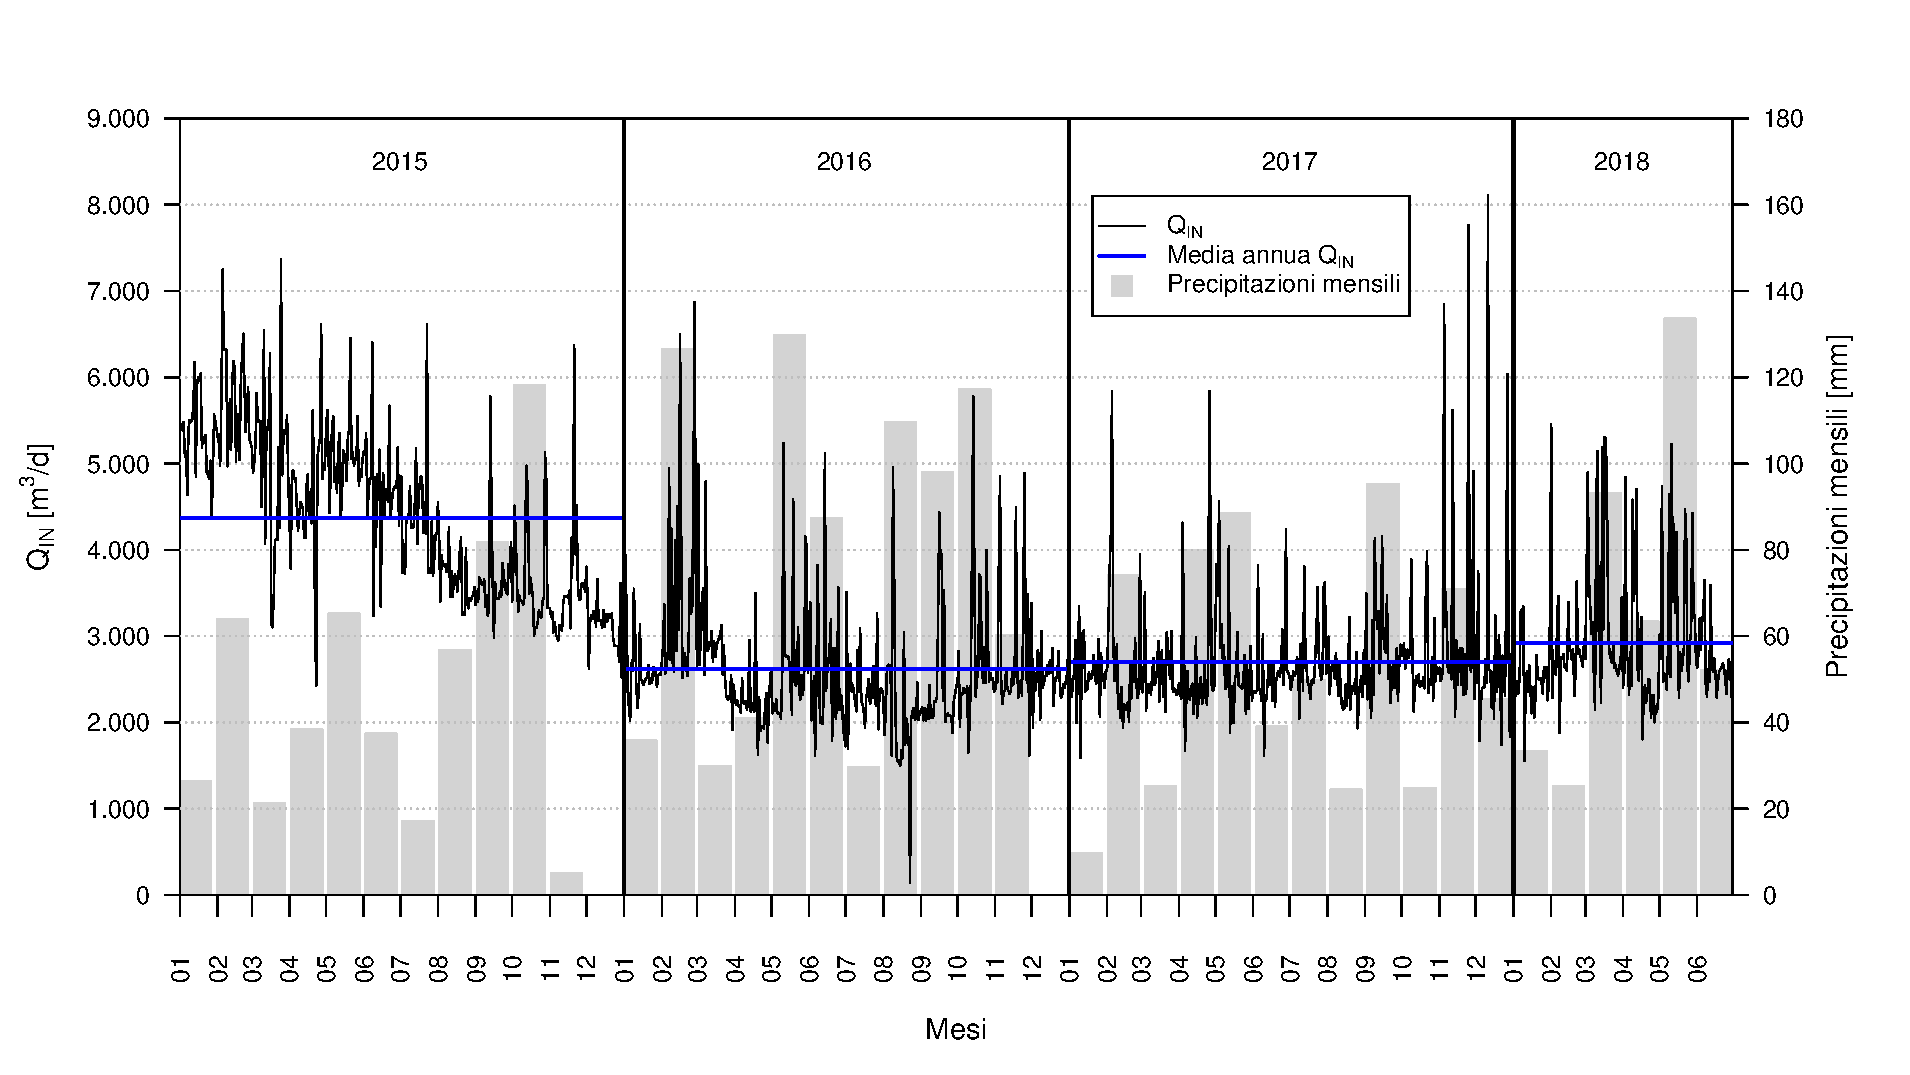
\includegraphics[width=\linewidth]{sa_qin-prec}}
	\centering
	\caption{Andamento della portata giornaliera in ingresso e  precipitazioni mensili}
	\label{fig:sa_qin-prec}
\end{figure}

\begin{table}[h]
\begin{center}
	\scriptsize
	\begin{tabular}{|>{\centering\arraybackslash}p{3,2cm}|>{\centering\arraybackslash}p{3,2cm}|>{\centering\arraybackslash}p{3,2cm}|>{\centering\arraybackslash}p{3,2cm}|}
		\hline 
		\textbf{Periodo} & \textbf{Media Q\textsubscript{IN} [m\textsuperscript{3}/d]} & \textbf{Mediana Q\textsubscript{IN} [m\textsuperscript{3}/d]} & \textbf{Media/Mediana [ - ]} \\ 
		\hline 
		2015 & 4.370 & 4.368 & 1,00 \\ 
		\hline 
		2016 & 2.620 & 2.461 & 1,06 \\ 
		\hline 
		2017 & 2.702 & 2.529 & 1,07 \\ 
		\hline 
		2018 & 2.921 & 2.661 & 1,09 \\ 
		\hline 
		2016 - 2018 & 2.713 & 2.532 & 1,07 \\ 
		\hline 
	\end{tabular} 
	\caption {Media, mediana e rapporto media/mediana delle portate in ingresso}
	\label{tab:sa_portate}
\end{center}
\end{table}
In \autoref{tab:sa_portate} sono riportati i valori della media, della mediana e del loro rapporto per ciascun anno e per il periodo complessivo compreso tra il 2016 e il 2018 (si è escluso il 2015 perché, visto l’andamento marcatamente decrescente, è poco rappresentativo).
Come valore di riferimento per la portata in tempo asciutto sarebbe opportuno considerare la mediana perché, a differenza della media, non è influenzata dai valori estremi presenti nella serie di dati. Si noti come, nel caso in esame, il rapporto tra media e mediana è prossimo all’unità.
Di conseguenza, per la portata in tempo asciutto per il periodo 2016 - 2018 può essere assunto il valore arrotondato di 2.500 m\textsuperscript{3}/d. Tale valore è di molto inferiore alla portata corrispondente alla potenzialità di progetto (30.000 AE), stimabile in circa 6.000 m\textsuperscript{3}/d.


\begin{figure}[h]
	\fbox{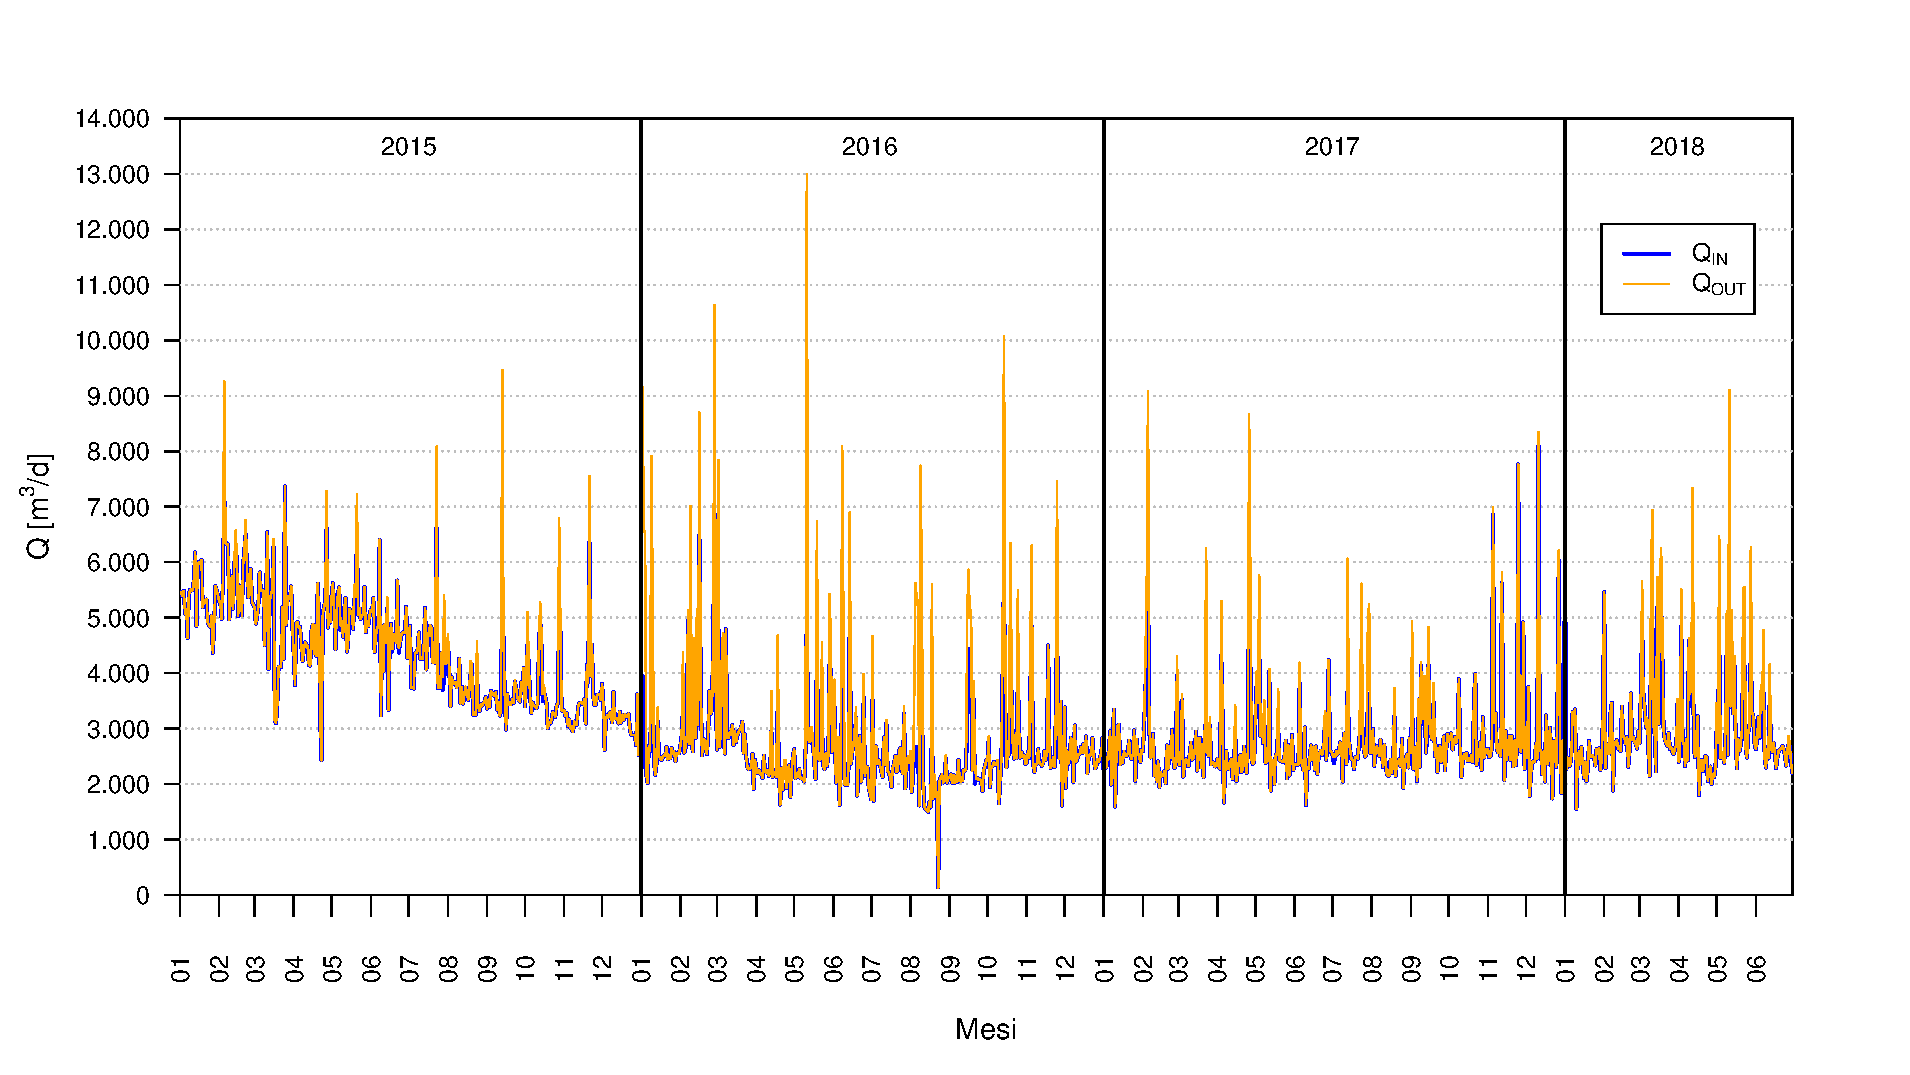
\includegraphics[width=\linewidth]{sa_qin-qout}}
	\centering
	\caption{Andamento delle portate giornaliere in ingresso e in uscita}
	\label{fig:sa_qin-qout}
\end{figure}

In \autoref{fig:sa_qin-qout}, invece, sono rappresentate la portata in ingresso all’impianto e la portata in uscita dallo stesso. In corrispondenza dei valori di punta si verifica by-pass della portata entrante al fine di non sovraccaricare idraulicamente l’impianto e di non compromettere l’efficienza dei trattamenti. Verosimilmente tali situazioni si hanno in caso di precipitazioni meteoriche significative.
La portata in uscita è data dalla somma della portata in ingresso all’impianto e della portata che non subisce trattamenti.
\pagebreak	
\paragraph{Caratteristiche qualitative}

\begin{figure}[h]
	\fbox{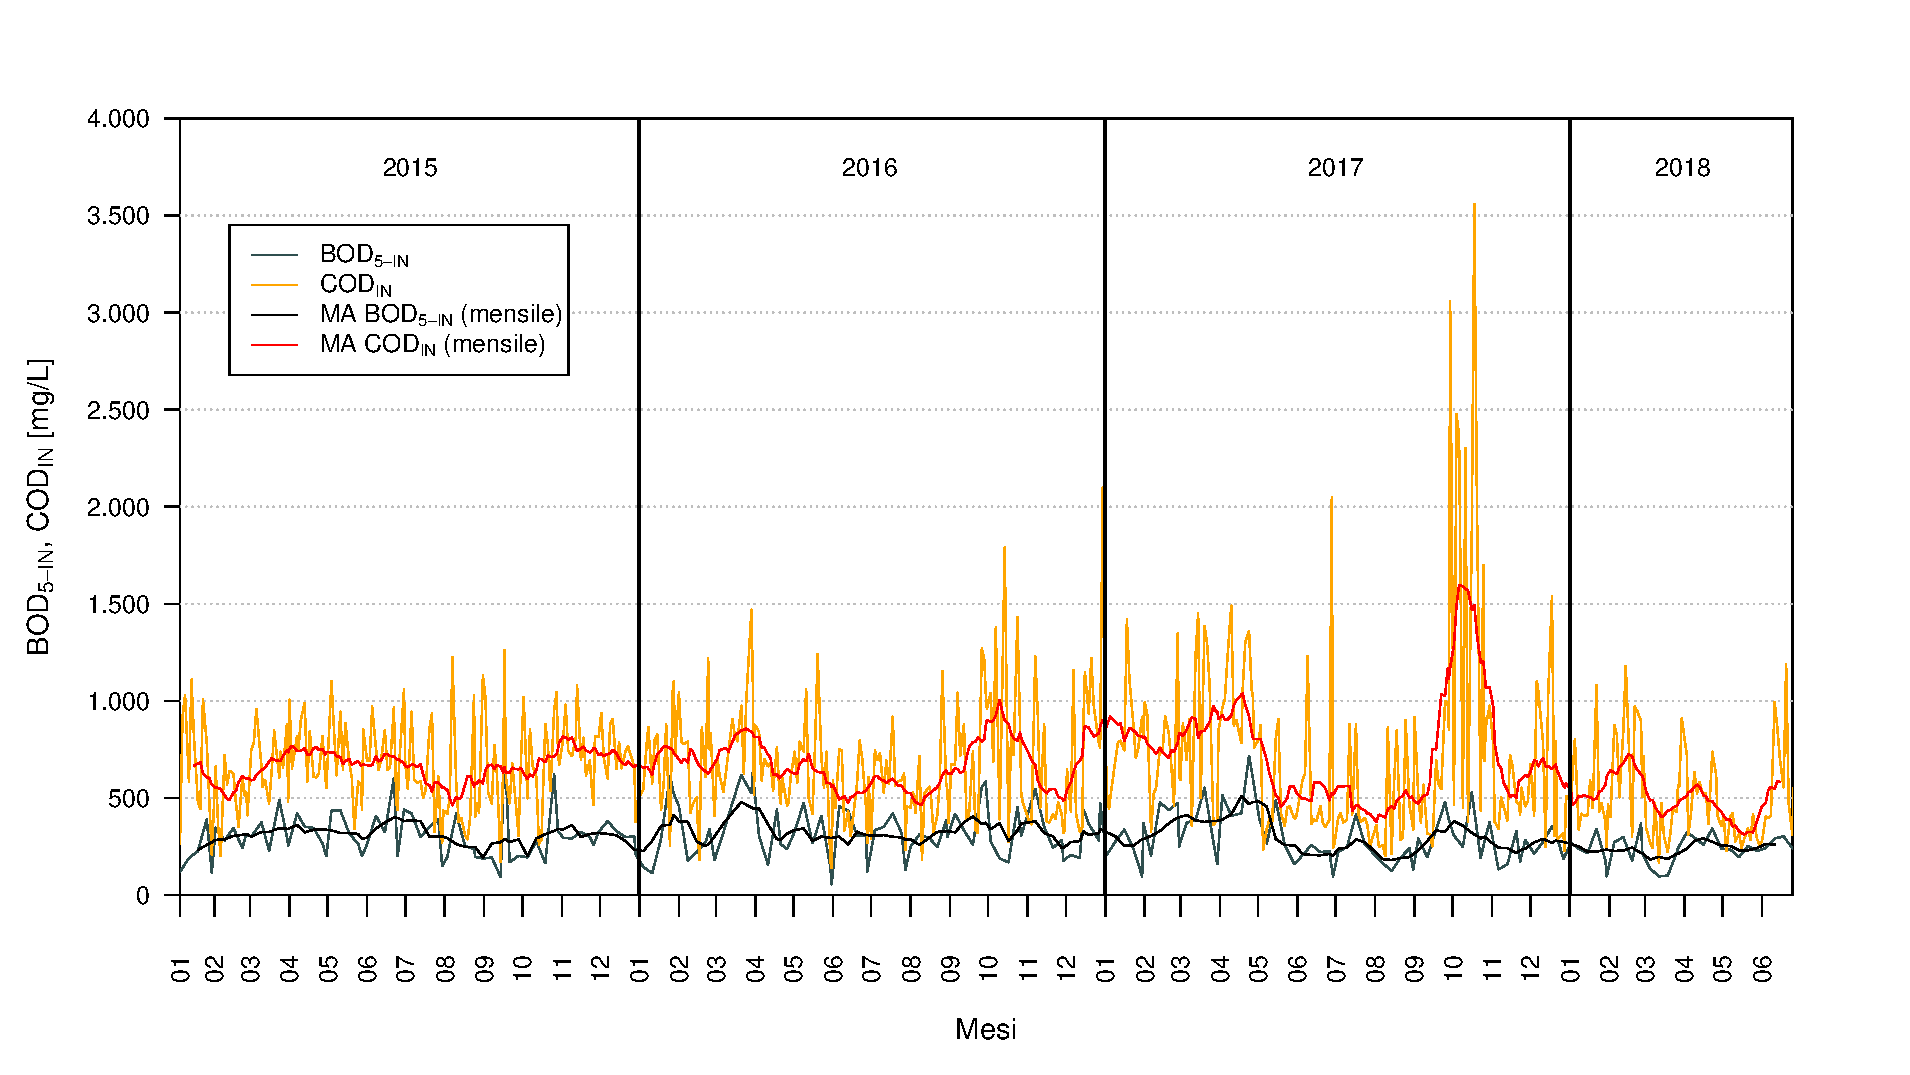
\includegraphics[width=\linewidth]{sa_BOD-COD}}
	\centering
	\caption{Andamento delle concentrazioni in ingresso di BOD\textsubscript{5} e COD}
	\label{fig:sa_BOD-COD}
\end{figure}

L’andamento delle concentrazioni di BOD\textsubscript{5} e COD, ottenute attraverso il campionamento routinario, è mostrato in \autoref{fig:sa_BOD-COD}.
Entrambe le concentrazioni presentano una discreta variabilità. Il COD si mantiene nell'intervallo 500-1.000 mg/L (come media mobile), il BOD\textsubscript{5} nell'intervallo 150-500 mg/L. Questi valori sono tipici di un liquame a concentrazione media-forte (\autoref{tab:conc_tipiche}). In particolare, per quanto riguarda il COD, si nota una tendenza all’incremento tra settembre e novembre degli anni 2016 e 2017 e tra dicembre 2016 e maggio 2017. In questi periodi si raggiungono occasionalmente anche picchi oltre i 2.000 mg/L. Queste variazioni potrebbero essere causate da attività vitivinicole allacciate alla pubblica fognatura (è in corso un censimento da parte del gestore).
BOD\textsubscript{5} e COD, come ci si aspetta, sono correlati (osservare la media mobile aiuta nell’individuazione di tale correlazione) anche se, in corrispondenza di importanti aumenti di COD, si verificano incrementi di BOD\textsubscript{5} meno accentuati.

\begin{figure}[H]
	\fbox{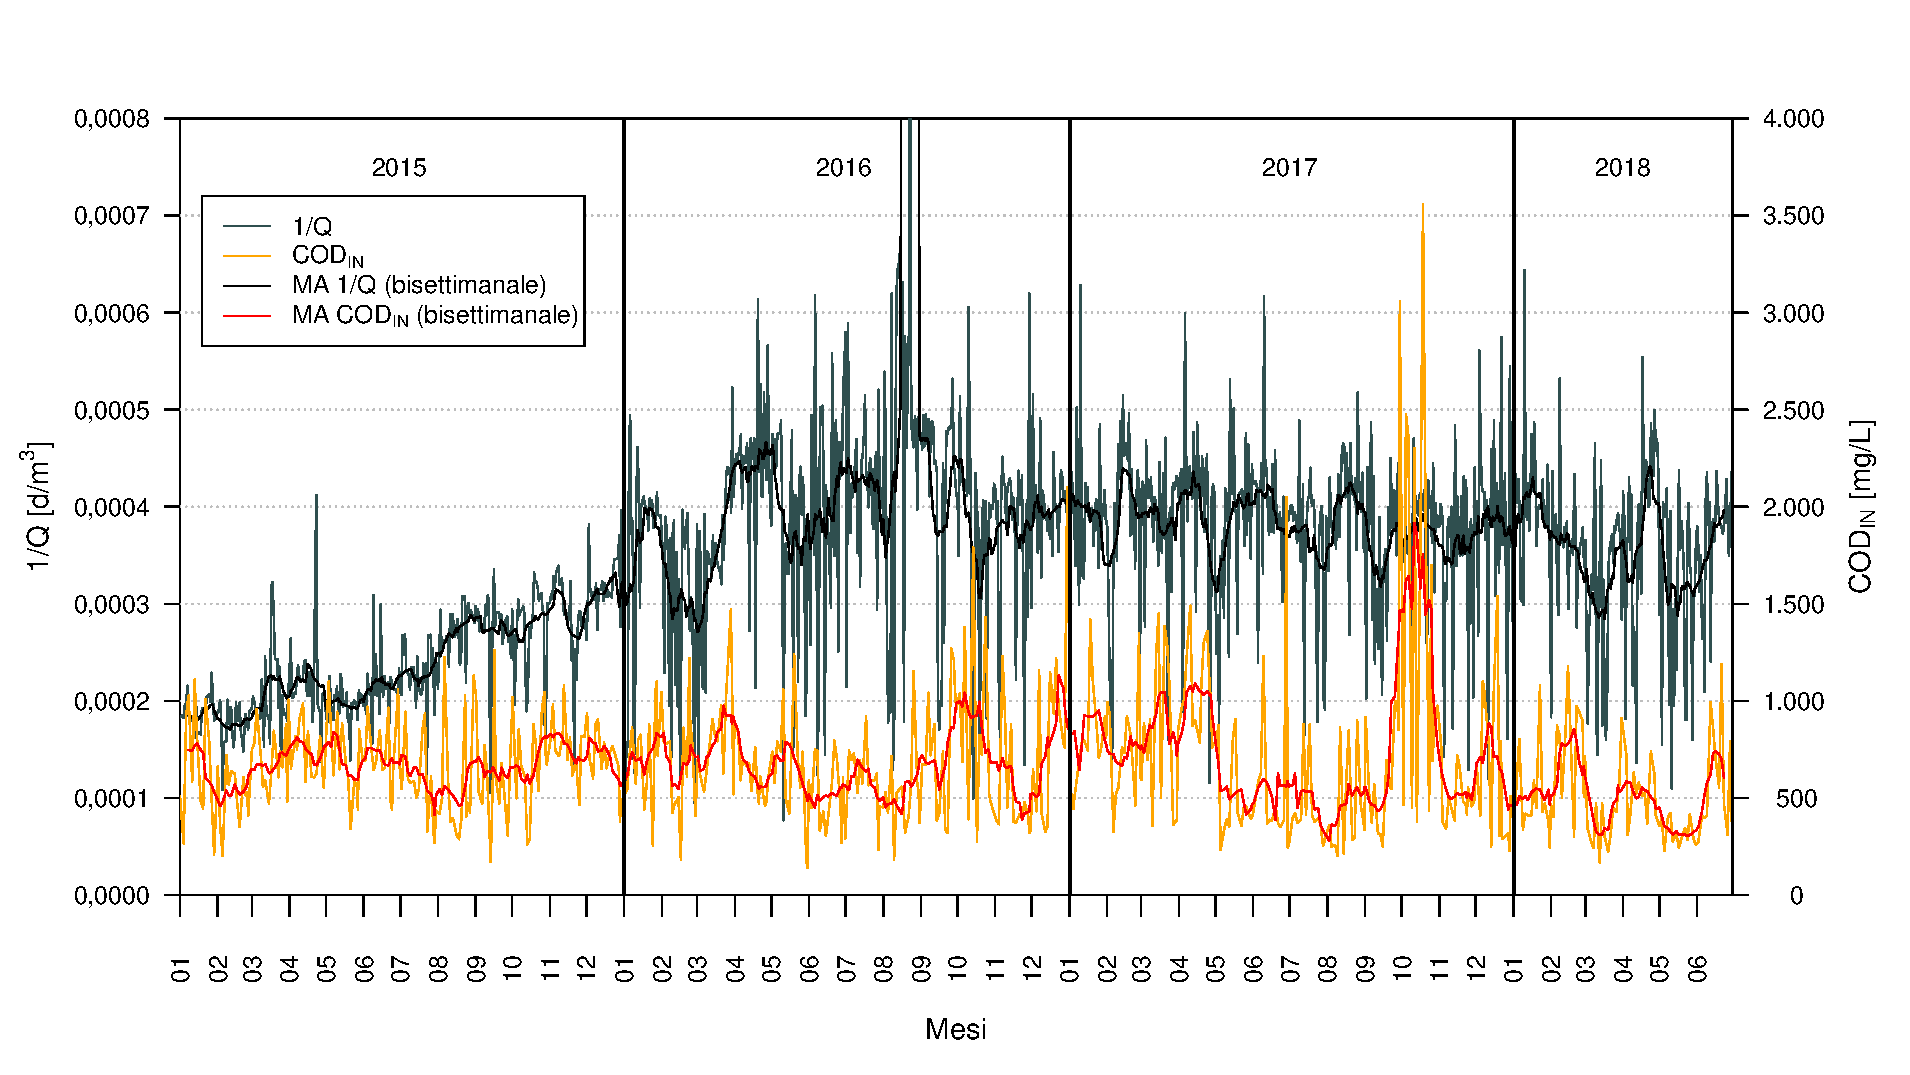
\includegraphics[width=\linewidth]{sa_COD-1q}}
	\centering
	\caption{Andamento della concentrazione in ingresso di COD e dell'inverso della portata giornaliera}
	\label{fig:sa_COD-1q}
\end{figure}
\begin{figure}[H]
	\fbox{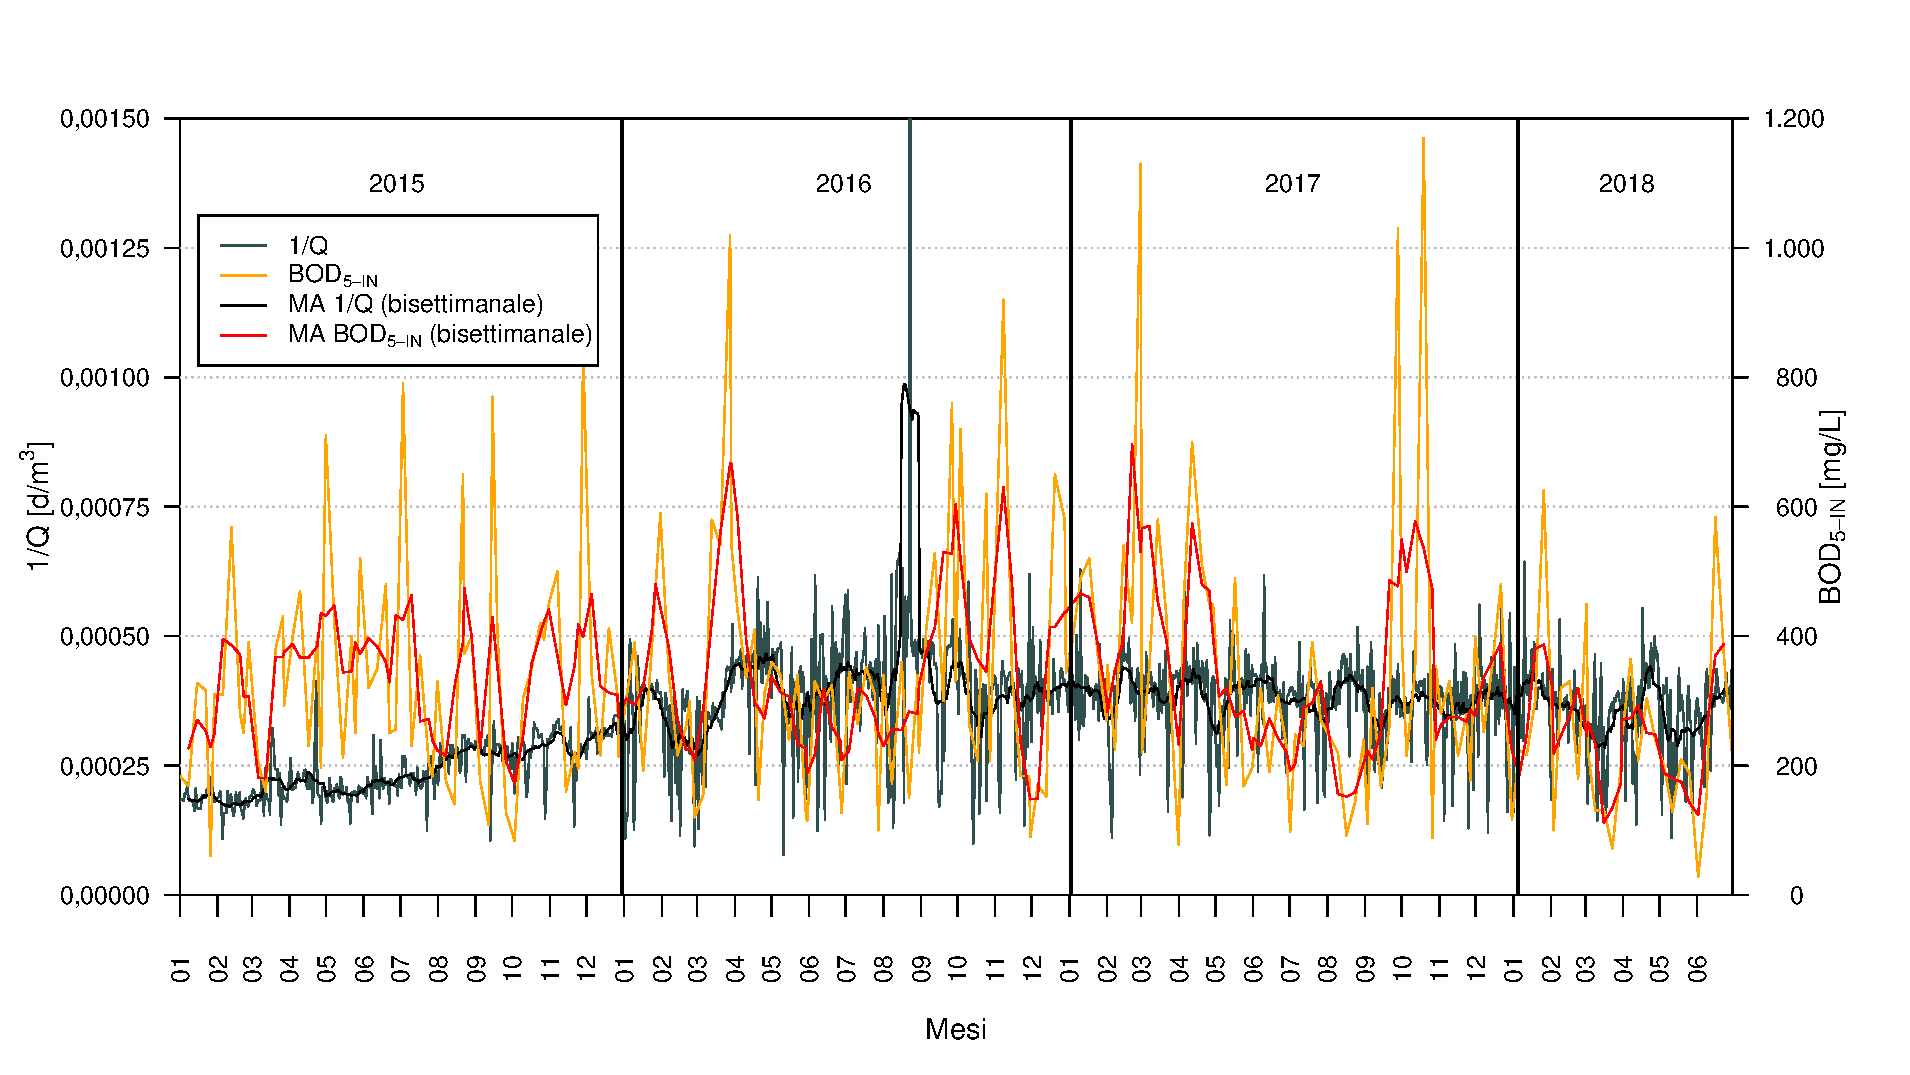
\includegraphics[width=\linewidth]{sa_BOD-1q}}
	\centering
	\caption{Andamento della concentrazione in ingresso di BOD\textsubscript{5} e dell'inverso della portata giornaliera}
	\label{fig:sa_BOD-1q}
\end{figure}

I grafici di \autoref{fig:sa_COD-1q} e \autoref{fig:sa_BOD-1q} riportano i valori di concentrazione di COD e BOD\textsubscript{5} e l’inverso della portata giornaliera al fine di verificare se le variazioni di concentrazione siano correlate alla portata.
Con riferimento all’anno 2015, la diminuzione di portata non ha effetti sulla concentrazione di COD che non presenta alcun tipo di trend. Anche nei periodi del 2016 e del 2017 caratterizzati da elevati valori di COD, non si individua correlazione stabile, ma solo per periodi limitati. In altre fasi temporali, anche quando la portata è piuttosto stabile, il COD presenta valori molto elevati, per cui si può affermare di avere un refluo più ricco di carico organico.
Non avendo riconosciuto correlazione, si può concludere che l’andamento della concentrazione di COD non è influenzato dalla variazione della portata, ma sarà da imputare a cause esterne come, per esempio, scarichi di tipo non domestico.
Osservazioni analoghe possono essere fatte relativamente al BOD\textsubscript{5}.

\begin{figure}[H]
	\fbox{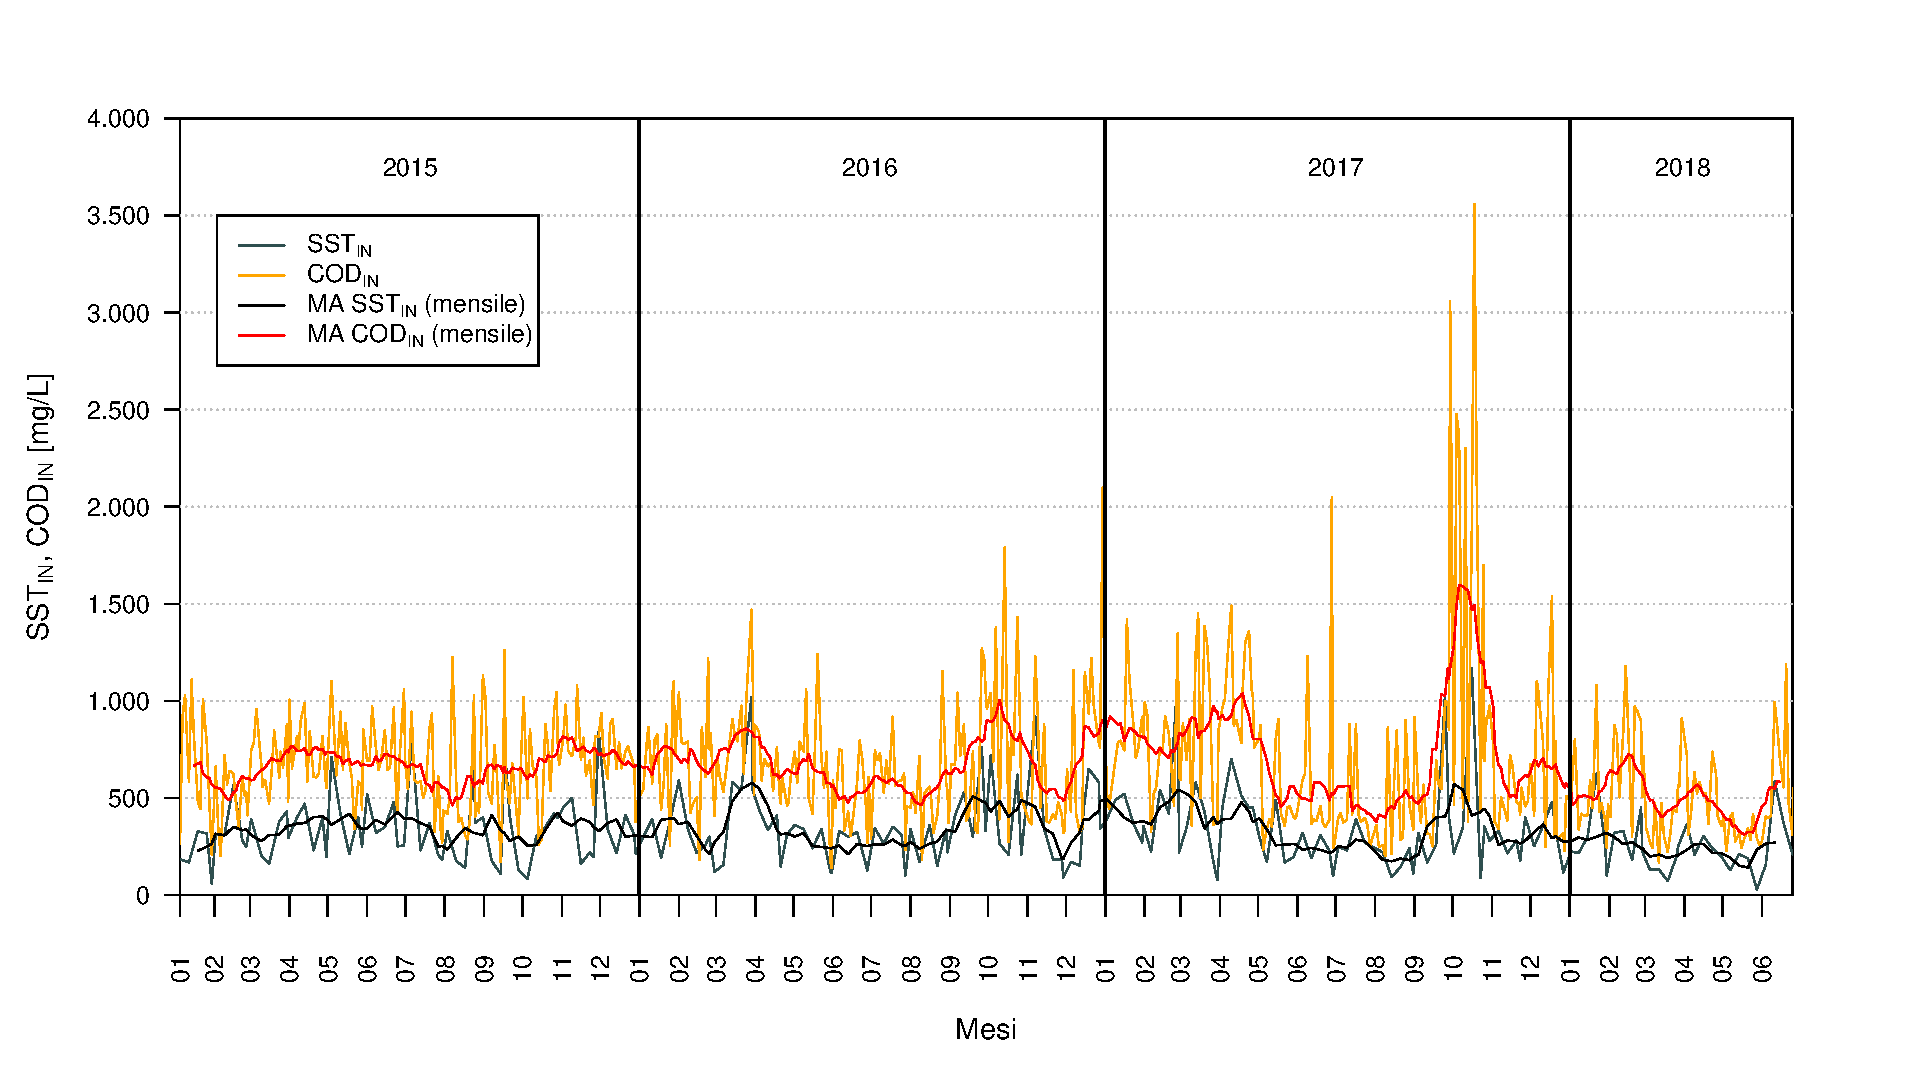
\includegraphics[width=\linewidth]{sa_COD-SST}}
	\centering
	\caption{Andamento delle concentrazioni in ingresso di COD e di SST}
	\label{fig:sa_COD-SST}
\end{figure}
\begin{figure}[H]
	\fbox{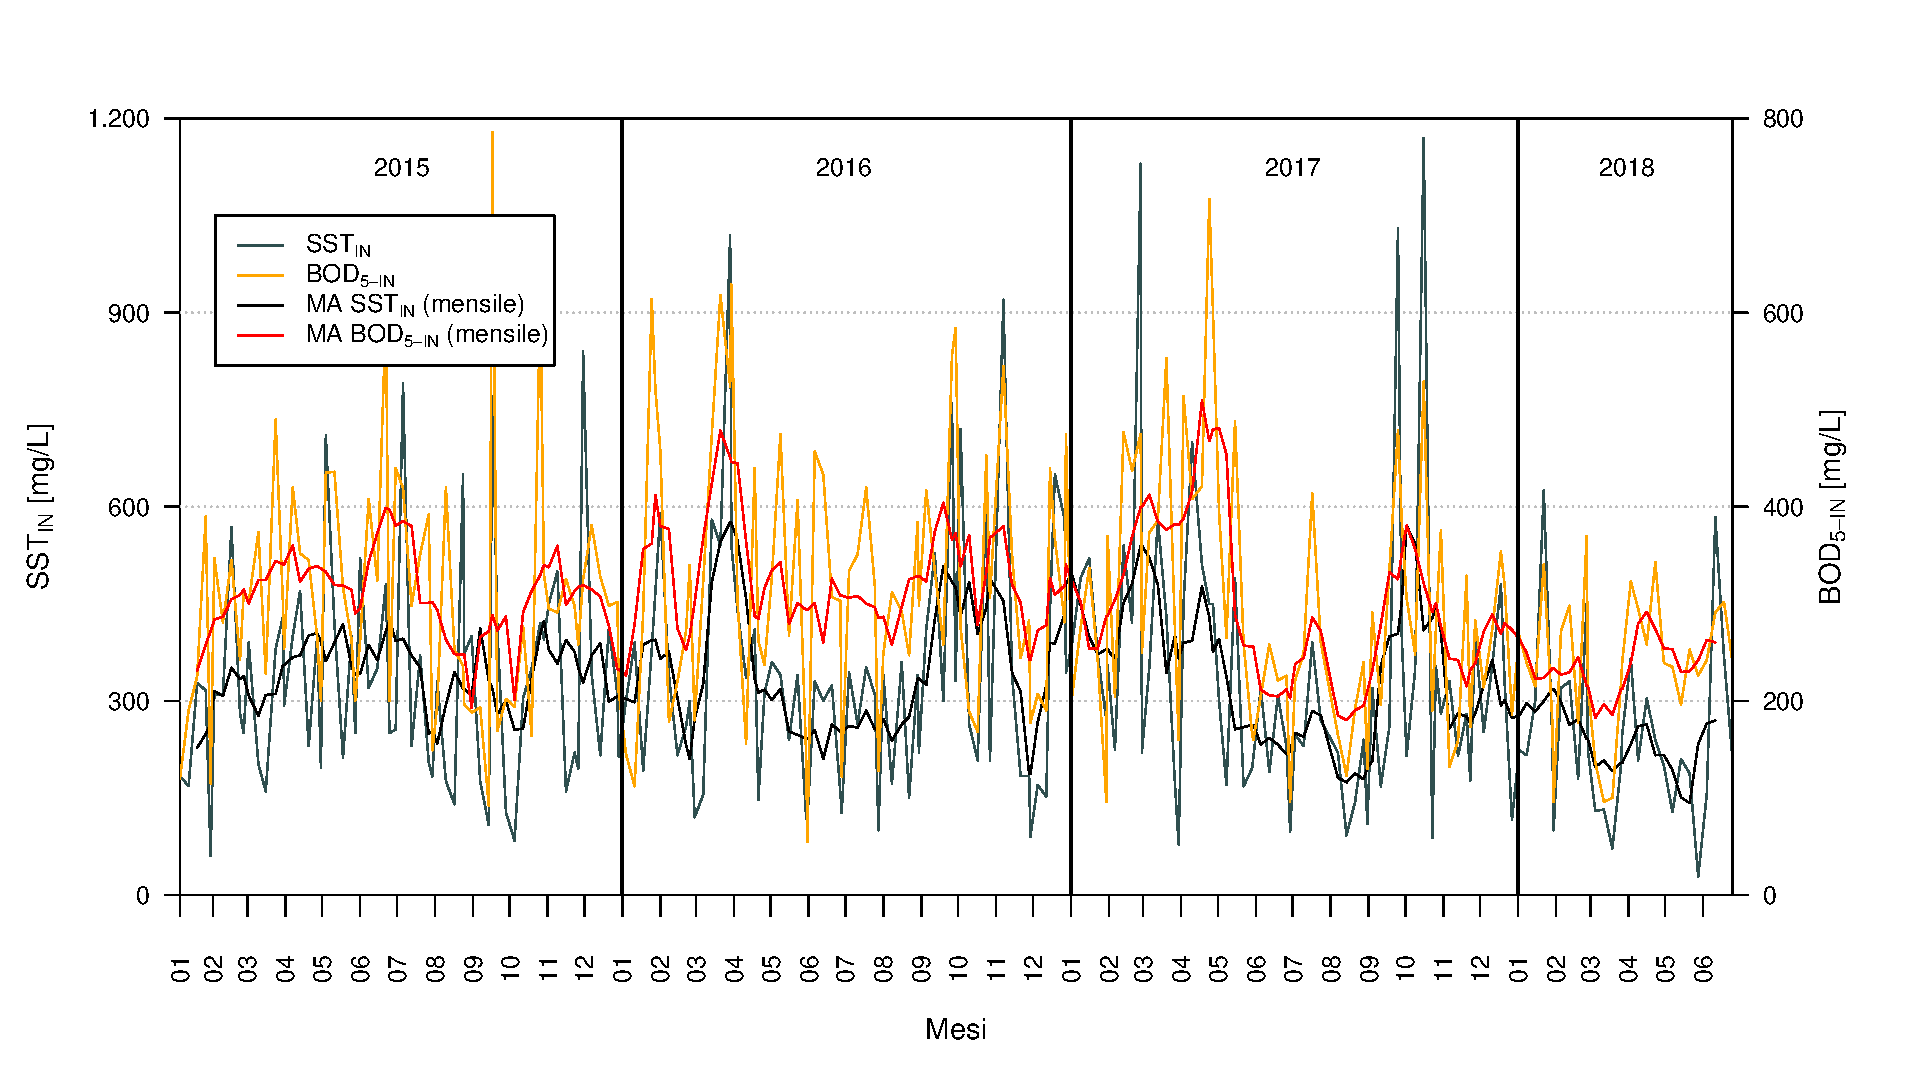
\includegraphics[width=\linewidth]{sa_BOD-SST}}
	\centering
	\caption{Andamento delle concentrazioni in ingresso di BOD\textsubscript{5} e di SST}
	\label{fig:sa_BOD-SST}
\end{figure}

Nella \autoref{fig:sa_COD-SST} è mostrato l’andamento della concentrazione di COD e di SST e si vede chiaramente che c’è correlazione tra le due grandezze.

Nella \autoref{fig:sa_BOD-SST}, invece, si ha il confronto tra BOD\textsubscript{5} e SST che individua ancora una buona correlazione.

\begin{figure}[H]
	\fbox{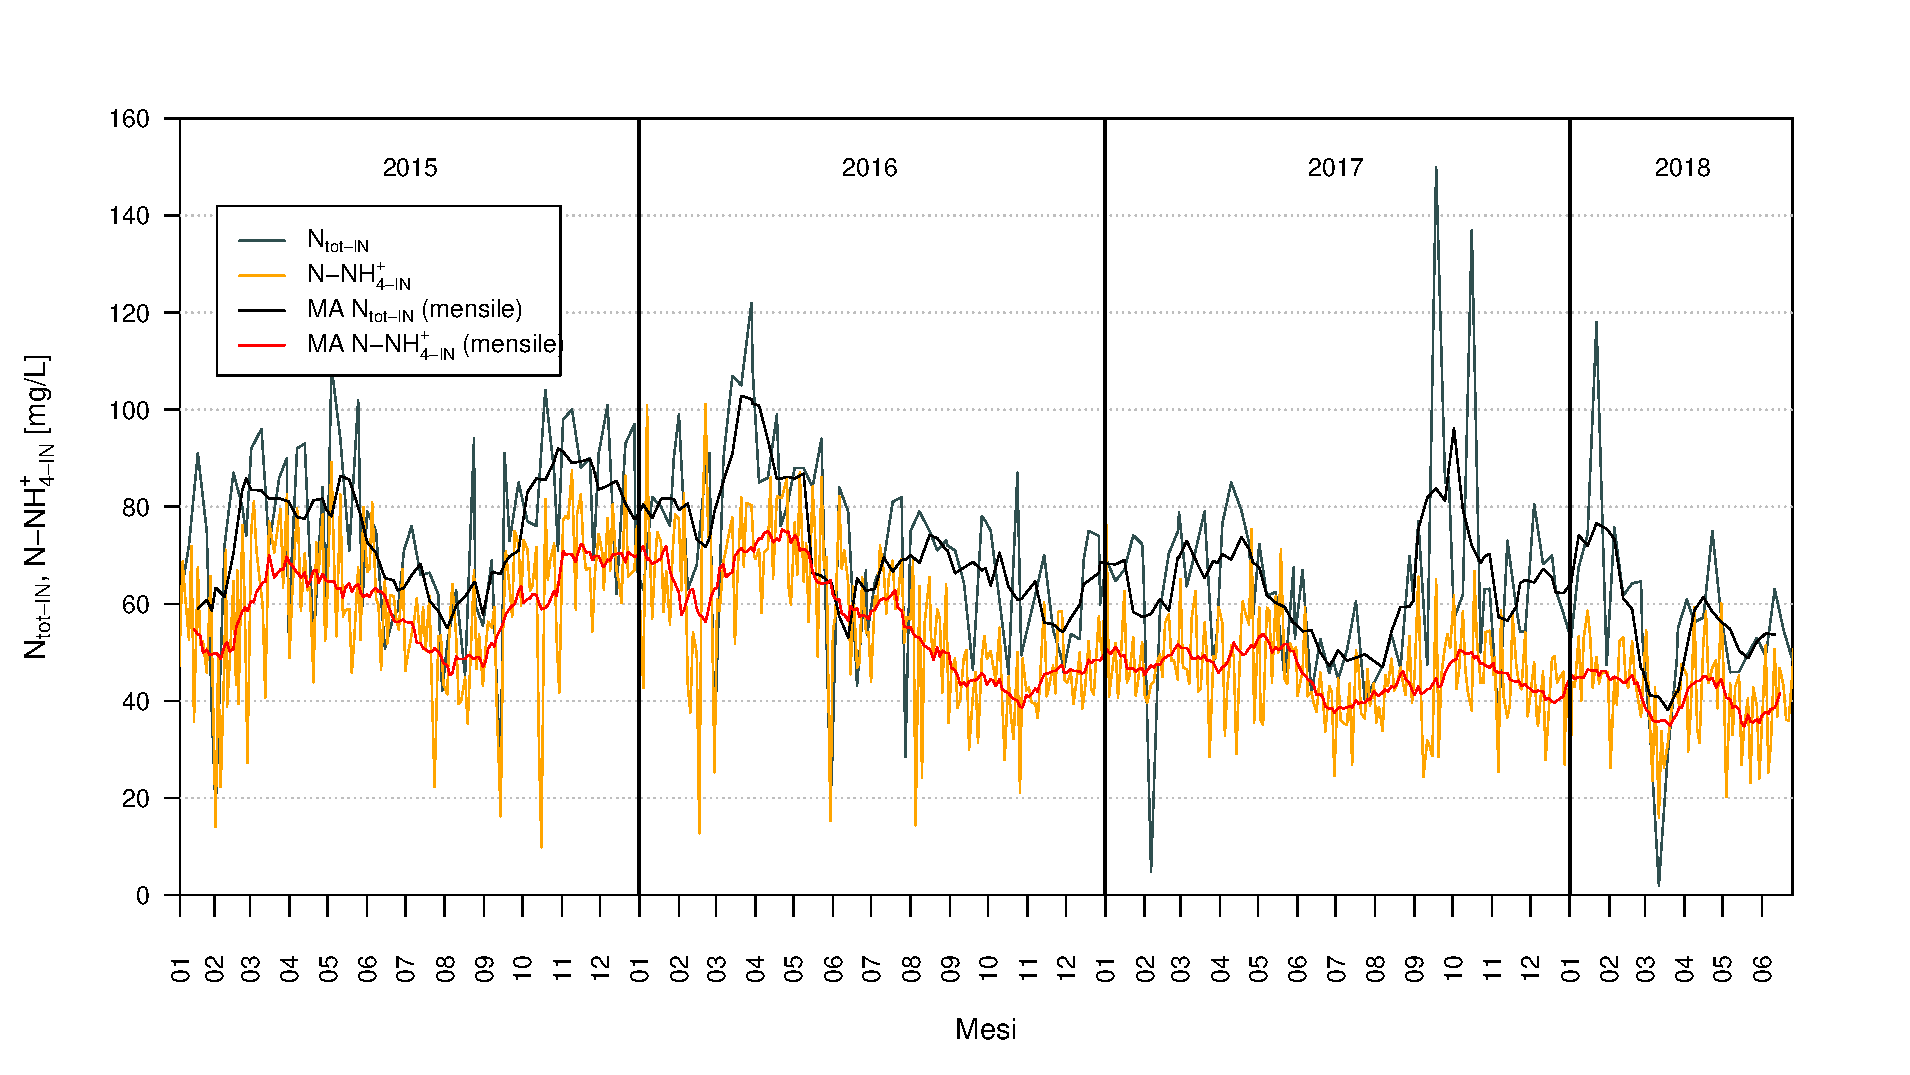
\includegraphics[width=\linewidth]{sa_Ntot-NNH4+}}
	\centering
	\caption{Andamento delle concentrazioni in ingresso di azoto totale e azoto ammoniacale}
	\label{fig:sa_Ntot-NNH4+}
\end{figure}

L’andamento dell’azoto totale e dell’azoto ammoniacale è riportato in \autoref{fig:sa_Ntot-NNH4+}.
Entrambe le grandezze sono notevolmente variabili e in molti casi superano gli 85 mg/L per l’azoto totale e 50 mg/L per quello ammoniacale, tipici di un liquame domestico fortemente concentrato (\autoref{tab:conc_tipiche}). Ciò potrebbe dipendere, come già visto anche per il COD, dalla presenza di scarichi di diverso tipo rispetto a quelli urbani come scarichi di allevamenti o scarichi provenienti da attività vitivinicole.
Se si escludono i picchi di fine 2017 e inizio 2018, è possibile riconoscere un trend leggermente decrescente che ha inizio nella prima metà dell’anno 2016. 
In termini di percentuale, l’azoto ammoniacale è la maggior componente dell’azoto totale, come previsto per un refluo di origine civile (mediamente rappresenta l'80\%).

\begin{figure}[H]
	\fbox{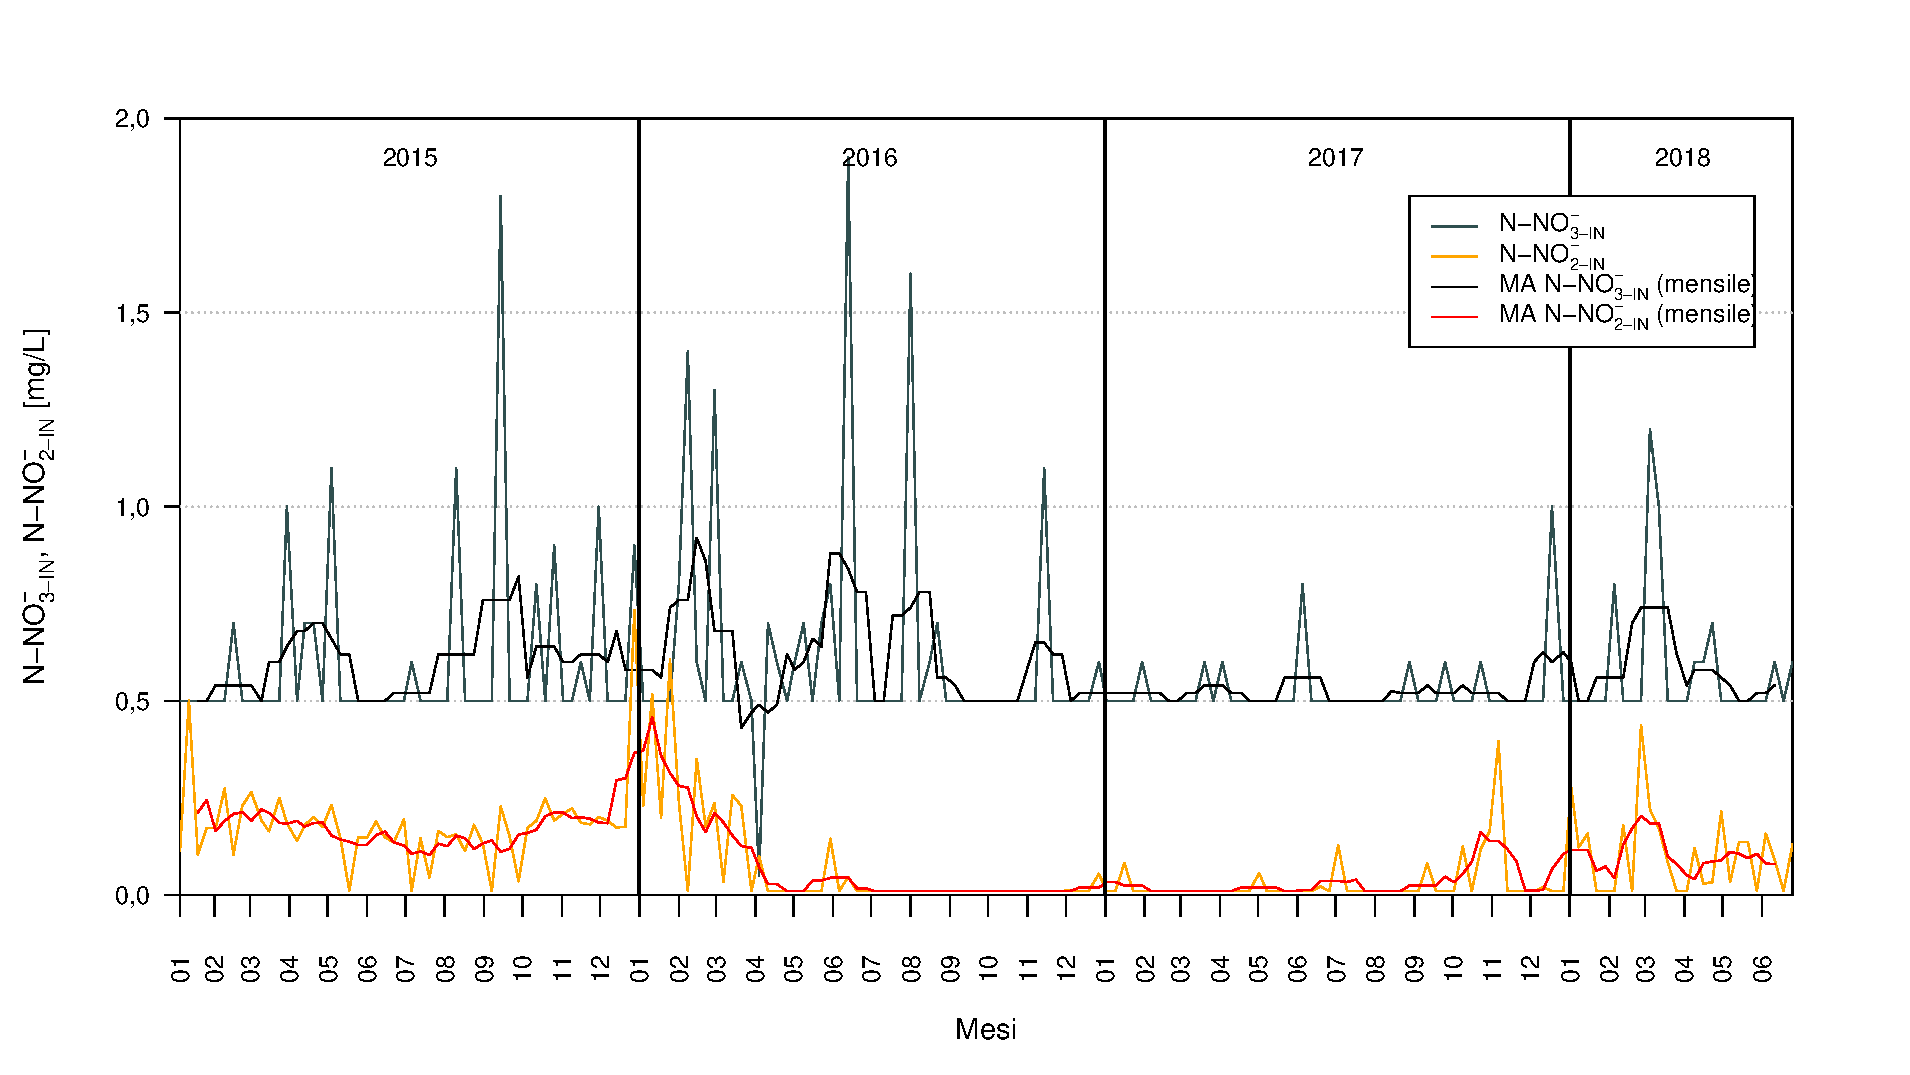
\includegraphics[width=\linewidth]{sa_NO2-NO3}}
	\centering
	\caption{Andamento delle concentrazioni in ingresso di azoto nitroso e azoto nitrico}
	\label{fig:sa_NO2-NO3}
\end{figure}

La percentuale di azoto nitroso e nitrico, invece, è irrisoria (\autoref{fig:sa_NO2-NO3}): le forme azotate ossidate non superano mai i 2 mg/L, mentre il valore medio della concentrazione di azoto totale è di circa 70 mg/L.

Analogamente a quanto fatto precedentemente per il COD, si sono messe a confronto le concentrazioni di azoto totale  con l’inverso della portata giornaliera (\autoref{fig:sa_Ntot-1q}).
Anche in questo caso non si manifesta alcuna correlazione e quindi non è possibile trovare corrispondenza tra la variazione di portata e di concentrazione di azoto totale.
\begin{figure}[H]
	\fbox{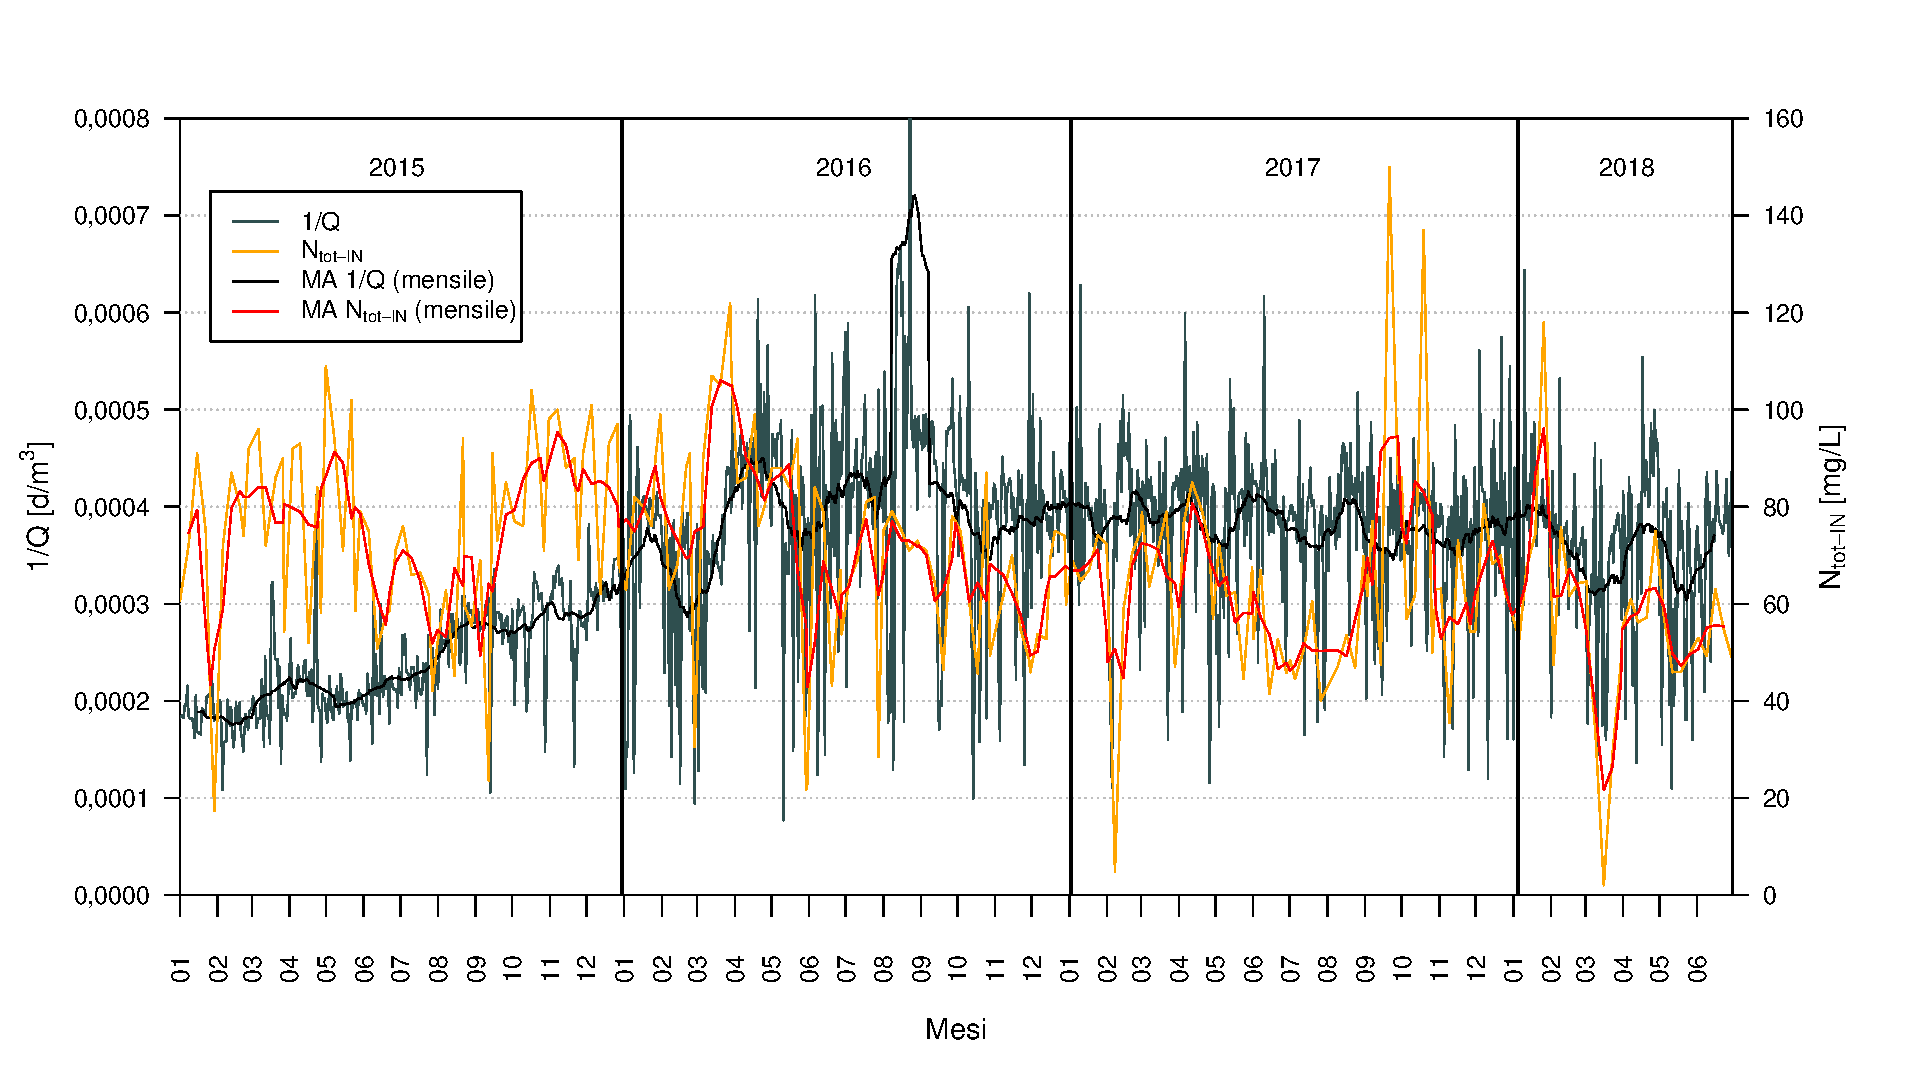
\includegraphics[width=\linewidth]{sa_Ntot-1q}}
	\centering
	\caption{Andamento della concentrazione in ingresso di azoto totale e dell'inverso della portata giornaliera}
	\label{fig:sa_Ntot-1q}
\end{figure}
\begin{figure}[H]
	\fbox{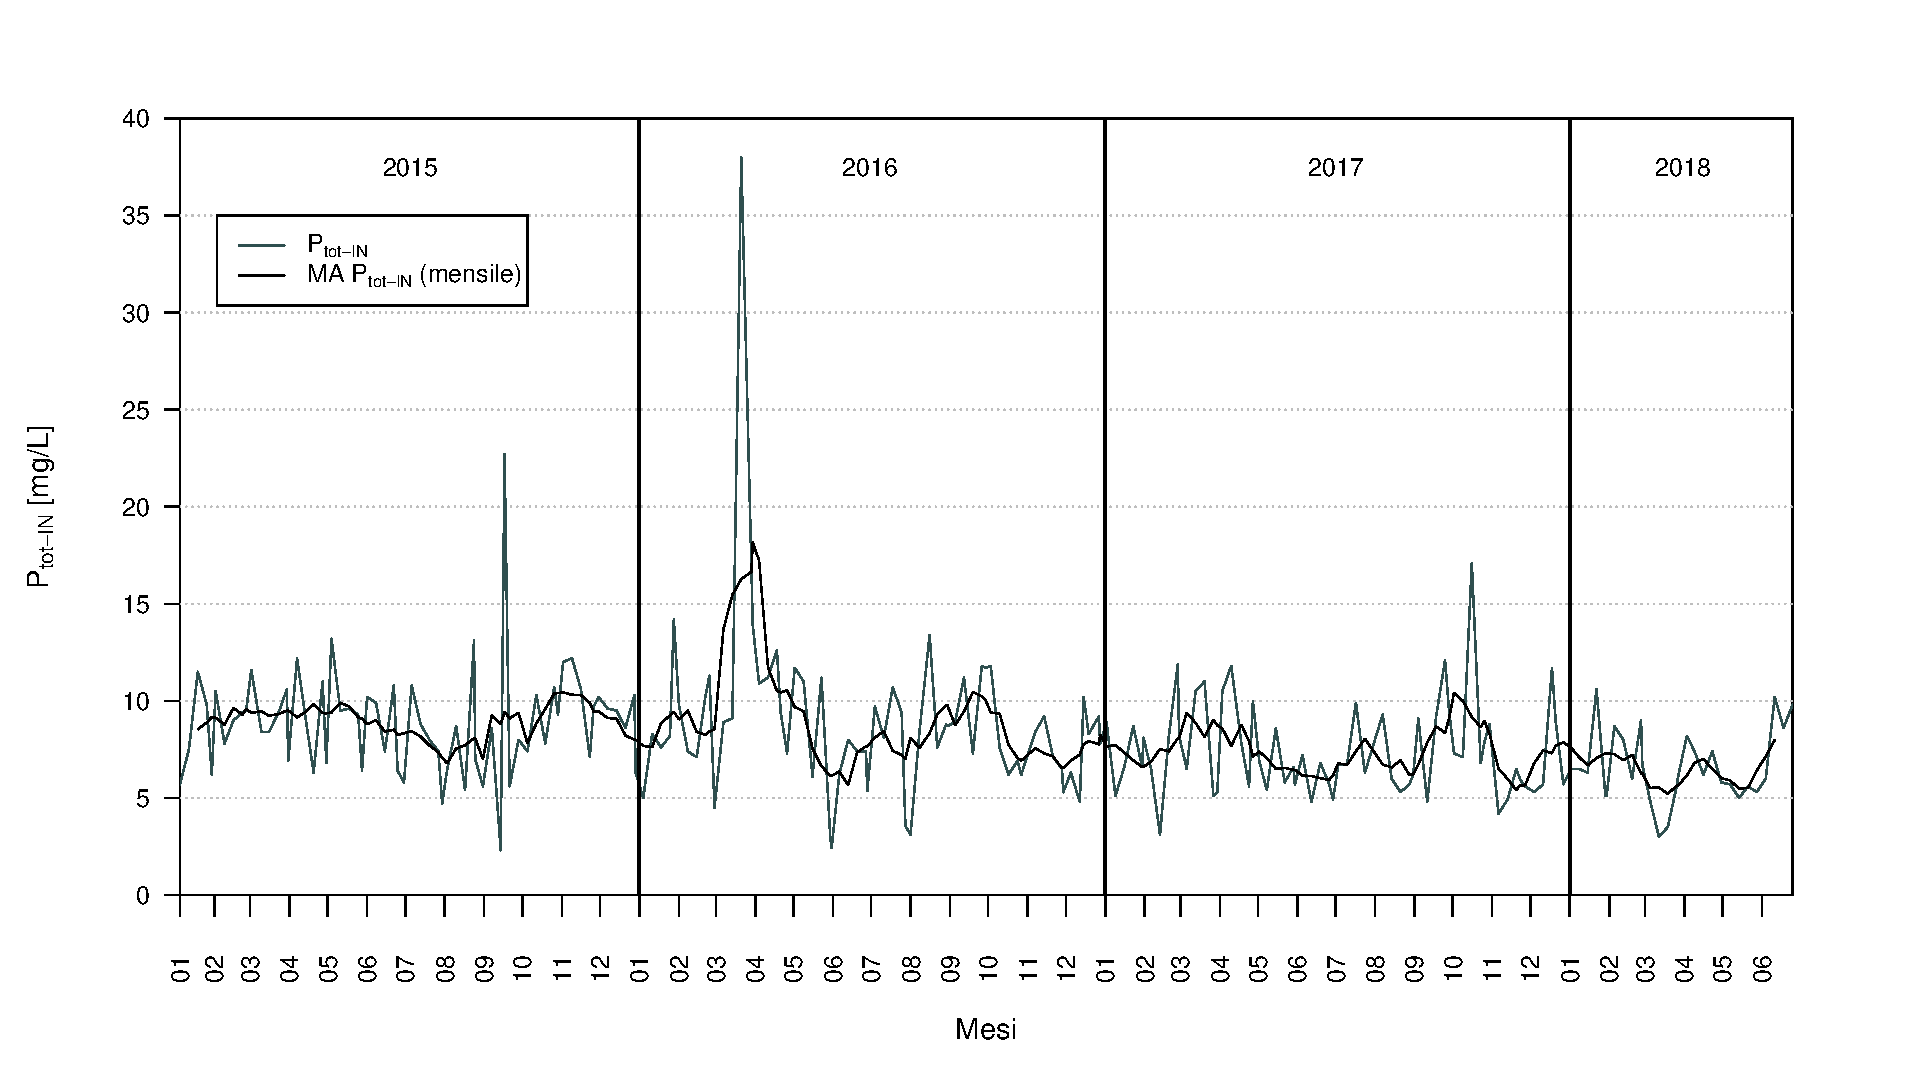
\includegraphics[width=\linewidth]{sa_Ptot}}
	\centering
	\caption{Andamento della concentrazione in ingresso di fosforo totale}
	\label{fig:sa_Ptot}
\end{figure}

In \autoref{fig:sa_Ptot} sono mostrate le oscillazioni della concentrazione di fosforo totale in ingresso all’impianto.
Poiché i dati in esame frequentemente si avvicinano o superano i 10 mg/L (liquame fortemente concentrato), sempre a conferma di quanto già stabilito, è probabile che il liquame in arrivo all’impianto comprenda anche reflui di provenienza diversa da quella civile. Come per l'azoto, si osserva un trend leggermente decrescente.\\

Di seguito sono stati analizzati i valori dei rapporti tra le concentrazioni dei diversi inquinanti e sono stati confrontati con i valori di riferimento per un liquame urbano presentati in \autoref{tab:ppc_rapporti}.

\begin{figure}[H]
	\fbox{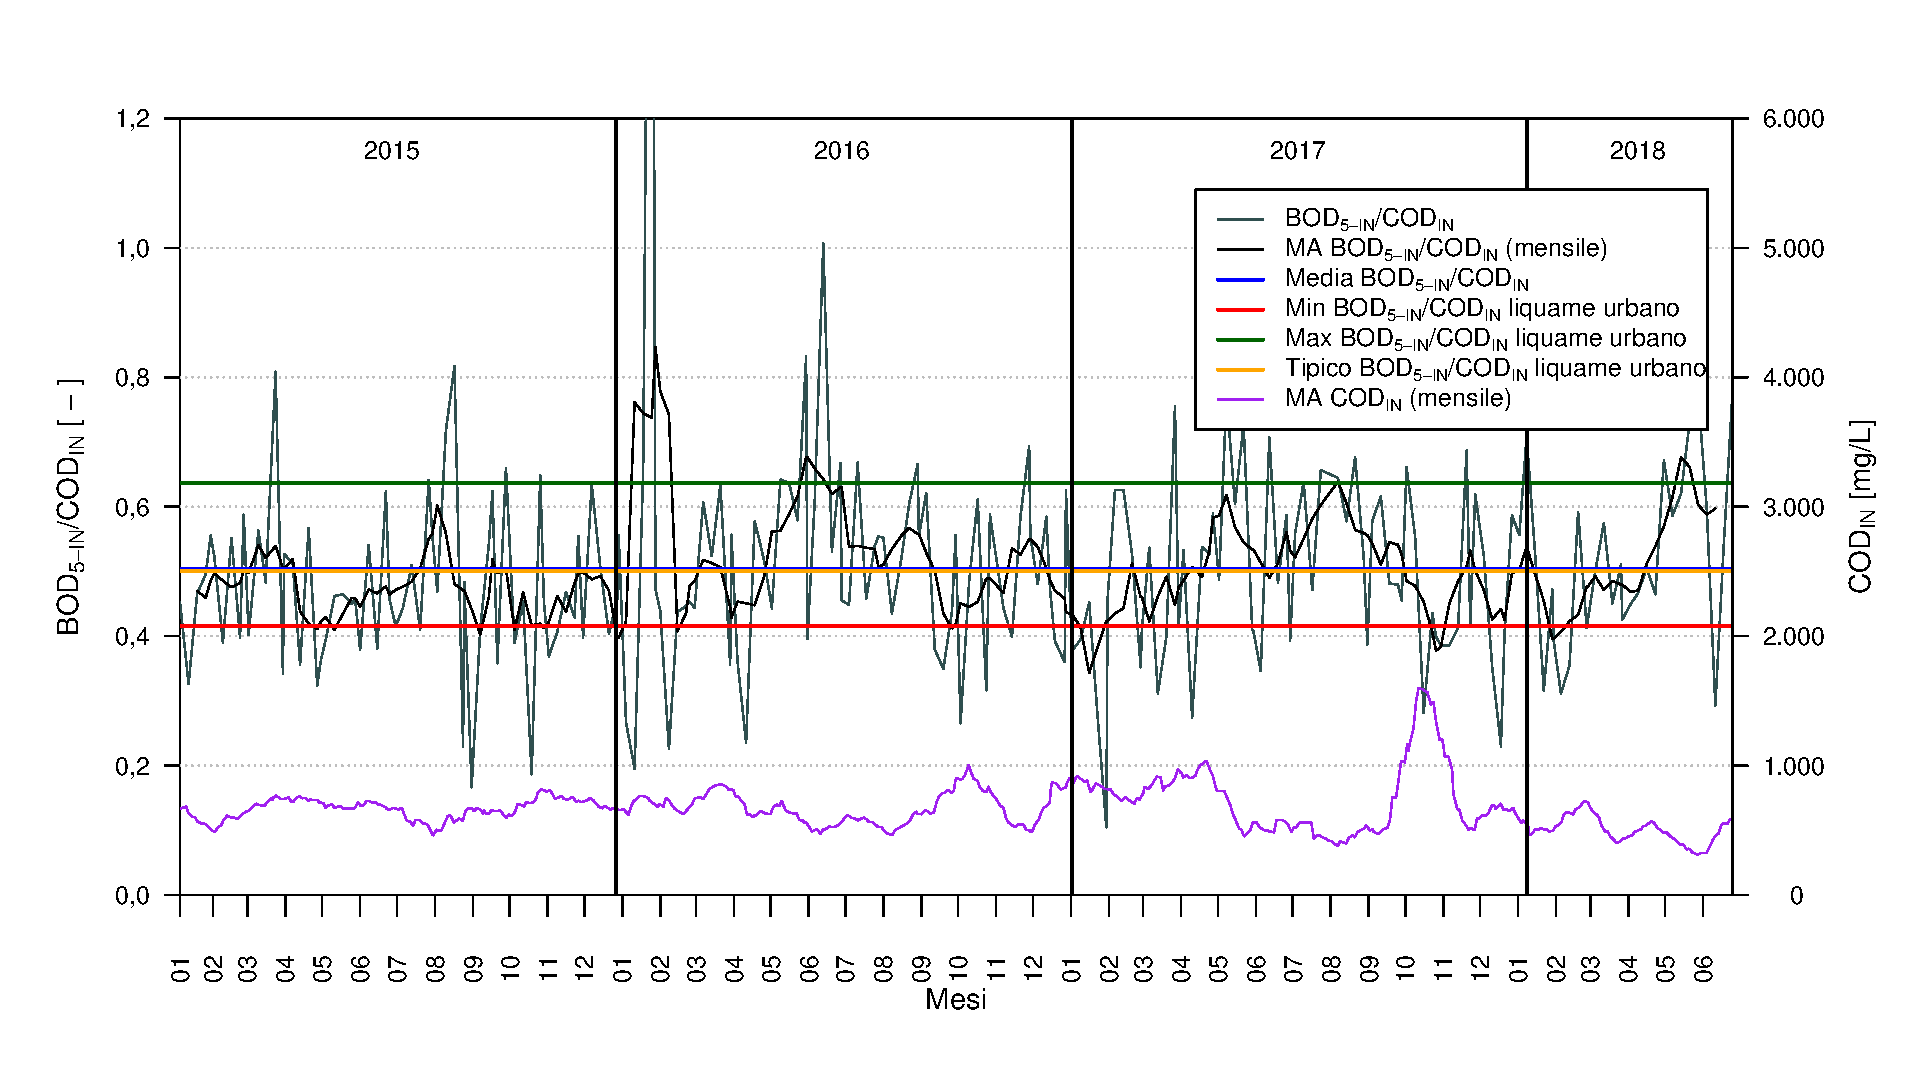
\includegraphics[width=\linewidth]{sa_BOD_COD}}
	\centering
	\caption{Andamento del rapporto tra BOD\textsubscript{5} e COD in ingresso}
	\label{fig:sa_BOD_COD}
\end{figure}

Il rapporto tra BOD\textsubscript{5} e COD è molto variabile anche se, confrontandolo con i valori di riferimento per un liquame urbano, si osserva che la media coincide con il valore tipico (0,5) e le oscillazione sono, per la maggior parte, comprese tra il massimo e il minimo (\autoref{fig:sa_BOD_COD}).
L’andamento della media mobile permette di vedere con facilità che nei mesi estivi il rapporto aumenta e si individua quindi una periodicità. 
Se si osserva anche l’andamento del COD, si nota che, quando quest’ultimo cresce molto, il rapporto si abbassa. Ciò è una conferma di quanto affermato analizzando il grafico di \autoref{fig:sa_BOD-COD}, ovvero che, quando il COD cresce in maniera significativa, il BOD\textsubscript{5} non segue tale andamento.

\begin{figure}[H]
	\fbox{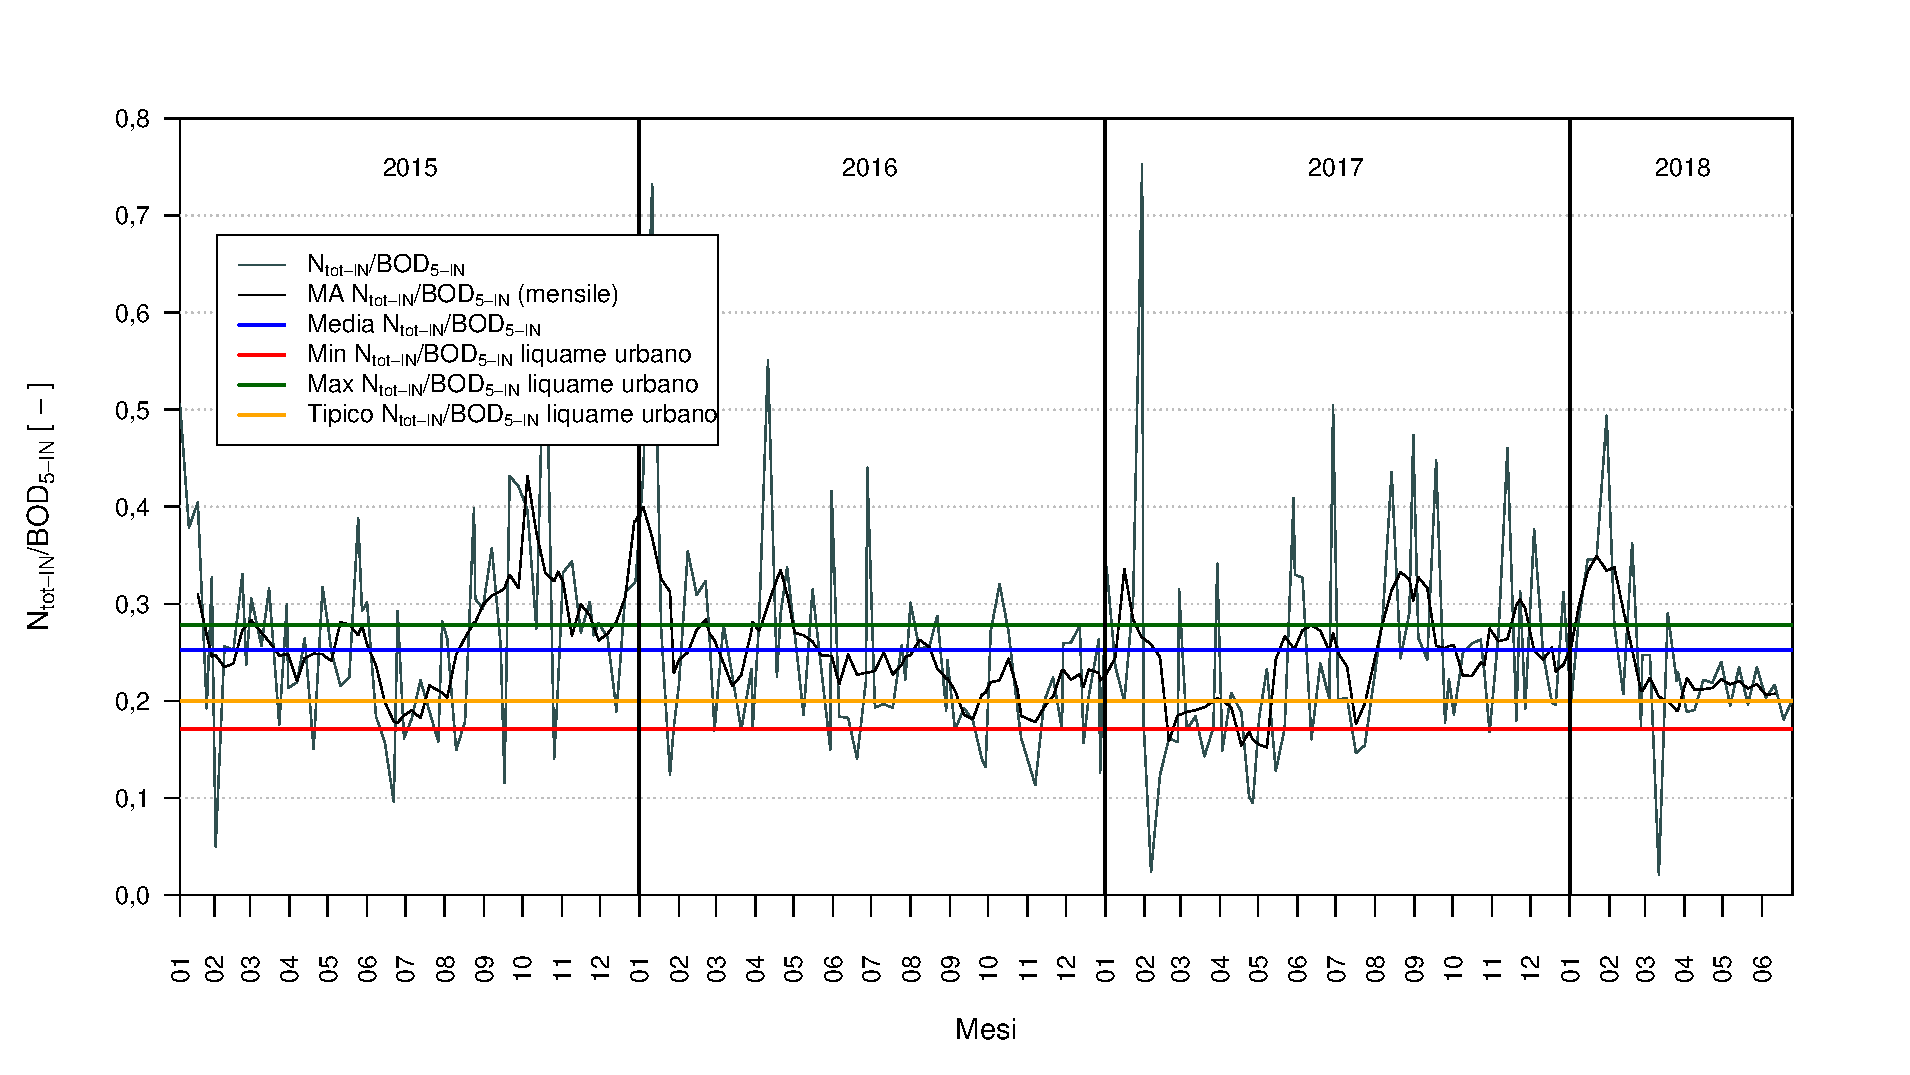
\includegraphics[width=\linewidth]{sa_Ntot_BOD}}
	\centering
	\caption{Andamento del rapporto tra azoto totale e BOD\textsubscript{5} in ingresso}
	\label{fig:sa_Ntot_BOD}
\end{figure}

Si ragioni ora sull’andamento dei rapporti tra azoto totale e BOD\textsubscript{5} e azoto totale e COD.
Il rapporto N\textsubscript{tot}/BOD\textsubscript{5} (\autoref{fig:sa_Ntot_BOD}) è molto variabile e quindi non c’è correlazione tra le due grandezze. 
Con riferimento anche alla \autoref{fig:sa_Ntot-NNH4+} (N\textsubscript{tot}) e alla \autoref{fig:sa_BOD-COD} (BOD\textsubscript{5}), si riscontra che, essendo il BOD\textsubscript{5} variabile ma privo di particolari tendenze, i tratti crescenti degli anni 2015 e 2017 e il tratto decrescente del 2016 dipendono dalle variazioni di concentrazione dell’azoto totale.
La media del rapporto si discosta dal valore 0,2, caratteristico di un liquame urbano, e in numerose occasioni si ha presenza di picchi che superano il valore massimo di riferimento. Ciò fa dedurre che all’impianto siano convogliati anche scarichi diversi.

Il rapporto N/COD (\autoref{fig:sa_Ntot_COD}) è variabile e ha un andamento affine a quello di N/BOD\textsubscript{5}, come visibile nella \autoref{fig:sa_Ntot_BOD-Ntot_COD}. Si verifica spesso il superamento sia del valore tipico che di quello massimo per reflui domestici e quindi, ancora una volta, si può ipotizzare la presenza di scarichi di diverso tipo.

\begin{figure}[H]
	\fbox{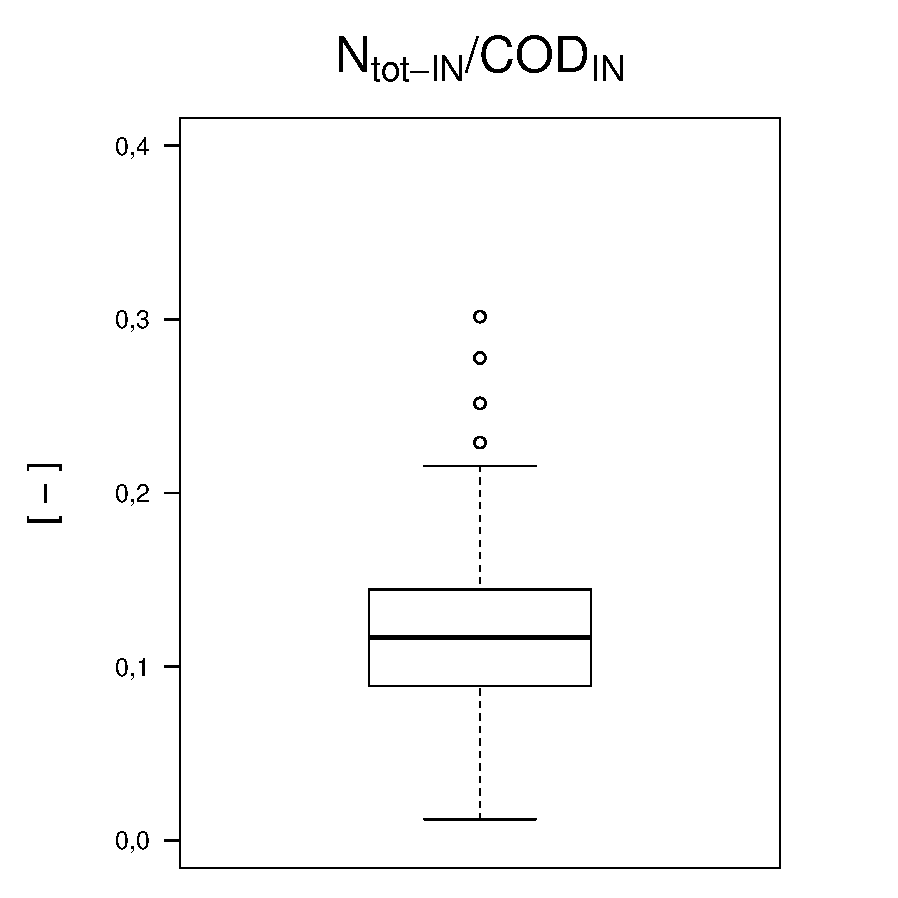
\includegraphics[width=\linewidth]{sa_Ntot_COD}}
	\centering
	\caption{Andamento del rapporto tra azoto totale e COD in ingresso}
	\label{fig:sa_Ntot_COD}
\end{figure}
\begin{figure}[H]
	\fbox{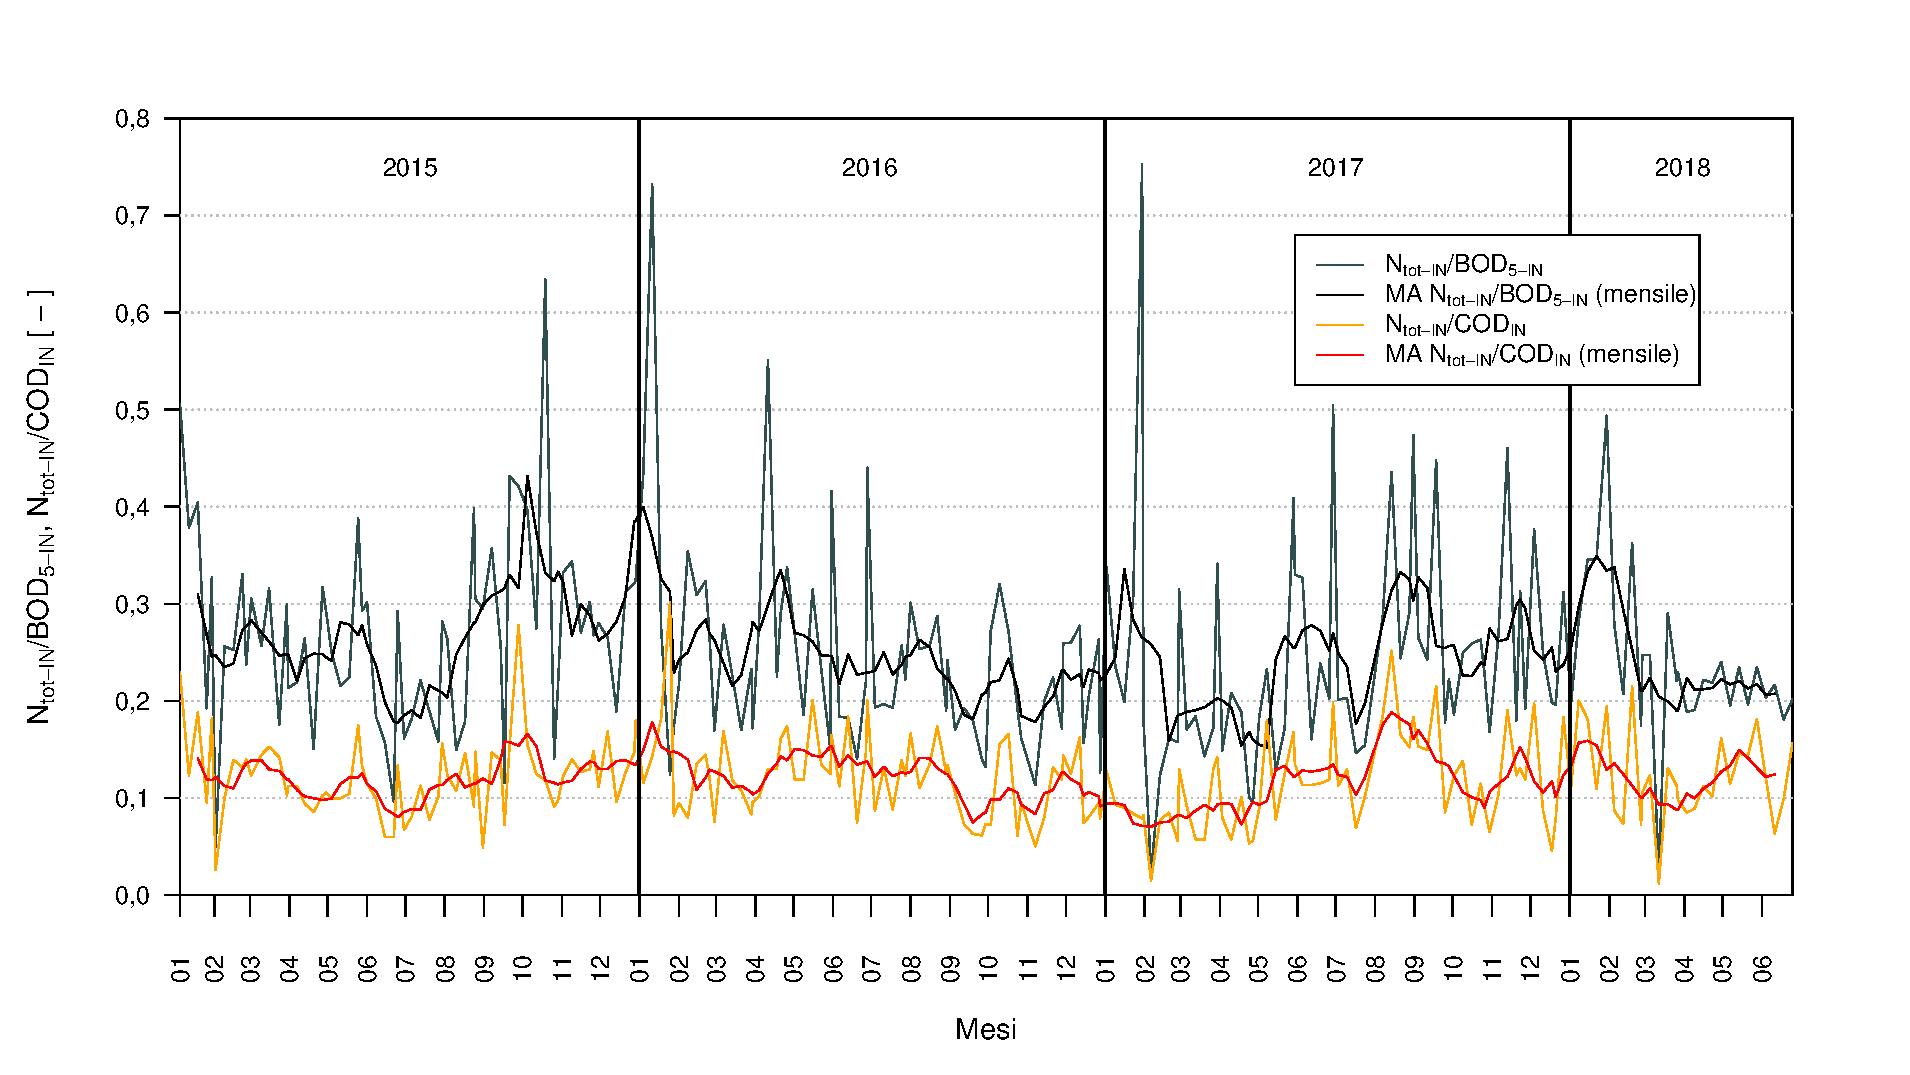
\includegraphics[width=\linewidth]{sa_Ntot_BOD-Ntot_COD}}
	\centering
	\caption{Andamento dei rapporti tra azoto totale e BOD\textsubscript{5} e azoto totale e COD in ingresso}
	\label{fig:sa_Ntot_BOD-Ntot_COD}
\end{figure}
\begin{figure}[H]
	\fbox{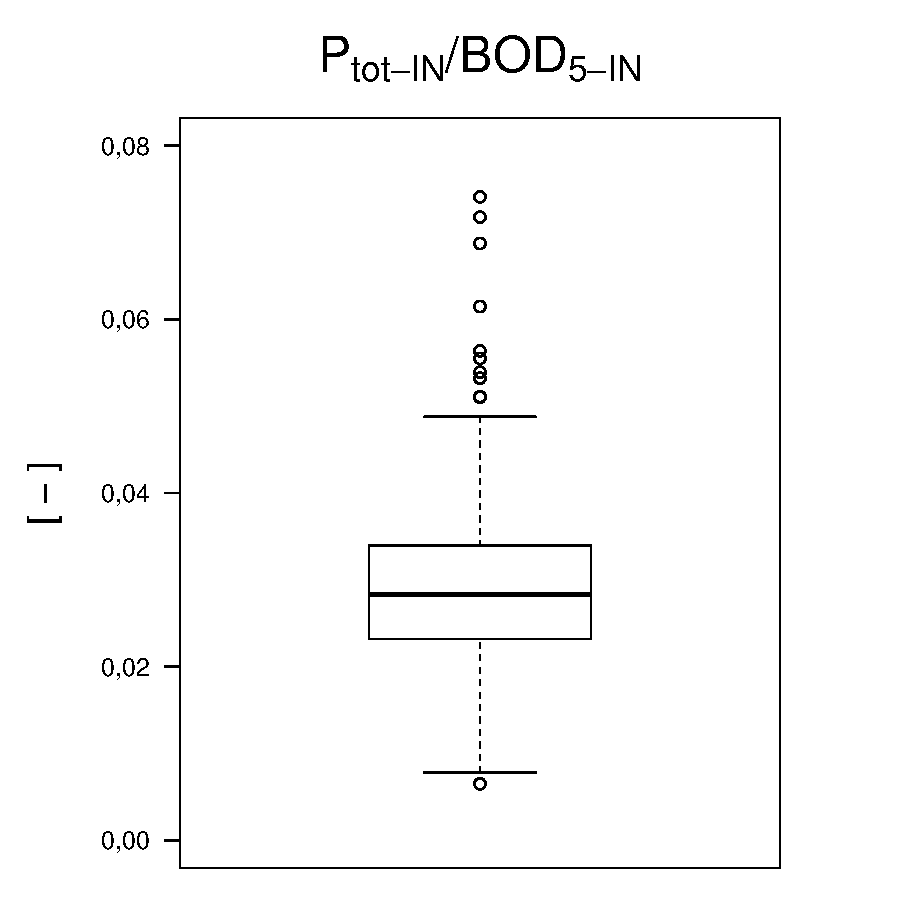
\includegraphics[width=\linewidth]{sa_Ptot_BOD}}
	\centering
	\caption{Andamento del rapporto tra fosforo totale e BOD\textsubscript{5} in ingresso}
	\label{fig:sa_Ptot_BOD}
\end{figure}
\begin{figure}[H]
	\fbox{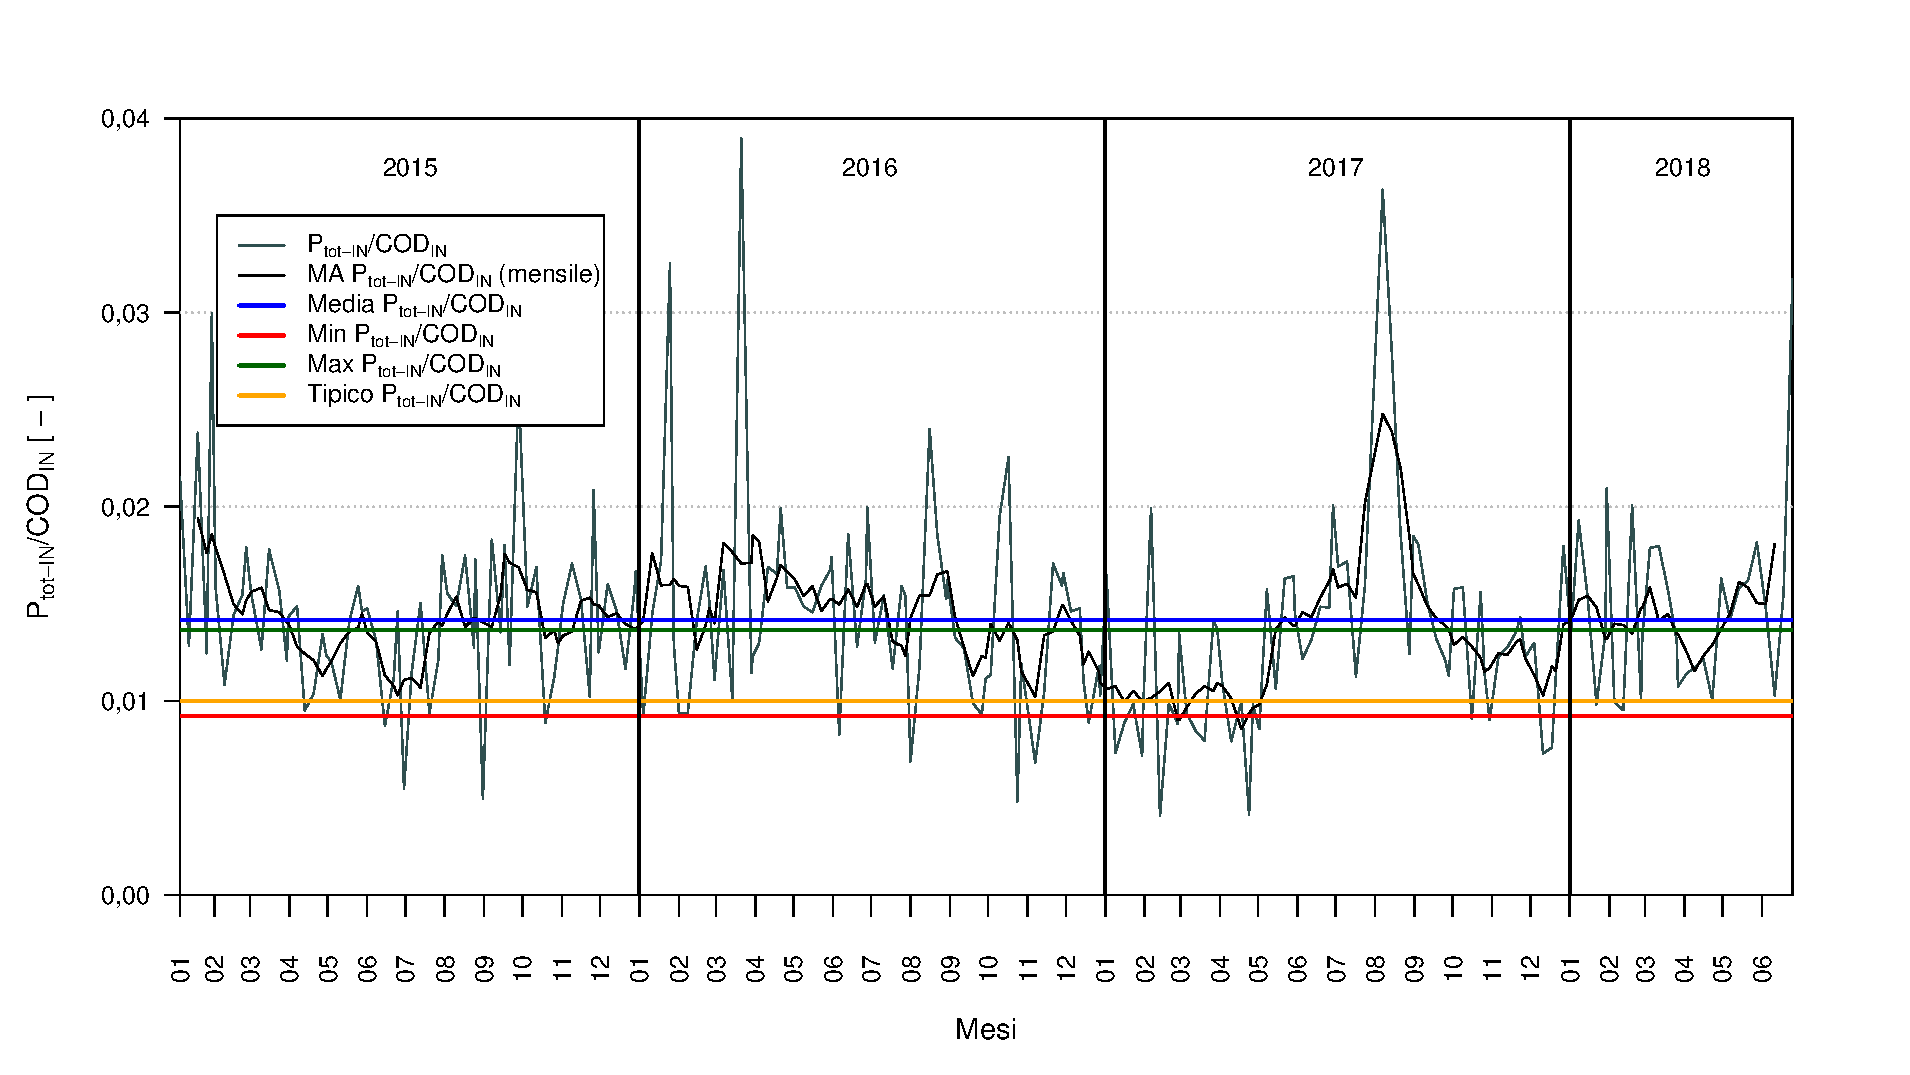
\includegraphics[width=\linewidth]{sa_Ptot_COD}}
	\centering
	\caption{Andamento del rapporto tra fosforo totale e COD in ingresso}
	\label{fig:sa_Ptot_COD}
\end{figure}
\begin{figure}[H]
	\fbox{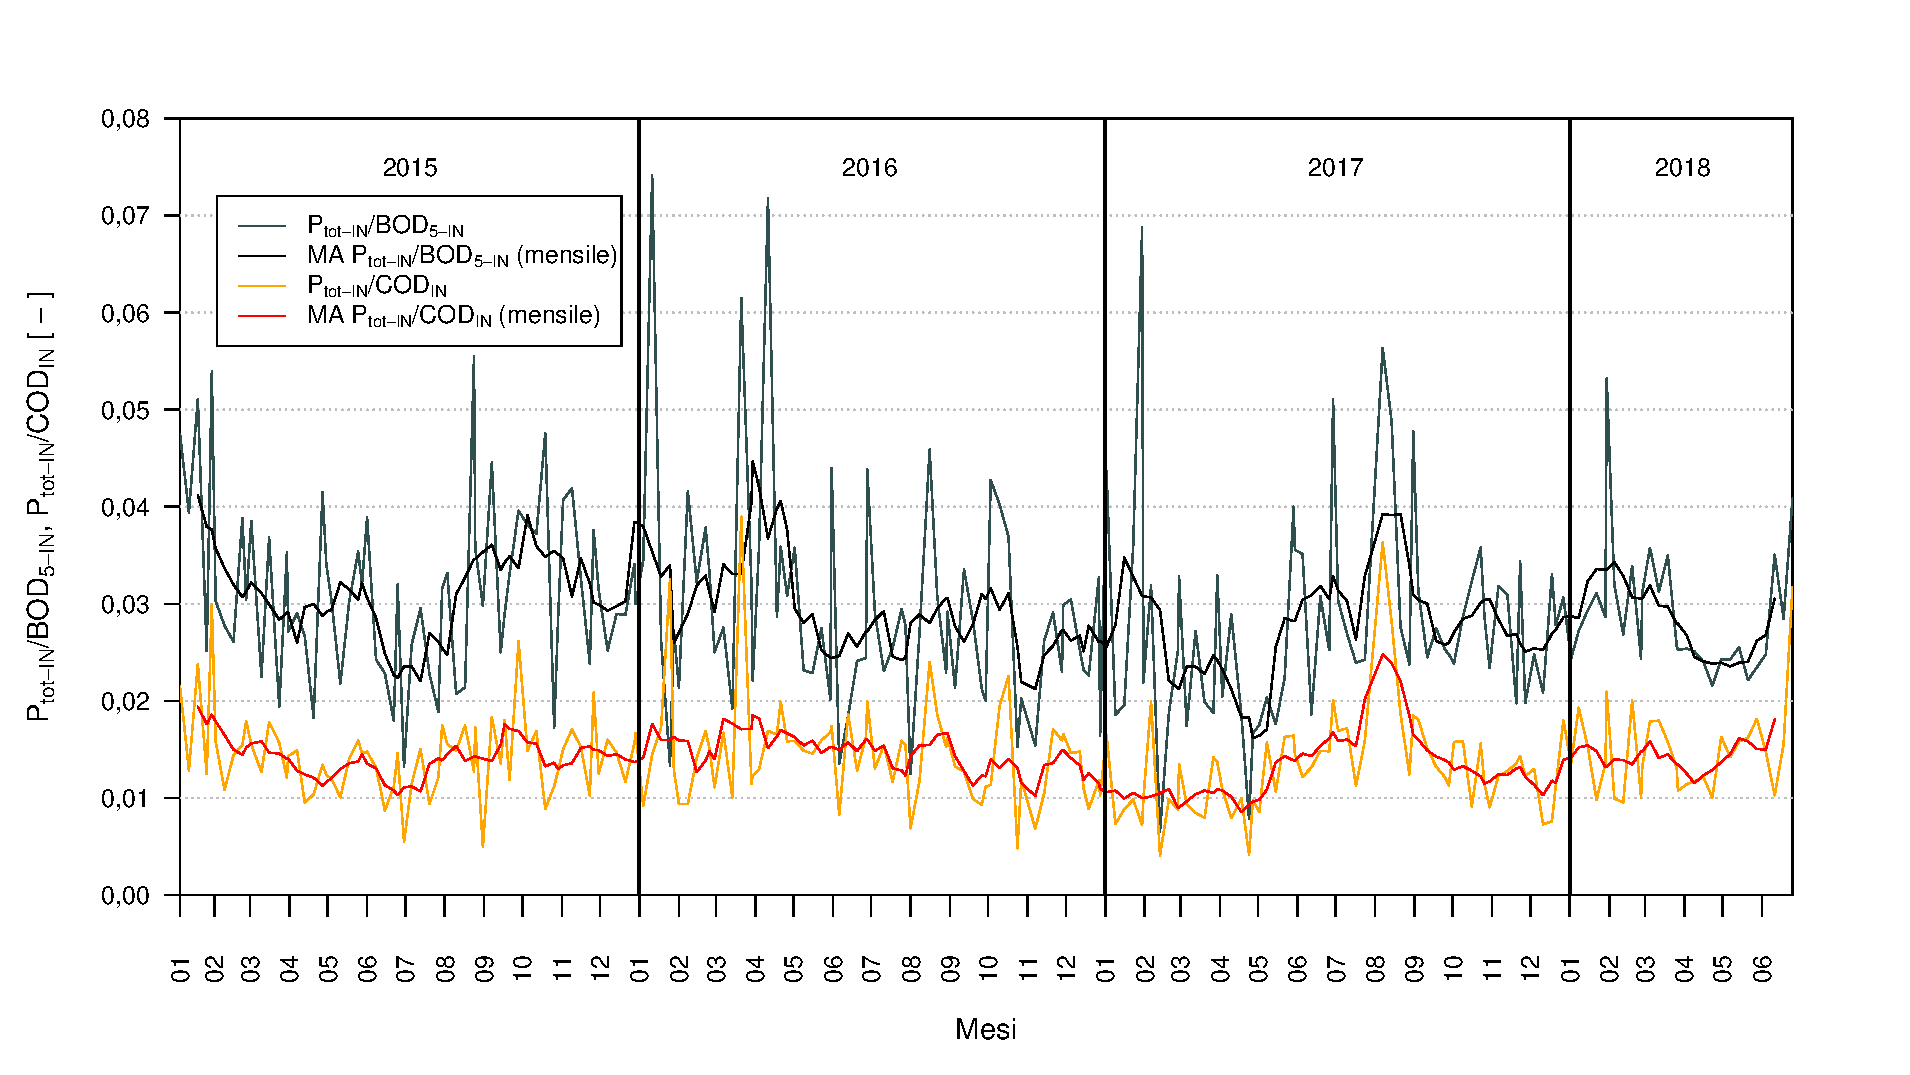
\includegraphics[width=\linewidth]{sa_Ptot_BOD-Ptot_COD}}
	\centering
	\caption{Andamento dei rapporti tra fosforo totale e BOD\textsubscript{5} e fosforo totale e COD in ingresso}
	\label{fig:sa_Ptot_BOD-Ptot_COD}
\end{figure}

Nel confronto del fosforo totale sia con il BOD\textsubscript{5} (\autoref{fig:sa_Ptot_BOD}) che con il COD (\autoref{fig:sa_Ptot_COD}), la media del rapporto eccede il valore massimo per liquami urbani e ciò conferma quanto già osservato in precedenza relativamente alla presenza di scarichi aventi un'altra origine.
Nel grafico di \autoref{fig:sa_Ptot_BOD-Ptot_COD} si vede che questi due rapporti sono correlati.
L’andamento variabile, simile a quello osservato per i rapporti N\textsubscript{tot}/BOD\textsubscript{5} e N\textsubscript{tot}/COD (\autoref{fig:sa_Ntot_BOD-Ntot_COD}), porta alla conclusione che non ci sia però correlazione tra la concentrazione di fosforo e quella di BOD\textsubscript{5} e COD.

\begin{figure}[H]
	\fbox{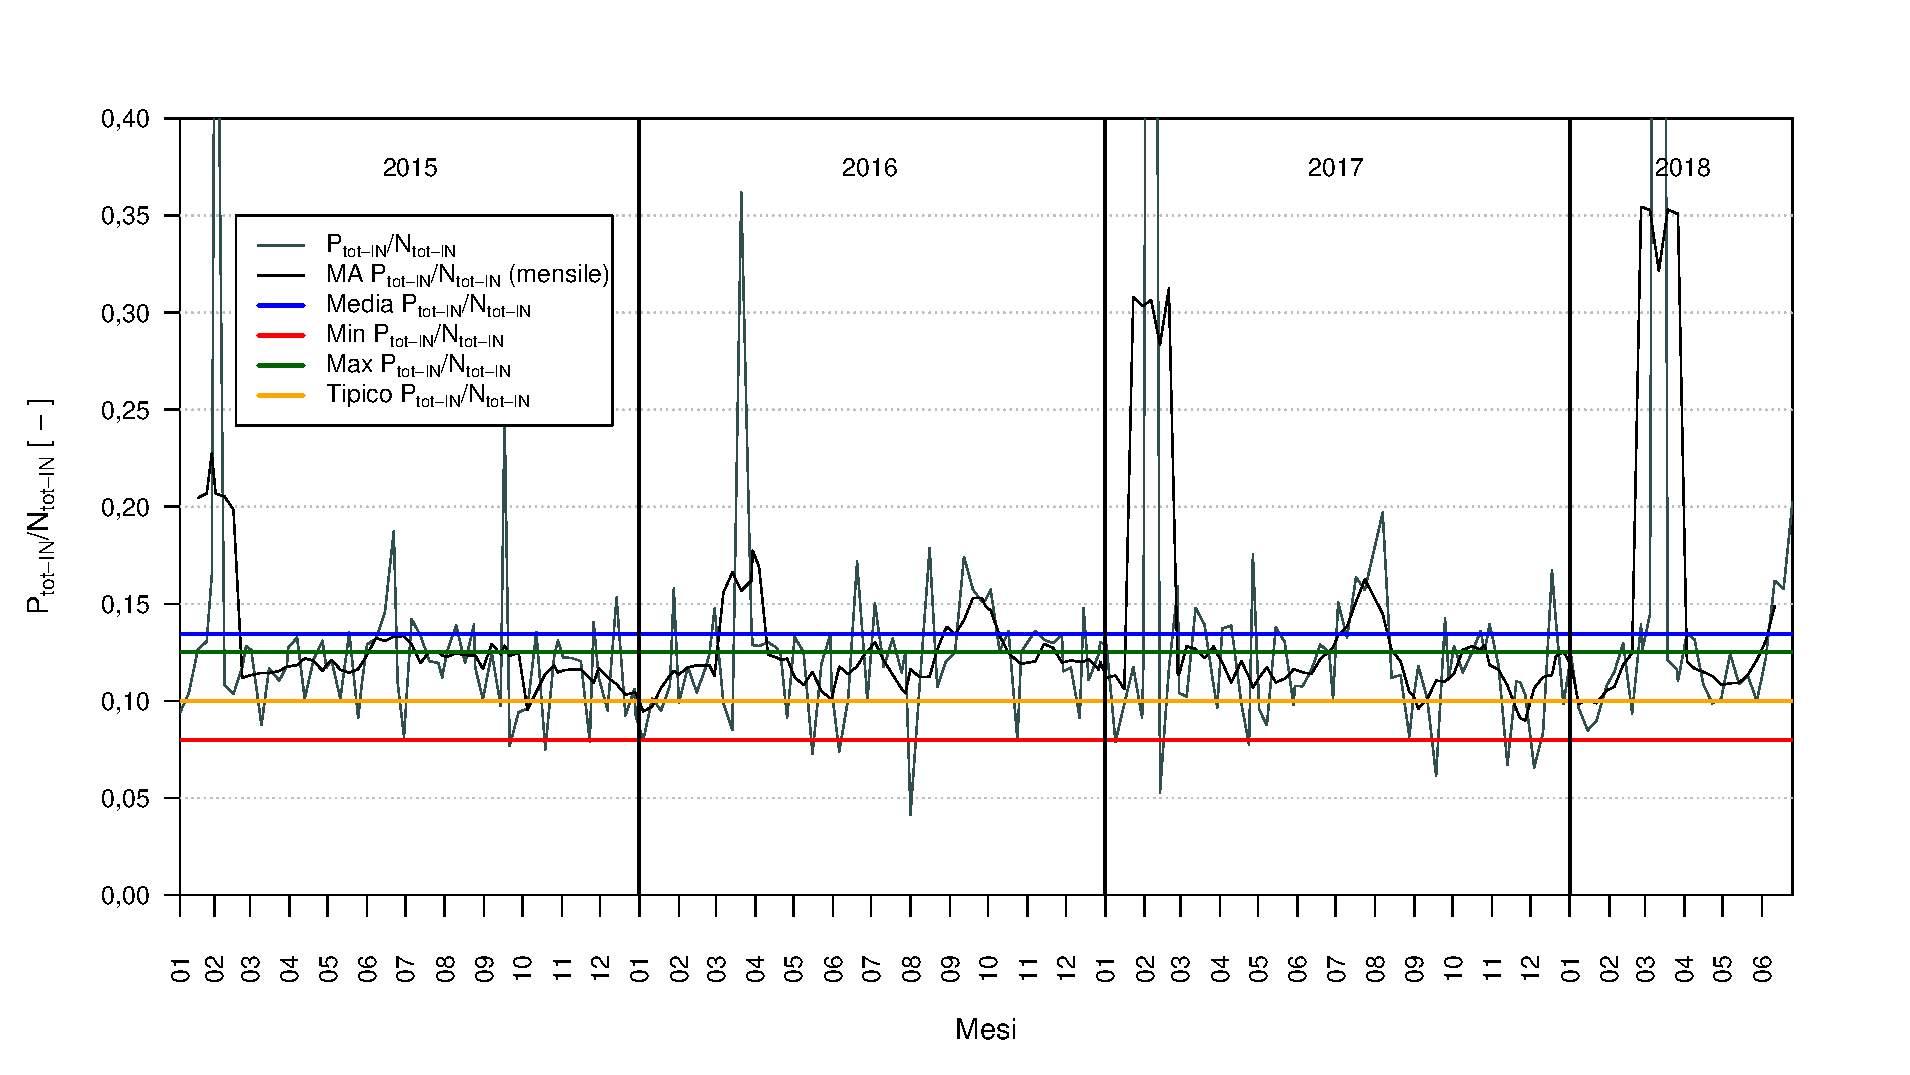
\includegraphics[width=\linewidth]{sa_Ptot_Ntot}}
	\centering
	\caption{Andamento del rapporto tra fosforo totale e azoto totale in ingresso}
	\label{fig:sa_Ptot_Ntot}
\end{figure}

L’andamento del rapporto tra fosforo totale e azoto totale in ingresso all’impianto di depurazione è riportato in \autoref{fig:sa_Ptot_Ntot}.
Ad eccezione di alcuni valori estremi, tale rapporto ha un andamento pressappoco stabile, con media che supera il valore massimo atteso per un liquame urbano.
\begin{table}[H]
	\begin{center}
		\scriptsize
		\begin{tabular}{|>{\centering\arraybackslash}p{3cm}|>{\centering\arraybackslash}p{3cm}|>{\centering\arraybackslash}p{3cm}|}
			\hline 
			\textbf{Rapporto} & \textbf{Media} & \textbf{Valore tipico} \\ 
			\hline 
			BOD\textsubscript{5}/COD & 0,50 & 0,50 \\ 
			\hline 
			N\textsubscript{tot}/BOD\textsubscript{5} & 0,25 & 0,20 \\ 
			\hline 
			N\textsubscript{tot}/COD & 0,12 & 0,10 \\ 
			\hline 
			P\textsubscript{tot}/BOD & 0,029 & 0,020 \\ 
			\hline 
			P\textsubscript{tot}/COD & 0,014 & 0,010 \\ 
			\hline 
			P\textsubscript{tot}/N\textsubscript{tot} & 0,13 & 0,10 \\ 
			\hline 
		\end{tabular} 
		\caption{Valori medi calcolati e  valori tipici per un liquame urbano dei rapporti significativi tra le concentrazioni di inquinanti in ingresso}
		\label{tab:sa_rapporti}
	\end{center}	
\end{table}	
In \autoref{tab:sa_rapporti} sono raccolti i valori medi dei rapporti calcolati e i rispettivi valori tipici per liquami urbani. Si osserva che le caratteristiche del liquame sono sbilanciate verso i nutrienti e in particolare verso il fosforo.\\

\begin{figure}
	\fbox{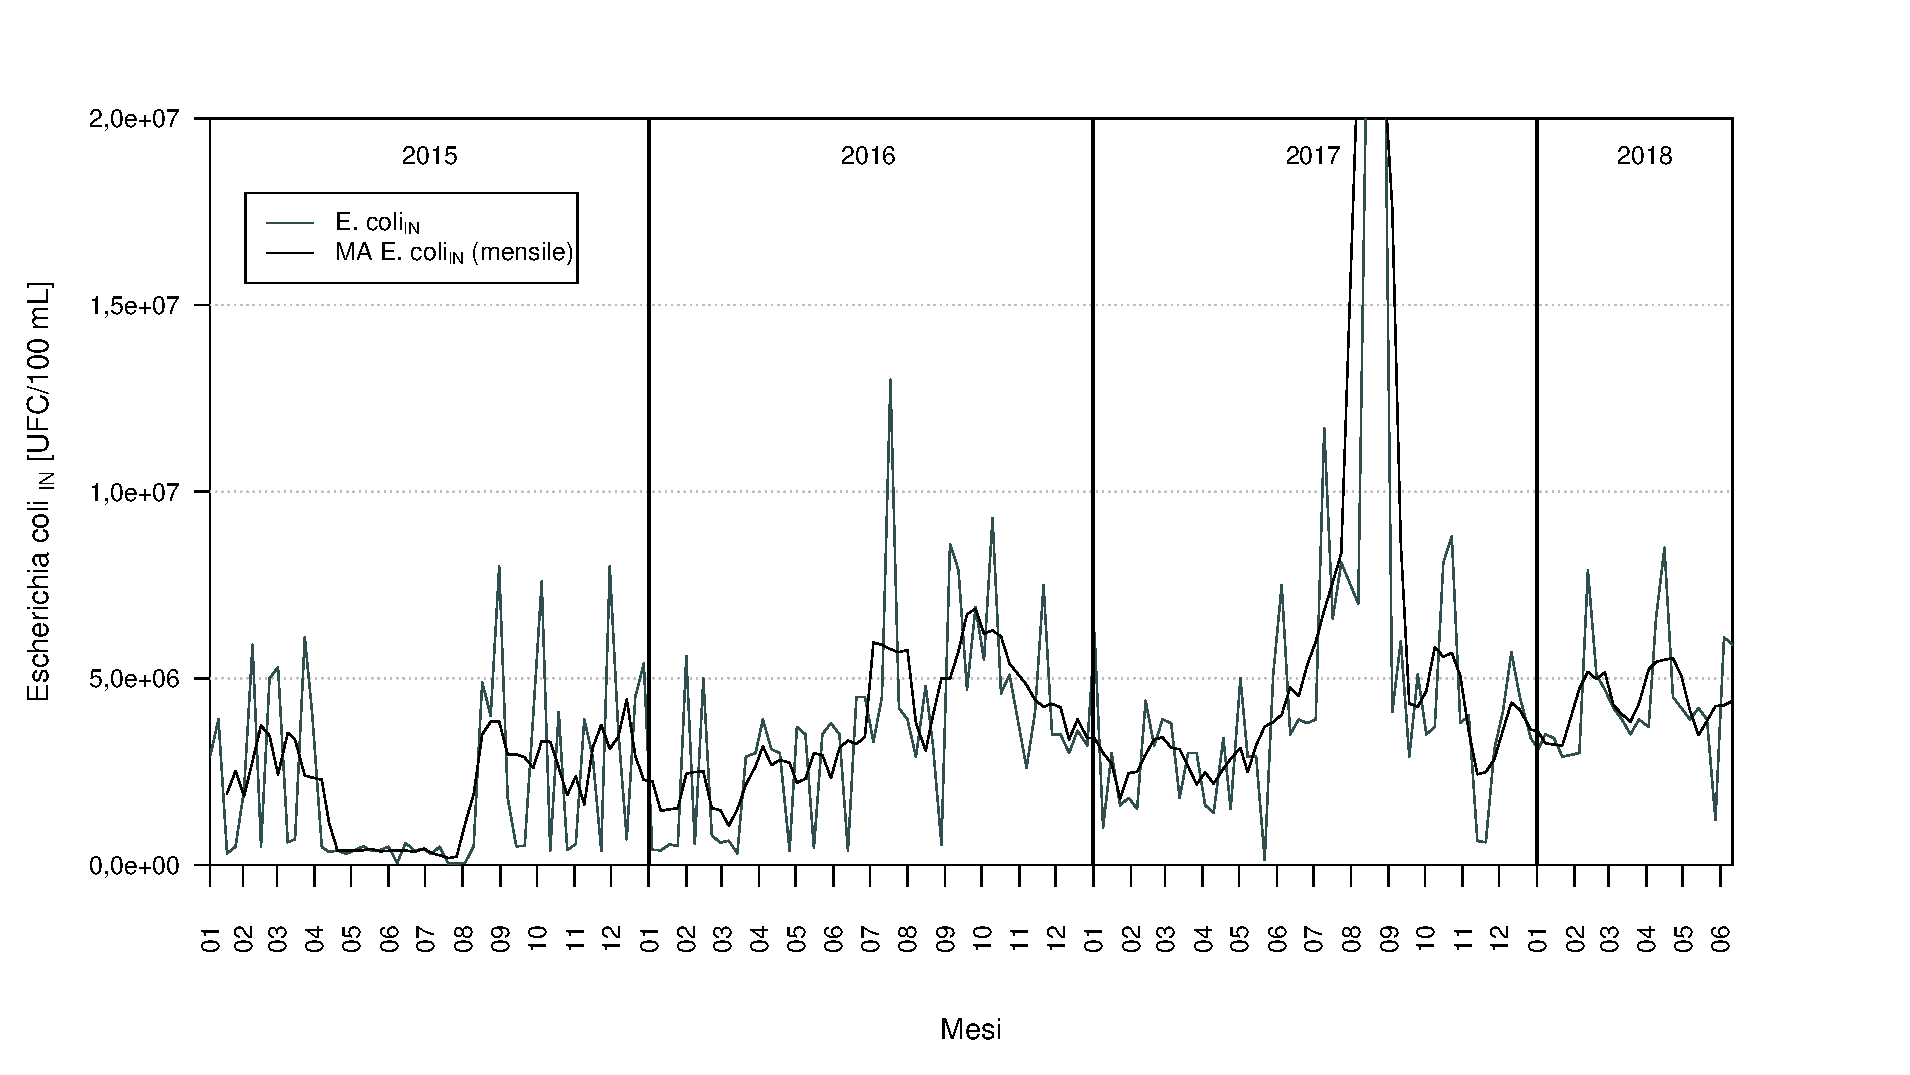
\includegraphics[width=\linewidth]{sa_EC}}
	\centering
	\caption{Andamento della concentrazione in ingresso di \textit{Escherichia coli}}
	\label{fig:sa_EC}
\end{figure}

La concentrazione di carica batterica in termini di \textit{Escherichia coli} è rappresentata in \autoref{fig:sa_EC}. Si nota una certa variabilità e sembra si manifesti un trend leggermente crescente.

\begin{figure}
	\fbox{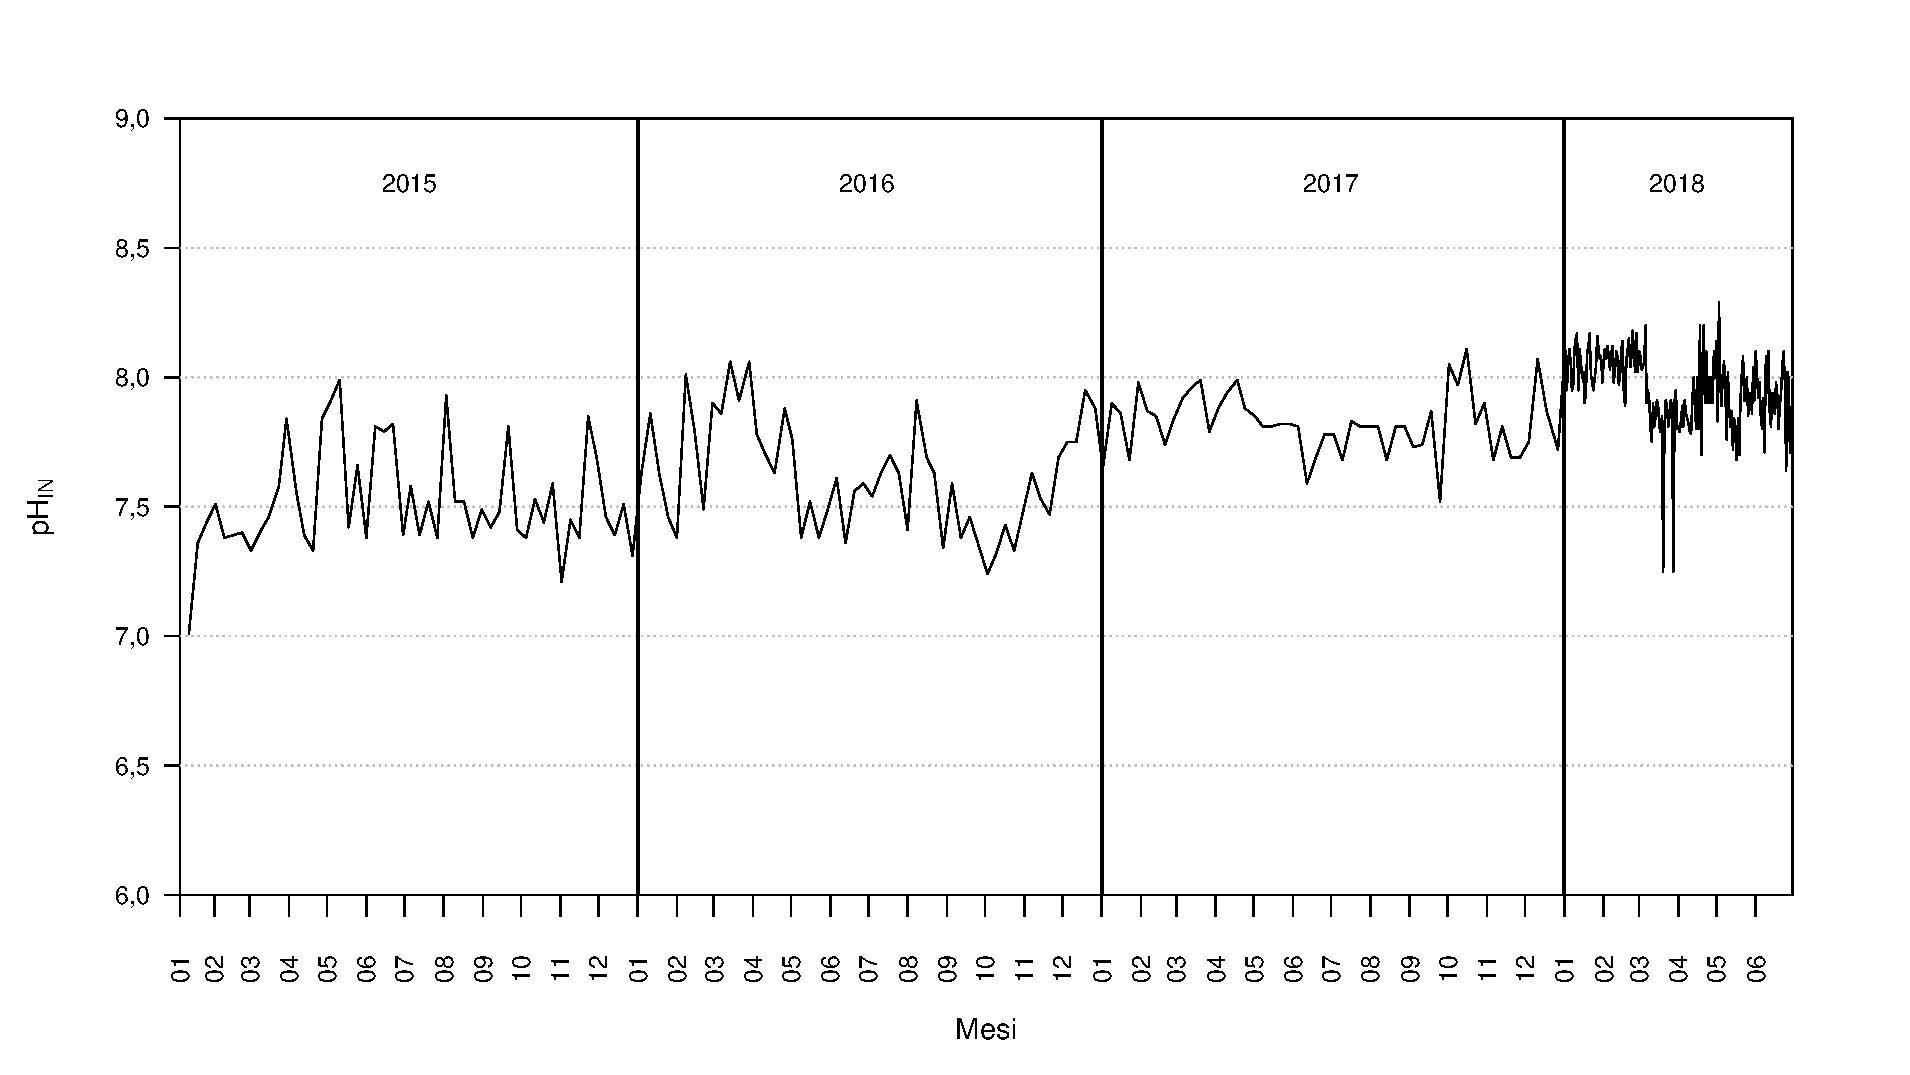
\includegraphics[width=\linewidth]{sa_pH}}
	\centering
	\caption{Andamento del pH del liquame in ingresso}
	\label{fig:sa_pH}
\end{figure}




Il grafico di \autoref{fig:sa_pH} riporta l’andamento del pH del liquame in ingresso.
Nel caso in esame, il valore medio è pari a 7,7 e, in alcuni periodi, si supera il valore 8. Questo comportamento potrebbe derivare da variazioni delle caratteristiche degli scarichi non domestici in fognatura. A partire dalla seconda metà del 2016, si nota un trend crescente.

\begin{figure}
	\fbox{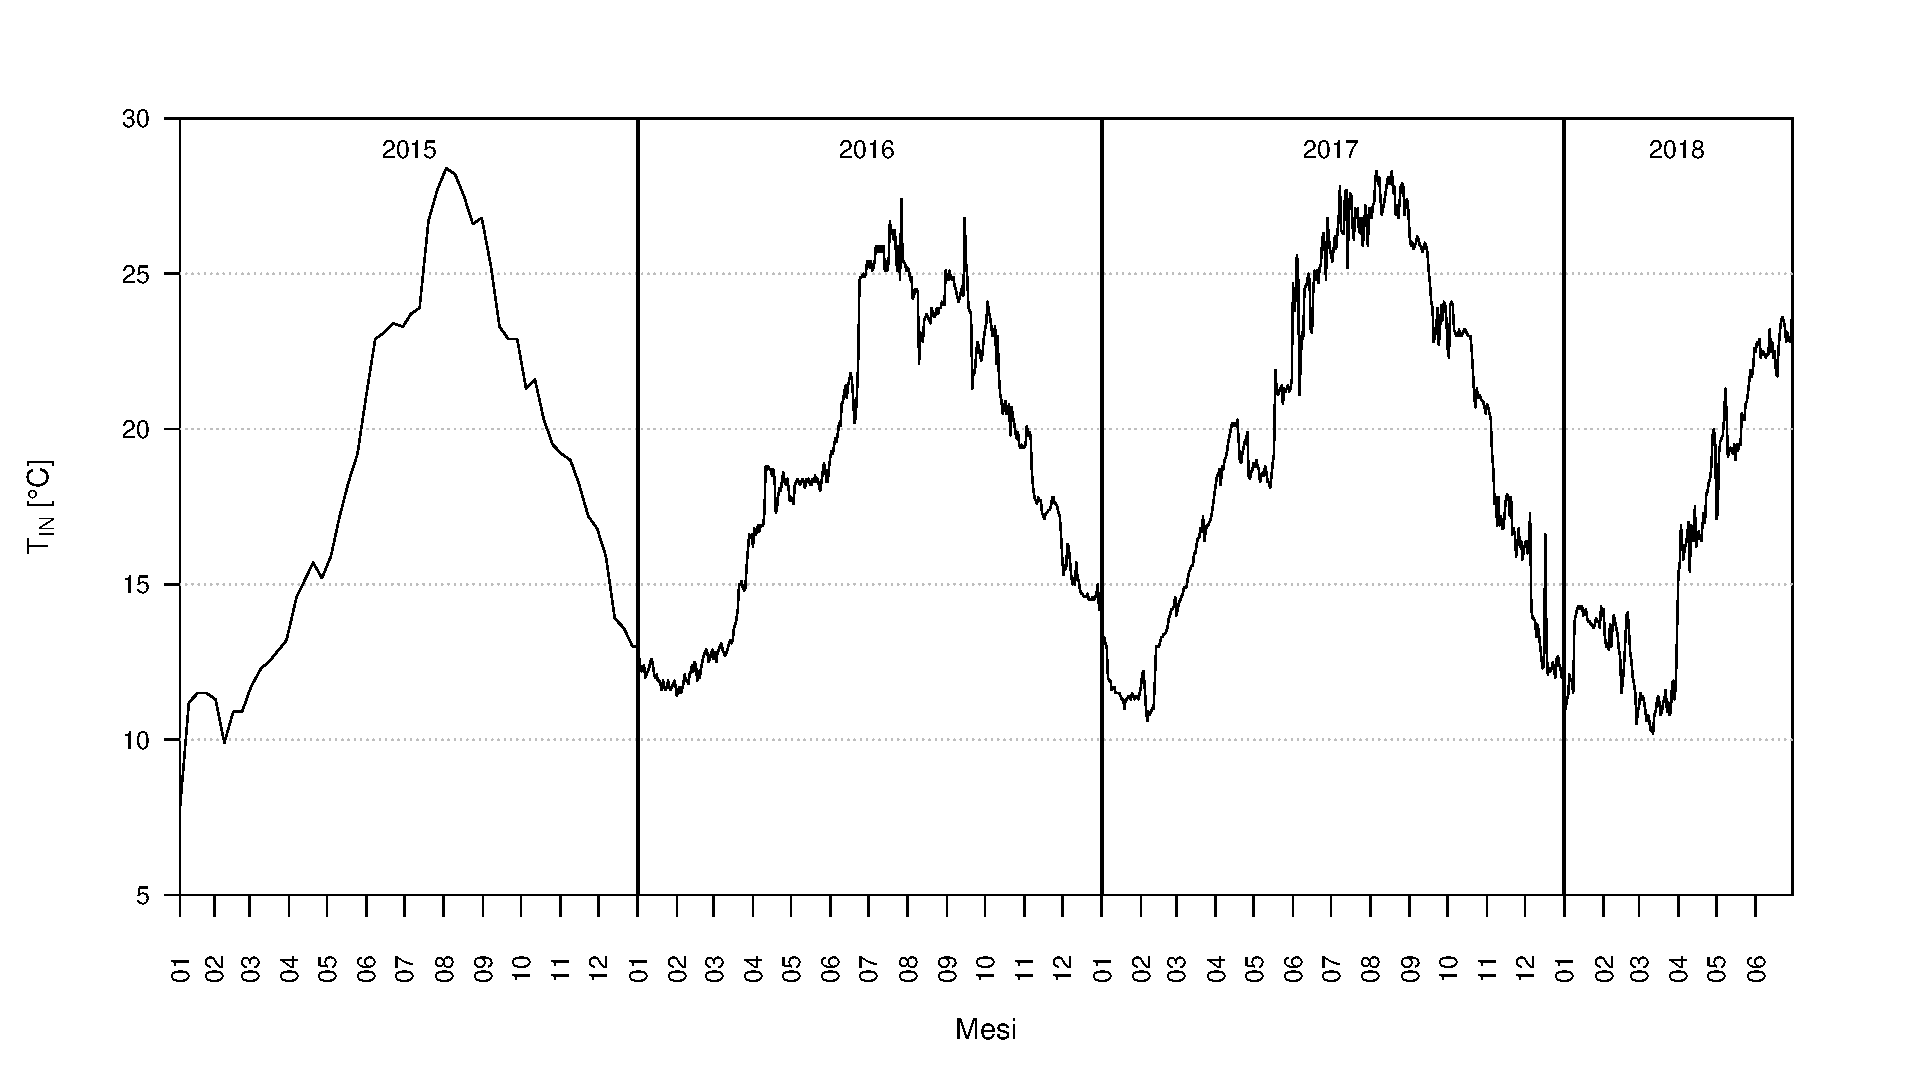
\includegraphics[width=\linewidth]{sa_T}}
	\centering
	\caption{Andamento della temperatura del liquame in ingresso}
	\label{fig:sa_T}
\end{figure}

Le oscillazioni della temperatura del refluo in ingresso ricalcano l’andamento previsto dall’alternarsi delle stagioni dell’anno (\autoref{fig:sa_T}).
Si osservano valori minimi di poco superiori ai 10\textdegree C e valori massimi attorno ai 26-28\textdegree C.

\paragraph{Carichi inquinanti}

A partire dai dati di concentrazione e da quelli di portata è stato possibile calcolare i carichi degli inquinanti in ingresso all'impianto (per il calcolo, si veda la \autoref{subsec:carichi}).

L'andamento dei carichi di BOD\textsubscript{5} e di COD (\autoref{fig:sa_car_BOD} e \autoref{fig:sa_COD_T}) presenta un tratto decrescente in corrispondenza dell'anno 2015, come si osservava anche per la portata, ma attenuato dall'assenza di trend per le concentrazioni di BOD\textsubscript{5} e COD. Risulta esserci, inoltre, una certa corrispondenza tra picchi di concentrazione e picchi di carico.
Si nota che i carichi di COD e di BOD\textsubscript{5} assumono valori più bassi nei periodi estivi, ovvero quando le temperature sono più alte, e aumentano, invece, quando le temperature si abbassano.
\begin{figure}[H]
	\fbox{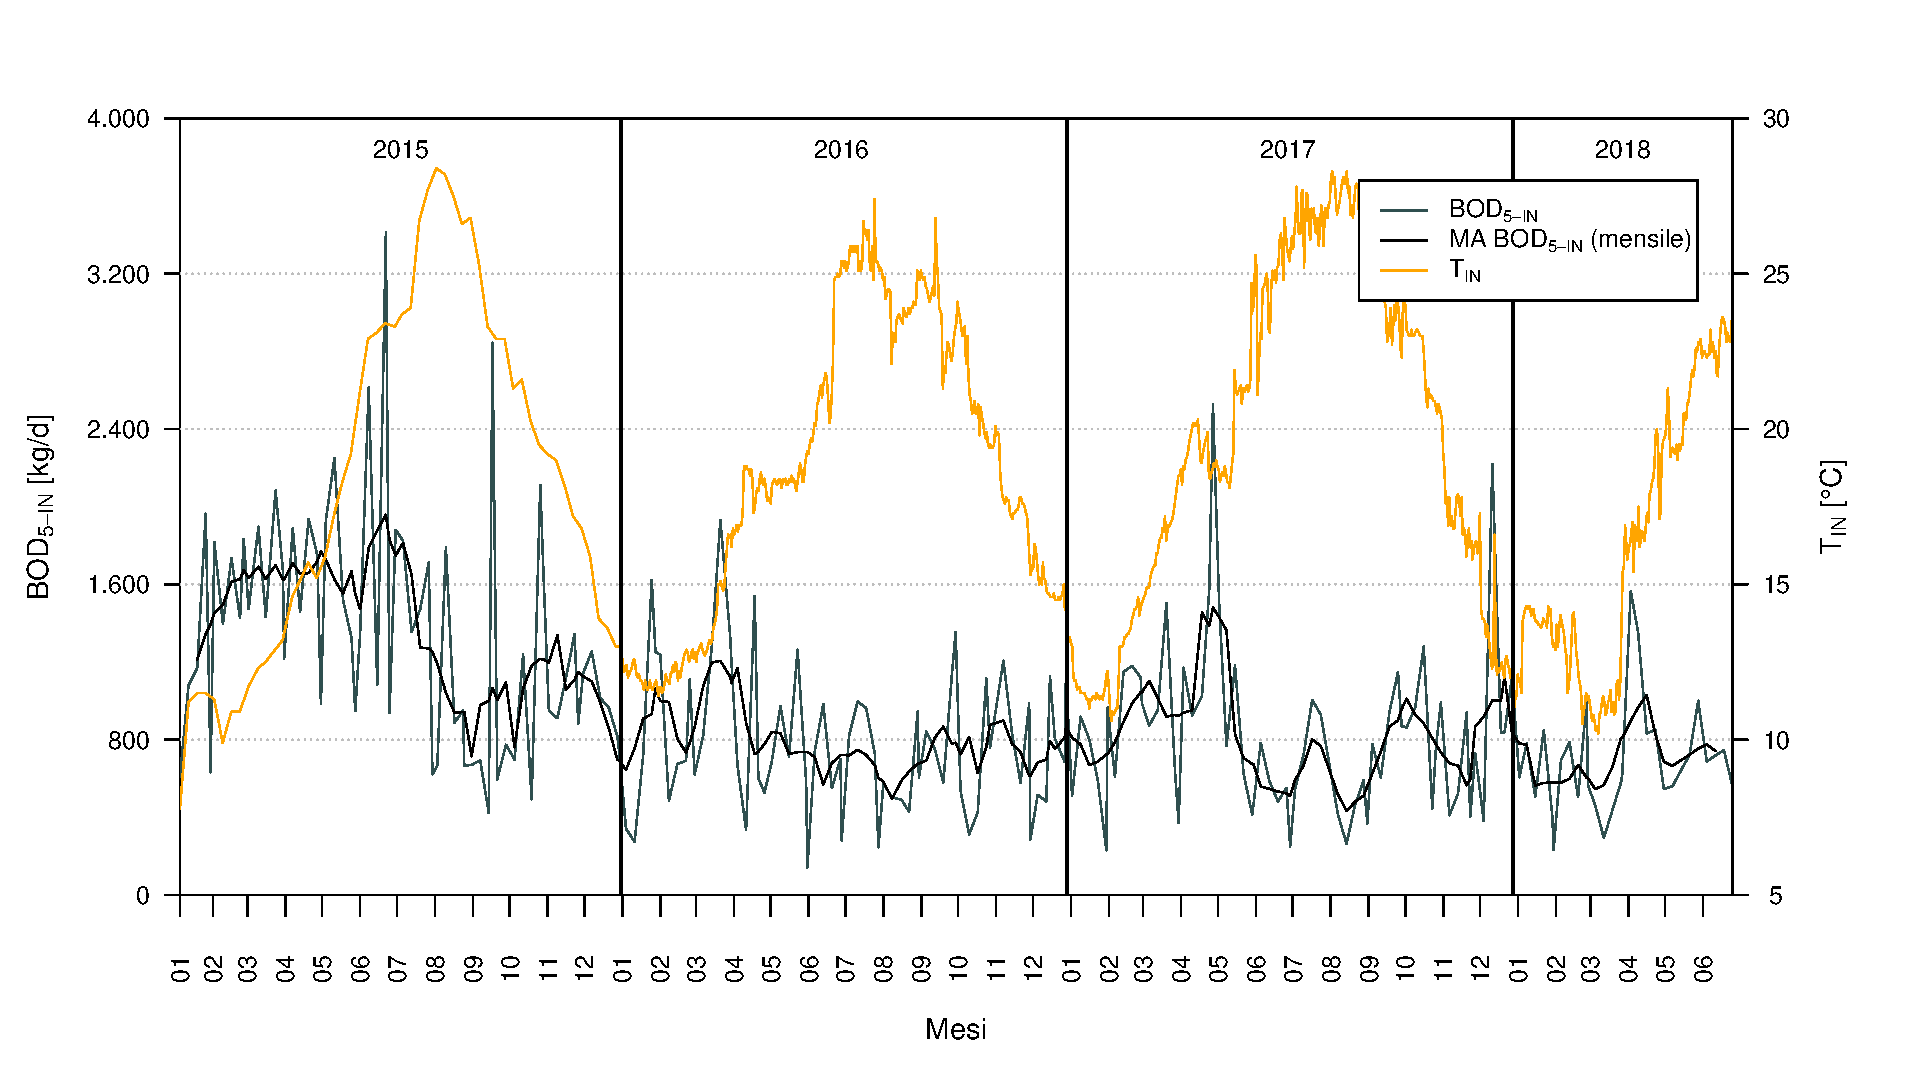
\includegraphics[width=\linewidth]{sa_car_BOD}}
	\centering
	\caption{Andamento del carico in ingresso di BOD\textsubscript{5} e della temperatura del liquame in ingresso}
	\label{fig:sa_car_BOD}
\end{figure}
\begin{figure}[H]
	\fbox{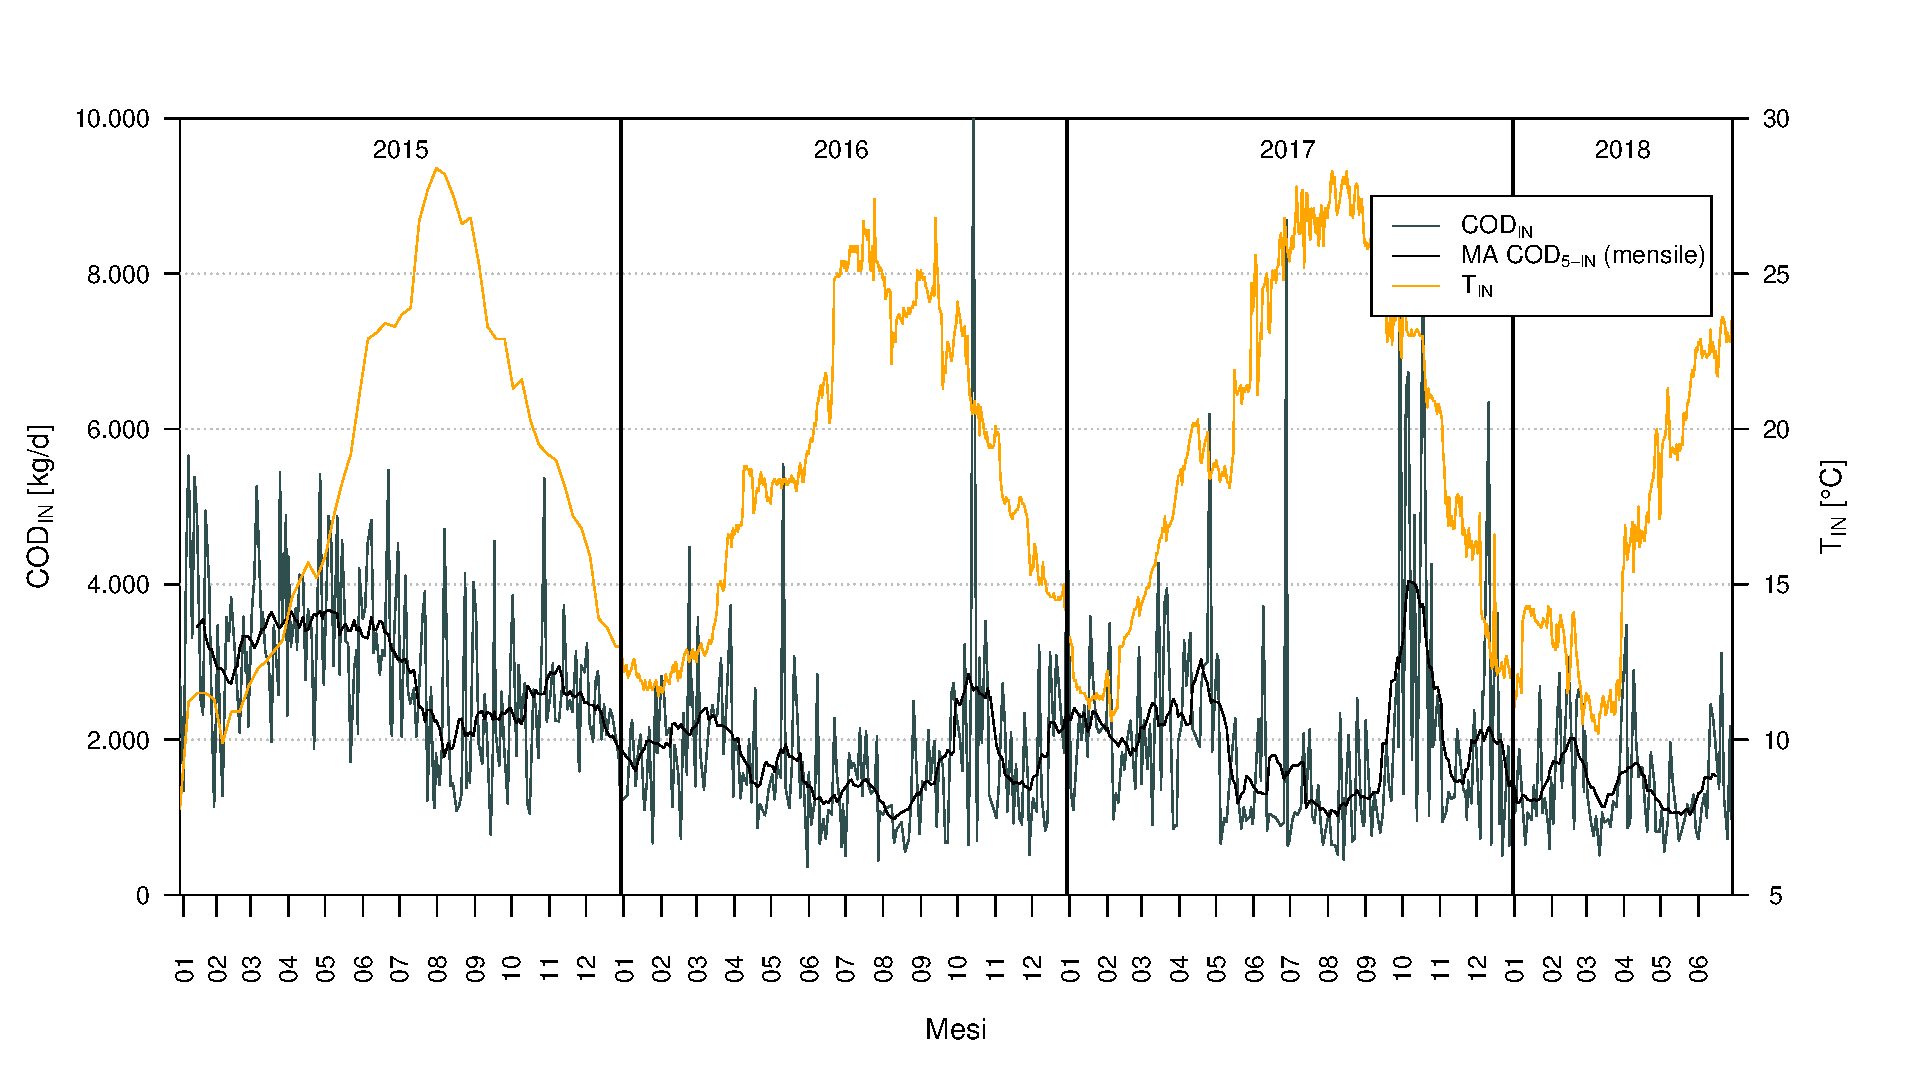
\includegraphics[width=\linewidth]{sa_COD_T}}
	\centering
	\caption{Andamento del carico in ingresso di COD e della temperatura del liquame in ingresso}
	\label{fig:sa_COD_T}
\end{figure}
La \autoref{fig:sa_CODsup} mostra la distribuzione di frequenza dei carichi di COD e di BOD\textsubscript{5} e i percentili 90°, 75° e 50° considerando il periodo complessivo 2015 - 2018. Se, invece, si esclude l'anno 2015 (poiché, coma già spiegato, ha un comportamento anomalo), la distribuzione di frequenza diventa quella di \autoref{fig:sa_CODsupno2015}.
\begin{figure}[H]
	\fbox{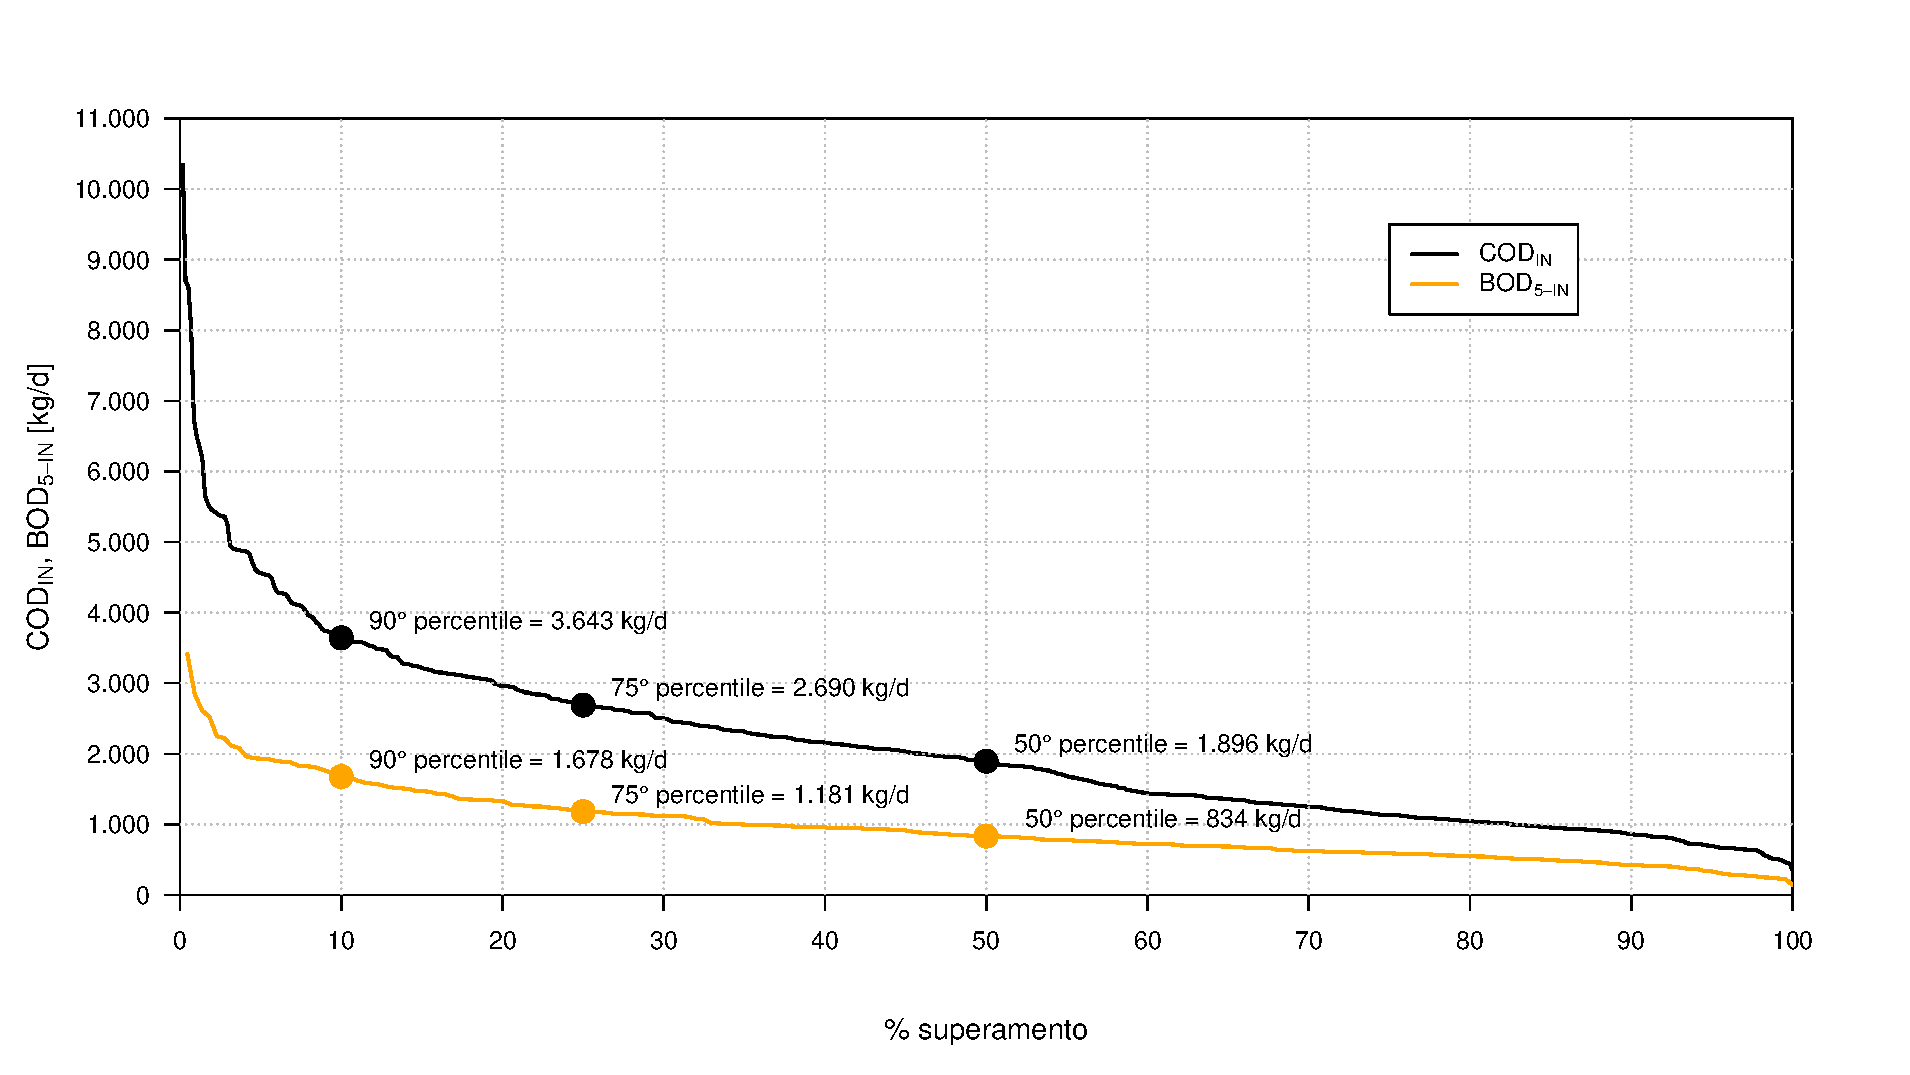
\includegraphics[width=\linewidth]{sa_CODsup}}
	\centering
	\caption{Distribuzione di frequenza dei carichi giornalieri in ingresso di COD e di BOD\textsubscript{5}, periodo 2015 - 2018}
	\label{fig:sa_CODsup}
\end{figure}
\begin{figure}[H]
	\fbox{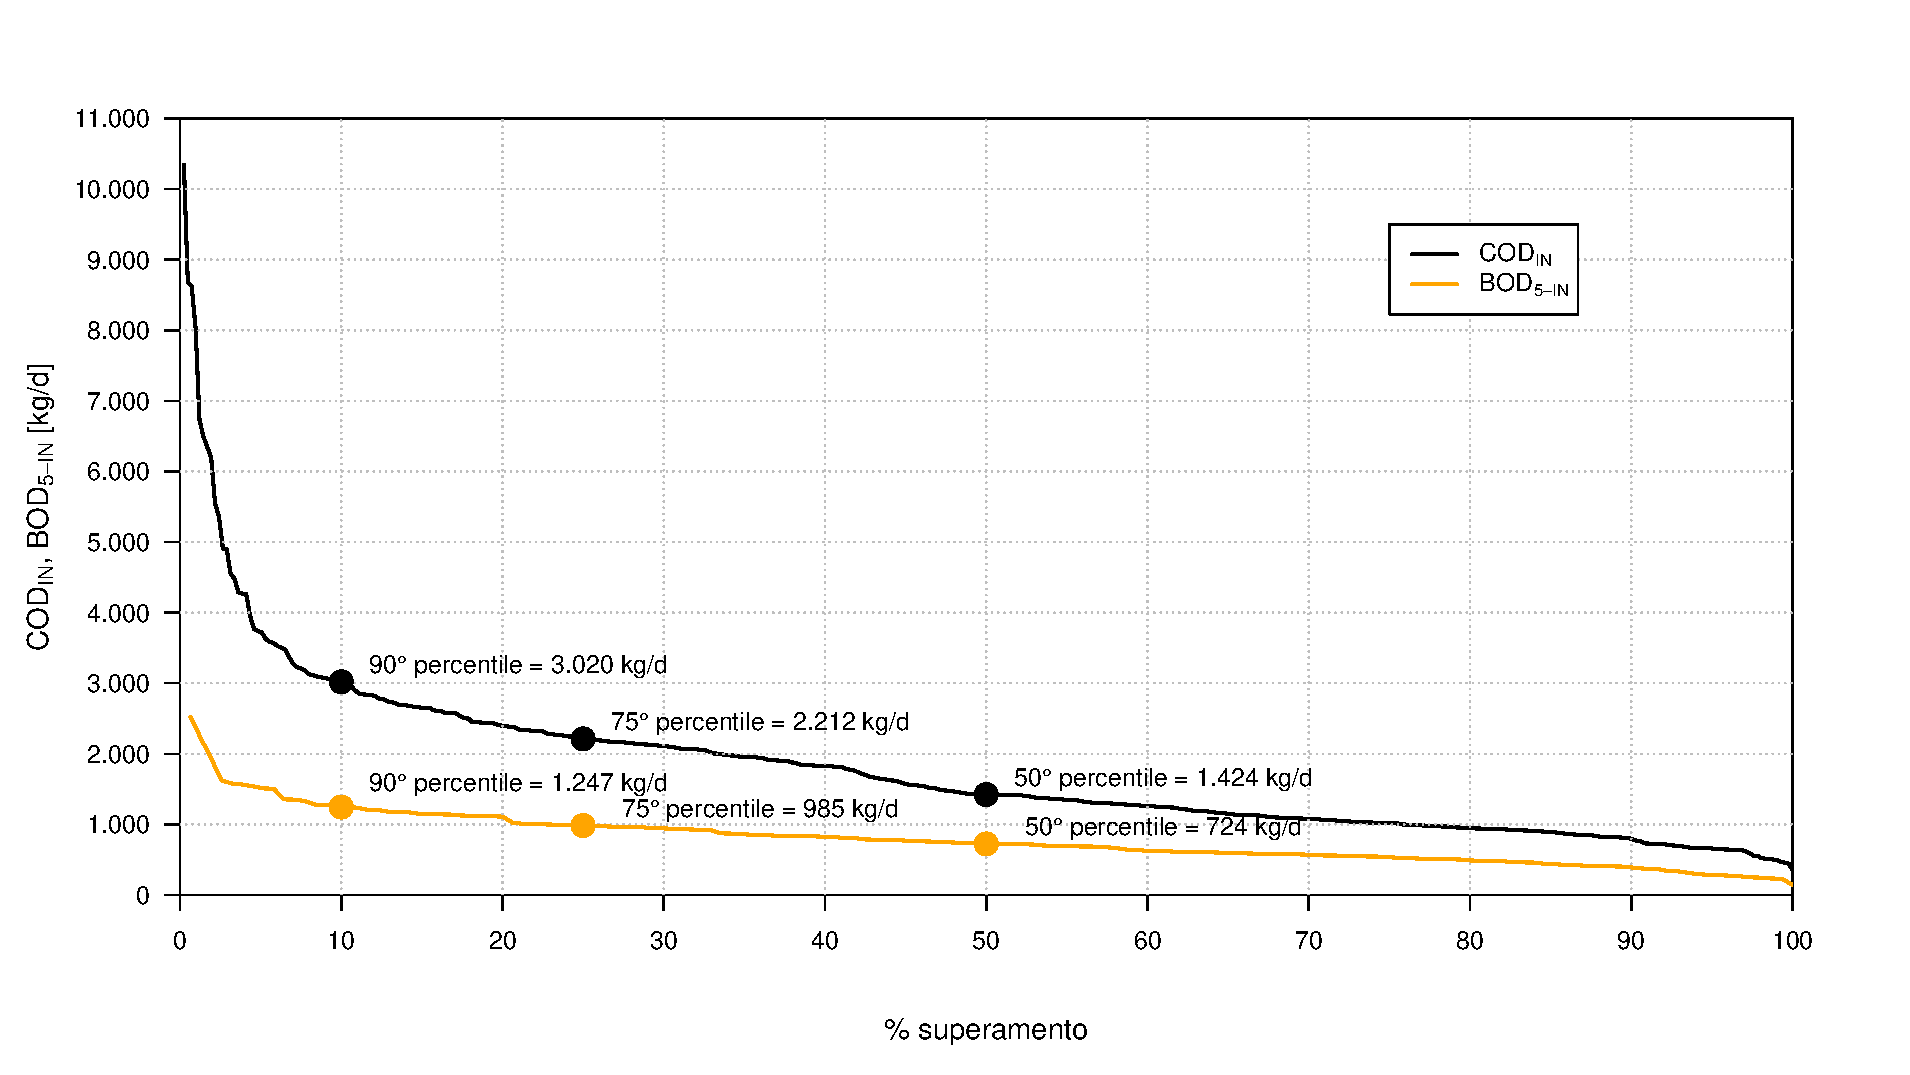
\includegraphics[width=\linewidth]{sa_CODsupno2015}}
	\centering
	\caption{Distribuzione di frequenza dei carichi giornalieri in ingresso di COD e di BOD\textsubscript{5}, periodo 2016 - 2018}
	\label{fig:sa_CODsupno2015}
\end{figure}
\begin{figure}[H]
	\fbox{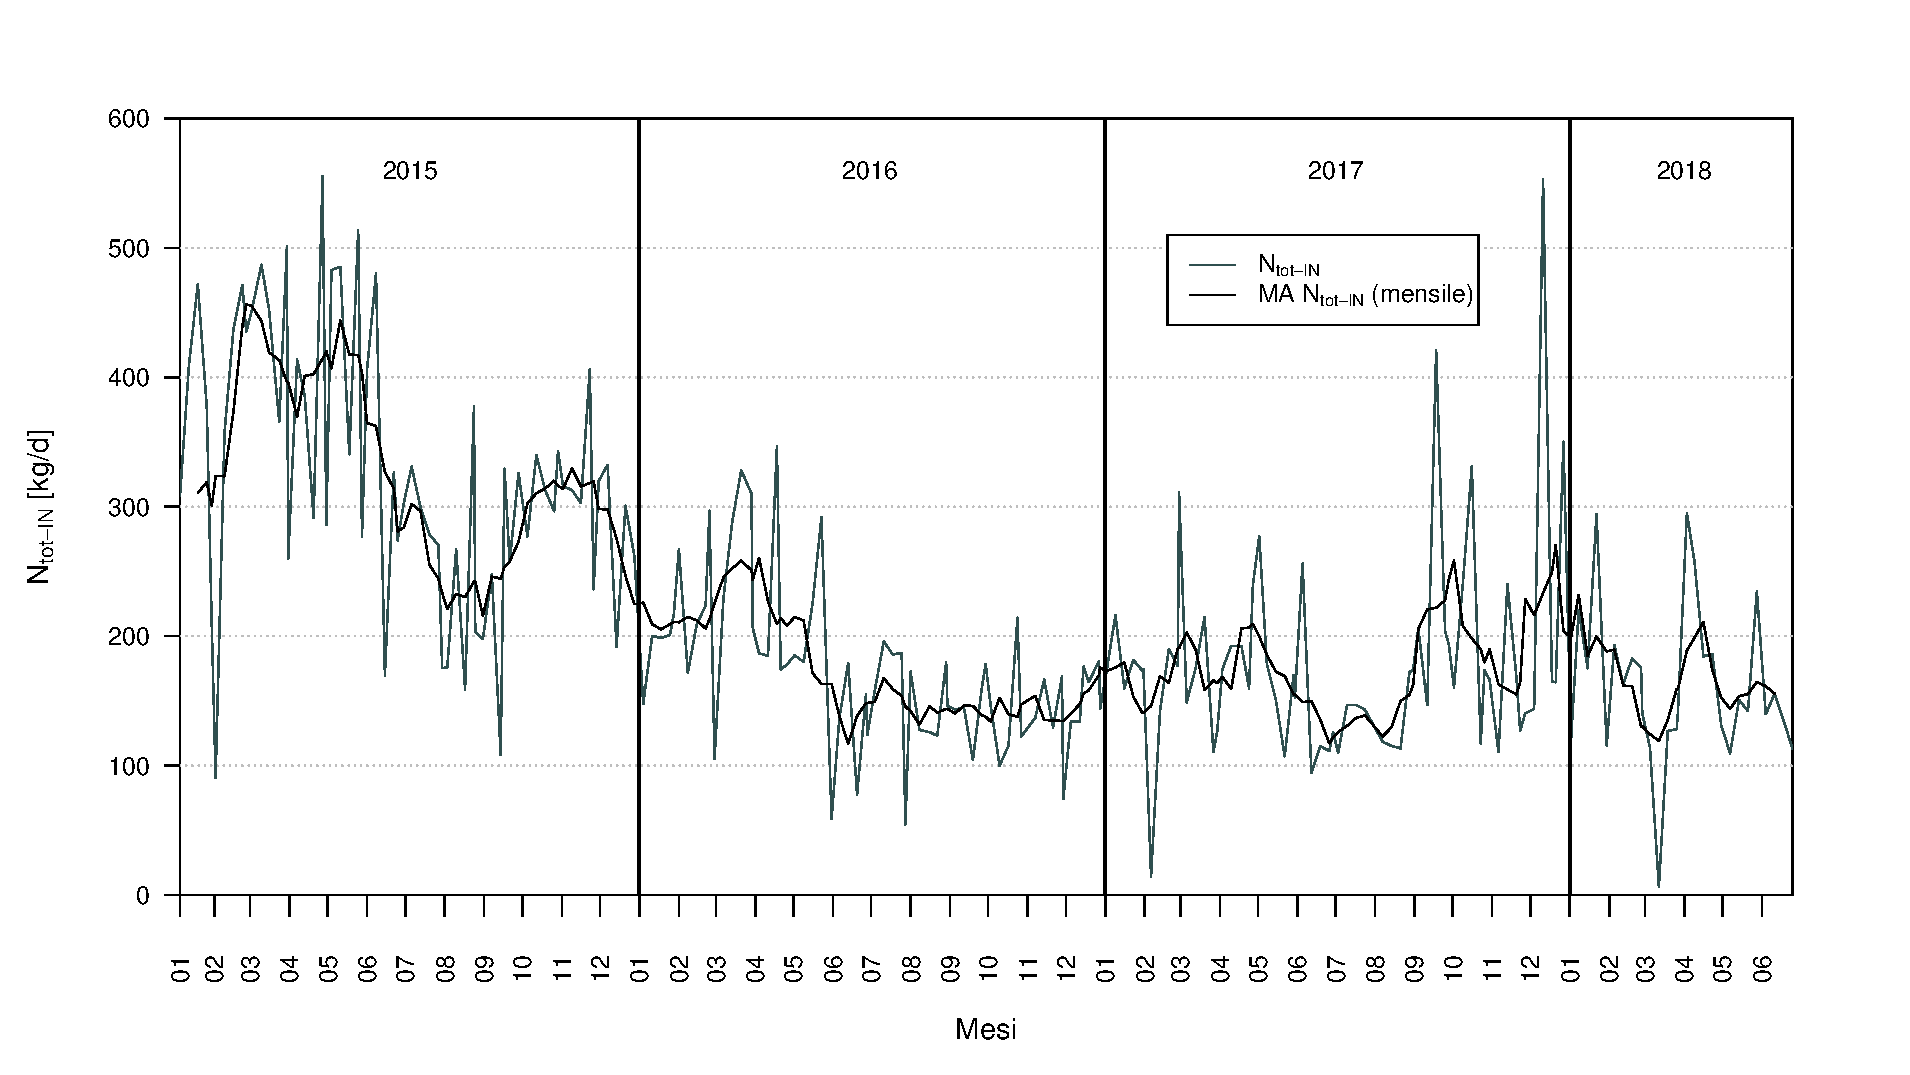
\includegraphics[width=\linewidth]{sa_car_Ntot}}
	\centering
	\caption{Andamento del carico in ingresso di azoto totale}
	\label{fig:sa_car_Ntot}
\end{figure}

Il carico di azoto totale e quello di fosforo totale esibiscono un andamento marcatamente decrescente fino a metà 2016 mentre, successivamente, si assestano (\autoref{fig:sa_car_Ntot} e \autoref{fig:sa_car_Ptot}).

\begin{figure}[H]
	\fbox{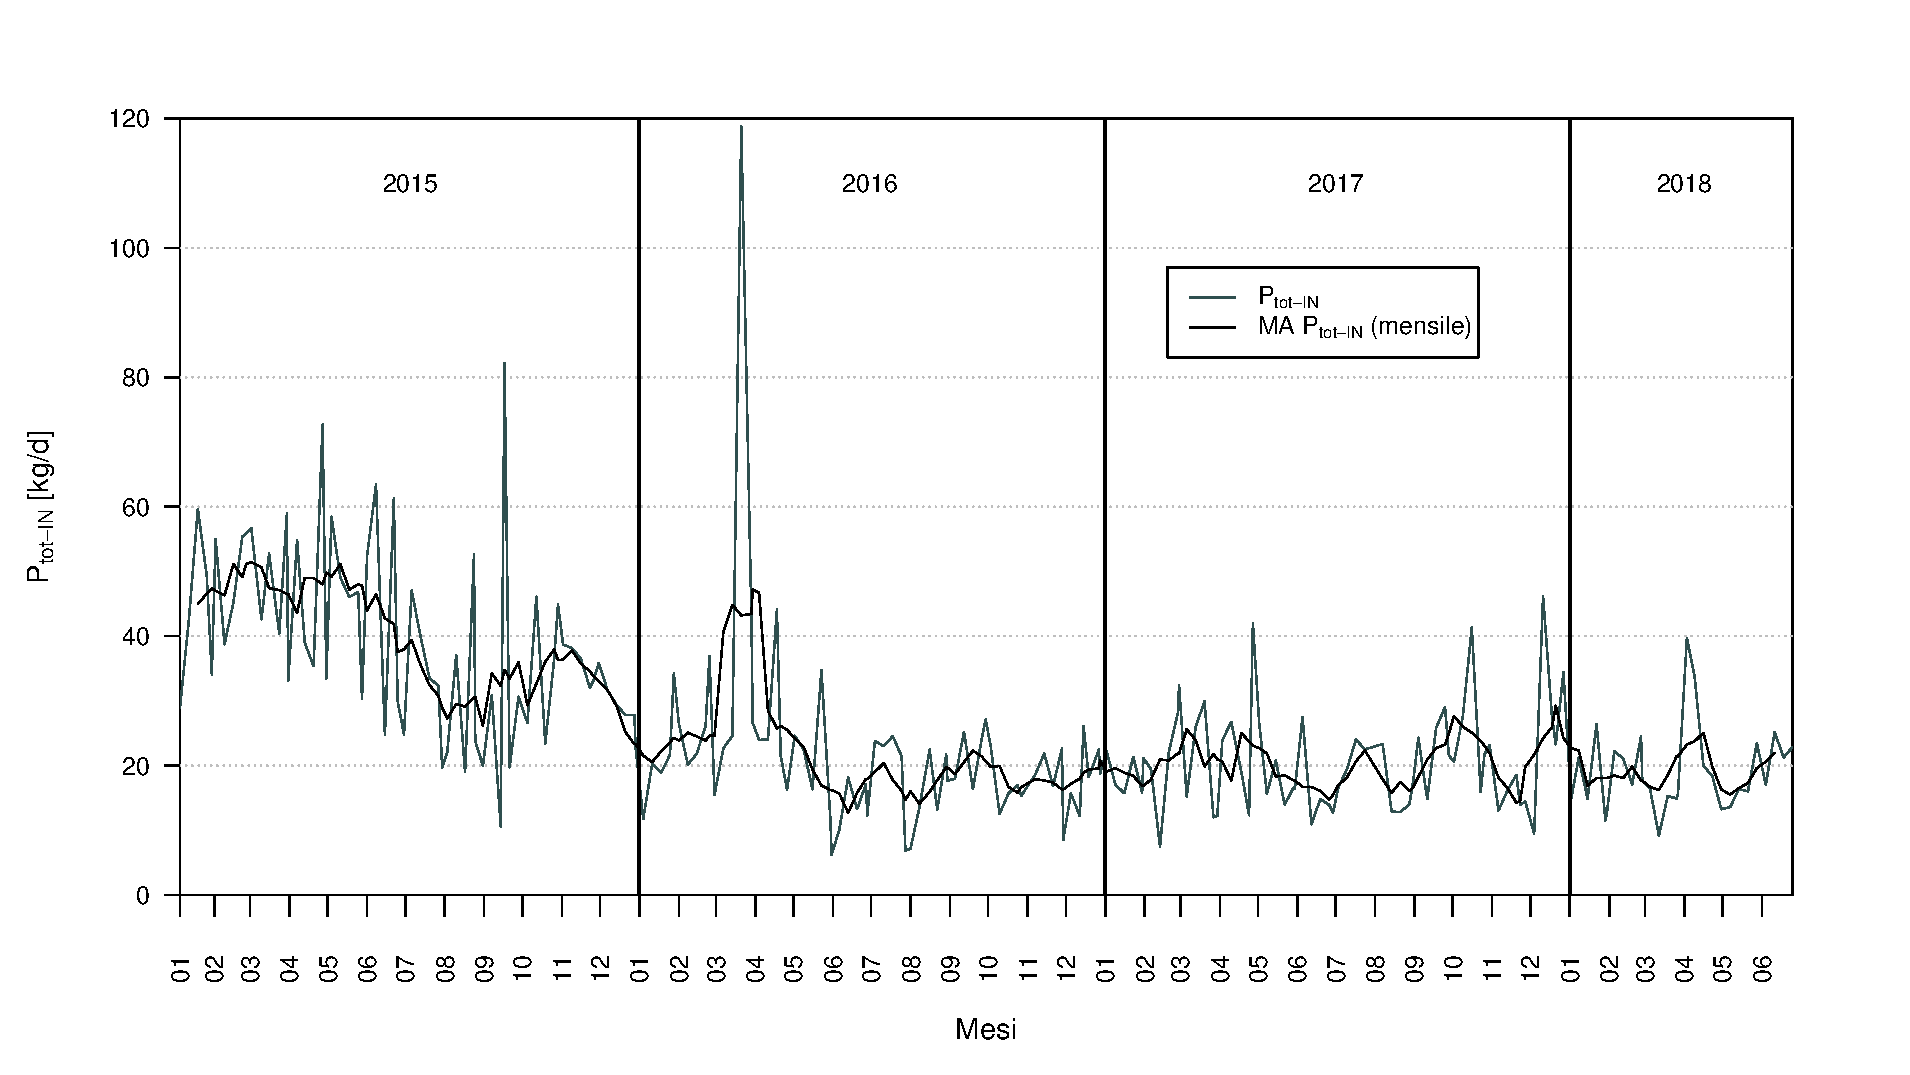
\includegraphics[width=\linewidth]{sa_car_Ptot}}
	\centering
	\caption{Andamento del carico in ingresso di fosforo totale}
	\label{fig:sa_car_Ptot}
\end{figure}
\begin{figure}[H]
	\fbox{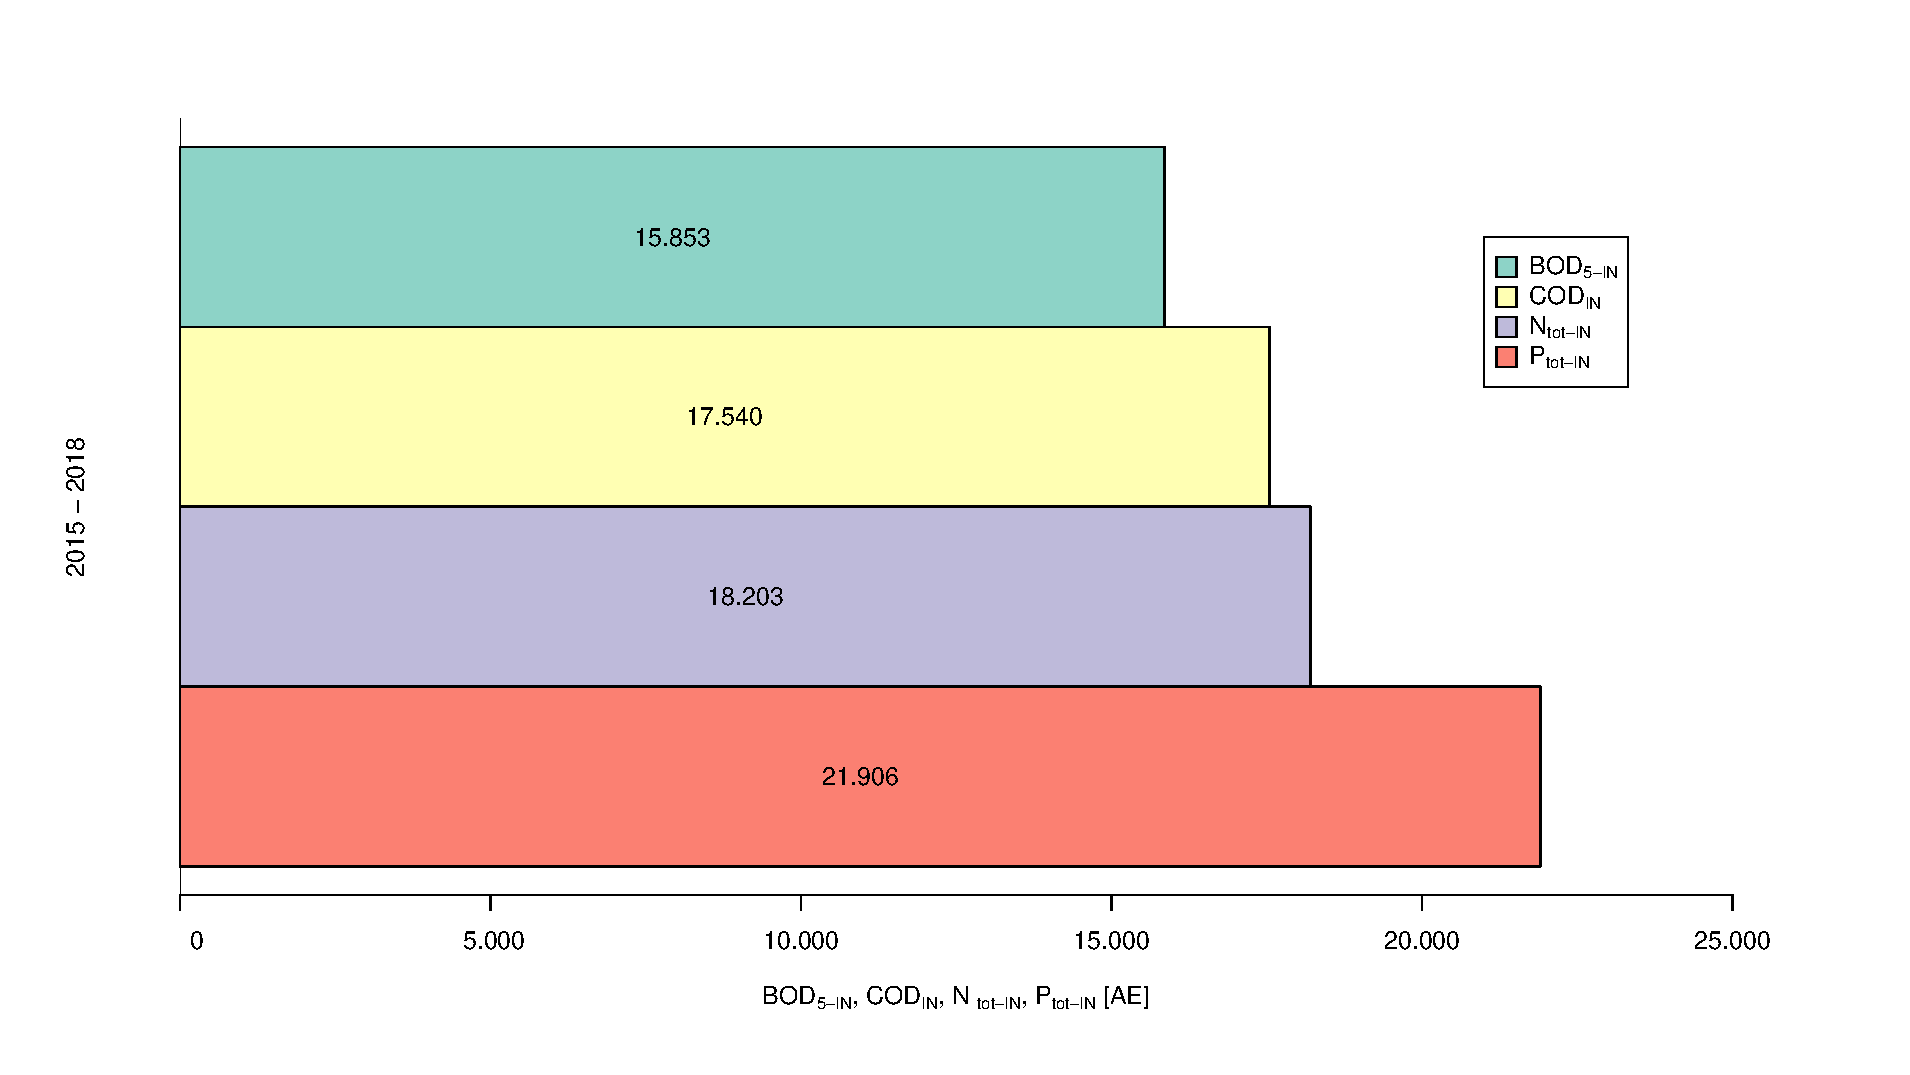
\includegraphics[width=\linewidth]{sa_AEtot}}
	\centering
	\caption{Carichi medi in ingresso di BOD\textsubscript{5} (60 g ab\textsuperscript{-1} d\textsuperscript{-1}), COD (120 g ab\textsuperscript{-1} d\textsuperscript{-1}), azoto totale (12 g ab\textsuperscript{-1} d\textsuperscript{-1}) e fosforo totale (1,2 g ab\textsuperscript{-1} d\textsuperscript{-1}), espressi in abitanti equivalenti, calcolati sull'intero periodo 2015 - 2018}
	\label{fig:sa_AEtot}
\end{figure}
\begin{figure}[H]
	\fbox{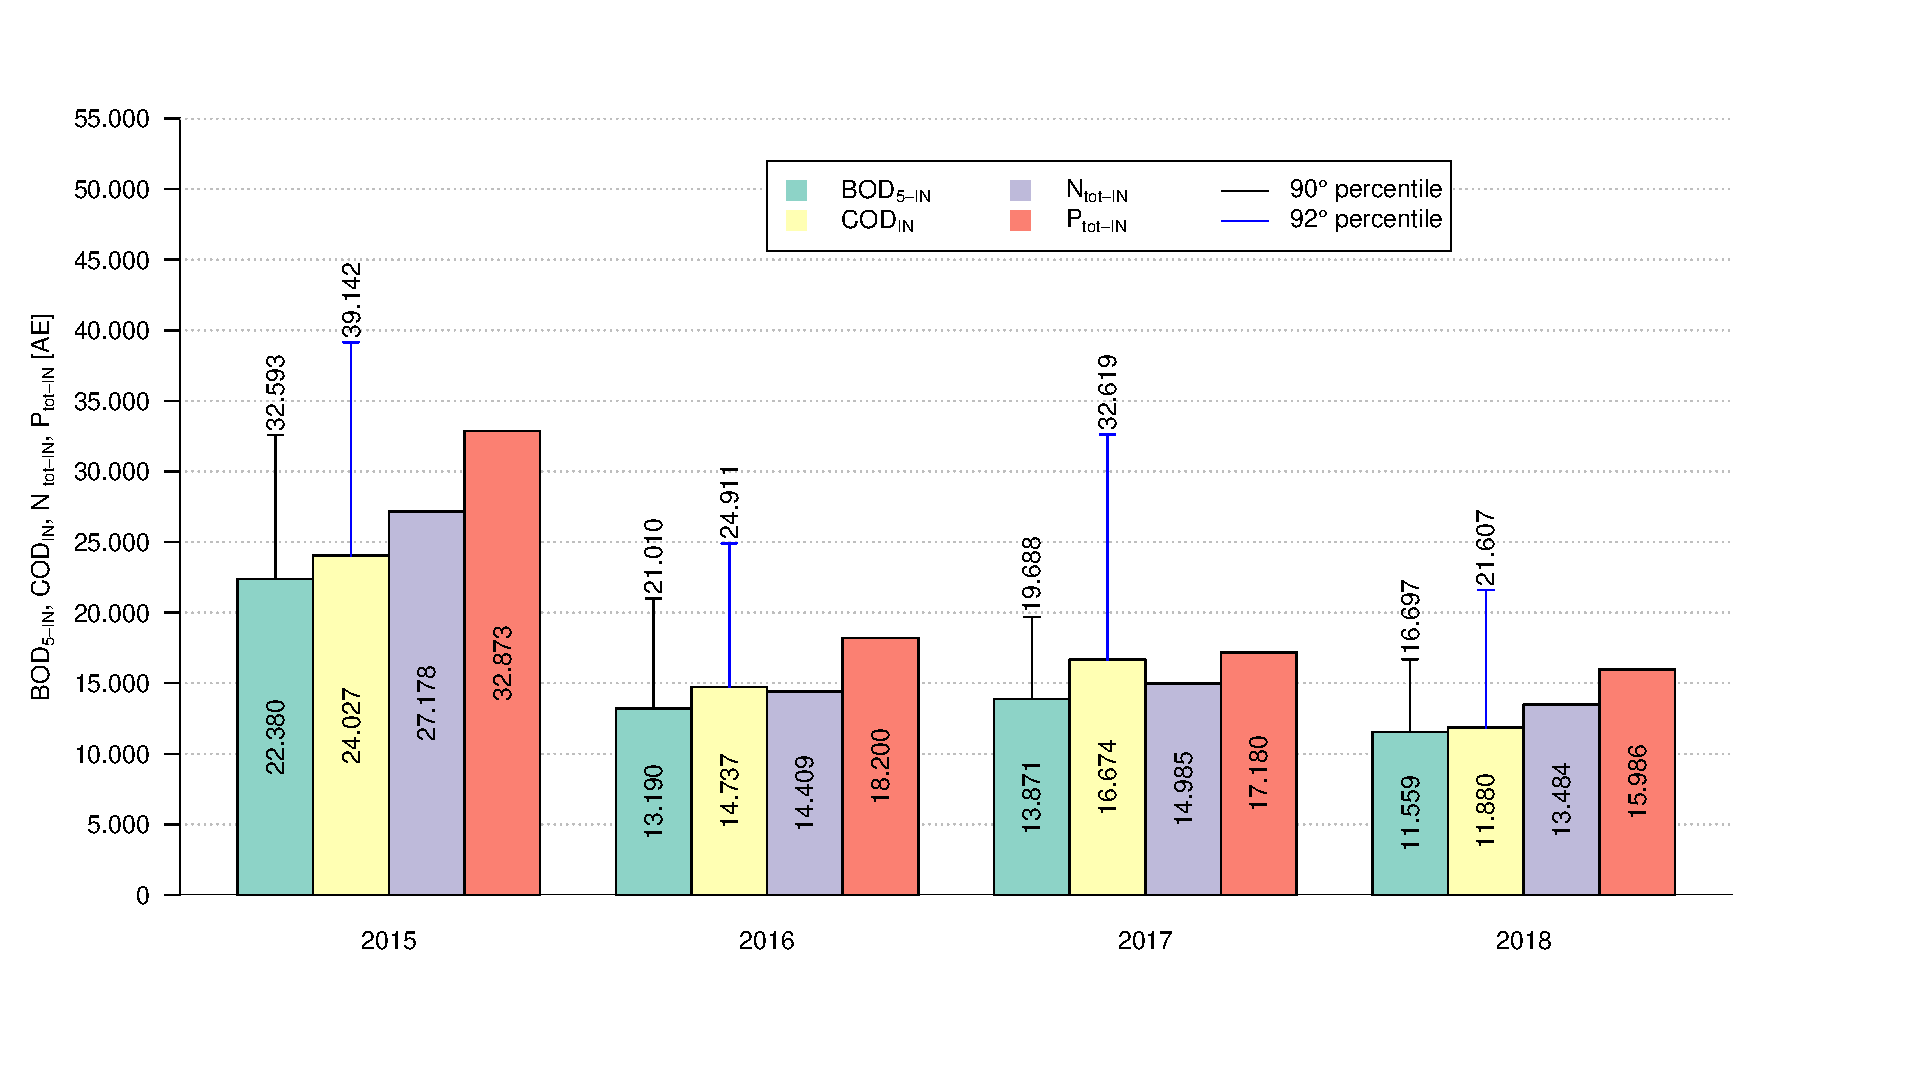
\includegraphics[width=\linewidth]{sa_AEanni}}	\centering
	\caption{Carichi medi annui in ingresso di BOD\textsubscript{5} (60 g ab\textsuperscript{-1} d\textsuperscript{-1}), COD (120 g ab\textsuperscript{-1} d\textsuperscript{-1}), azoto totale (12 g ab\textsuperscript{-1} d\textsuperscript{-1}) e fosforo totale (1,2 g ab\textsuperscript{-1} d\textsuperscript{-1}), espressi in abitanti equivalenti, calcolati per ciascun anno}
	\label{fig:sa_AEanni}
\end{figure}
Per l'intero periodo considerato e per ciascun anno, secondo quanto indicato nella \autoref{subsec:carichi}, sono stati calcolati i carichi medi annui di BOD\textsubscript{5}, COD, azoto totale e fosforo totale espressi in abitanti equivalenti (\autoref{fig:sa_AEtot} e \autoref{fig:sa_AEanni}). I carichi medi annui sono ben al di sotto della potenzialità di progetto (30.000 AE), che risulta anche quasi sempre compatibile con i valori del 90° percentile per il BOD\textsubscript{5} e del 92° percentile per il COD (non si considera l'anno 2015 perché la sua portata esibisce un comportamento anomalo). Si sono considerati proprio questi due percentili perché, in base a quanto spiegato nella \autoref{sec:limiti_scarico}, è consentito eccedere la potenzialità di progetto nel 10\% dei giorni per il BOD\textsubscript{5} e nell'8\% per il COD\footnote{Per l'anno 2018 si è stimato che, a fine anno, si avrà un numero di misurazioni doppio rispetto a quello conteggiato a fine giugno, assumendo che la media dei carichi sul primo semestre sia rappresentativa di quella annuale. Ovviamente questa analisi andrà ripetuta a fine anno, quando si sarà in possesso di tutti i dati.}.


\subsubsection{Caratteristiche dell'effluente}

I limiti di legge che devono essere rispettati dall'effluente sono stati indicati in \autoref{tab:sa_limiti}.

\paragraph{Caratteristiche qualitative}

\begin{figure}[H]
	\fbox{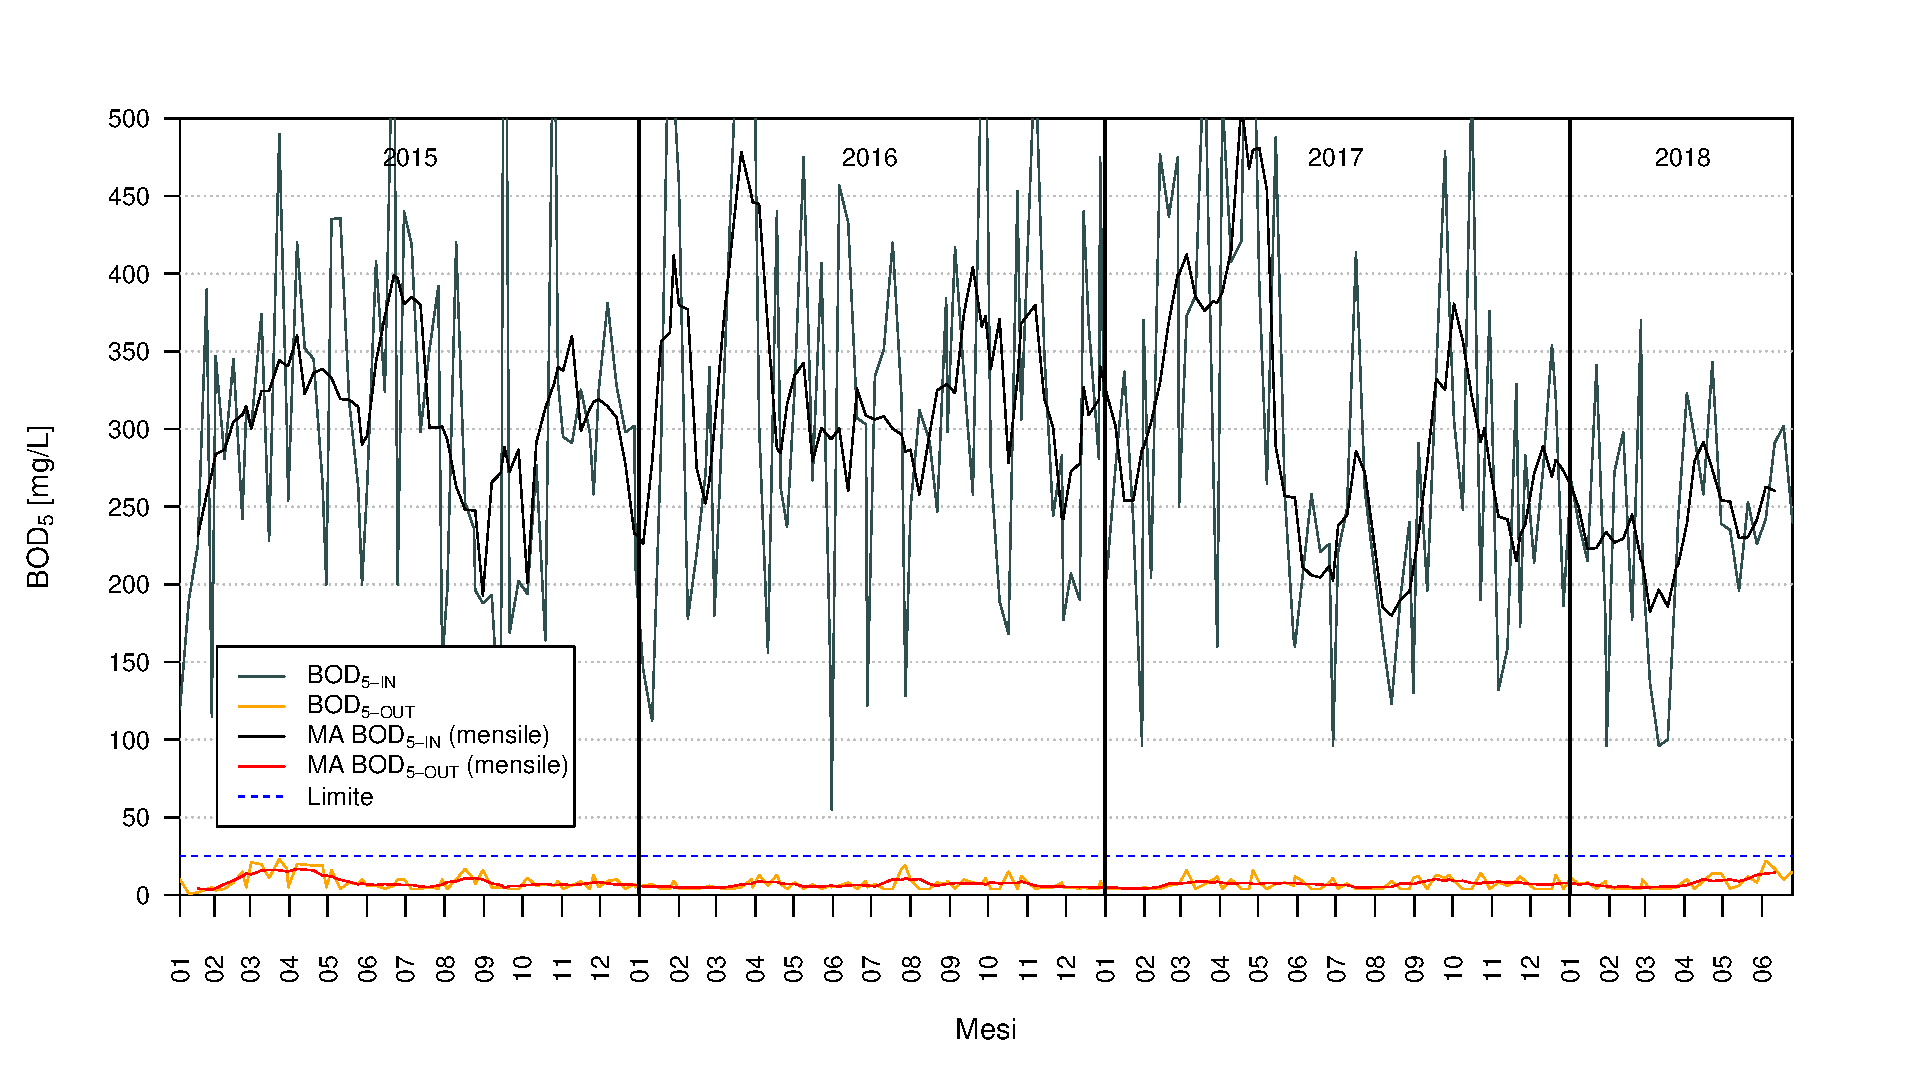
\includegraphics[width=\linewidth]{sa_BODout}}	\centering
	\caption{Andamento delle concentrazioni di BOD\textsubscript{5} in ingresso e in uscita}
	\label{fig:sa_BODout}
\end{figure}

La \autoref{fig:sa_BODout} rappresenta i valori di concentrazione di BOD\textsubscript{5} in ingresso e in uscita.
Per tutto l’arco temporale esaminato, la concentrazione di BOD\textsubscript{5} in uscita rispetta il limite di 25 mg/L con ampio margine. Essa è pressoché costante (attorno a un valore medio di 6,9 mg/L), ad eccezione di alcuni picchi che si mantengono comunque al di sotto del limite. \\

\begin{figure}[H]
	\fbox{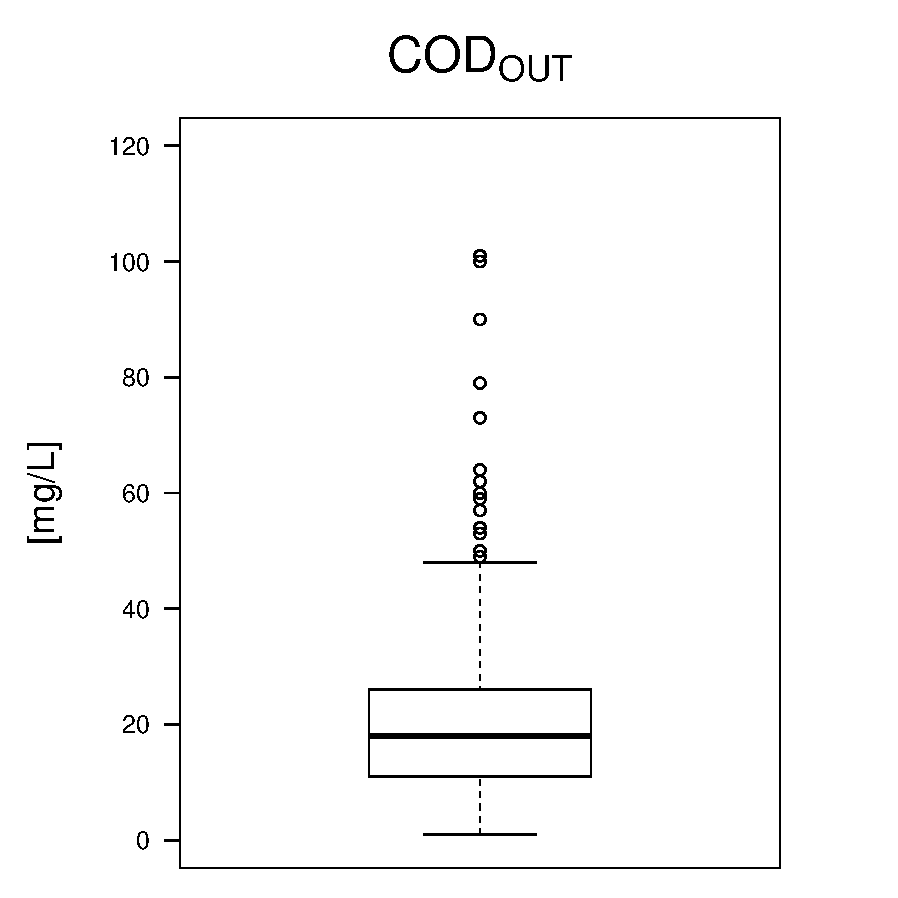
\includegraphics[width=\linewidth]{sa_CODout}}	\centering
	\caption{Andamento delle concentrazioni di COD in ingresso e in uscita}
	\label{fig:sa_CODout}
\end{figure}

I valori di COD in ingresso e in uscita, invece, sono rappresentati in \autoref{fig:sa_CODout}.
Per tutto il periodo esaminato, la concentrazione di COD in uscita rispetta il limite di 125 mg/L con ampio margine. Essa è pressoché costante (in media pari a 19,6 mg/L), soprattutto nel 2017 e nel 2018, nonostante ci sia un valore di COD in ingresso particolarmente elevato a fine 2017. Di conseguenza non si ha correlazione tra concentrazione in ingresso e concentrazione in uscita.

Durante l’intero arco temporale considerato, la concentrazione di SST in uscita rispetta il limite di 35 mg/L con ampio margine, ad eccezione di alcuni picchi che si mantengono comunque al di sotto del limite. Tale concentrazione è pressoché costante, in media circa 7,7 mg/L (\autoref{fig:sa_SSTout-1q}).
\begin{figure}[H]
	\fbox{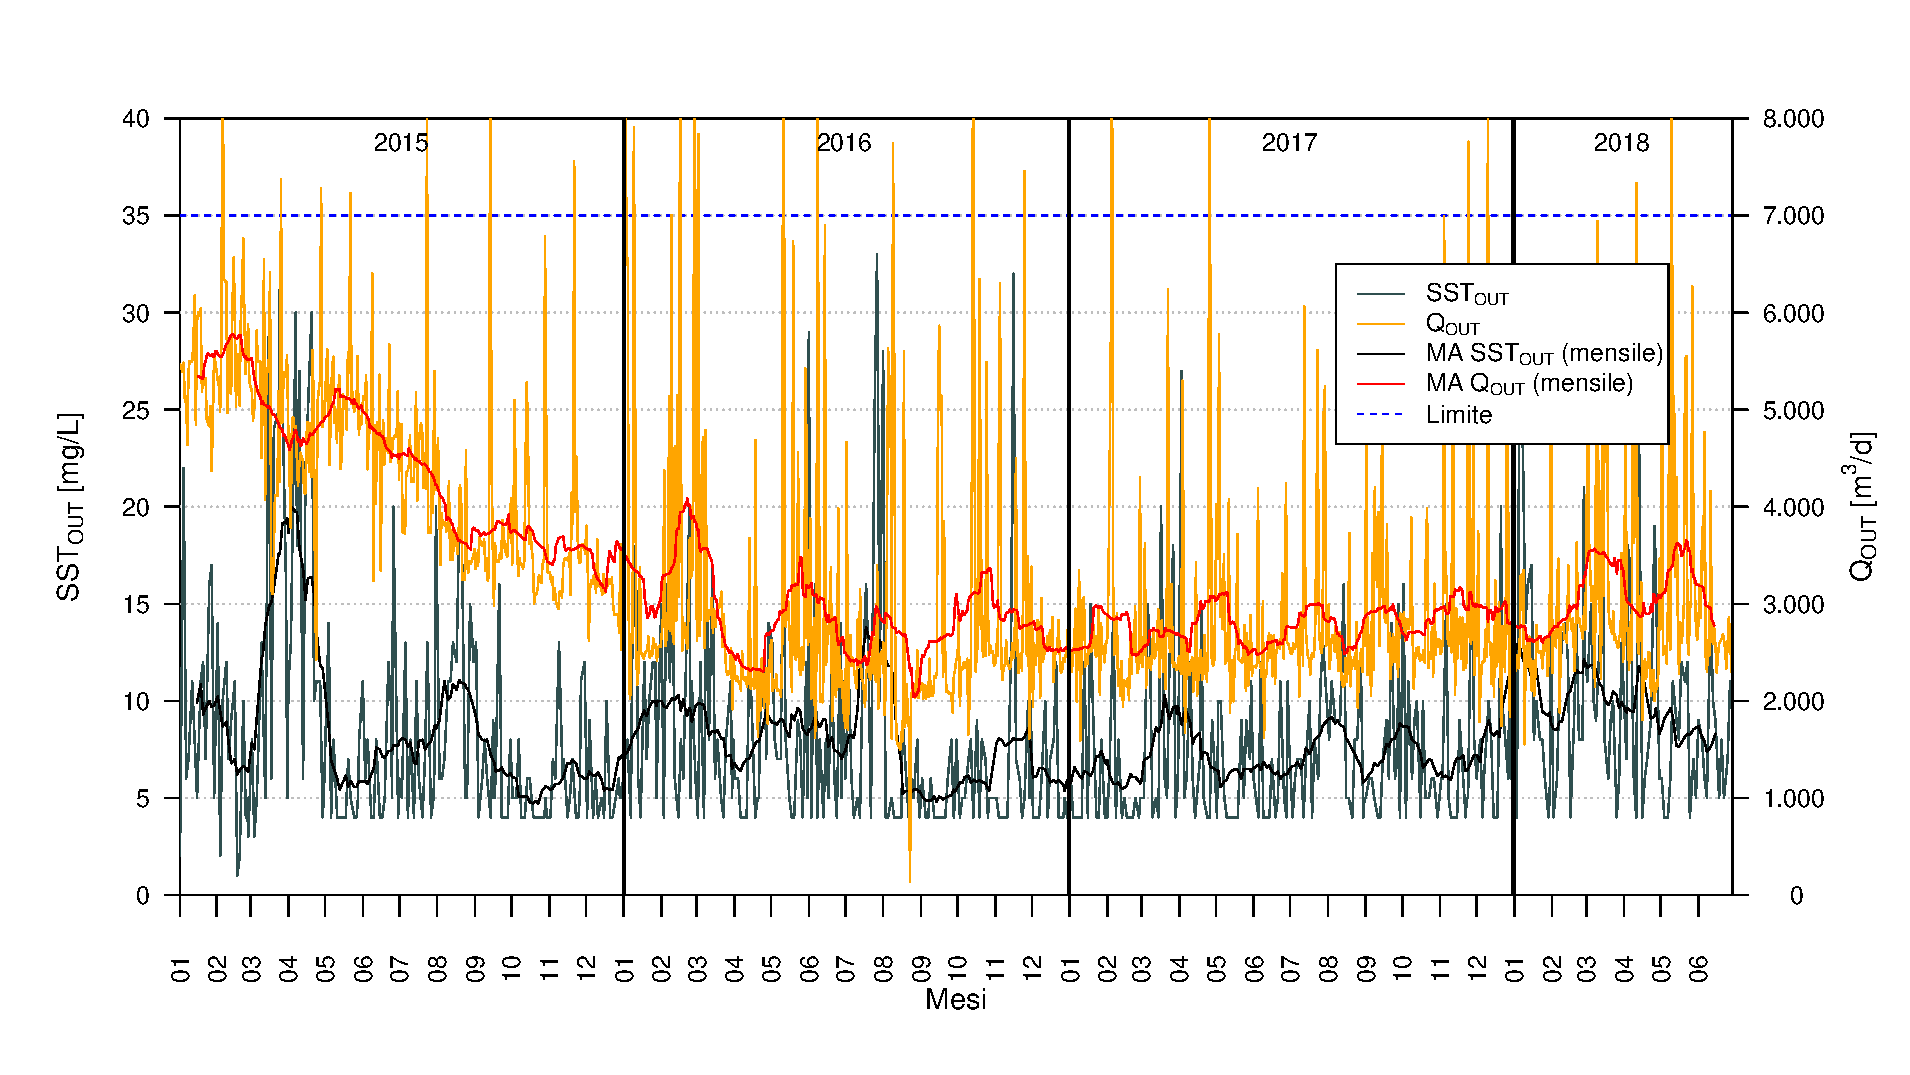
\includegraphics[width=\linewidth]{sa_SSTout-1q}}	\centering
	\caption{Andamento della concentrazione in uscita di SST e della portata effluente}
	\label{fig:sa_SSTout-1q}
\end{figure}
L'andamento della concentrazione in uscita di SST può essere confrontato con la portata effluente al fine di valutare l'efficienza della sedimentazione finale.
In alcuni intervalli temporali si riesce ad associare un incremento di concentrazione di SST a un aumento di portata. In ogni caso, la concentrazione di SST in uscita è sempre notevolmente inferiore al limite di legge e quindi l'eventuale effetto di trascinamento dei solidi sospesi, dovuto all'aumento della portata, non compromette la qualità dell'effluente.

Nel grafico di \autoref{fig:sa_Ntotout} sono rappresentate le concentrazioni in ingresso e in uscita di azoto totale.
Da questa rappresentazione si ricava un’idea generale dell’efficacia di rimozione complessiva dell’azoto che si può ritenere soddisfacente.
\begin{figure}[H]
	\fbox{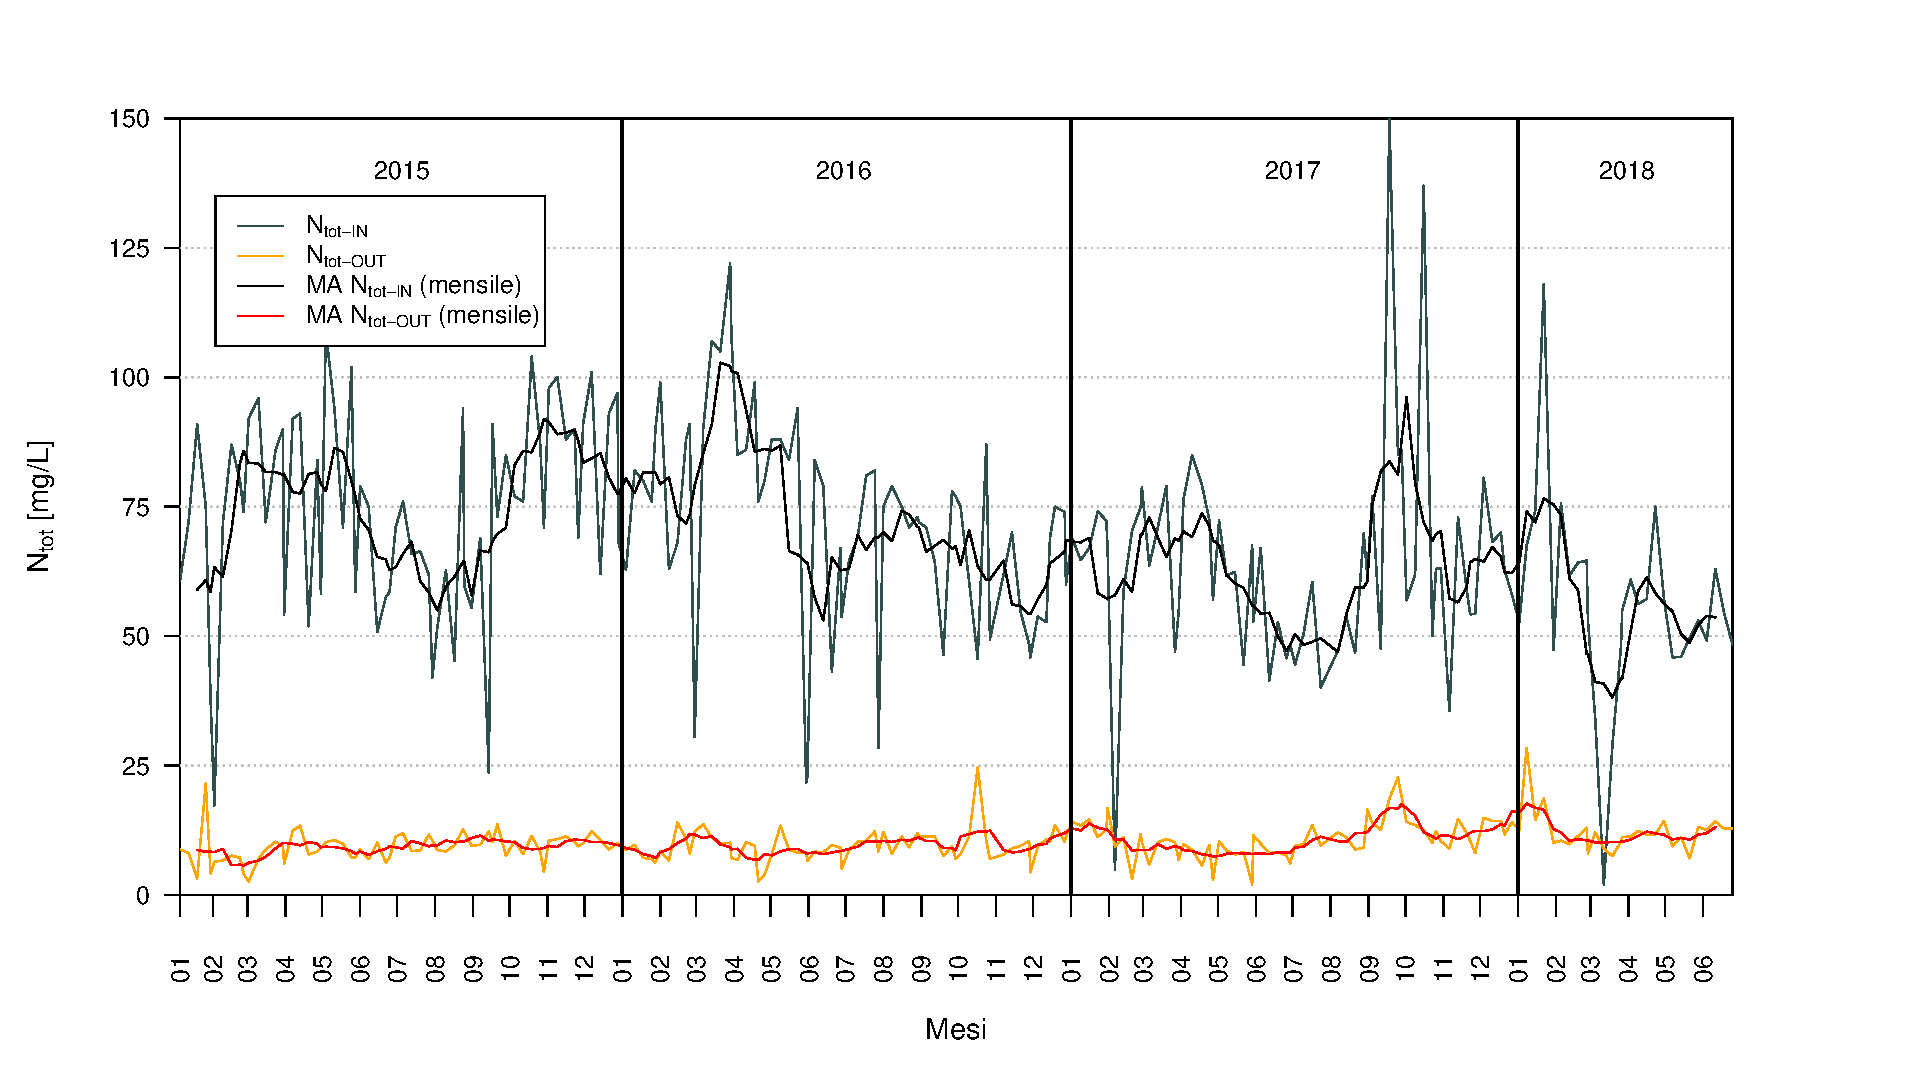
\includegraphics[width=\linewidth]{sa_Ntotout}}	\centering
	\caption{Andamento delle concentrazioni di azoto totale in ingresso e in uscita}
	\label{fig:sa_Ntotout}
\end{figure}
\begin{figure}[H]
	\fbox{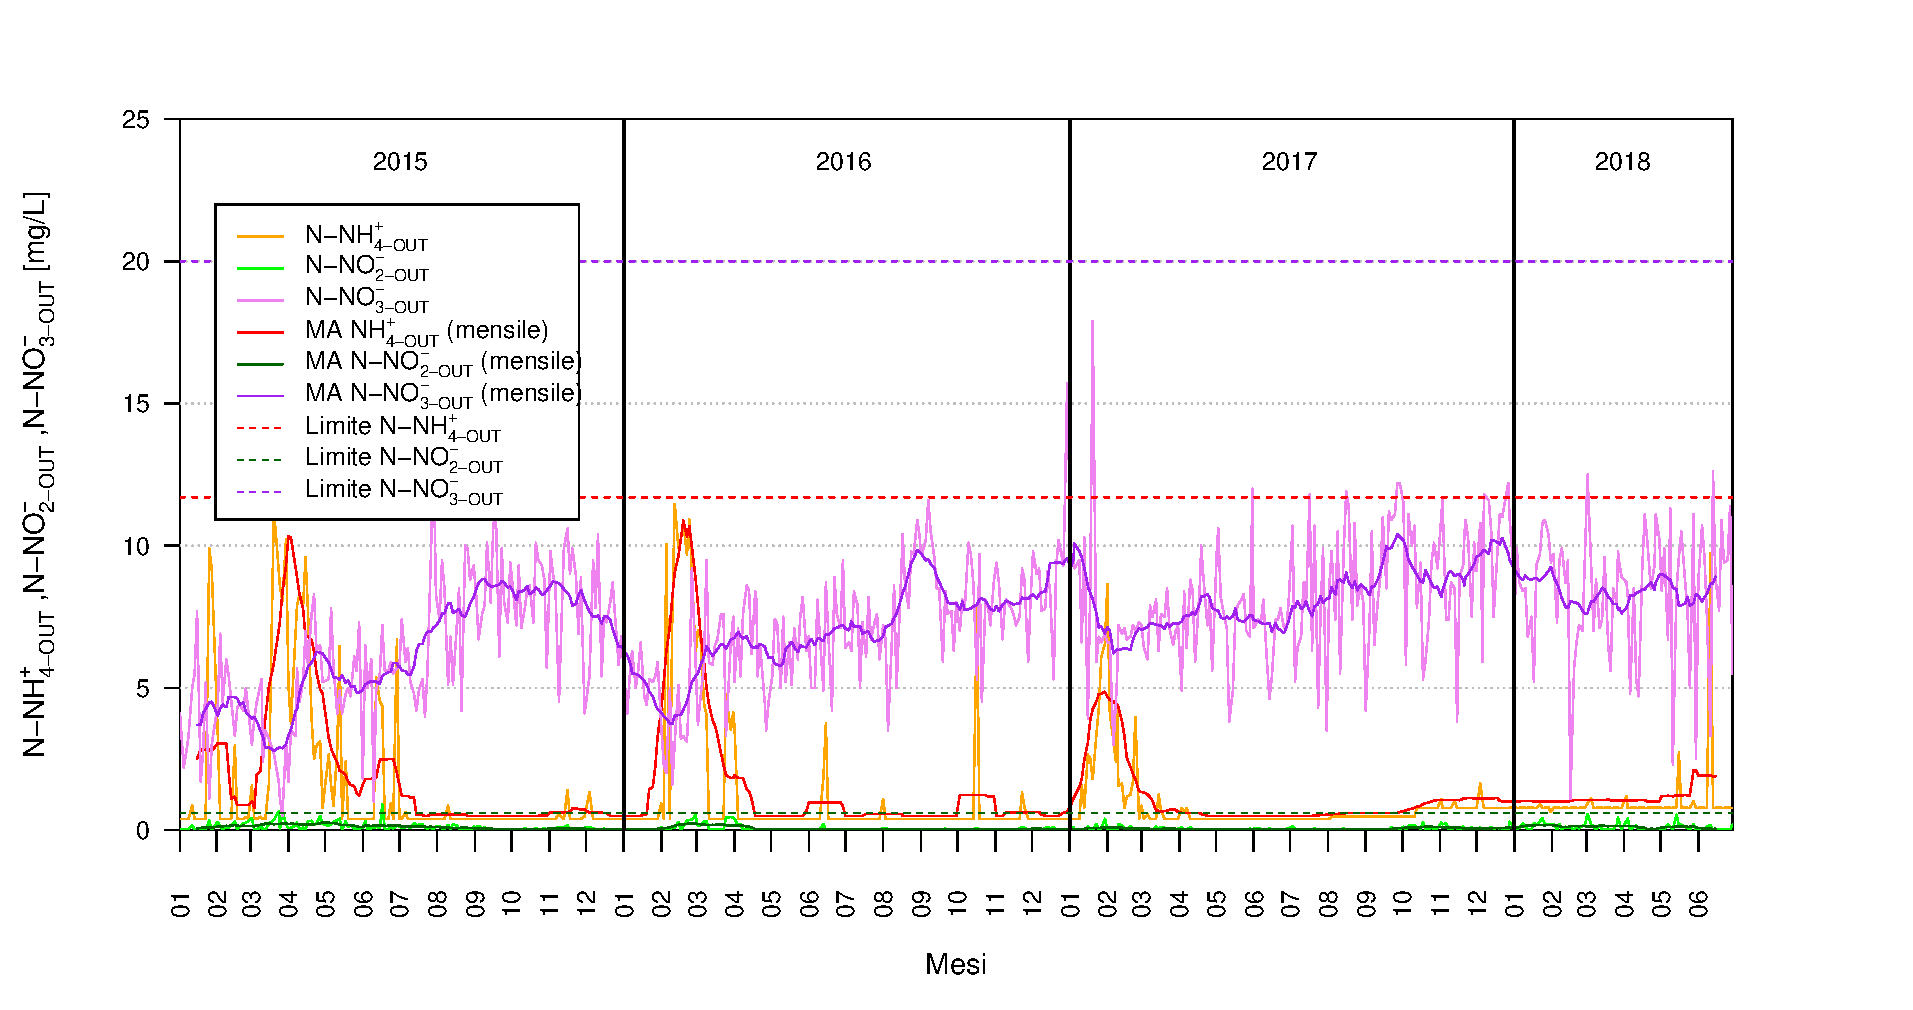
\includegraphics[width=\linewidth]{sa_NH4-NO2-NO3out}}	\centering
	\caption{Andamento delle concentrazioni in uscita di azoto ammoniacale, azoto nitroso e azoto nitrico}
	\label{fig:sa_NH4-NO2-NO3out}
\end{figure}

Le concentrazioni in uscita di azoto ammoniacale (N-NH\textsubscript{4}\textsuperscript{+}), azoto nitroso (N-NO\textsubscript{2}\textsuperscript{-}) e azoto nitrico (N-NO\textsubscript{3}\textsuperscript{-}), durante il periodo considerato, si mantengono al di sotto del proprio limite allo scarico (\autoref{fig:sa_NH4-NO2-NO3out}).
Si nota che, in corrispondenza dei picchi di N-NH\textsubscript{4}\textsuperscript{+}, si hanno anche picchi di N-NO\textsubscript{2}\textsuperscript{-}. Molto evidente è il drastico calo del rendimento di nitrificazione in alcuni periodi con bassa temperatura (si vedano i picchi di marzo-aprile 2015, febbraio 2016, febbraio 2017 e giugno 2018).
\begin{figure}[H]
	\fbox{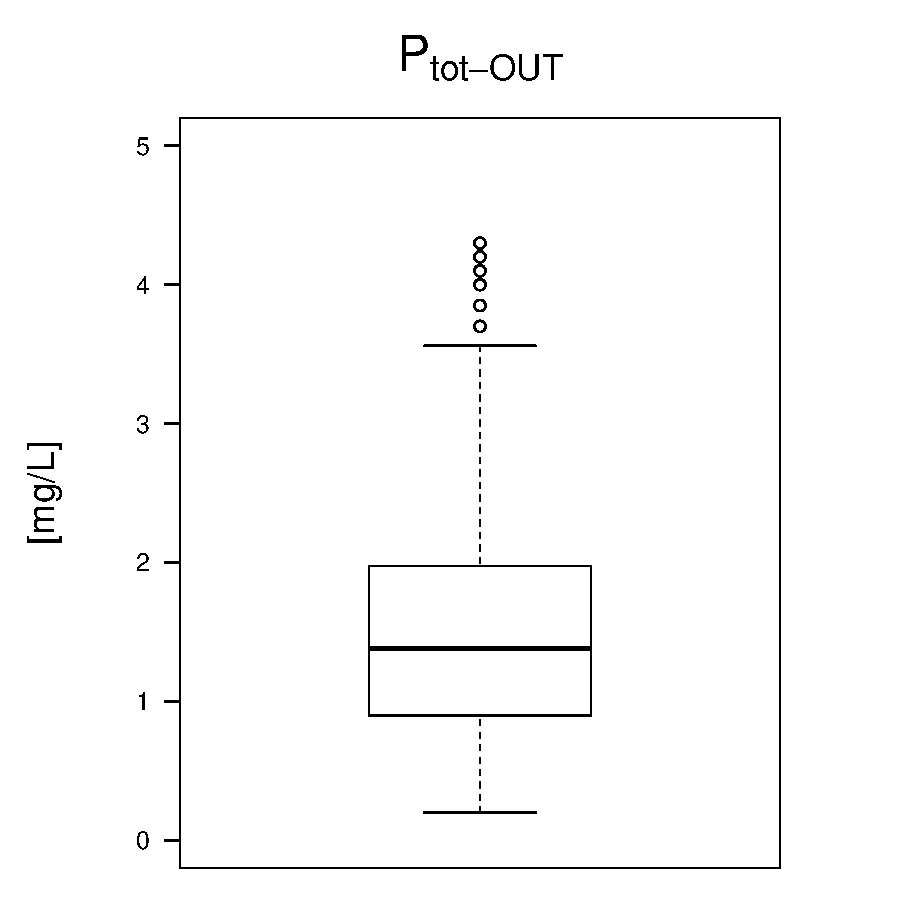
\includegraphics[width=\linewidth]{sa_Ptotout}}	\centering
	\caption{Andamento delle concentrazioni di fosforo totale in ingresso e in uscita}
	\label{fig:sa_Ptotout}
\end{figure}

Nel grafico di \autoref{fig:sa_Ptotout} sono rappresentate le concentrazioni di fosforo totale in ingresso e in uscita.
Spesso la concentrazione di fosforo totale in ingresso è inferiore al limite allo scarico (10 mg/L) e, per l’intero arco temporale esaminato, la concentrazione in uscita rispetta tale limite con ampio margine.

Relativamente alla concentrazione in uscita di \textit{Escherichia coli}, ad eccezione di pochi casi isolati, il limite di 5.000 UFC/100 mL, imposto per i periodi compresi tra aprile e settembre, è rispettato (\autoref{fig:sa_ECout}).
\begin{figure}[H]
	\fbox{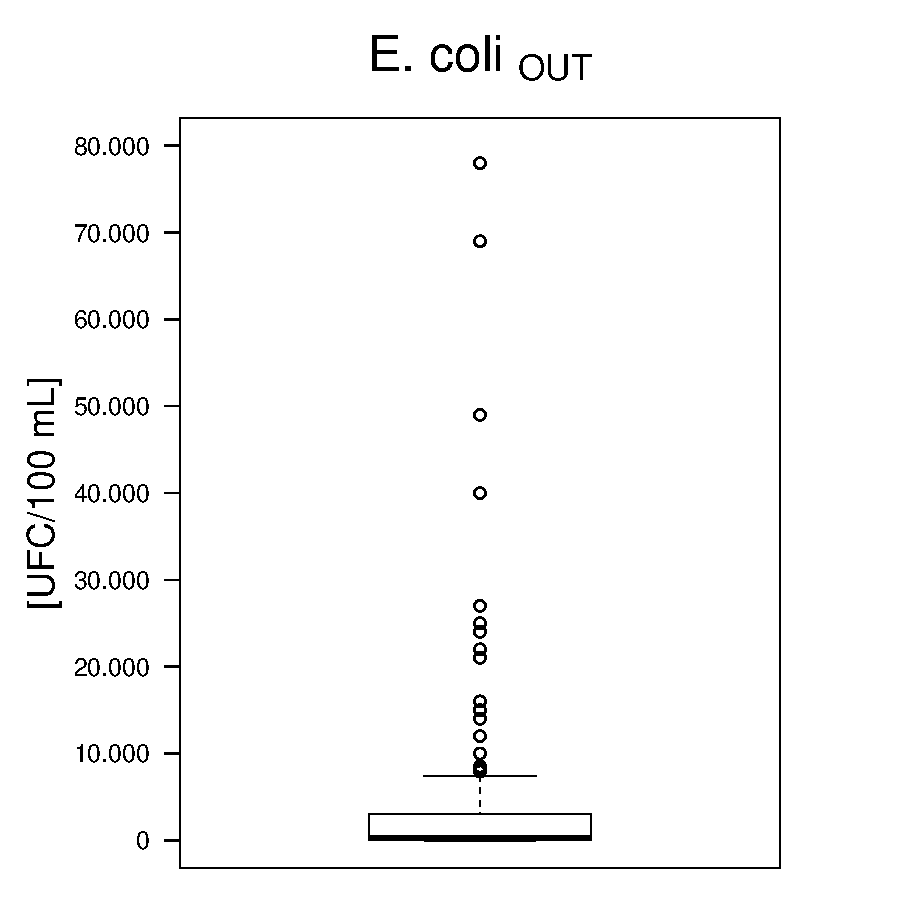
\includegraphics[width=\linewidth]{sa_ECout}}	\centering
	\caption{Andamento della concentrazione in uscita di \textit{Escherichia coli}}
	\label{fig:sa_ECout}
\end{figure}
\begin{figure}[H]
	\fbox{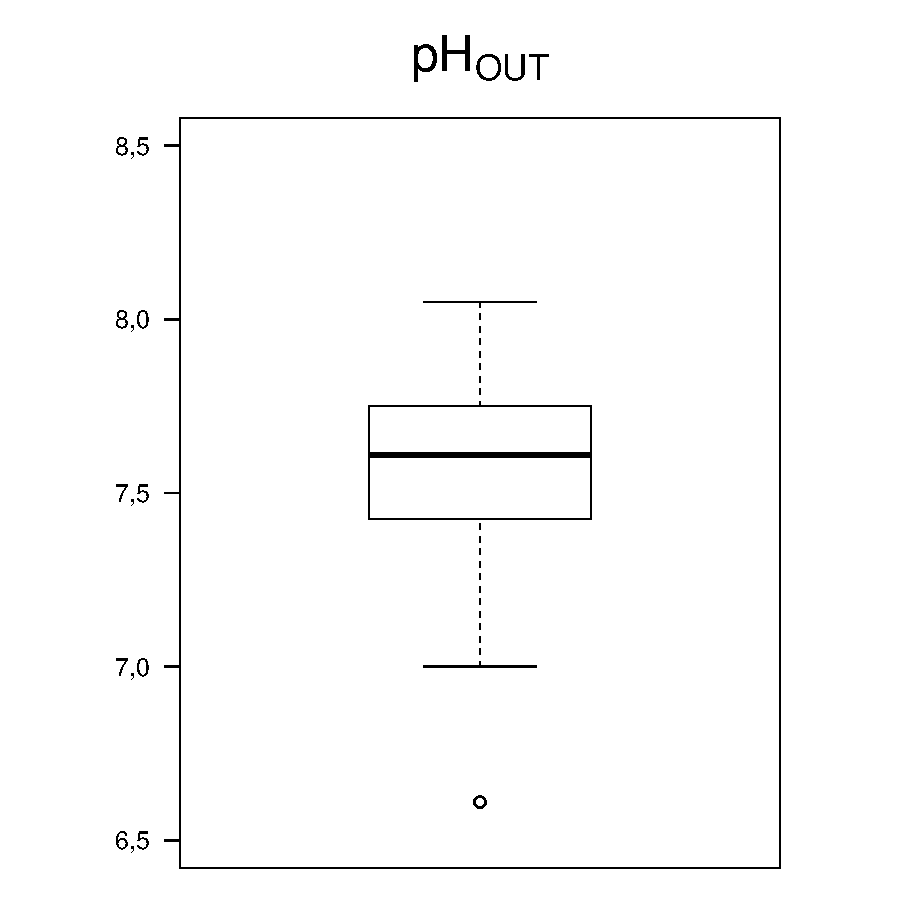
\includegraphics[width=\linewidth]{sa_pHout}}	\centering
	\caption{Andamento del pH del liquame in ingresso e in uscita}
	\label{fig:sa_pHout}
\end{figure}

Successivamente si sono confrontati i valori di pH in ingresso e in uscita (\autoref{fig:sa_pHout}).
Si nota che il pH in uscita è quasi sempre leggermente inferiore rispetto a quello in entrata. Esso tendenzialmente segue l’andamento dell’ingresso tranne a marzo 2017, da ottobre 2017 a febbraio 2018 (si ricorda che attorno al mese di ottobre 2017 si era individuato un picco di COD che dipende da un probabile ingresso di un refluo di origine industriale) e tra aprile e maggio 2018.

La temperatura in uscita, invece, è praticamente invariata rispetto a quella in ingresso (\autoref{fig:sa_Tout}).

\begin{figure}[H]
	\fbox{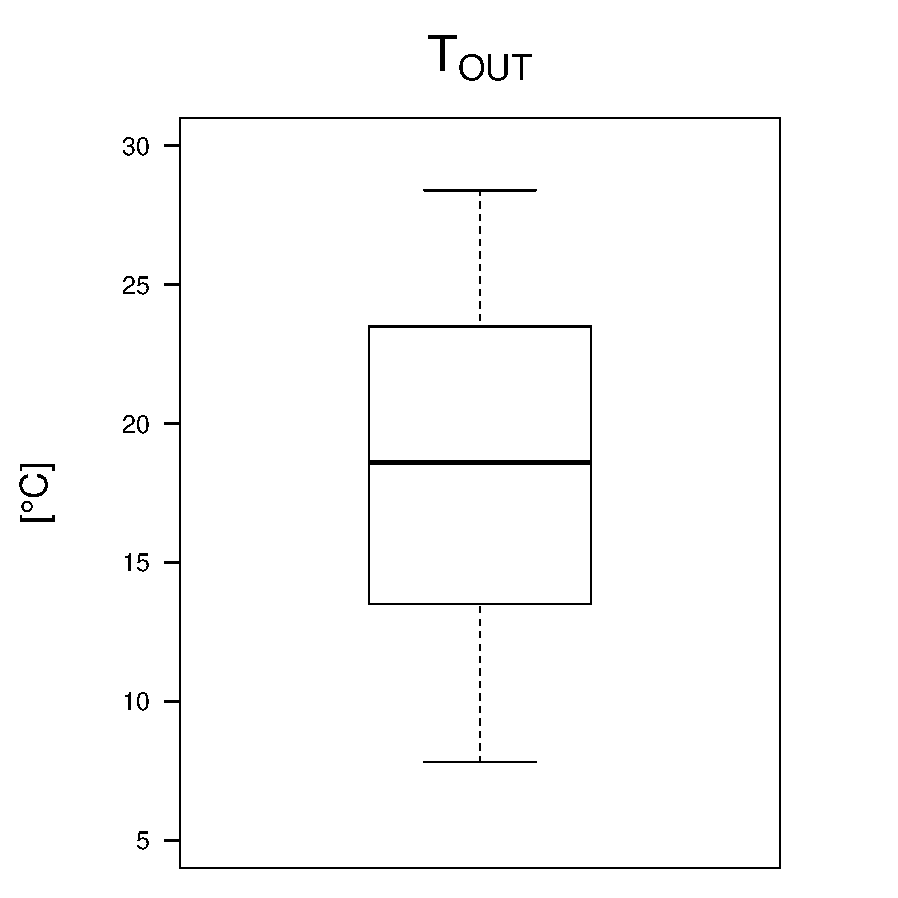
\includegraphics[width=\linewidth]{sa_Tout}}	\centering
	\caption{Andamento della temperatura del liquame in ingresso e in uscita}
	\label{fig:sa_Tout}
\end{figure}

\subsubsection{Prestazioni}
I rendimenti di rimozione dei carichi inquinanti sono stati calcolati come spiegato nella \autoref{sec:rend}.
Essi sono stati determinati per ciascun anno (\autoref{fig:sa_rendanni}) e per il periodo complessivo in esame (\autoref{fig:sa_rendtot}).

Al passare del tempo, i rendimenti di rimozione di BOD\textsubscript{5} e COD rimangono stabili e superiori al 95\%. Nel caso dell'azoto, invece, la percentuale è in continua diminuzione. Il fosforo presenta un andamento simile ad esclusione dell'anno 2018, in cui si registra un miglioramento del rendimento che però non torna ad essere quello del 2015.
L'efficacia dei processi di nitrificazione non manifesta grandi variazioni, ma si è già evidenziato che si presentano, occasionalmente, importanti episodi di mancata nitrificazione. Il rendimento dei processi di denitrificazione, invece, peggiora nel tempo.
\begin{figure}[H]
	\fbox{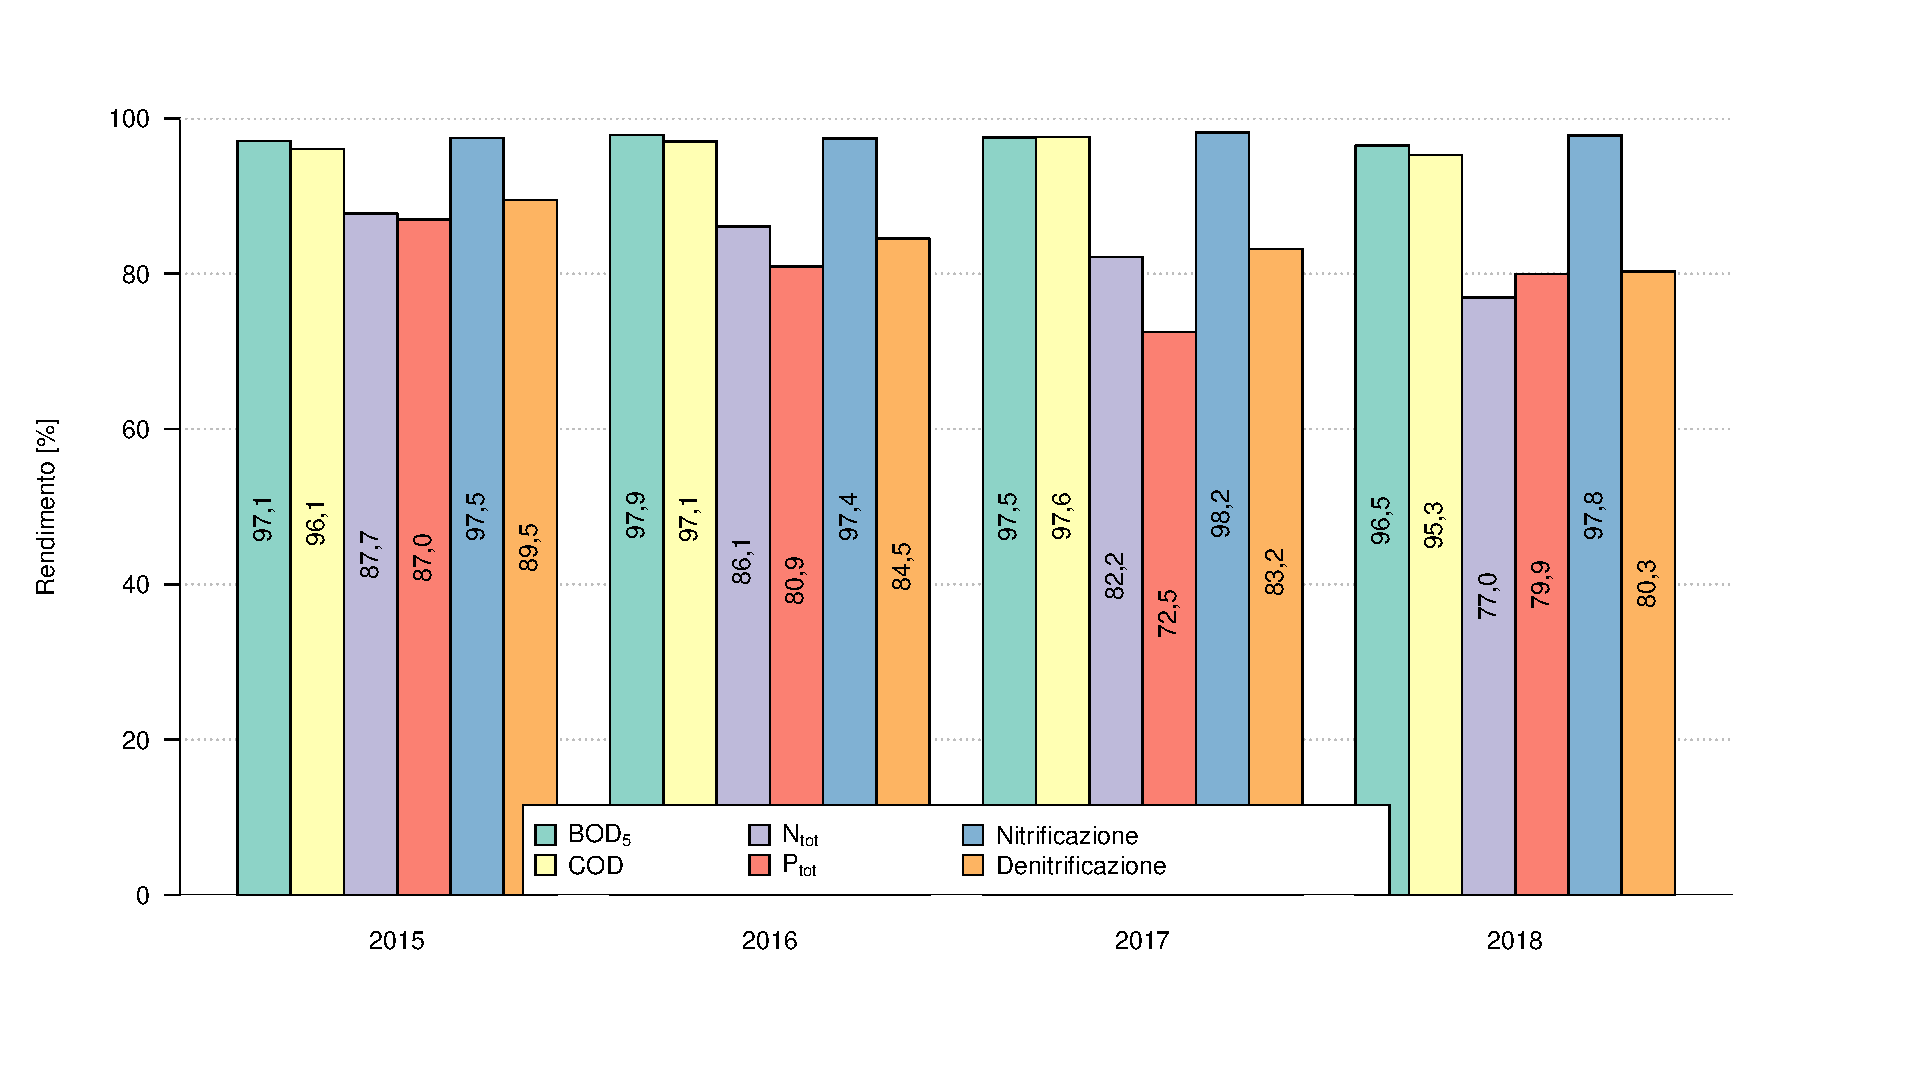
\includegraphics[width=\linewidth]{sa_rendanni}}	\centering
	\caption{Rendimenti di rimozione su base annua}
	\label{fig:sa_rendanni}
\end{figure}
\begin{figure}[H]
	\fbox{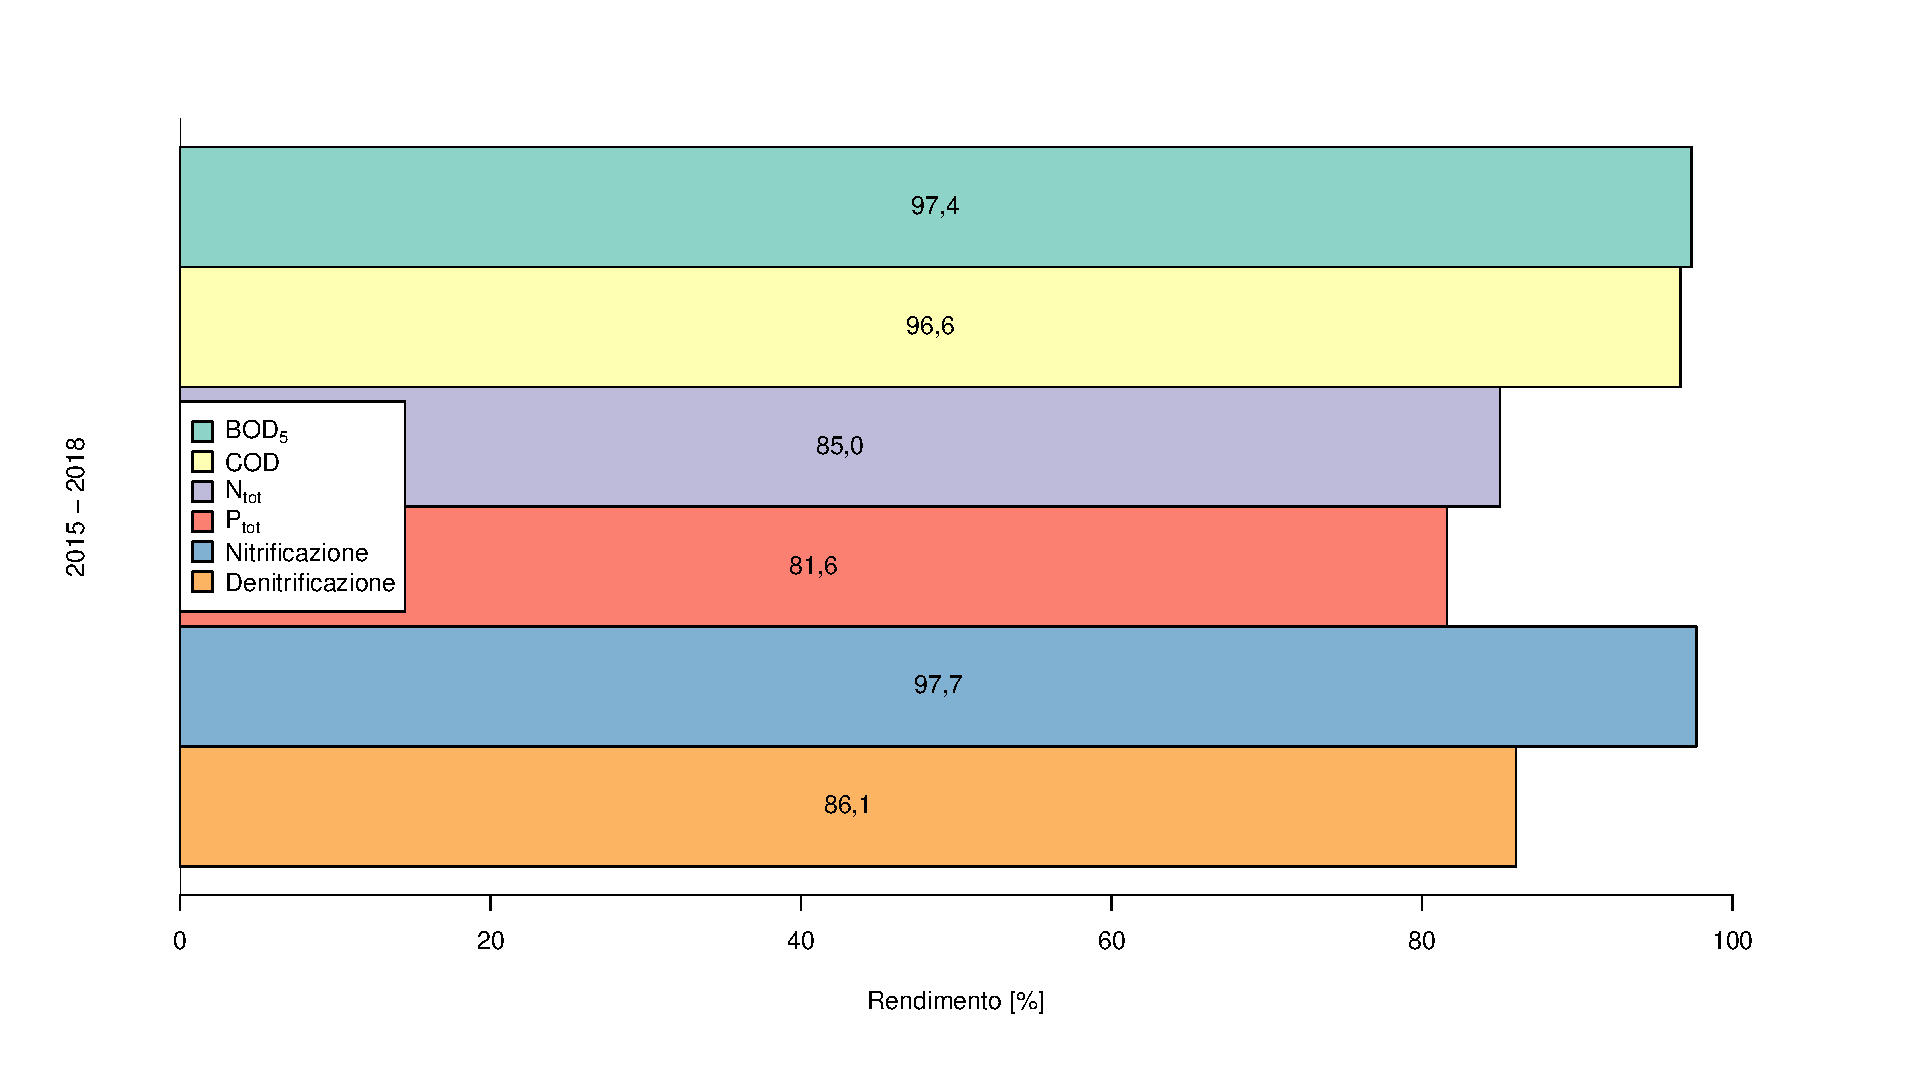
\includegraphics[width=\linewidth]{sa_rendtot}}	\centering
	\caption{Rendimenti di rimozione complessivi per il periodo 2015 - 2018}
	\label{fig:sa_rendtot}
\end{figure}

\subsubsection{Parametri operativi}

La variabilità di concentrazione di SST nelle vasche di ossidazione è principalmente compresa tra 2 e 6 g/L, come mostrato in \autoref{fig:sa_SSTox}. Le linee 1 e 2 sono caratterizzate da valori simili, mentre la linea 3 è maggiormente concentrata. Fatta eccezione per un periodo a cavallo degli anni 2017 e 2018, gli aumenti e le diminuzioni di concentrazione sono contemporanei in tutte le linee. Non sembra esserci, invece, correlazione con il carico in ingresso di COD. Si può scorgere inoltre, soprattutto per le linee 1 e 2, una periodicità.

\begin{figure}[H]
	\fbox{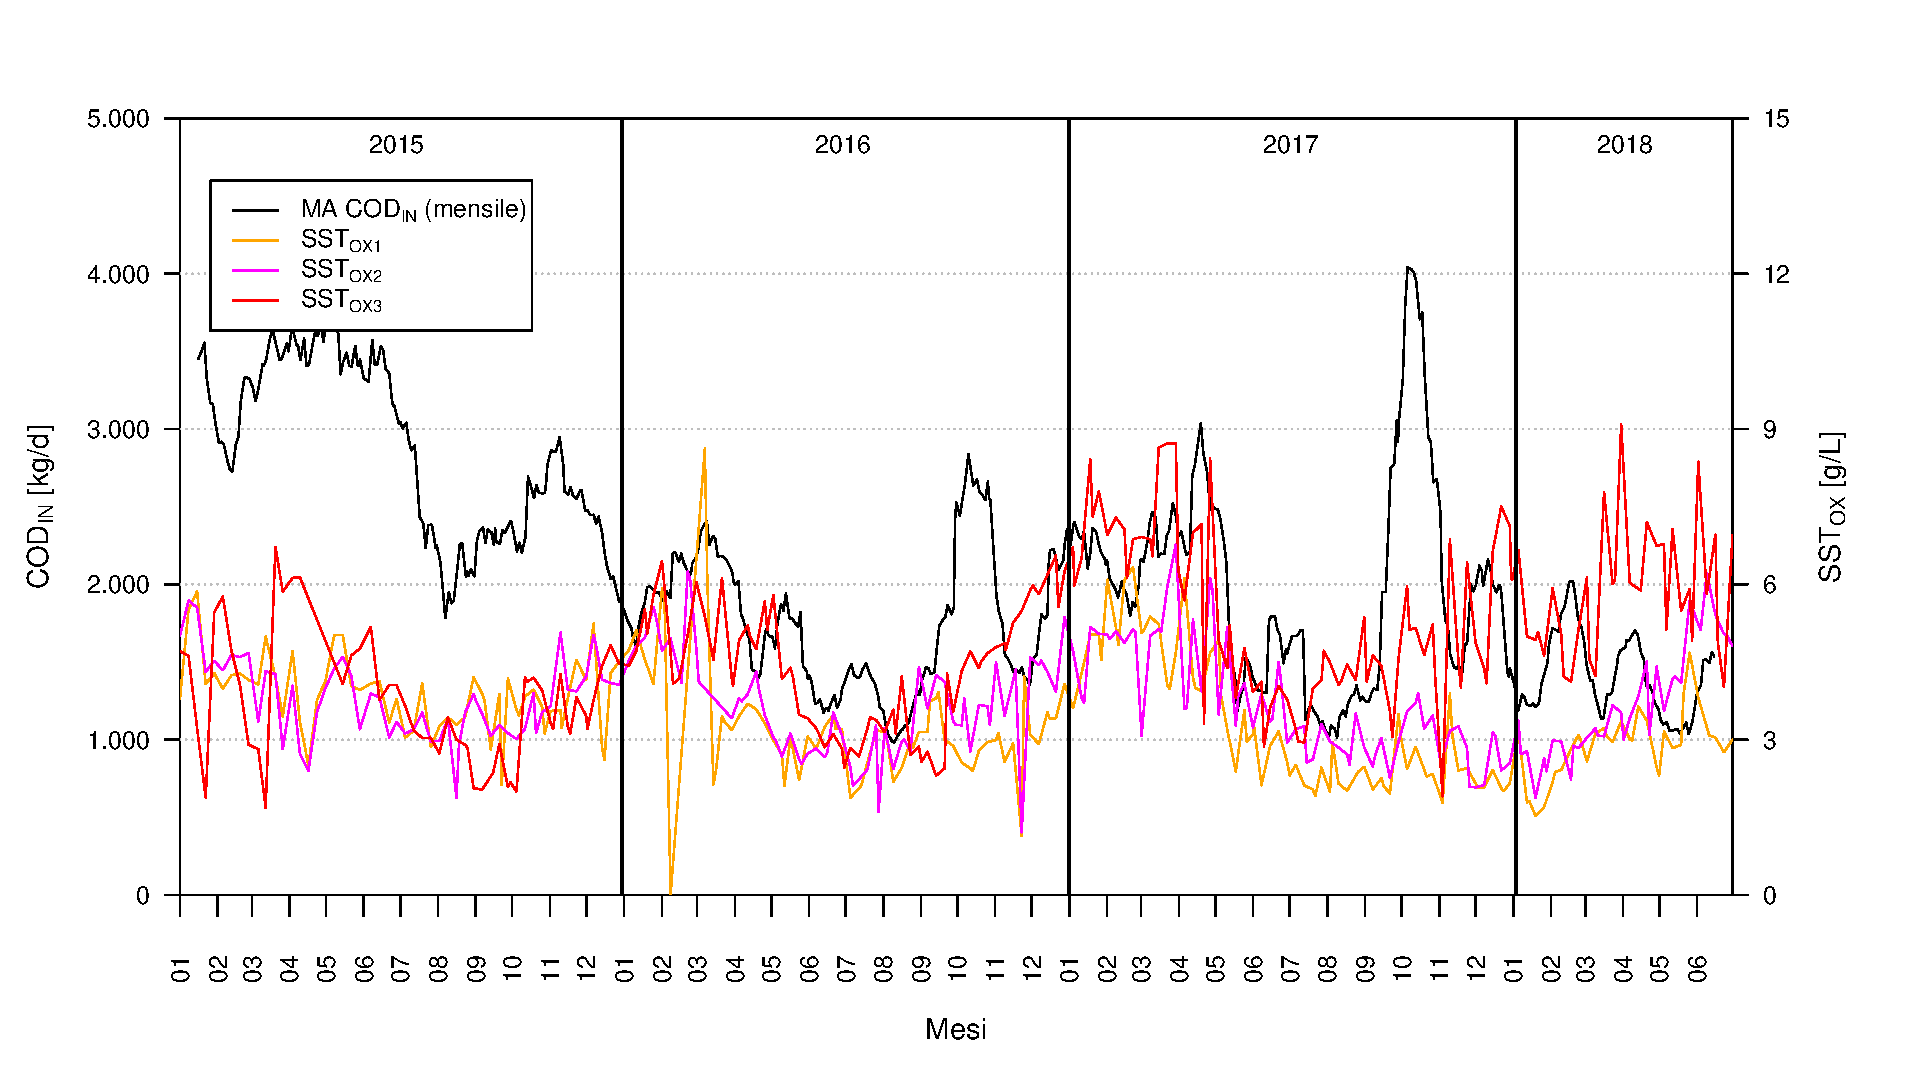
\includegraphics[width=\linewidth]{sa_SSTox}}	\centering
	\caption{Andamento della concentrazione di SST nelle vasche di ossidazione e del carico in ingresso di COD}
	\label{fig:sa_SSTox}
\end{figure}

Anche nel caso del fango di ricircolo la concentrazione di SST è piuttosto oscillante (\autoref{fig:sa_SSTric}). I tre andamenti sono perlopiù correlati e sono compresi tra 2 e 8 g/L. Se si confrontano tali valori con quelli  delle vasche di ossidazione, si osserva che sono abbastanza bassi (generalmente le concentrazioni nel ricircolo sono circa il doppio di quelle nel comparto biologico).

\begin{figure}[H]
	\fbox{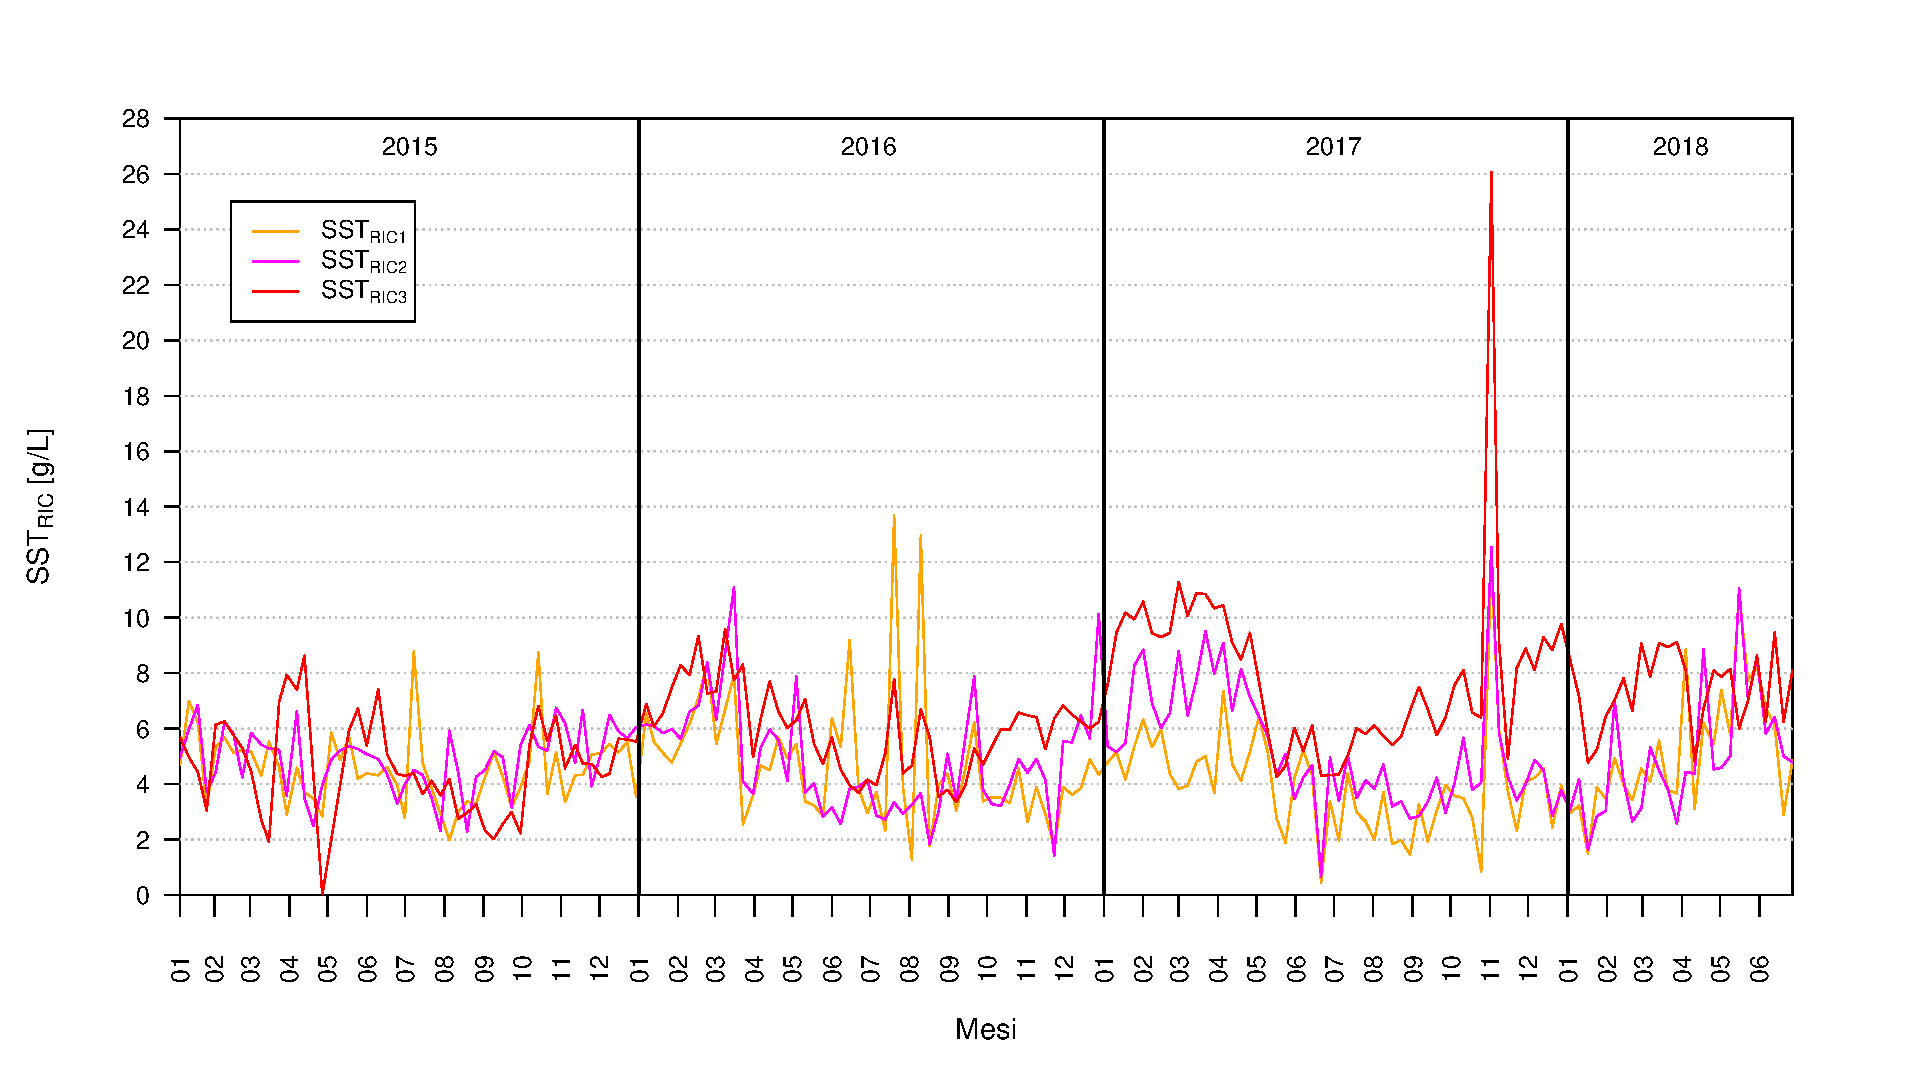
\includegraphics[width=\linewidth]{sa_SSTric}}	\centering
	\caption{Andamento della concentrazione di SST nel fango di ricircolo}
	\label{fig:sa_SSTric}
\end{figure}

Relativamente al volume del fango, tutte le linee sono caratterizzate da un andamento simile e presentano una grande variabilità nel tempo da cui sembra essere individuabile una certa periodicità (\autoref{fig:sa_SSS-SVI1}, \autoref{fig:sa_SSS-SVI2} e \autoref{fig:sa_SSS-SVI3}), correlabile, come noto, alle condizioni di carico e temperatura. 
Nelle medesime figure, è rappresentato lo SVI che, nelle prime due linee, segue l'andamento dei SSS, mentre nella terza non segue le oscillazioni ma si mantiene abbastanza stabile. In tutte le linee, molto frequentemente, viene superato il valore di 150 mL/g, soglia indicativa per stabilire se le caratteristiche di sedimentabilità del fango sono accettabili. In realtà, il valore dello SVI potrebbe essere fortemente influenzato dal fatto che è stato calcolato a partire da un fango molto voluminoso e quindi i valori ottenuti non sono particolarmente significativi (sarebbe stato meglio determinarli tramite diluizione).

\begin{figure}[H]
	\fbox{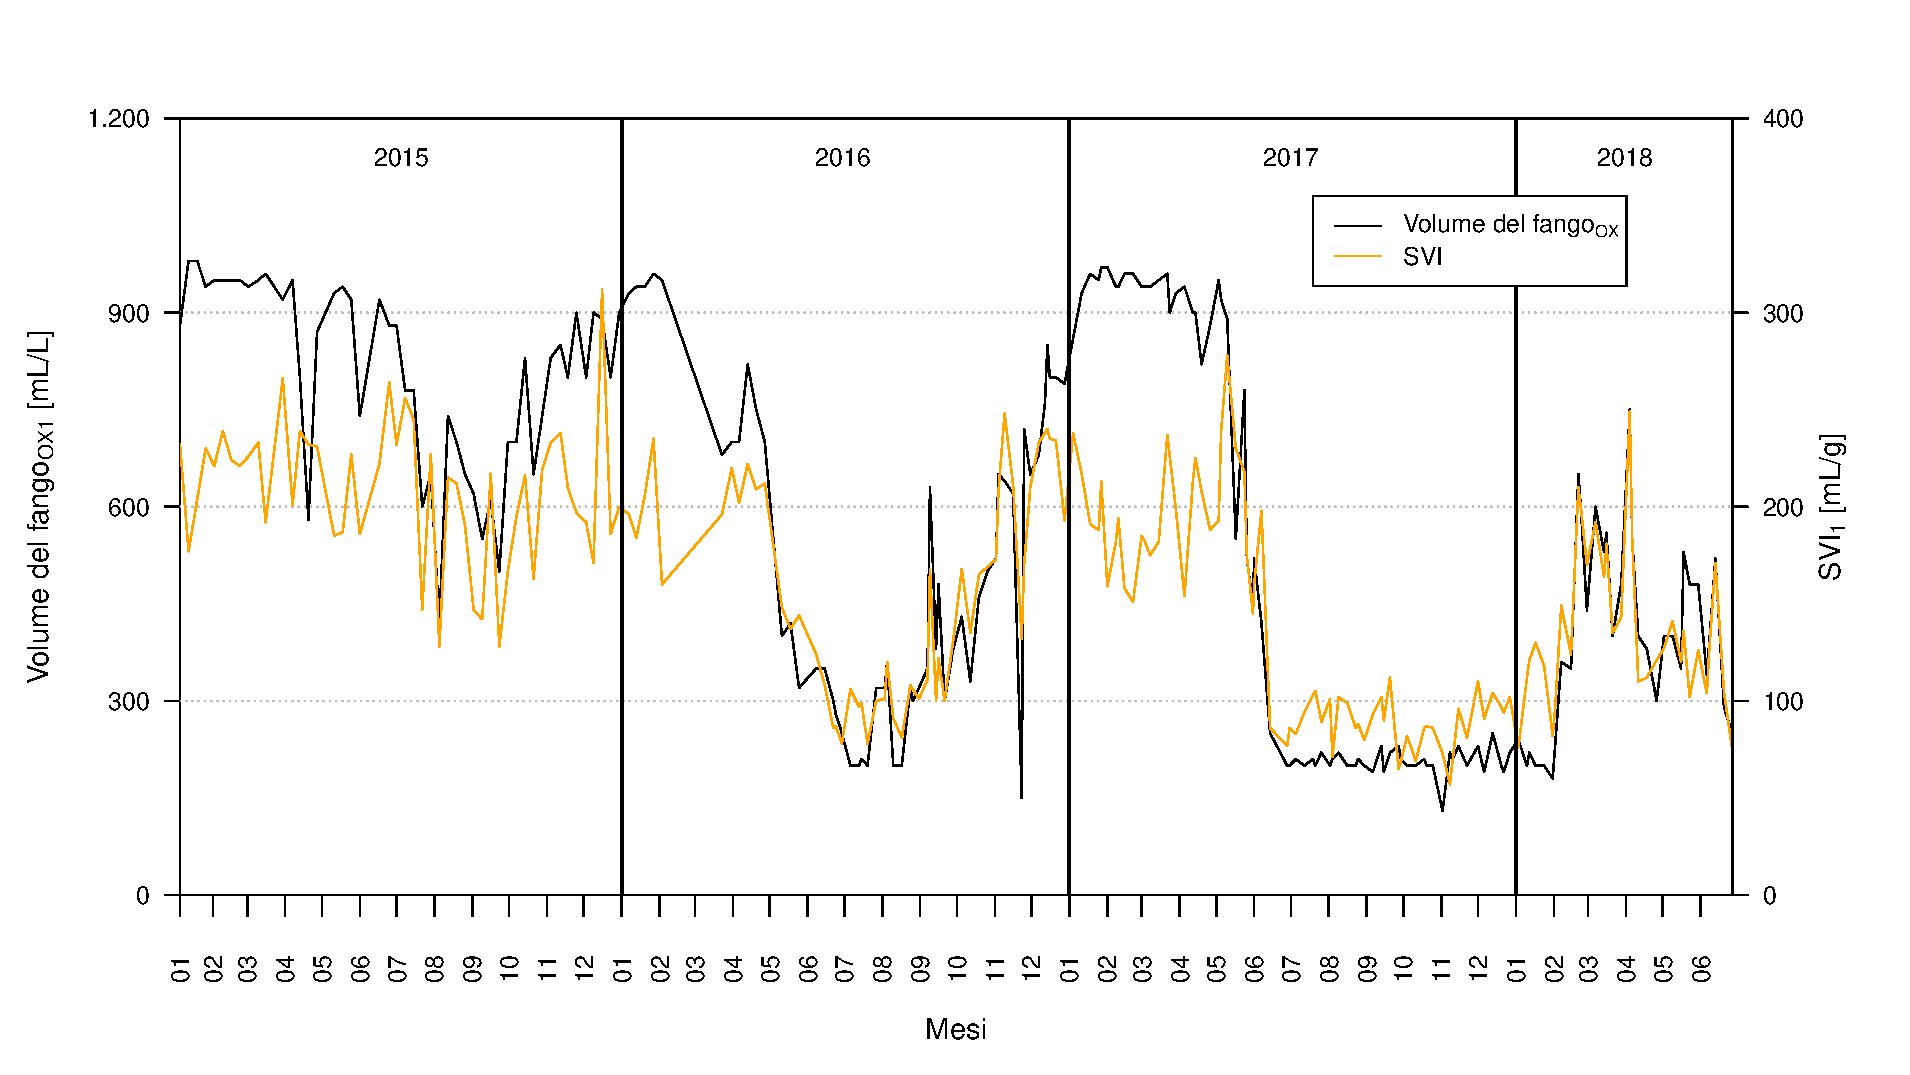
\includegraphics[width=\linewidth]{sa_SSS-SVI1}}	\centering
	\caption{Andamento del volume del fango e dello SVI nella vasca di ossidazione della linea 1}
	\label{fig:sa_SSS-SVI1}
\end{figure}
\begin{figure}[H]
	\fbox{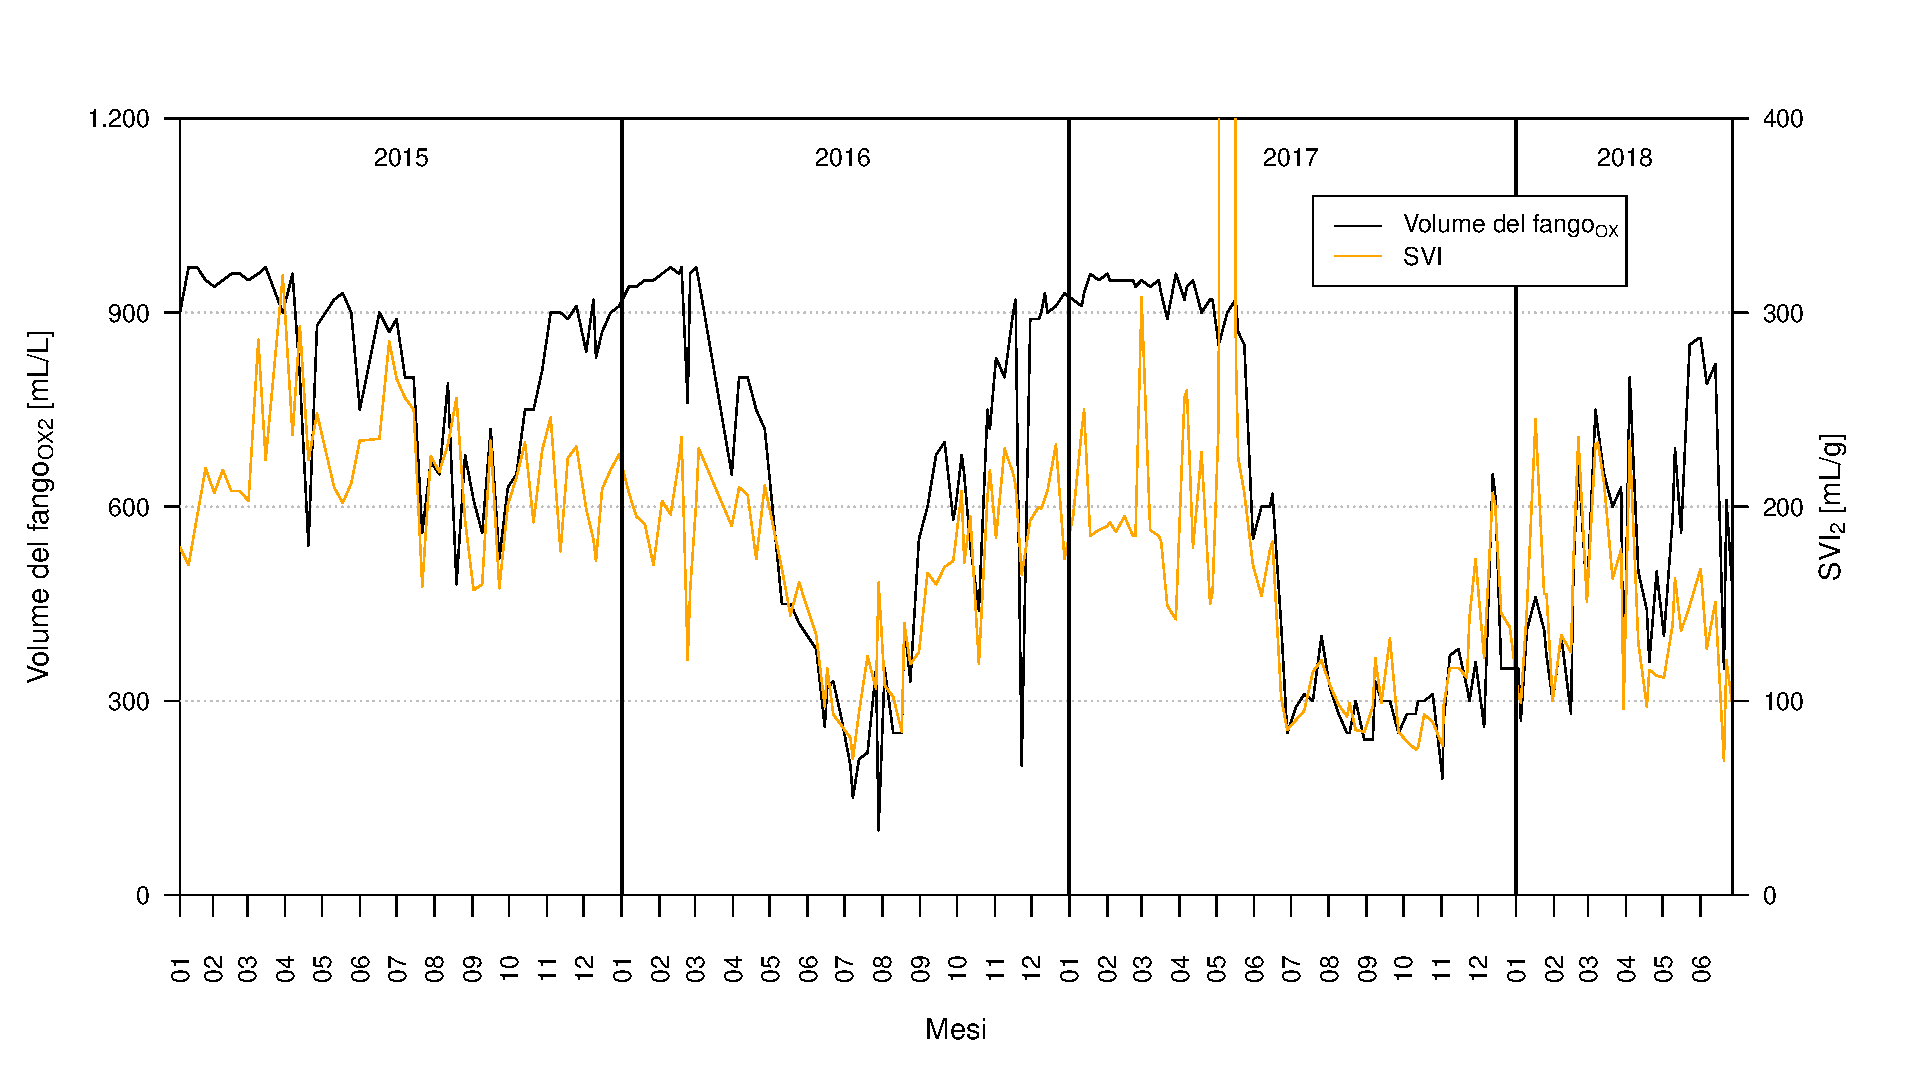
\includegraphics[width=\linewidth]{sa_SSS-SVI2}}	\centering
	\caption{Andamento del volume del fango e dello SVI nella vasca di ossidazione della linea 2}
	\label{fig:sa_SSS-SVI2}
\end{figure}
\begin{figure}[H]
	\fbox{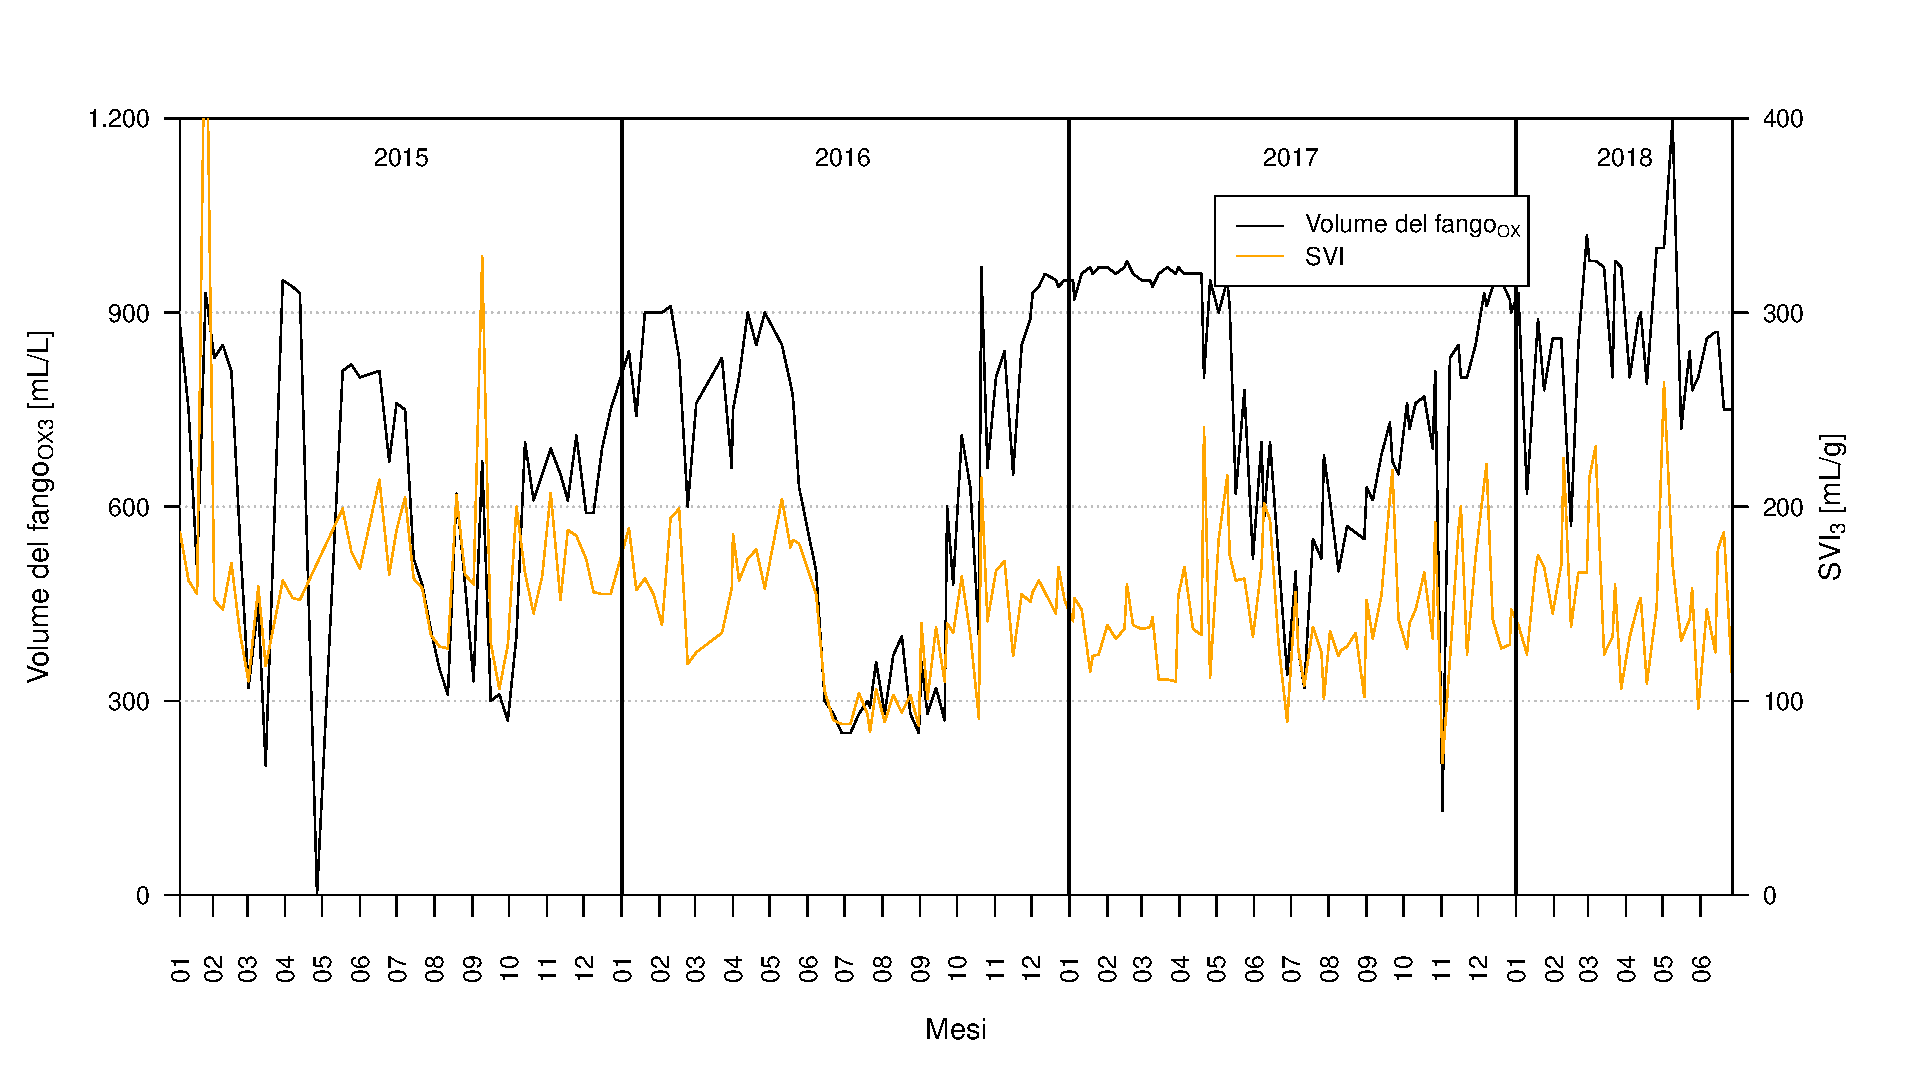
\includegraphics[width=\linewidth]{sa_SSS-SVI3}}	\centering
	\caption{Andamento del volume del fango e dello SVI nella vasca di ossidazione della linea 3}
	\label{fig:sa_SSS-SVI3}
\end{figure}

La portata del fango di supero, rappresentata in \autoref{fig:sa_Qf}, è variabile e ha una tendenza decrescente nel tempo. Si precisa che i numerosi valori pari a 0 m\textsuperscript{3}/d si hanno in corrispondenza di quei giorni in cui non si ha estrazione del fango di supero dal fondo del sedimentatore. In questo impianto non c'è un sistema di misurazione della portata di supero ma i valori derivano da una stima basata sul volume di riempimento della vasca e, quindi, sono affetti da notevole incertezza. Essa si propaga all'età del fango, per il calcolo della quale serve conoscere la portata del fango di supero.

\begin{figure}[H]
	\fbox{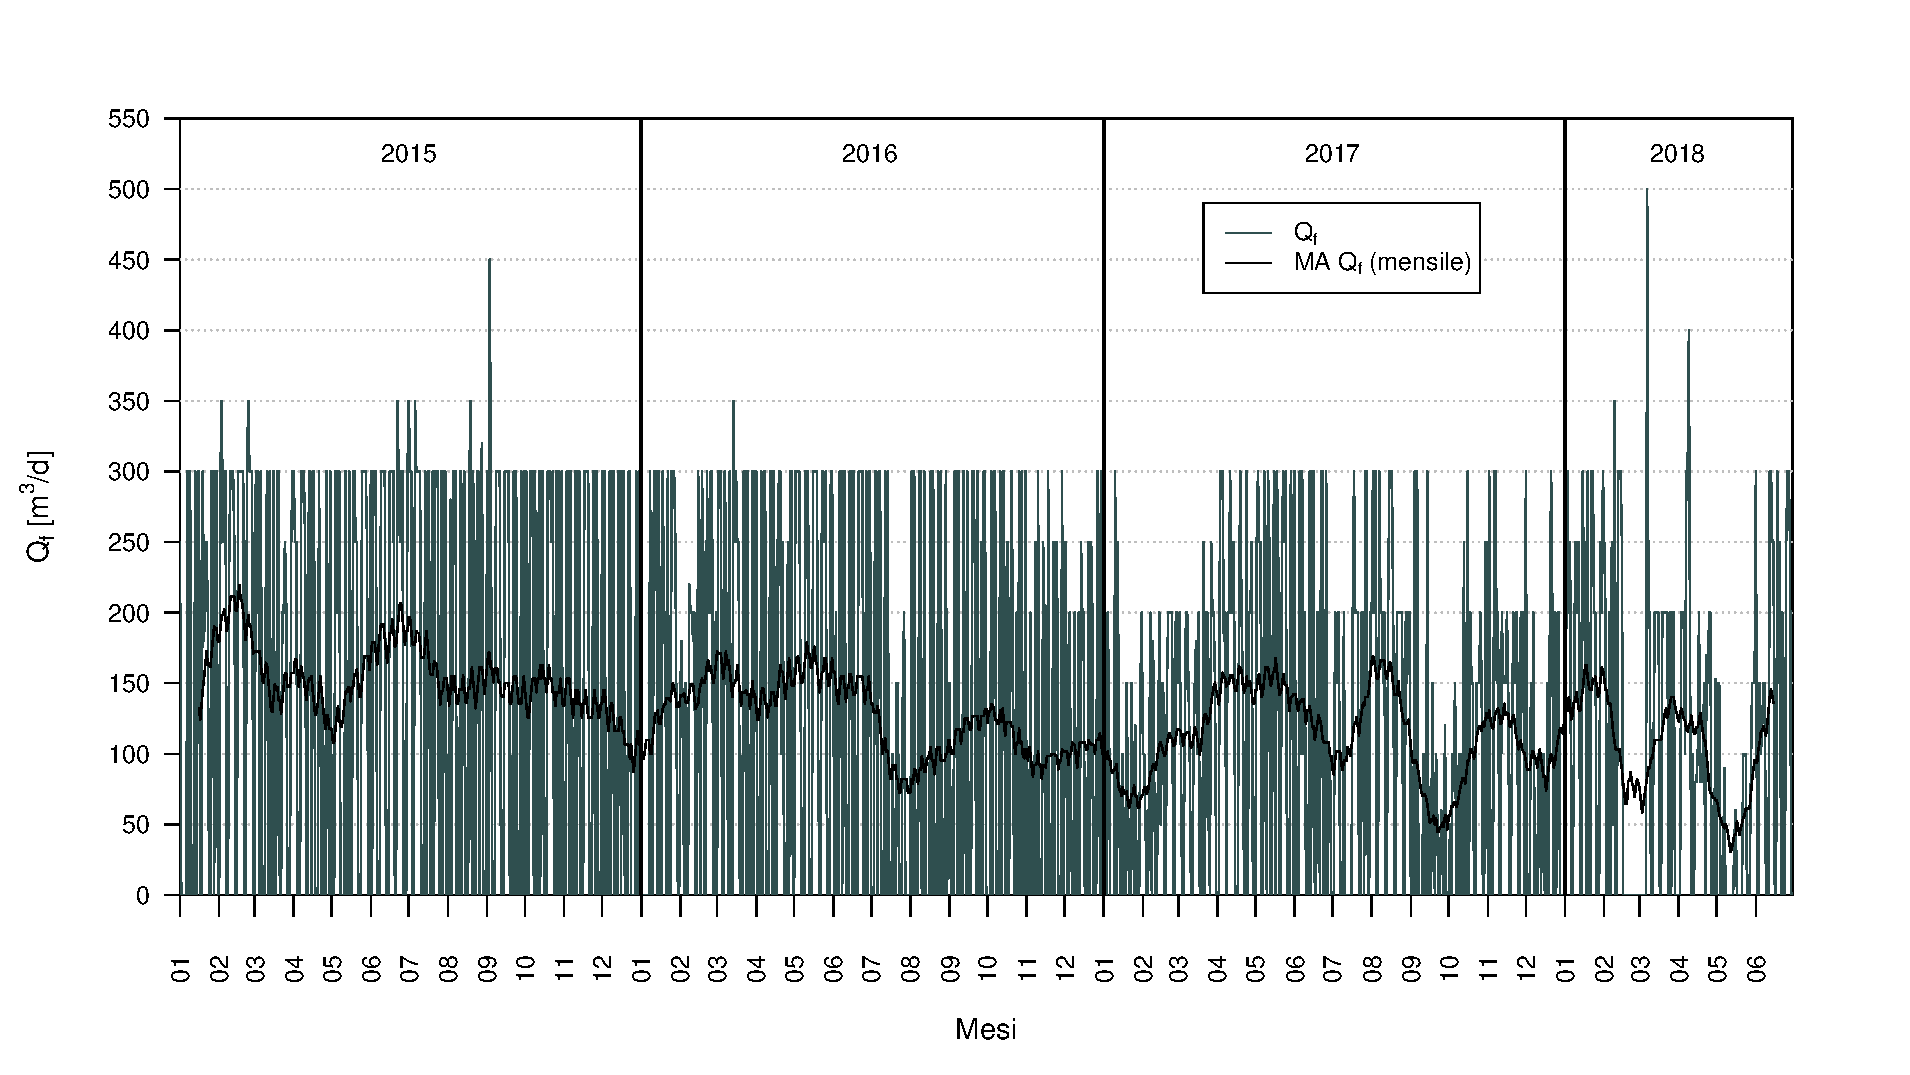
\includegraphics[width=\linewidth]{sa_Qf}}	\centering
	\caption{Andamento della portata del fango di supero}
	\label{fig:sa_Qf}
\end{figure}

Il carico del fango è generalmente basso (con media pari a 0,09 d\textsuperscript{-1}) ed è quindi favorita la nitrificazione (\autoref{fig:sa_Cf}). 
\begin{figure}[H]
	\fbox{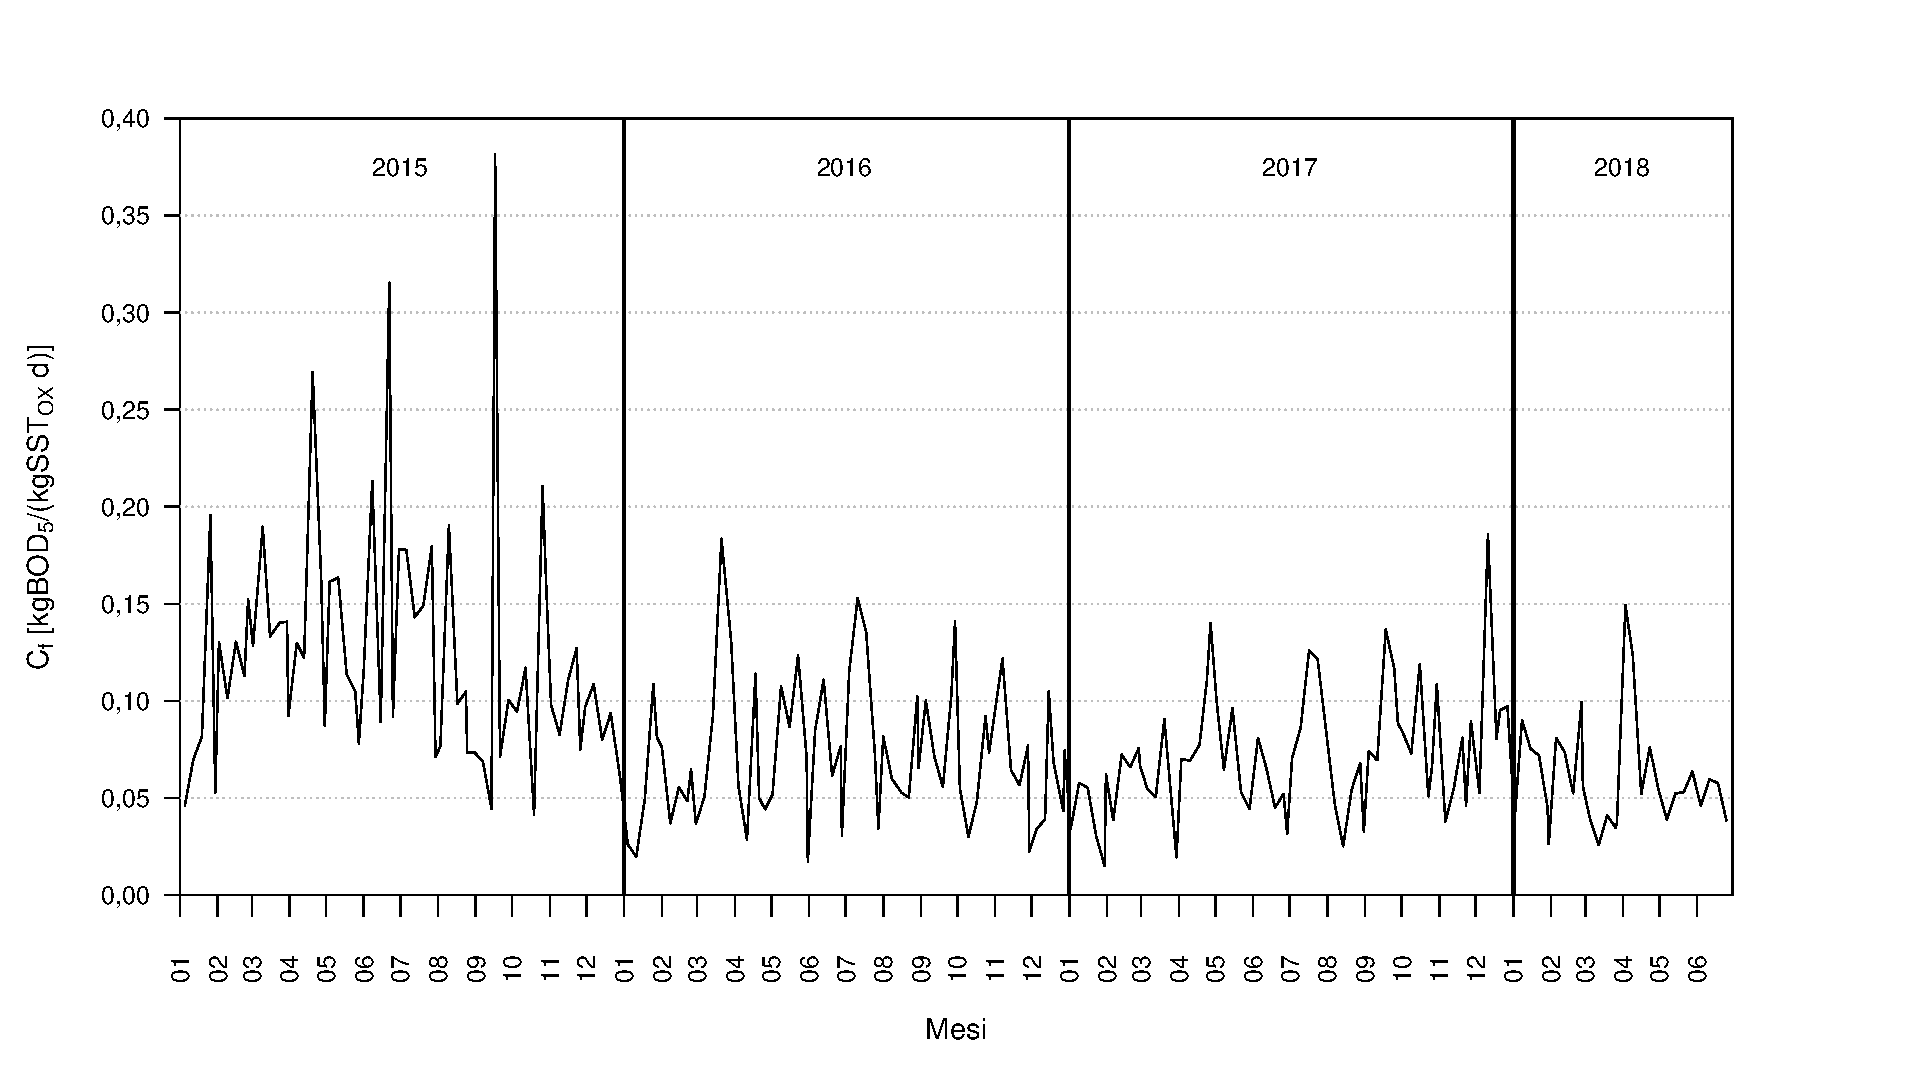
\includegraphics[width=\linewidth]{sa_Cf}}	\centering
	\caption{Andamento del carico del fango}
	\label{fig:sa_Cf}
\end{figure}
\begin{figure}[H]
	\fbox{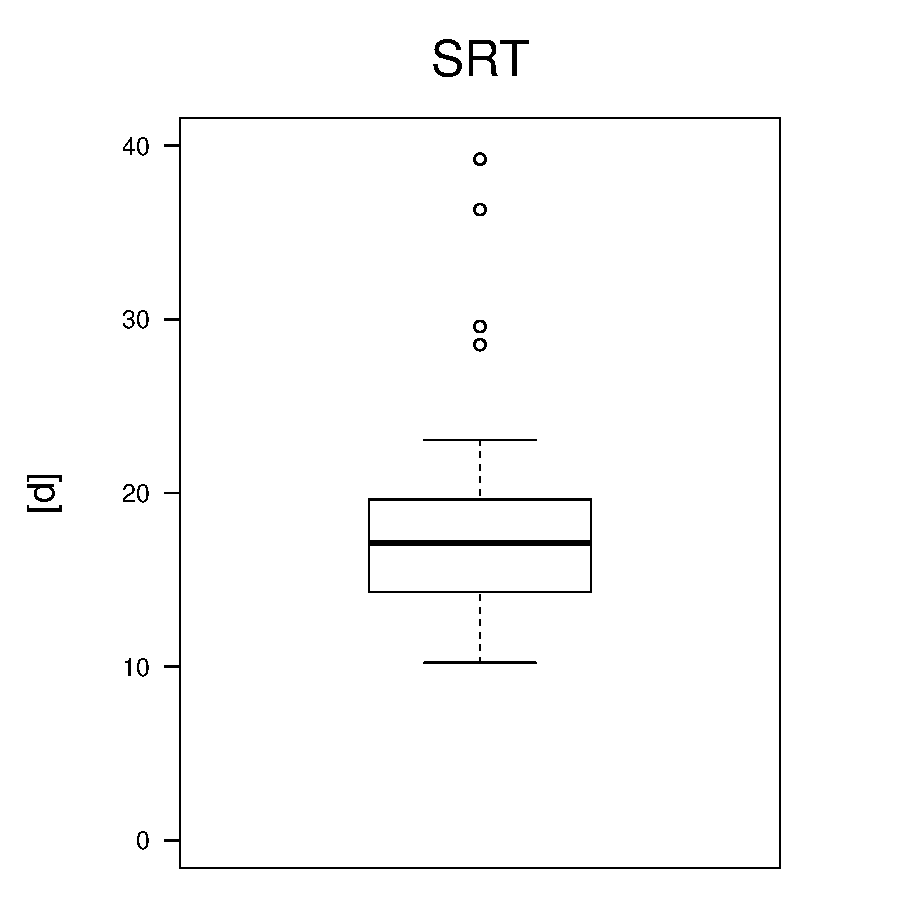
\includegraphics[width=\linewidth]{sa_SRT}}	\centering
	\caption{Andamento dell'età del fango (SRT)}
	\label{fig:sa_SRT}
\end{figure}

L'età del fango, mostrata in \autoref{fig:sa_SRT}, è variabile attorno a un valore medio di circa 18 giorni e quindi è possibile ottenere la completa rimozione dell'azoto per mezzo dei processi di nitrificazione e denitrificazione. Si può osservare un andamento crescente nel tempo.

La concentrazione di ossigeno disciolto nelle vasche di ossidazione delle linee 1 e 2 è piuttosto variabile da valori molto prossimi allo 0 fino a valori di saturazione (\autoref{fig:sa_OD1_2}). Da ottobre 2017 a giugno 2018 l'andamento è quello atteso in relazione alla temperatura, ovvero cresce nei mesi invernali e decresce via via che le temperature aumentano in primavera ed estate. Nel resto del 2017, invece, non si individua questo tipo di corrispondenza (ad esempio, a luglio e agosto si hanno concentrazioni maggiori di quelle di febbraio).

Nella linea 3, invece, la concentrazione di ossigeno disciolto in vasca di ossidazione è meno variabile, seppur in maniera ancora importante, ed è principalmente compresa tra 2,5 e 7,5 mg/L, senza mostrare un andamento dipendente dalla temperatura. A maggio e giugno 2018 si evidenzia un trend marcatamente crescente (\autoref{fig:sa_OD3}).
Il set point di 2 mg/L si tiene in poche casi poiché i compressori sono sovradimensionati e, di conseguenza, anche quando sono regolati al minimo, insufflano più aria del necessario.

\begin{figure}[H]
	\fbox{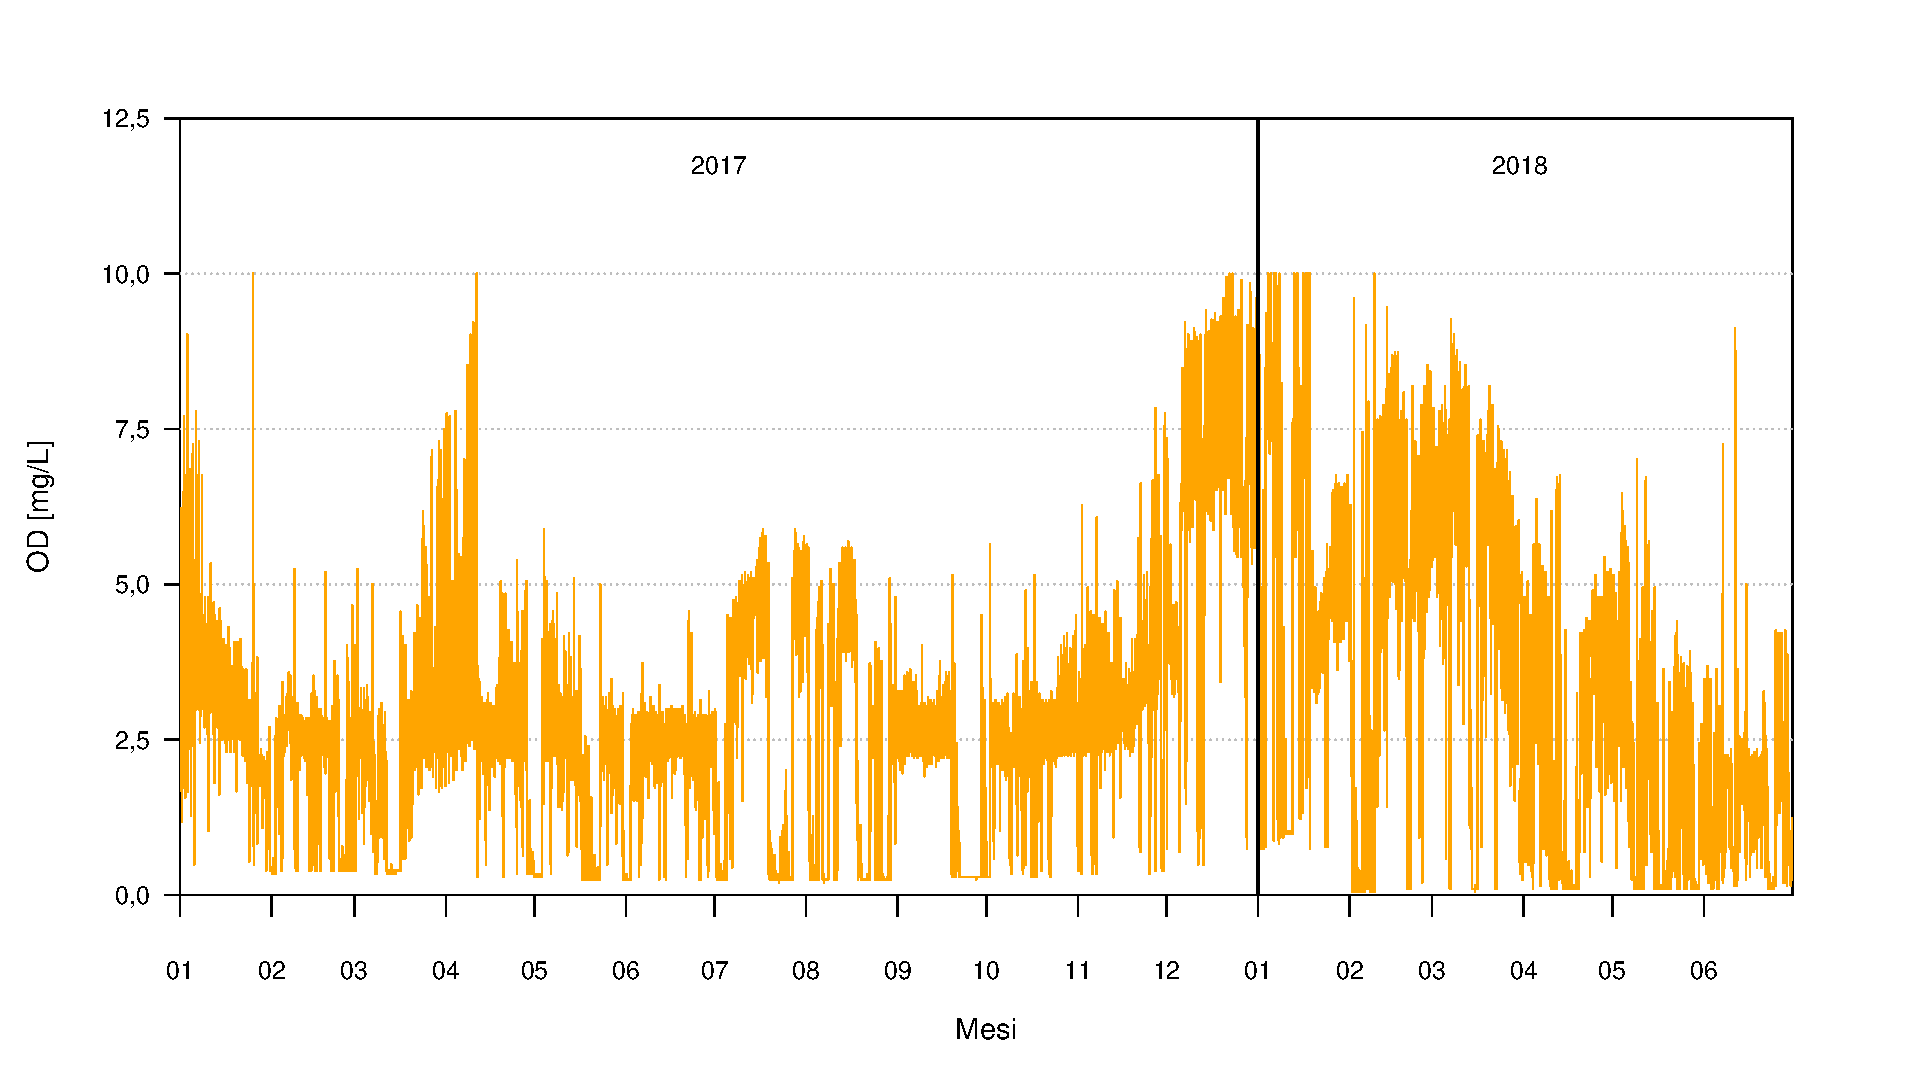
\includegraphics[width=\linewidth]{OD/sa_OD_linee1_2_tot}}	\centering
	\caption{Andamento della concentrazione di ossigeno disciolto in vasca di ossidazione - linee 1 e 2}
	\label{fig:sa_OD1_2}
\end{figure}
\begin{figure}[H]
	\fbox{\includegraphics[width=\linewidth]{OD/sa_OD_linea3_tot}}	\centering
	\caption{Andamento della concentrazione di ossigeno disciolto in vasca di ossidazione - linea 3}
	\label{fig:sa_OD3}
\end{figure}


\subsection{Impianto B}
\subsubsection{Caratteristiche del liquame in ingresso}

Il grafico di \autoref{fig:c_qin-prec} riporta l’andamento delle portate giornaliere in ingresso all’impianto e le precipitazioni mensili.
I valori di portata risultano piuttosto stabili ad esclusione dell’anno 2017, in cui la portata decresce rapidamente a inizio anno. Essa assume valori per lo più inferiori rispetto agli anni precedenti. Tra febbraio e marzo 2018, la portata aumenta e il suo valore medio si riavvicina a quello degli anni 2015 e 2016 (\autoref{tab:c_portate}).
Le precipitazioni mensili sono variabili e non sono correlate alla portata, che non sembra esserne influenzata. Nel 2017, periodo in cui la portata ha valore medio minore, le precipitazioni sono generalmente più abbondanti di quelle del 2015 e confrontabili (ad esclusione di alcuni mesi) con quelle del 2016. Pertanto, non si è in grado di indicare con esattezza le cause che inducono le variazioni di portata. 
Come valore di riferimento per la portata in tempo asciutto, si considera la mediana calcolata sull’intero arco temporale considerato, arrotondata al valore di 1.600 m\textsuperscript{3}/d. Tale valore rispetta la potenzialità di progetto di 2.000 m\textsuperscript{3}/d.
\begin{figure}[H]
	\fbox{\includegraphics[width=\linewidth]{c_qin-prec}}	\centering
	\caption{Andamento della portata giornaliera in ingresso e precipitazioni mensili}
	\label{fig:c_qin-prec}
\end{figure}
\begin {table}[H]
\scriptsize
\begin{center}
	\begin{tabular}{|>{\centering\arraybackslash}p{3,2cm}|>{\centering\arraybackslash}p{3,2cm}|>{\centering\arraybackslash}p{3,2cm}|>{\centering\arraybackslash}p{3,2cm}|}
		\hline 
		\textbf{Periodo} & \textbf{Media Q\textsubscript{IN} [m\textsuperscript{3}/d]} & \textbf{Mediana Q\textsubscript{IN} [m\textsuperscript{3}/d]} & \textbf{Media/Mediana [ - ]} \\ 
		\hline 
		2015 & 1.727 & 1.710 & 1,01 \\ 
		\hline 
		2016 & 1.712 & 1.685 & 1,02 \\ 
		\hline 
		2017 & 1.391 & 1.347 & 1,03 \\ 
		\hline 
		2018 & 1.612 & 1.525 & 1,06 \\ 
		\hline 
		2015 - 2018 & 1.610 & 1.567 & 1,03 \\ 
		\hline 
	\end{tabular} 
	\caption {Media, mediana e rapporto media/mediana delle portate in ingresso}
	\label{tab:c_portate}
\end{center}
\end{table}
\paragraph{Caratteristiche qualitative}

L’andamento delle concentrazioni di BOD\textsubscript{5} e COD ottenute attraverso il campionamento routinario è mostrato in \autoref{fig:c_BOD-COD}.
Entrambe le concentrazioni sono molto variabili, in particolar modo per quanto riguarda il COD. Il COD si mantiene, principalmente, nell'intervallo 500-1.500 mg/L (come media mobile), mentre il BOD\textsubscript{5} sta nell'intervallo 130-850 mg/L. Questi valori sono tipici di un liquame a concentrazione media-forte (\autoref{tab:conc_tipiche}).
Sia BOD\textsubscript{5} che COD manifestano un trend decrescente al passare del tempo. In generale si individua una certa correlazione tra le due grandezze. Tuttavia, ad aumenti notevoli di concentrazione di COD non sempre corrispondono aumenti equivalenti di BOD\textsubscript{5}.
A partire dal 2016 sembra esserci una certa periodicità che potrebbe essere legata a scarichi di allevamenti (sono in corso delle verifiche).
\begin{figure}[H]
	\fbox{\includegraphics[width=\linewidth]{c_BOD-COD}}	\centering
	\caption{Andamento delle concentrazioni in ingresso di BOD\textsubscript{5} e COD}
	\label{fig:c_BOD-COD}
\end{figure}
\begin{figure}[H]
	\fbox{\includegraphics[width=\linewidth]{c_BOD-1q}}	\centering
	\caption{Andamento della concentrazione in ingresso di BOD\textsubscript{5} e dell'inverso della portata giornaliera}
	\label{fig:c_BOD-1q}
\end{figure}
I grafici di \autoref{fig:c_COD-1q} e \autoref{fig:c_BOD-1q} riportano i valori di concentrazione di COD e BOD\textsubscript{5} rispetto all’inverso della portata giornaliera al fine di verificare se le variazioni di concentrazione siano correlate alla portata.
In entrambi i casi non si individua correlazione tra concentrazione e portata. Infatti, spesso, negli intervalli in cui la portata diminuisce (e quindi 1/Q aumenta), la concentrazione diminuisce e viceversa.
\begin{figure}[H]
	\fbox{\includegraphics[width=\linewidth]{c_COD-1q}}	\centering
	\caption{Andamento della concentrazione in ingresso di COD e dell'inverso della portata giornaliera}
	\label{fig:c_COD-1q}
\end{figure}


In \autoref{fig:c_COD-SST} è mostrato l’andamento della concentrazione di COD e di SST e si vede chiaramente che c’è correlazione tra le due grandezze (a inizio 2017 non è molto marcata).

Nel grafico di \autoref{fig:c_BOD-SST}, invece, si ha il confronto tra BOD\textsubscript{5} e SST che individua ancora correlazione, anche se non così buona come per il COD.
Di conseguenza, poiché nell’analisi del grafico di \autoref{fig:c_BOD-COD} si era individuata una tendenza alla diminuzione delle concentrazioni di COD e BOD\textsubscript{5}, essendo essi correlati ai SST, anche questi ultimi hanno un trend decrescente, come è ben visibile nella rappresentazione grafica.

\begin{figure}[H]
	\fbox{\includegraphics[width=\linewidth]{c_COD-SST}}	\centering
	\caption{Andamento delle concentrazioni in ingresso di COD e SST}
	\label{fig:c_COD-SST}
\end{figure}
\begin{figure}[H]
	\fbox{\includegraphics[width=\linewidth]{c_BOD-SST}}	\centering
	\caption{Andamento delle concentrazioni in ingresso di BOD\textsubscript{5} e di SST}
	\label{fig:c_BOD-SST}
\end{figure}

Si riporta ora l’andamento dell’azoto totale e dell’azoto ammoniacale (\autoref{fig:c_Ntot-NNH4+}).
Entrambe le grandezze sono notevolmente variabili e in alcuni casi superano i valori di 85 mg/L per l’azoto totale e 50 mg/L per quello ammoniacale, tipici di un liquame domestico fortemente concentrato (\autoref{tab:conc_tipiche}). Ciò potrebbe dipendere, come già visto anche per il COD, dalla presenza di scarichi di diverso tipo rispetto a quelli urbani.
L’azoto totale è prevalentemente costituito da azoto ammoniacale (mediamente il 67\%), come previsto per un refluo di origine civile, anche se in alcuni mesi del 2015 e del 2016 la sua percentuale rispetto al totale diminuisce.
L’azoto totale sembra avere un trend leggermente decrescente, mentre l’azoto ammoniacale non esibisce particolari tendenze.
\begin{figure}[H]
	\fbox{\includegraphics[width=\linewidth]{c_Ntot-NNH4+}}	\centering
	\caption{Andamento delle concentrazioni in ingresso di azoto totale e azoto ammoniacale}
	\label{fig:c_Ntot-NNH4+}
\end{figure}
Le concentrazioni dell’azoto nitroso e dell’azoto nitrico (\autoref{fig:c_NO2-NO3}) sono irrisorie, come ci si aspetta per liquami di origine domestica. Infatti, le forme azotate ossidate non superano mai i 2,5 mg/L, mentre il valore medio della concentrazione di azoto totale è di circa 60 mg/L.
\begin{figure}[H]
	\fbox{\includegraphics[width=\linewidth]{c_NO2-NO3}}	\centering
	\caption{Andamento delle concentrazioni in ingresso di azoto nitroso e azoto nitrico}
	\label{fig:c_NO2-NO3}
\end{figure}
\begin{figure}[H]
	\fbox{\includegraphics[width=\linewidth]{c_Ntot-1q}}	\centering
	\caption{Andamento delle concentrazioni in ingresso di azoto totale e dell'inverso della portata giornaliera}
	\label{fig:c_Ntot-1q}
\end{figure}

Come per il COD, anche nel caso delle concentrazioni di azoto totale non si manifesta alcuna correlazione con l'inverso della portata giornaliera e quindi non è possibile trovare corrispondenza tra la variazione di portata e di concentrazione di azoto totale (\autoref{fig:c_Ntot-1q}).

Il grafico di \autoref{fig:c_Ptot} mostra le oscillazioni della concentrazione di fosforo totale in ingresso all’impianto.
In più occasioni, la concentrazione supera i 10 mg/L (valore di riferimento per un refluo di origine civile fortemente concentrato, si veda la \autoref{tab:conc_tipiche}) e quindi è ancora valida l’ipotesi di scarichi di tipo diverso.
Nel corso del tempo, si individua un andamento decrescente.\\

\begin{figure}[H]
	\fbox{\includegraphics[width=\linewidth]{c_Ptot}}	\centering
	\caption{Andamento della concentrazione in ingresso di fosforo totale}
	\label{fig:c_Ptot}
\end{figure}

Di seguito sono stati analizzati i valori dei rapporti tra le concentrazioni dei diversi inquinanti e sono stati confrontati con i valori di riferimento per un liquame urbano presentati in \autoref{tab:ppc_rapporti}.

Il rapporto tra BOD\textsubscript{5} e COD è mostrato in \autoref{fig:c_BOD_COD}.
Tale rapporto è molto variabile e, nonostante abbia media pari a 0,44, spesso è al di sotto del valore minimo per un liquame urbano. Una possibile spiegazione è data dalla presenza di scarichi industriali o di allevamenti.
Facendo un confronto con l’andamento del COD, si nota che, in coincidenza dei picchi di quest’ultimo, il rapporto assume valori minimi. Questo conferma quanto constatato per il grafico di \autoref{fig:c_BOD-COD}, ovvero che, quando il COD cresce particolarmente, il BOD\textsubscript{5} non asseconda l’andamento.\\

\begin{figure}[H]
	\fbox{\includegraphics[width=\linewidth]{c_BOD_COD}}	\centering
	\caption{Andamento del rapporto tra BOD\textsubscript{5} e COD in ingresso}
	\label{fig:c_BOD_COD}
\end{figure}

La \autoref{fig:c_Ntot_BOD-Ntot_COD} mostra  gli andamenti dei rapporti tra azoto totale e BOD\textsubscript{5} e azoto totale e COD, che sono abbastanza simili.
Il rapporto N\textsubscript{tot}/BOD\textsubscript{5} (\autoref{fig:c_Ntot_BOD}) è molto variabile e quindi non c’è correlazione tra le due grandezze. Esso risente principalmente del trend decrescente osservato per il BOD\textsubscript{5} (\autoref{fig:c_BOD-COD}) mentre è meno influenzato dall’andamento decrescente dell’azoto totale (\autoref{fig:c_Ntot-NNH4+}). Come conseguenza, il rapporto tende ad aumentare. Nonostante la maggior parte delle misurazioni si trovi al di sotto del valore minimo tipico di un liquame urbano, la media risulta al di sopra di tale valore, spostata verso il valore tipico.
Il rapporto N\textsubscript{tot}/COD assume valori variabili e, per le medesime considerazioni fatte per il rapporto N\textsubscript{tot}/BOD\textsubscript{5}, si osserva un trend crescente (\autoref{fig:c_Ntot_COD}). Quasi tutti i dati giacciono al di sotto del valore minimo caratteristico di un liquame urbano e, di conseguenza, anche la media è posizionata al di sotto di tale valore.

\begin{figure}[H]
	\fbox{\includegraphics[width=\linewidth]{c_Ntot_BOD-Ntot_COD}}	\centering
	\caption{Andamento dei rapporti tra azoto totale e BOD\textsubscript{5} e azoto totale e COD in ingresso}
	\label{fig:c_Ntot_BOD-Ntot_COD}
\end{figure}
\begin{figure}[H]
	\fbox{\includegraphics[width=\linewidth]{c_Ntot_BOD}}	\centering
	\caption{Andamento del rapporto tra azoto totale e BOD\textsubscript{5} in ingresso}
	\label{fig:c_Ntot_BOD}
\end{figure}
\begin{figure}[H]
	\fbox{\includegraphics[width=\linewidth]{c_Ntot_COD}}	\centering
	\caption{Andamento del rapporto tra azoto totale e COD in ingresso}
	\label{fig:c_Ntot_COD}
\end{figure}
\begin{figure}[H]
	\fbox{\includegraphics[width=\linewidth]{c_Ptot_BOD-Ptot_COD}}	\centering
	\caption{Andamento dei rapporti tra fosforo totale e BOD\textsubscript{5} e fosforo totale e COD in ingresso}
	\label{fig:c_Ptot_BOD-Ptot_COD}
\end{figure}
\begin{figure}[H]
	\fbox{\includegraphics[width=\linewidth]{c_Ptot_BOD}}	\centering
	\caption{Andamento del rapporto tra fosforo totale e BOD\textsubscript{5} in ingresso}
	\label{fig:c_Ptot_BOD}
\end{figure}
\begin{figure}[H]
	\fbox{\includegraphics[width=\linewidth]{c_Ptot_COD}}	\centering
	\caption{Andamento del rapporto tra fosforo totale e COD in ingresso}
	\label{fig:c_Ptot_COD}
\end{figure}

Nel grafico di \autoref{fig:c_Ptot_BOD-Ptot_COD} sono rappresentati i rapporti tra fosforo e BOD\textsubscript{5} e fosforo e COD e si osserva correlazione.
L’andamento variabile porta alla conclusione che non ci sia correlazione tra la concentrazione di fosforo e quella di BOD\textsubscript{5} e COD.
Nel caso del rapporto tra fosforo totale e BOD\textsubscript{5}, si nota che la media è sbilanciata verso il valore massimo atteso per liquami urbani (\autoref{fig:c_Ptot_BOD}).
Nel caso del rapporto tra fosforo totale e COD, invece, la media è di poco superiore al valore tipico per liquami urbani (\autoref{fig:c_Ptot_COD}).

\begin{figure}[H]
	\fbox{\includegraphics[width=\linewidth]{c_Ptot_Ntot}}	\centering
	\caption{Andamento del rapporto tra fosforo totale e azoto totale in ingresso}
	\label{fig:c_Ptot_Ntot}
\end{figure}

Il rapporto tra fosforo totale e azoto totale è molto variabile e la sua media supera il valore massimo per un liquame urbano (\autoref{fig:c_Ptot_Ntot}).

In \autoref{tab:c_rapporti} sono raccolti i valori medi dei rapporti calcolati e i rispettivi valori tipici per liquami urbani. Si osserva che le caratteristiche del liquame sono sbilanciate verso il fosforo.\\

\begin{table}[H]
	\scriptsize
	\begin{center}
		\begin{tabular}{|>{\centering\arraybackslash}p{3cm}|>{\centering\arraybackslash}p{3cm}|>{\centering\arraybackslash}p{3cm}|}
			\hline 
			\textbf{Rapporto} & \textbf{Media} & \textbf{Valore tipico} \\ 
			\hline 
			BOD\textsubscript{5}/COD & 0,44 & 0,50 \\ 
			\hline 
			N\textsubscript{tot}/BOD\textsubscript{5} & 0,19 & 0,20 \\ 
			\hline 
			N\textsubscript{tot}/COD & 0,08 & 0,10 \\ 
			\hline 
			P\textsubscript{tot}/BOD\textsubscript{5} & 0,026 & 0,020 \\ 
			\hline 
			P\textsubscript{tot}/COD & 0,011 & 0,010 \\ 
			\hline 
			P\textsubscript{tot}/N\textsubscript{tot} & 0,14 & 0,10 \\ 
			\hline 
		\end{tabular} 
		\caption{Valori medi calcolati e  valori tipici per un liquame urbano dei rapporti significativi tra le concentrazioni di inquinanti in ingresso}
		\label{tab:c_rapporti}
	\end{center}	
\end{table}	

\begin{figure}
	\fbox{\includegraphics[width=\linewidth]{c_EC}}	\centering
	\caption{Andamento della concentrazione in ingresso di \textit{Escherichia coli}}
	\label{fig:c_EC}
\end{figure}

La concentrazione di carica batterica in termini di \textit{Escherichia coli} è rappresentata in \autoref{fig:c_EC} dove è evidente un trend crescente.

\begin{figure}
	\fbox{\includegraphics[width=\linewidth]{c_pH}}	\centering
	\caption{Andamento del pH del liquame in ingresso}
	\label{fig:c_pH}
\end{figure}

Le misurazioni di pH hanno valore medio 7,7 e, in alcuni periodi del 2018, superano il valore 8 (\autoref{fig:c_pH}). In un caso isolato nel 2016 si raggiunge anche il valore 9. Si può osservare un trend crescente.
\begin{figure}
	\fbox{\includegraphics[width=\linewidth]{c_T}}	\centering
	\caption{Andamento della temperatura del liquame in ingresso}
	\label{fig:c_T}
\end{figure}

La temperatura del refluo in ingresso presenta le classiche variazioni stagionali (\autoref{fig:c_T}).
Si osservano valori minimi di circa 10\textdegree C e valori massimi compresi tra 25 e 28\textdegree C.

\paragraph{{Carichi inquinanti}}

Come per l'impianto A, a partire dai dati di concentrazione e da quelli di portata, è stato possibile calcolare i carichi degli inquinanti in ingresso all'impianto.

I carichi di BOD\textsubscript{5} (\autoref{fig:c_car_BOD}) e di COD (\autoref{fig:c_COD_T}) ricalcano l'andamento decrescente delle loro rispettive concentrazioni. Per il calcolo dei carichi, infatti, si moltiplicano le concentrazioni per il valore di portata che, in questo caso, è piuttosto stabile.
Negli anni 2015 e 2016, questi carichi aumentano e diminuiscono in accordo con la temperatura del liquame in ingresso. Nel 2017, invece, essi assumono valori bassi nei mesi più caldi dell'anno.

\begin{figure}[H]
	\fbox{\includegraphics[width=\linewidth]{c_car_BOD}}	\centering
	\caption{Andamento del carico in ingresso di BOD\textsubscript{5} e della temperatura del liquame in ingresso}
	\label{fig:c_car_BOD}
\end{figure}
\begin{figure}[H]
	\fbox{\includegraphics[width=\linewidth]{c_COD_T}}	\centering
	\caption{Andamento del carico in ingresso di COD e della temperatura del liquame in ingresso}
	\label{fig:c_COD_T}
\end{figure}

La \autoref{fig:c_CODsup} mostra la distribuzione di frequenza dei carichi di COD e di BOD\textsubscript{5} e i percentili 90°, 75° e 50°.

\begin{figure}[H]
	\fbox{\includegraphics[width=\linewidth]{c_CODsup}}	\centering
	\caption{Distribuzione di frequenza dei carichi giornalieri in ingresso di COD e di BOD\textsubscript{5}}
	\label{fig:c_CODsup}
\end{figure}
\begin{figure}[H]
	\fbox{\includegraphics[width=\linewidth]{c_car_Ntot}}	\centering
	\caption{Andamento del carico in ingresso di azoto totale}
	\label{fig:c_car_Ntot}
\end{figure}

Il carico di azoto totale (\autoref{fig:c_car_Ntot}) e quello di fosforo totale (\autoref{fig:c_car_Ptot}) hanno un andamento che rispecchia quello delle concentrazioni piuttosto che quello dalle portate. In entrambi i casi si nota un trend leggermente decrescente.

\begin{figure}[H]
	\fbox{\includegraphics[width=\linewidth]{c_car_Ptot}}	\centering
	\caption{Andamento del carico in ingresso di fosforo totale}
	\label{fig:c_car_Ptot}
\end{figure}

Per completare l'analisi dei carichi, sono stati calcolati i carichi medi di BOD\textsubscript{5}, COD, azoto totale e fosforo totale, espressi in abitanti equivalenti (\autoref{subsec:carichi}). I risultati per l'intero periodo 2015 - 2018 e quelli su base annua sono rappresentati rispettivamente in \autoref{fig:c_AEtot} e \autoref{fig:c_AEanni}.
L'analisi sull'intero periodo evidenzia che la potenzialità di progetto di 10.000 abitanti equivalenti è sufficiente per il BOD\textsubscript{5} e l'azoto totale, mentre risulta leggermente superata dai carichi, in abitanti equivalenti, di COD e fosforo totale. Dalla valutazione condotta sulla media annua si osserva una progressiva decrescita nel tempo. Il 2015 presenta, per tutti gli inquinanti, valori significativamente eccedenti la potenzialità di progetto mentre nel 2016 tale condizione si verifica solo per COD e fosforo totale. Negli anni successivi, invece, tutti i parametri risultano essere compatibili con la potenzialità dell'impianto. Anche osservando il 90° percentile per il BOD\textsubscript{5} e il 92° percentile per il COD, i valori ottenuti sono sempre al di sopra della potenzialità di progetto (ad eccezione del BOD\textsubscript{5} nell'anno 2018). Come per l'impianto A, si sono valutati proprio questi due percentili perché, secondo quanto spiegato nella \autoref{sec:limiti_scarico}, è consentito eccedere la potenzialità di progetto nel 10\% dei giorni per il BOD\textsubscript{5} e nell'8\% per il COD\footnote{Per l'anno 2018 si è stimato che, a fine anno, si avrà un numero di misurazioni doppio rispetto a quello conteggiato a fine giugno, assumendo che la media dei carichi sul primo semestre sia rappresentativa di quella annuale. Ovviamente questa analisi andrà ripetuta a fine anno, quando si sarà in possesso di tutti i dati.}.

\begin{figure}[H]
	\fbox{\includegraphics[width=\linewidth]{c_AEtot}}	\centering
	\caption{Carichi medi in ingresso di BOD\textsubscript{5} (60 g ab\textsuperscript{-1} d\textsuperscript{-1}), COD (120 g ab\textsuperscript{-1} d\textsuperscript{-1}), azoto totale (12 g ab\textsuperscript{-1} d\textsuperscript{-1}) e fosforo totale (1,2 g ab\textsuperscript{-1} d\textsuperscript{-1}), espressi in abitanti equivalenti, calcolati sull'intero periodo 2015 - 2018}
	\label{fig:c_AEtot}
\end{figure}
\begin{figure}[H]
	\fbox{\includegraphics[width=\linewidth]{c_AEanni}}	\centering
	\caption{Carichi medi in ingresso di BOD\textsubscript{5} (60 g ab\textsuperscript{-1} d\textsuperscript{-1}), COD (120 g ab\textsuperscript{-1} d\textsuperscript{-1}), azoto totale (12 g ab\textsuperscript{-1} d\textsuperscript{-1}) e fosforo totale (1,2 g ab\textsuperscript{-1} d\textsuperscript{-1}), espressi in abitanti equivalenti, calcolati per ciascun anno}
	\label{fig:c_AEanni}
\end{figure}

\subsubsection{Caratteristiche dell'effluente}

Le caratteristiche dell'effluente devono rispettare i limiti allo scarico elencati in \autoref{tab:c_limiti}.

\paragraph{Caratteristiche qualitative}

Il grafico di \autoref{fig:c_BODout} rappresenta i valori di BOD\textsubscript{5} in ingresso e in uscita.
Per tutto il periodo considerato, la concentrazione di BOD\textsubscript{5} in uscita rispetta il limite di 20 mg/L. Essa è pressoché costante (attorno a in valore medio di 7,6 mg/L), ad eccezione di alcuni picchi che si mantengono comunque al di sotto del limite. 
Non si osserva correlazione tra la concentrazione in ingresso e quella in uscita.
\begin{figure}[H]
	\fbox{\includegraphics[width=\linewidth]{c_BODout}}	\centering
	\caption{Andamento delle concentrazioni di BOD\textsubscript{5} in ingresso e in uscita}
	\label{fig:c_BODout}
\end{figure}
\begin{figure}[H]
	\fbox{\includegraphics[width=\linewidth]{c_CODout}}	\centering
	\caption{Andamento delle concentrazioni di COD in ingresso e in uscita}
	\label{fig:c_CODout}
\end{figure}

I valori di COD in ingresso e in uscita sono rappresentati in \autoref{fig:c_CODout}.
Per tutto il periodo esaminato, la concentrazione di COD in uscita rispetta il limite di 100 mg/L con ampio margine ed è pressoché costante (in media pari a 20 mg/L).
Non si evidenzia correlazione tra concentrazione in ingresso e concentrazione in uscita.

Per quanto riguarda i SST, durante l’intero arco temporale considerato, la concentrazione in uscita rispetta il limite di 35 mg/L con ampio margine, ad eccezione di alcuni picchi che si mantengono comunque al di sotto del limite. Tale concentrazione è pressoché costante, in media 7,7 mg/L (\autoref{fig:c_SSTout-1q}).

Confrontando l’andamento della concentrazione di SST con la portata effluente, sembrerebbe che, esclusivamente in alcuni intervalli, la concentrazione di SST in uscita segua l'andamento della portata in uscita. In ogni caso, anche se ci fosse effetto di trascinamento, la concentrazione di inquinante in uscita si mantiene sempre al di sotto del limite allo scarico.
\begin{figure}[H]
	\fbox{\includegraphics[width=\linewidth]{c_SSTout-1q}}	\centering
	\caption{Andamento della concentrazione di SST in uscita e della portata effluente}
	\label{fig:c_SSTout-1q}
\end{figure}
\begin{figure}[H]
	\fbox{\includegraphics[width=\linewidth]{c_Ntotout}}	\centering
	\caption{Andamento delle concentrazioni di azoto totale in  ingresso e in uscita}
	\label{fig:c_Ntotout}
\end{figure}

Dalla rappresentazione delle concentrazioni in ingresso e in uscita, si ricava un’idea generale dell’efficacia di rimozione complessiva di azoto totale, che si può ritenere soddisfacente (\autoref{fig:c_Ntotout}). Infatti, ad eccezione di rari casi, il limite di 15 mg/L è sempre rispettato. Non c’è correlazione tra la concentrazione in ingresso e quella in uscita.

\begin{figure}[H]
	\fbox{\includegraphics[width=\linewidth]{c_NH4-NO2-NO3out}}	\centering
	\caption{Andamento delle concentrazioni in uscita di azoto ammoniacale, azoto nitroso e azoto nitrico}
	\label{fig:c_NH4-NO2-NO3out}
\end{figure}

Nella \autoref{fig:c_NH4-NO2-NO3out} sono rappresentati gli andamenti delle concentrazioni in uscita di azoto ammoniacale (N-NH\textsubscript{4}\textsuperscript{+}), azoto nitroso (N-NO\textsubscript{2}\textsuperscript{-}) e azoto nitrico (N-NO\textsubscript{3}\textsuperscript{-}).
Durante il periodo considerato, la concentrazione di ogni forma azotata si mantiene al di sotto del proprio limite allo scarico.

La concentrazione di fosforo totale in uscita è sempre ampiamente inferiore al limite allo scarico (10 mg/L) (\autoref{fig:c_Ptotout}). 
La concentrazione in uscita si mantiene stabile attorno al valore medio di 1,28 mg/L e quindi non è correlata alla concentrazione in ingresso che manifesta un trend decrescente.

La concentrazione di \textit{Escherichia coli} in uscita è generalmente molto bassa con sporadici valori elevati (\autoref{fig:c_ECout}). I valori rilevati si mantengono costantemente al di sotto del limite di 5.000 UFC/100 mL.

Si nota che il pH in uscita è quasi sempre leggermente inferiore rispetto a quello in entrata (\autoref{fig:c_pHout}). Esso tendenzialmente segue l’andamento dell’ingresso, ad eccezione dei primi mesi del 2018.
\begin{figure}[H]
	\fbox{\includegraphics[width=\linewidth]{c_Ptotout}}	\centering
	\caption{Andamento delle concentrazioni di fosforo totale in ingresso e in uscita}
	\label{fig:c_Ptotout}
\end{figure}
\begin{figure}[H]
	\fbox{\includegraphics[width=\linewidth]{c_ECout}}	\centering
	\caption{Andamento della concentrazione in uscita di \textit{Escherichia coli}}
	\label{fig:c_ECout}
\end{figure}

\begin{figure}[H]
	\fbox{\includegraphics[width=\linewidth]{c_pHout}}	\centering
	\caption{Andamento del pH del liquame in ingresso e in uscita}
	\label{fig:c_pHout}
\end{figure}


La temperatura in uscita, invece, è praticamente invariata rispetto a quella in ingresso (\autoref{fig:c_Tout}).

\begin{figure}[H]
	\fbox{\includegraphics[width=\linewidth]{c_Tout}}	\centering
	\caption{Andamento della temperatura del liquame in ingresso e in uscita}
	\label{fig:c_Tout}
\end{figure}\pagebreak

\subsubsection{Prestazioni}

Facendo riferimento alle formule di calcolo dei rendimenti di rimozione esposte nella \autoref{sec:rend}, sono stati calcolati i rendimenti per ciascun anno (\autoref{fig:c_rendanni}) e per il periodo complessivo 2015 - 2018 (\autoref{fig:c_rendtot}).

Tutti i rendimenti assumono valori simili nei diversi anni ma si osservano escursioni più marcate nel caso del fosforo. 

\begin{figure}[H]
	\fbox{\includegraphics[width=\linewidth]{c_rendanni}}	\centering
	\caption{Rendimenti di rimozione su base annua}
	\label{fig:c_rendanni}
\end{figure}
\begin{figure}[H]
	\fbox{\includegraphics[width=\linewidth]{c_rendtot}}	\centering
	\caption{Rendimenti di rimozione complessivi per il periodo 2015 - 2018}
	\label{fig:c_rendtot}
\end{figure}

\subsubsection{Parametri operativi}

La concentrazione di SST nella vasca di ossidazione è variabile, con gran parte dei valori compresa tra 4 e 6 g/L (\autoref{fig:c_SSTox}). Non si individua correlazione tra concentrazione di SST e carico in ingresso di COD.

Anche la concentrazione di SST nel fango di ricircolo è piuttosto variabile (\autoref{fig:c_SSTric}). I valori sono principalmente compresi tra 6 e 12 g/L, cioè circa il doppio del valore misurato nella vasca di ossidazione.

La \autoref{fig:c_SSS-SVI} confronta gli andamenti del volume del fango e dello SVI nella vasca di ossidazione. I due parametri non sono correlati e si nota che le caratteristiche di sedimentabilità del fango non sono ottimali poiché, frequentemente, lo SVI supera il valore di 150 mL/g. In realtà, essendo lo SVI calcolato a partire da un fango molto voluminoso, i valori ottenuti non sono particolarmente significativi.

La portata del fango di supero è molto oscillante e si mantiene abbastanza stabile nel tempo. Si precisa che i numerosi valori pari a 0 m\textsuperscript{3}/d si hanno in corrispondenza di quei giorni in cui non si ha estrazione del fango di supero dal fondo del sedimentatore (\autoref{fig:c_Qf}).
\begin{figure}[H]
	\fbox{\includegraphics[width=\linewidth]{c_SSTox}}	\centering
	\caption{Andamento della concentrazione di SST nella vasca di ossidazione e del carico in ingresso di COD}
	\label{fig:c_SSTox}
\end{figure}
\begin{figure}[H]
	\fbox{\includegraphics[width=\linewidth]{c_SSTric}}	\centering
	\caption{Andamento della concentrazione di SST nel fango di ricircolo}
	\label{fig:c_SSTric}
\end{figure}
\begin{figure}[H]
	\fbox{\includegraphics[width=\linewidth]{c_SSS-SVI}}	\centering
	\caption{Andamento della concentrazione di SSS e SVI nella vasca di ossidazione}
	\label{fig:c_SSS-SVI}
\end{figure}

\begin{figure}[H]
	\fbox{\includegraphics[width=\linewidth]{c_Qf}}	\centering
	\caption{Andamento della portata del fango di supero}
	\label{fig:c_Qf}
\end{figure}

I valori del carico del fango sono generalmente bassi (con media pari a 0,12 d\textsuperscript{-1}) e quindi favoriscono il processo di nitrificazione. Si nota un trend decrescente (\autoref{fig:c_Cf}).

\begin{figure}[H]
	\fbox{\includegraphics[width=\linewidth]{c_Cf}}	\centering
	\caption{Andamento del carico del fango}
	\label{fig:c_Cf}
\end{figure}

L'andamento dell'età del fango è abbastanza variabile (attorno al valore medio di 11 giorni) e in particolare mostra una diminuzione repentina nel mese di settembre 2016 (\autoref{fig:c_SRT}). 

\begin{figure}[H]
	\fbox{\includegraphics[width=\linewidth]{c_SRT}}	\centering
	\caption{Andamento dell'età del fango (SRT)}
	\label{fig:c_SRT}
\end{figure}

La concentrazione di ossigeno disciolto (\autoref{fig:c_OD}) segue tendenzialmente l'andamento che ci si aspetta in relazione alla temperatura: è maggiore nei mesi invernali e minore nei periodi più caldi. Presenta delle oscillazioni elevate ma, soprattutto al passare del tempo, sembra che il set point sia rispettato sempre più frequentemente.

\begin{figure}[H]
	\fbox{\includegraphics[width=\linewidth]{OD/c_OD_tot}}	\centering
	\caption{Andamento della concentrazione di ossigeno disciolto nella vasca di ossidazione}
	\label{fig:c_OD}
\end{figure}


\section{Statistica descrittiva - risultati}
Le serie di dati possono essere descritte, oltre che attraverso l'analisi esplorativa, anche per mezzo degli indici statistici della serie (per le definizioni, si veda la \autoref{sec:stat_desc}). 
I valori degli indici relativi all'impianto A sono raccolti in \autoref{tab:sa_indici_in} e \autoref{tab:sa_indici_out_parop}, mentre quelli riferiti all'impianto B si trovano in \autoref{tab:c_indici_in} e \autoref{tab:c_indici_out_parop}. 
Si precisa che, nel caso dell'impianto A, gli indici riguardanti la portata in ingresso e i carichi in ingresso sono stati calcolati escludendo l'anno 2015 perché, come già spiegato, in tale periodo la portata esibisce un comportamento anomalo.

I valori ottenuti sono una descrizione numerica del comportamento delle serie di dati e confermano le osservazioni fatte con l'analisi visuale dei \textit{timeplot}.



\begin{sidewaystable}[h]
	\scriptsize
	\begin{center}
	\begin{tabular}{l|c|c|c|c|c|c|c|c|}
		\hline
		\multicolumn{9}{|c|}{\textbf{IMPIANTO A - ingresso}} \\
		\hline
		
		& \textbf{Media}            & \textbf{25° percentile}   & \textbf{Mediana}          & \textbf{75° percentile}   & \textbf{Varianza}                 & \textbf{Dev. St.}                  & \textbf{CV}               & \textbf{$\gamma$}            \\ \hline
		\multicolumn{1}{|l|}{\textbf{Q {[}m\textsuperscript{3}/d{]}}}             & 2.712,65                  & 2.324,00                  & 2.532,00                  & 2.831,50                  & 572.104,60                  & 756,38                      & 0,28                      & 2,54                      \\ \hline
			\multicolumn{1}{|l|}{\textbf{pH}}                       & 7,81                      & 7,69                      & 7,86                      & 7,99                      & 0,0552                      & 0,2351                      & 0,03                      & -0,71                     \\ \hline
		\multicolumn{1}{|l|}{\textbf{T{[}°C{]}}}              & 18,57                     & 13,70                     & 18,40                     & 23,10                     & 27,15                       & 5,21                        & 0,28                      & 0,12                      \\ \hline
		\multicolumn{9}{|c|}{\textbf{Concentrazioni (2015 - 2018)}}                                                                                                                                                                                                                                 \\ \hline
		\multicolumn{1}{|l|}{\textbf{BOD\textsubscript{5} {[}mg/L{]}}}          & 300,85                    & 208,50                    & 281,00                    & 370,00                    & 16.058,24                   & 126,72                      & 0,42                      & 0,86                      \\ \hline
		\multicolumn{1}{|l|}{\textbf{COD {[}mg/L{]}}}           & 668,55                    & 418,50                     & 608,00                    & 831,50                    & 130.731,00                     & 361,57                      & 0,54                      & 2,52                      \\ \hline
		\multicolumn{1}{|l|}{\textbf{SST {[}mg/L{]}}}           & 328,56                    & 201,00                    & 304,00                    & 400,00                    & 35.854,58                   & 189,35                      & 0,57                      & 1,64                      \\ \hline
		\multicolumn{1}{|l|}{\textbf{N\textsubscript{tot} {[}mg/L{]}}}          & 68,33                     & 54,60                     & 68,60                     & 80,00                     & 430,41                      & 20,75                       & 0,30                      & 0,18                      \\ \hline
		\multicolumn{1}{|l|}{\textbf{N-NH\textsubscript{4}\textsuperscript{+} {[}mg/L{]}}}        & 52,30                     & 42,35                     & 50,39                     & 62,87                     & 233,85                      & 15,29                       & 0,29                      & 0,20                      \\ \hline
		\multicolumn{1}{|l|}{\textbf{N-NO\textsubscript{2}\textsuperscript{-} {[}mg/L{]}}}        & 0,098                     & 0,010                     & 0,026                     & 0,172                     & 0,0143                      & 0,1198                      & 1,22                      & 2,00                      \\ \hline
		\multicolumn{1}{|l|}{\textbf{N-NO\textsubscript{3}\textsuperscript{-} {[}mg/L{]}}}        & 0,58                      & 0,50                      & 0,50                      & 0,60                      & 0,0506                      & 0,2250                      & 0,38                      & 3,34                      \\ \hline
		\multicolumn{1}{|l|}{\textbf{P\textsubscript{tot} {[}mg/L{]}}}          & 8,22                      & 6,20                      & 7,80                      & 9,70                      & 11,44                       & 3,38                        & 0,41                      & 3,57                      \\ \hline
		\multicolumn{1}{|l|}{\textbf{\textit{E. coli} {[}UFC/100 mL{]}}} & 3,86 x 10\textsuperscript{6}                & 6,9 x 10\textsuperscript{5}                 & 3,5 x 10\textsuperscript{6}                 & 4,6 x 10\textsuperscript{6}                 & 2,28 x 10\textsuperscript{13}                 & 4,78 x 10\textsuperscript{6}                  & 1,23                      & 5,92                      \\ \hline
	
		\multicolumn{9}{|c|}{\textbf{Rapporti (2015 - 2018)}}                                                                                                                                                                                                                                       \\ \hline
		\multicolumn{1}{|l|}{\textbf{BOD\textsubscript{5}/COD {[} - {]}}}       &  0,50 & 0,40 & 0,48 & 0,58 & 0,0351 & 0,1876 & 0,37 & 5,00 \\ \hline
		\multicolumn{1}{|l|}{\textbf{N\textsubscript{tot}/BOD\textsubscript{5} {[} - {]}}}      & 0,25                      & 0,18                     & 0,23                      & 0,30                      & 0,0108                      & 0,1038                      & 0,41                      & 1,49                      \\ \hline
		\multicolumn{1}{|l|}{\textbf{N\textsubscript{tot}/COD {[} - {]}}}       & 0,12                      & 0,09                      & 0,12                      & 0,14                      & 0,0019                      & 0,0439                      & 0,37                      & 0,71                      \\ \hline
		\multicolumn{1}{|l|}{\textbf{P\textsubscript{tot}/BOD\textsubscript{5} {[} - {]}}}      & 0,029                     & 0,023                     & 0,028                     & 0,034                     & 0,0001                      & 0,0101                      & 0,34                      & 1,34                      \\ \hline
		\multicolumn{1}{|l|}{\textbf{P\textsubscript{tot}/COD {[} - {]}}}       & 0,014                     & 0,011                     & 0,014                     & 0,016                     & 0,00002                     & 0,0049                      & 0,35                      & 1,58                      \\ \hline
		\multicolumn{1}{|l|}{\textbf{P\textsubscript{tot}/N\textsubscript{tot} {[} - {]}}}      & 0,134                     & 0,101                     & 0,119                     & 0,133                     & 0,0173                      & 0,1319                      & 0,98                      & 8,74                      \\ \hline
		\multicolumn{9}{|c|}{\textbf{Carichi (2016 - 2018)}}                                                                                                                                                                                                                                        \\ \hline
		\multicolumn{1}{|l|}{\textbf{BOD\textsubscript{5} {[}kg/d{]}}}          & 789,44                    & 532,59                    & 724,34                    & 984,72                    & 144.429,80                  & 380,04                      & 0,48                      & 1,30                      \\ \hline
		\multicolumn{1}{|l|}{\textbf{COD {[}kg/d{]}}}           & 1.794,54                   & 1.107,08                  & 1.423,96                  & 2.212,28                  & 1.496.189,00                   & 1.223,19                    & 0,68                      & 2,85                      \\ \hline
		\multicolumn{1}{|l|}{\textbf{N\textsubscript{tot} {[}kg/d{]}}}          & 173,67                    & 131,82                    & 166,29                    & 193,20                     & 4.852,85                    & 69,66                       & 0,40                      & 1,64                      \\ \hline
		\multicolumn{1}{|l|}{\textbf{P\textsubscript{tot} {[}kg/d{]}}}          & 20,85                     & 15,26                     & 19,42                     & 23,99                     & 118,63                      & 10,89                       & 0,52                      & 4,93                      \\ \hline
	\end{tabular}
	\end{center}
	\caption{Indici relativi alle grandezze in ingresso - impianto A\\ \textit{Nota: l'unità di misura della varianza è il quadrato di quelle indicate, mentre CV e $\gamma$ sono adimensionali}}
	\label{tab:sa_indici_in}
\end{sidewaystable}


\begin{sidewaystable}[h]
	\scriptsize
	\begin{center}
	\begin{tabular}{lcccccccc}
		\hline
		\multicolumn{9}{|c|}{\textbf{IMPIANTO A - uscita}}                                                                                                                                                                                                                                                                                                                                             \\ \hline
		\multicolumn{1}{l|}{}                                   & \multicolumn{1}{c|}{\textbf{Media}} & \multicolumn{1}{c|}{\textbf{25° percentile}} & \multicolumn{1}{c|}{\textbf{Mediana}} & \multicolumn{1}{c|}{\textbf{75° percentile}} & \multicolumn{1}{c|}{\textbf{Varianza}} & \multicolumn{1}{c|}{\textbf{Dev. St.}} & \multicolumn{1}{c|}{\textbf{CV}} & \multicolumn{1}{c|}{\textbf{$\gamma$}} \\ \hline
		\multicolumn{1}{|l|}{\textbf{pH}}                       & \multicolumn{1}{c|}{7,58}           & \multicolumn{1}{c|}{7,43}                    & \multicolumn{1}{c|}{7,61}             & \multicolumn{1}{c|}{7,75}                    & \multicolumn{1}{c|}{0,05}              & \multicolumn{1}{c|}{0,22}              & \multicolumn{1}{c|}{0,03}        & \multicolumn{1}{c|}{-0,59}          \\ \hline
		\multicolumn{1}{|l|}{\textbf{T {[}°C{]}}}              & \multicolumn{1}{c|}{18,68}          & \multicolumn{1}{c|}{13,50}                   & \multicolumn{1}{c|}{18,60}            & \multicolumn{1}{c|}{23,50}                   & \multicolumn{1}{c|}{29,30}             & \multicolumn{1}{c|}{5,41}              & \multicolumn{1}{c|}{0,29}        & \multicolumn{1}{c|}{0,08}           \\ \hline
		\multicolumn{9}{|c|}{\textbf{Concentrazioni}}                                                                                                                                                                                                                                                                                                                                                  \\ \hline
		\multicolumn{1}{|l|}{\textbf{BOD\textsubscript{5} {[}mg/L{]}}}          & \multicolumn{1}{c|}{7,54}           & \multicolumn{1}{c|}{4,00}                    & \multicolumn{1}{c|}{6,00}             & \multicolumn{1}{c|}{10,00}                   & \multicolumn{1}{c|}{18,50}             & \multicolumn{1}{c|}{4,30}              & \multicolumn{1}{c|}{0,57}        & \multicolumn{1}{c|}{1,34}           \\ \hline
		\multicolumn{1}{|l|}{\textbf{COD {[}mg/L{]}}}           & \multicolumn{1}{c|}{20,78}          & \multicolumn{1}{c|}{11,00}                   & \multicolumn{1}{c|}{18,00}            & \multicolumn{1}{c|}{26,00}                   & \multicolumn{1}{c|}{145,06}            & \multicolumn{1}{c|}{12,04}             & \multicolumn{1}{c|}{0,58}        & \multicolumn{1}{c|}{2,31}           \\ \hline
		\multicolumn{1}{|l|}{\textbf{SST {[}mg/L{]}}}           & \multicolumn{1}{c|}{8,23}           & \multicolumn{1}{c|}{4,00}                    & \multicolumn{1}{c|}{6,00}             & \multicolumn{1}{c|}{10,00}                   & \multicolumn{1}{c|}{28,90}             & \multicolumn{1}{c|}{5,38}              & \multicolumn{1}{c|}{0,65}        & \multicolumn{1}{c|}{1,94}           \\ \hline
		\multicolumn{1}{|l|}{\textbf{N\textsubscript{tot} {[}mg/L{]}}}          & \multicolumn{1}{c|}{10,18}          & \multicolumn{1}{c|}{8,20}                    & \multicolumn{1}{c|}{10,05}            & \multicolumn{1}{c|}{11,78}                   & \multicolumn{1}{c|}{12,00}             & \multicolumn{1}{c|}{3,46}              & \multicolumn{1}{c|}{0,34}        & \multicolumn{1}{c|}{1,25}           \\ \hline
		\multicolumn{1}{|l|}{\textbf{N-NH\textsubscript{4}\textsuperscript{+} {[}mg/L{]}}}        & \multicolumn{1}{c|}{1,16}           & \multicolumn{1}{c|}{0,39}                    & \multicolumn{1}{c|}{0,39}             & \multicolumn{1}{c|}{0,78}                    & \multicolumn{1}{c|}{4,04}              & \multicolumn{1}{c|}{2,01}              & \multicolumn{1}{c|}{1,73}        & \multicolumn{1}{c|}{3,36}           \\ \hline
		\multicolumn{1}{|l|}{\textbf{N-NO\textsubscript{2}\textsuperscript{-} {[}mg/L{]}}}        & \multicolumn{1}{c|}{0,074}          & \multicolumn{1}{c|}{0,010}                   & \multicolumn{1}{c|}{0,010}            & \multicolumn{1}{c|}{0,100}                   & \multicolumn{1}{c|}{0,0127}            & \multicolumn{1}{c|}{0,1125}            & \multicolumn{1}{c|}{1,52}        & \multicolumn{1}{c|}{2,76}           \\ \hline
		\multicolumn{1}{|l|}{\textbf{N-NO\textsubscript{3}\textsuperscript{-} {[}mg/L{]}}}        & \multicolumn{1}{c|}{7,36}           & \multicolumn{1}{c|}{5,60}                    & \multicolumn{1}{c|}{7,40}             & \multicolumn{1}{c|}{9,05}                    & \multicolumn{1}{c|}{5,88}              & \multicolumn{1}{c|}{2,43}              & \multicolumn{1}{c|}{0,33}        & \multicolumn{1}{c|}{-0,03}          \\ \hline
		\multicolumn{1}{|l|}{\textbf{P\textsubscript{tot} {[}mg/L{]}}}          & \multicolumn{1}{c|}{1,57}           & \multicolumn{1}{c|}{0,90}                    & \multicolumn{1}{c|}{1,38}             & \multicolumn{1}{c|}{1,98}                    & \multicolumn{1}{c|}{0,81}              & \multicolumn{1}{c|}{0,90}              & \multicolumn{1}{c|}{0,57}        & \multicolumn{1}{c|}{0,96}           \\ \hline
		\multicolumn{1}{|l|}{\textbf{\textit{E. coli} {[}UFC/100 mL{]}}} & \multicolumn{1}{c|}{3.756,48}       & \multicolumn{1}{c|}{20,25}                   & \multicolumn{1}{c|}{245,00}           & \multicolumn{1}{c|}{3.000,00}                & \multicolumn{1}{c|}{9,96 x 10\textsuperscript{7}}        & \multicolumn{1}{c|}{9.980,26}          & \multicolumn{1}{c|}{2,65}        & \multicolumn{1}{c|}{4,93}           \\ \hline
		\multicolumn{9}{l}{}                                                                                                                                                                                                                                                                                                                                                                           \\ \hline
		\multicolumn{9}{|c|}{\textbf{IMPIANTO A - parametri operativi}}                                                                                                                                                                                                                                                                                                                                \\ \hline
		\multicolumn{1}{l|}{}                                   & \multicolumn{1}{c|}{\textbf{Media}} & \multicolumn{1}{c|}{\textbf{25° percentile}} & \multicolumn{1}{c|}{\textbf{Mediana}} & \multicolumn{1}{c|}{\textbf{75° percentile}} & \multicolumn{1}{c|}{\textbf{Varianza}} & \multicolumn{1}{c|}{\textbf{Dev. St.}} & \multicolumn{1}{c|}{\textbf{CV}} & \multicolumn{1}{c|}{\textbf{$\gamma$}} \\ \hline
		\multicolumn{1}{|l|}{\textbf{SST\textsubscript{OX1}{[}g/L{]}}}          & \multicolumn{1}{c|}{3,38}           & \multicolumn{1}{c|}{2,57}                    & \multicolumn{1}{c|}{3,19}             & \multicolumn{1}{c|}{3,99}                    & \multicolumn{1}{c|}{1,20}              & \multicolumn{1}{c|}{1,10}              & \multicolumn{1}{c|}{0,32}        & \multicolumn{1}{c|}{0,85}           \\ \hline
		\multicolumn{1}{|l|}{\textbf{SST\textsubscript{OX2} {[}g/L{]}}}         & \multicolumn{1}{c|}{3,73}           & \multicolumn{1}{c|}{3,01}                    & \multicolumn{1}{c|}{3,54}             & \multicolumn{1}{c|}{4,37}                    & \multicolumn{1}{c|}{0,99}              & \multicolumn{1}{c|}{0,99}              & \multicolumn{1}{c|}{0,27}        & \multicolumn{1}{c|}{0,43}           \\ \hline
		\multicolumn{1}{|l|}{\textbf{SST\textsubscript{OX3} {[}g/L{]}}}         & \multicolumn{1}{c|}{4,73}           & \multicolumn{1}{c|}{3,57}                    & \multicolumn{1}{c|}{4,57}             & \multicolumn{1}{c|}{5,87}                    & \multicolumn{1}{c|}{2,38}              & \multicolumn{1}{c|}{1,54}              & \multicolumn{1}{c|}{0,32}        & \multicolumn{1}{c|}{0,43}           \\ \hline
		\multicolumn{1}{|l|}{\textbf{SST\textsubscript{RIC1} {[}g/L{]}}}        & \multicolumn{1}{c|}{4,54}           & \multicolumn{1}{c|}{3,46}                    & \multicolumn{1}{c|}{4,35}             & \multicolumn{1}{c|}{5,31}                    & \multicolumn{1}{c|}{2,75}              & \multicolumn{1}{c|}{1,66}              & \multicolumn{1}{c|}{0,37}        & \multicolumn{1}{c|}{1,21}           \\ \hline
		\multicolumn{1}{|l|}{\textbf{SST\textsubscript{RIC2} {[}g/L{]}}}        & \multicolumn{1}{c|}{5,02}           & \multicolumn{1}{c|}{3,79}                    & \multicolumn{1}{c|}{4,78}             & \multicolumn{1}{c|}{5,96}                    & \multicolumn{1}{c|}{2,88}              & \multicolumn{1}{c|}{1,70}              & \multicolumn{1}{c|}{0,34}        & \multicolumn{1}{c|}{0,82}           \\ \hline
		\multicolumn{1}{|l|}{\textbf{SST\textsubscript{RIC3} {[}g/L{]}}}        & \multicolumn{1}{c|}{6,38}           & \multicolumn{1}{c|}{4,87}                    & \multicolumn{1}{c|}{6,17}             & \multicolumn{1}{c|}{7,72}                    & \multicolumn{1}{c|}{5,59}              & \multicolumn{1}{c|}{2,36}              & \multicolumn{1}{c|}{0,37}        & \multicolumn{1}{c|}{1,69}           \\ \hline
		\multicolumn{1}{|l|}{\textbf{SSS\textsubscript{OX1} {[}mL/L{]}}}        & \multicolumn{1}{c|}{589,22}         & \multicolumn{1}{c|}{320,00}                  & \multicolumn{1}{c|}{623,57}           & \multicolumn{1}{c|}{878,06}                  & \multicolumn{1}{c|}{79.656,43}         & \multicolumn{1}{c|}{282,23}            & \multicolumn{1}{c|}{0,48}        & \multicolumn{1}{c|}{-0,10}          \\ \hline
		\multicolumn{1}{|l|}{\textbf{SSS\textsubscript{OX2} {[}mL/L{]}}}        & \multicolumn{1}{c|}{661,60}         & \multicolumn{1}{c|}{414,88}                  & \multicolumn{1}{c|}{694,37}           & \multicolumn{1}{c|}{905,71}                  & \multicolumn{1}{c|}{63.563,85}         & \multicolumn{1}{c|}{252,12}            & \multicolumn{1}{c|}{0,38}        & \multicolumn{1}{c|}{-0,35}          \\ \hline
		\multicolumn{1}{|l|}{\textbf{SSS\textsubscript{OX3} {[}mL/L{]}}}        & \multicolumn{1}{c|}{700,37}         & \multicolumn{1}{c|}{557,50}                  & \multicolumn{1}{c|}{753,10}           & \multicolumn{1}{c|}{878,43}                  & \multicolumn{1}{c|}{49.435,21}         & \multicolumn{1}{c|}{222,34}            & \multicolumn{1}{c|}{0,32}        & \multicolumn{1}{c|}{-0,62}          \\ \hline
		\multicolumn{1}{|l|}{\textbf{SVI\textsubscript{1} {[}mL/g{]}}}          & \multicolumn{1}{c|}{163,73}         & \multicolumn{1}{c|}{109,04}                  & \multicolumn{1}{c|}{173,07}           & \multicolumn{1}{c|}{209,35}                  & \multicolumn{1}{c|}{2.893,95}          & \multicolumn{1}{c|}{53,80}             & \multicolumn{1}{c|}{0,33}        & \multicolumn{1}{c|}{-0,13}          \\ \hline
		\multicolumn{1}{|l|}{\textbf{SVI\textsubscript{2} {[}mL/g{]}}}          & \multicolumn{1}{c|}{192,71}         & \multicolumn{1}{c|}{134,00}                  & \multicolumn{1}{c|}{185,86}           & \multicolumn{1}{c|}{213,96}                  & \multicolumn{1}{c|}{36.689,57}         & \multicolumn{1}{c|}{191,55}            & \multicolumn{1}{c|}{0,99}        & \multicolumn{1}{c|}{10,82}          \\ \hline
		\multicolumn{1}{|l|}{\textbf{SVI\textsubscript{3} {[}mL/g{]}}}          & \multicolumn{1}{c|}{153,10}         & \multicolumn{1}{c|}{130,57}                  & \multicolumn{1}{c|}{152,00}           & \multicolumn{1}{c|}{170,84}                  & \multicolumn{1}{c|}{1.407,76}          & \multicolumn{1}{c|}{37,52}             & \multicolumn{1}{c|}{0,24}        & \multicolumn{1}{c|}{2,31}           \\ \hline
		\multicolumn{1}{|l|}{\textbf{Q\textsubscript{f}  {[}m\textsuperscript{3}/d{]}}}           & \multicolumn{1}{c|}{126,75}         & \multicolumn{1}{c|}{0,00}                  & \multicolumn{1}{c|}{100,00}           & \multicolumn{1}{c|}{300,00}                  & \multicolumn{1}{c|}{17.359,06}          & \multicolumn{1}{c|}{131,75}             & \multicolumn{1}{c|}{1,04}        & \multicolumn{1}{c|}{0,28}          \\ \hline
		\multicolumn{1}{|l|}{\textbf{C\textsubscript{f} {[}d\textsuperscript{-1}{]}}}             & \multicolumn{1}{c|}{0,09}           & \multicolumn{1}{c|}{0,05}                    & \multicolumn{1}{c|}{0,07}             & \multicolumn{1}{c|}{0,38}                    & \multicolumn{1}{c|}{0,0025}            & \multicolumn{1}{c|}{0,0499}            & \multicolumn{1}{c|}{0,58}        & \multicolumn{1}{c|}{1,99}           \\ \hline
		\multicolumn{1}{|l|}{\textbf{SRT {[}d{]}}}              & \multicolumn{1}{c|}{18,09}          & \multicolumn{1}{c|}{14,40}                    & \multicolumn{1}{c|}{17,13}             & \multicolumn{1}{c|}{19,52}                   & \multicolumn{1}{c|}{37,49}             & \multicolumn{1}{c|}{6,12}              & \multicolumn{1}{c|}{0,33}        & \multicolumn{1}{c|}{1,66}           \\ \hline
		\multicolumn{1}{|l|}{\textbf{OD linee 1 e 2 {[}mg/L{]}}}              & \multicolumn{1}{c|}{2,90}          & \multicolumn{1}{c|}{1,42}                    & \multicolumn{1}{c|}{2,60}             & \multicolumn{1}{c|}{4,02}                   & \multicolumn{1}{c|}{4,39}             & \multicolumn{1}{c|}{2,10}              & \multicolumn{1}{c|}{0,72}        & \multicolumn{1}{c|}{0,85}           \\ \hline
		\multicolumn{1}{|l|}{\textbf{OD linea 3 {[}mg/L{]}}}              & \multicolumn{1}{c|}{4,34}          & \multicolumn{1}{c|}{2,79}                    & \multicolumn{1}{c|}{3,87}             & \multicolumn{1}{c|}{5,49}                   & \multicolumn{1}{c|}{3,58}             & \multicolumn{1}{c|}{1,89}              & \multicolumn{1}{c|}{0,44}        & \multicolumn{1}{c|}{0,83}           \\ \hline
	\end{tabular}
\end{center}
	\caption{Indici relativi alle grandezze in uscita e ai parametri operativi - impianto A\\ \textit{Nota: l'unità di misura della varianza è il quadrato di quelle indicate, mentre CV e $\gamma$ sono adimensionali}}
	\label{tab:sa_indici_out_parop}
\end{sidewaystable}




\begin{sidewaystable}[h]
	\scriptsize
	\begin{center}
	\begin{tabular}{l|c|c|c|c|c|c|c|c|}
		\hline
		\multicolumn{9}{|c|}{\textbf{IMPIANTO B - ingresso}}                                                                                                                                                       \\ \hline
		& \textbf{Media} & \textbf{25° percentile} & \textbf{Mediana} & \textbf{75° percentile} & \textbf{Varianza}  & \textbf{Dev. St.} & \textbf{CV} & \textbf{$\gamma$} \\ \hline
		\multicolumn{1}{|l|}{\textbf{Q {[}m\textsuperscript{3}/d{]}}}             & 1.610,13       & 1.329,00                & 1.567,00         & 1.860,00                 & 142.664,20    & 377,71     & 0,23        & 0,70           \\ \hline
			\multicolumn{1}{|l|}{\textbf{pH}}                       & 7,68           & 7,47                    & 7,67             & 7,86                    & 0,0691       & 0,2628     & 0,03        & 1,18           \\ \hline
		\multicolumn{1}{|l|}{\textbf{T {[}°C{]}}}              & 17,44          & 12,11                   & 17,10            & 22,10                   & 28,33        & 5,32       & 0,30        & 0,28           \\ \hline
		\multicolumn{9}{|c|}{\textbf{Concentrazioni}}                                                                                                                                                              \\ \hline
		\multicolumn{1}{|l|}{\textbf{BOD\textsubscript{5} {[}mg/L{]}}}          & 508,49         & 222,00                  & 338,50           & 447,25                  & 48.701,96    & 220,69     & 0,60        & 2,62           \\ \hline
		\multicolumn{1}{|l|}{\textbf{COD {[}mg/L{]}}}           & 905,95         & 522,50                  & 799,50           & 1.109,25                & 333.608,40   & 577,59     & 0,64        & 1,99           \\ \hline
		\multicolumn{1}{|l|}{\textbf{SST {[}mg/L{]}}}           & 512,11         & 250,50                  & 420,00           & 690,00                  & 185.618,20   & 430,83     & 0,84        & 4,59           \\ \hline
		\multicolumn{1}{|l|}{\textbf{N\textsubscript{tot} {[}mg/L{]}}}          & 59,31          & 48,00                   & 57,70            & 69,00                   & 322,79       & 17,97      & 0,30        & 0,51           \\ \hline
		\multicolumn{1}{|l|}{\textbf{N-NH\textsubscript{4}\textsuperscript{+} {[}mg/L{]}}}        & 36,44          & 28,63                   & 34,94            & 42,82                   & 127,72       & 11,30      & 0,31        & 0,84           \\ \hline
		\multicolumn{1}{|l|}{\textbf{N-NO\textsubscript{2}\textsuperscript{-} {[}mg/L{]}}}        & 0,113          & 0,010                   & 0,069            & 0,172                   & 0,0207       & 0,1438     & 1,27        & 2,12           \\ \hline
		\multicolumn{1}{|l|}{\textbf{N-NO\textsubscript{3}\textsuperscript{-} {[}mg/L{]}}}        & 0,63           & 0,50                    & 0,50             & 0,60                    & 0,08         & 0,29       & 0,45        & 2,56           \\ \hline
		\multicolumn{1}{|l|}{\textbf{P\textsubscript{tot} {[}mg/L{]}}}          & 8,07           & 5,80                    & 7,40             & 9,90                    & 9,65         & 3,11       & 0,38        & 0,91           \\ \hline
		\multicolumn{1}{|l|}{\textbf{\textit{E. coli} {[}UFC/100 mL{]}}} & 4,41 x 10\textsuperscript{6}     & 6,08 x 10\textsuperscript{5}              & 3,80 x 10\textsuperscript{6}       & 5,55 x 10\textsuperscript{6}              & 2,57 x 10\textsuperscript{13}  & 5,07 x 10\textsuperscript{6} & 1,15        & 3,90           \\ \hline
	
		\multicolumn{9}{|c|}{\textbf{Rapporti}}                                                                                                                                                                    \\ \hline
		\multicolumn{1}{|l|}{\textbf{BOD\textsubscript{5}/COD {[} - {]}}}       & 0,44           & 0,33                    & 0,42             & 0,53                    & 0,0242       & 0,1556     & 0,35        & 0,73           \\ \hline
		\multicolumn{1}{|l|}{\textbf{N\textsubscript{tot}/BOD\textsubscript{5} {[} - {]}}}      & 0,19           & 0,14                    & 0,17             & 0,21                    & 0,0066       & 0,0813     & 0,43        & 1,56           \\ \hline
		\multicolumn{1}{|l|}{\textbf{N\textsubscript{tot}/COD {[} - {]}}}       & 0,08           & 0,05                    & 0,07             & 0,10                    & 0,0015       & 0,0387     & 0,48        & 1,32           \\ \hline
		\multicolumn{1}{|l|}{\textbf{P\textsubscript{tot}/BOD\textsubscript{5} {[} - {]}}}      & 0,026          & 0,019                   & 0,024            & 0,030                   & 0,0002       & 0,0134     & 0,52        & 3,85           \\ \hline
		\multicolumn{1}{|l|}{\textbf{P\textsubscript{tot}/COD {[} - {]}}}       & 0,011          & 0,007                   & 0,010            & 0,014                   & 0,00004      & 0,0061     & 0,55        & 4,54           \\ \hline
		\multicolumn{1}{|l|}{\textbf{P\textsubscript{tot}/N\textsubscript{tot} {[} - {]}}}      & 0,142          & 0,110                   & 0,128            & 0,158                   & 0,0024       & 0,0486     & 0,34        & 1,56           \\ \hline
		\multicolumn{9}{|c|}{\textbf{Carichi}}                                                                                                                                                                     \\ \hline
		\multicolumn{1}{|l|}{\textbf{BOD\textsubscript{5} {[}kg/d{]}}}          & 593,03         & 336,62                  & 516,55           & 731,88                  & 165.389,70   & 406,68     & 0,68        & 3,02           \\ \hline
		\multicolumn{1}{|l|}{\textbf{COD {[}kg/d{]}}}           & 1.468,59       & 774,79                  & 1.203,28         & 1.870,60                & 1.112.837,00 & 1.054,911  & 0,72        & 2,22           \\ \hline
		\multicolumn{1}{|l|}{\textbf{N\textsubscript{tot} {[}kg/d{]}}}          & 93,99          & 69,35                   & 88,74            & 112,49                  & 1.278,15     & 35,75      & 0,38        & 0,92           \\ \hline
		\multicolumn{1}{|l|}{\textbf{P\textsubscript{tot} {[}kg/d{]}}}          & 13,84          & 8,58                    & 11,18            & 16,51                   & 93,66        & 9,68       & 0,70        & 3,74           \\ \hline
	\end{tabular}
	\end{center}
	\caption{Indici relativi alle grandezze in ingresso - impianto B\\ \textit{Nota: l'unità di misura della varianza è il quadrato di quelle indicate, mentre CV e $\gamma$ sono adimensionali}}
	\label{tab:c_indici_in}
\end{sidewaystable}

\begin{sidewaystable}[h]
	\scriptsize
	\begin{center}

	\begin{tabular}{lcccccccc}
		\hline
		\multicolumn{9}{|c|}{\textbf{IMPIANTO B - uscita}}                                                                                                                                                                                                                                                                                                                                             \\ \hline
		\multicolumn{1}{l|}{}                                   & \multicolumn{1}{c|}{\textbf{Media}} & \multicolumn{1}{c|}{\textbf{25° percentile}} & \multicolumn{1}{c|}{\textbf{Mediana}} & \multicolumn{1}{c|}{\textbf{75° percentile}} & \multicolumn{1}{c|}{\textbf{Varianza}} & \multicolumn{1}{c|}{\textbf{Dev. St.}} & \multicolumn{1}{c|}{\textbf{CV}} & \multicolumn{1}{c|}{\textbf{$\gamma$}} \\ \hline
		\multicolumn{1}{|l|}{\textbf{pH}}                       & \multicolumn{1}{c|}{7,56}           & \multicolumn{1}{c|}{7,38}                    & \multicolumn{1}{c|}{7,56}             & \multicolumn{1}{c|}{7,71}                    & \multicolumn{1}{c|}{0,06}              & \multicolumn{1}{c|}{0,24}              & \multicolumn{1}{c|}{0,03}        & \multicolumn{1}{c|}{1,33}           \\ \hline
		\multicolumn{1}{|l|}{\textbf{T {[}°C{]}}}              & \multicolumn{1}{c|}{17,49}          & \multicolumn{1}{c|}{12,00}                   & \multicolumn{1}{c|}{17,30}            & \multicolumn{1}{c|}{21,90}                   & \multicolumn{1}{c|}{30,55}             & \multicolumn{1}{c|}{5,53}              & \multicolumn{1}{c|}{0,32}        & \multicolumn{1}{c|}{0,24}           \\ \hline
		\multicolumn{9}{|c|}{\textbf{Concentrazioni}}                                                                                                                                                                                                                                                                                                                                                  \\ \hline
		\multicolumn{1}{|l|}{\textbf{BOD\textsubscript{5} {[}mg/L{]}}}          & \multicolumn{1}{c|}{8,10}           & \multicolumn{1}{c|}{4,18}                    & \multicolumn{1}{c|}{7,00}             & \multicolumn{1}{c|}{10,00}                   & \multicolumn{1}{c|}{16,51}             & \multicolumn{1}{c|}{4,06}              & \multicolumn{1}{c|}{0,50}        & \multicolumn{1}{c|}{0,79}           \\ \hline
		\multicolumn{1}{|l|}{\textbf{COD {[}mg/L{]}}}           & \multicolumn{1}{c|}{21,17}          & \multicolumn{1}{c|}{11,00}                   & \multicolumn{1}{c|}{19,00}            & \multicolumn{1}{c|}{26,00}                   & \multicolumn{1}{c|}{147,05}            & \multicolumn{1}{c|}{12,13}             & \multicolumn{1}{c|}{0,57}        & \multicolumn{1}{c|}{1,91}           \\ \hline
		\multicolumn{1}{|l|}{\textbf{SST {[}mg/L{]}}}           & \multicolumn{1}{c|}{8,23}           & \multicolumn{1}{c|}{4,00}                    & \multicolumn{1}{c|}{6,00}             & \multicolumn{1}{c|}{10,00}                   & \multicolumn{1}{c|}{32,45}             & \multicolumn{1}{c|}{5,70}              & \multicolumn{1}{c|}{0,69}        & \multicolumn{1}{c|}{2,13}           \\ \hline
		\multicolumn{1}{|l|}{\textbf{N\textsubscript{tot} {[}mg/L{]}}}          & \multicolumn{1}{c|}{8,30}           & \multicolumn{1}{c|}{6,10}                    & \multicolumn{1}{c|}{7,60}             & \multicolumn{1}{c|}{10,75}                   & \multicolumn{1}{c|}{9,87}              & \multicolumn{1}{c|}{3,14}              & \multicolumn{1}{c|}{0,38}        & \multicolumn{1}{c|}{0,56}           \\ \hline
		\multicolumn{1}{|l|}{\textbf{N-NH\textsubscript{4}\textsuperscript{+} {[}mg/L{]}}}        & \multicolumn{1}{c|}{0,52}           & \multicolumn{1}{c|}{0,39}                    & \multicolumn{1}{c|}{0,39}             & \multicolumn{1}{c|}{0,47}                    & \multicolumn{1}{c|}{0,23}              & \multicolumn{1}{c|}{0,48}              & \multicolumn{1}{c|}{0,92}        & \multicolumn{1}{c|}{12,34}          \\ \hline
		\multicolumn{1}{|l|}{\textbf{N-NO\textsubscript{2}\textsuperscript{-} {[}mg/L{]}}}        & \multicolumn{1}{c|}{0,027}          & \multicolumn{1}{c|}{0,010}                   & \multicolumn{1}{c|}{0,010}            & \multicolumn{1}{c|}{0,022}                   & \multicolumn{1}{c|}{0,0024}            & \multicolumn{1}{c|}{0,0488}            & \multicolumn{1}{c|}{1,76}        & \multicolumn{1}{c|}{6,06}           \\ \hline
		\multicolumn{1}{|l|}{\textbf{N-NO\textsubscript{3}\textsuperscript{-} {[}mg/L{]}}}        & \multicolumn{1}{c|}{6,84}           & \multicolumn{1}{c|}{4,90}                    & \multicolumn{1}{c|}{6,10}             & \multicolumn{1}{c|}{7,78}                    & \multicolumn{1}{c|}{9,73}              & \multicolumn{1}{c|}{3,12}              & \multicolumn{1}{c|}{0,46}        & \multicolumn{1}{c|}{1,34}           \\ \hline
		\multicolumn{1}{|l|}{\textbf{P\textsubscript{tot} {[}mg/L{]}}}          & \multicolumn{1}{c|}{1,26}           & \multicolumn{1}{c|}{0,77}                    & \multicolumn{1}{c|}{1,30}             & \multicolumn{1}{c|}{1,73}                    & \multicolumn{1}{c|}{0,33}              & \multicolumn{1}{c|}{0,57}              & \multicolumn{1}{c|}{0,45}        & \multicolumn{1}{c|}{0,48}           \\ \hline
		\multicolumn{1}{|l|}{\textbf{\textit{E. coli} {[}UFC/100 mL{]}}} & \multicolumn{1}{c|}{215,07}         & \multicolumn{1}{c|}{7,25}                    & \multicolumn{1}{c|}{20,00}            & \multicolumn{1}{c|}{61,50}                   & \multicolumn{1}{c|}{454.786,40}         & \multicolumn{1}{c|}{674,38}            & \multicolumn{1}{c|}{3,13}        & \multicolumn{1}{c|}{4,50}           \\ \hline
		\multicolumn{9}{l}{}                                                                                                                                                                                                                                                                                                                                                                           \\ \hline
		\multicolumn{9}{|c|}{\textbf{IMPIANTO B - parametri operativi}}                                                                                                                                                                                                                                                                                                                                \\ \hline
		\multicolumn{1}{l|}{}                                   & \multicolumn{1}{c|}{\textbf{Media}} & \multicolumn{1}{c|}{\textbf{25° percentile}} & \multicolumn{1}{c|}{\textbf{Mediana}} & \multicolumn{1}{c|}{\textbf{75° percentile}} & \multicolumn{1}{c|}{\textbf{Varianza}} & \multicolumn{1}{c|}{\textbf{Dev. St.}} & \multicolumn{1}{c|}{\textbf{CV}} & \multicolumn{1}{c|}{\textbf{$\gamma$}} \\ \hline
		\multicolumn{1}{|l|}{\textbf{SST\textsubscript{OX} {[}g/L{]}}}          & \multicolumn{1}{c|}{6,88}           & \multicolumn{1}{c|}{4,36}                    & \multicolumn{1}{c|}{5,05}             & \multicolumn{1}{c|}{5,73}                    & \multicolumn{1}{c|}{1.076,79}          & \multicolumn{1}{c|}{32,81}             & \multicolumn{1}{c|}{4,76}        & \multicolumn{1}{c|}{17,95}          \\ \hline
		\multicolumn{1}{|l|}{\textbf{SST\textsubscript{RIC} {[}g/L{]}}}         & \multicolumn{1}{c|}{8,84}           & \multicolumn{1}{c|}{7,82}                    & \multicolumn{1}{c|}{8,66}             & \multicolumn{1}{c|}{9,65}                    & \multicolumn{1}{c|}{2,34}              & \multicolumn{1}{c|}{1,53}              & \multicolumn{1}{c|}{0,17}        & \multicolumn{1}{c|}{0,47}           \\ \hline
		\multicolumn{1}{|l|}{\textbf{SSS\textsubscript{OX} {[}mL/L{]}}}         & \multicolumn{1}{c|}{786,20}         & \multicolumn{1}{c|}{685,18}                  & \multicolumn{1}{c|}{842,00}           & \multicolumn{1}{c|}{930,00}                  & \multicolumn{1}{c|}{29.769,46}         & \multicolumn{1}{c|}{172,54}            & \multicolumn{1}{c|}{0,22}        & \multicolumn{1}{c|}{-1,03}          \\ \hline
		\multicolumn{1}{|l|}{\textbf{SVI {[}mL/g{]}}}           & \multicolumn{1}{c|}{151,72}         & \multicolumn{1}{c|}{134,22}                  & \multicolumn{1}{c|}{154,80}           & \multicolumn{1}{c|}{171,55}                  & \multicolumn{1}{c|}{874,78}            & \multicolumn{1}{c|}{29,58}             & \multicolumn{1}{c|}{0,19}        & \multicolumn{1}{c|}{-0,49}          \\ \hline
		\multicolumn{1}{|l|}{\textbf{Q\textsubscript{f}  {[}m\textsuperscript{3}/d{]}}}           & \multicolumn{1}{c|}{54,74}         & \multicolumn{1}{c|}{0,00}                    & \multicolumn{1}{c|}{0,00}           & \multicolumn{1}{c|}{100,00}                  & \multicolumn{1}{c|}{10.855,87}         & \multicolumn{1}{c|}{104,19}            & \multicolumn{1}{c|}{1,90}        & \multicolumn{1}{c|}{10,20}          \\ \hline
		\multicolumn{1}{|l|}{\textbf{C\textsubscript{f} {[}d\textsuperscript{-1}{]}}}             & \multicolumn{1}{c|}{0,12}           & \multicolumn{1}{c|}{0,07}                    & \multicolumn{1}{c|}{0,10}             & \multicolumn{1}{c|}{0,14}                    & \multicolumn{1}{c|}{0,0063}            & \multicolumn{1}{c|}{0,0794}            & \multicolumn{1}{c|}{0,68}        & \multicolumn{1}{c|}{2,89}           \\ \hline
		\multicolumn{1}{|l|}{\textbf{SRT {[}d{]}}}              & \multicolumn{1}{c|}{11,16}           & \multicolumn{1}{c|}{9,48}                    & \multicolumn{1}{c|}{11,11}             & \multicolumn{1}{c|}{12,54}                    & \multicolumn{1}{c|}{7,59}            & \multicolumn{1}{c|}{2,75}             & \multicolumn{1}{c|}{0,24}        & \multicolumn{1}{c|}{-0,31}           \\ \hline
		\multicolumn{1}{|l|}{\textbf{OD {[}mg/L{]}}}              & \multicolumn{1}{c|}{2,92}           & \multicolumn{1}{c|}{1,27}                    & \multicolumn{1}{c|}{2,25}             & \multicolumn{1}{c|}{4,22}                    & \multicolumn{1}{c|}{3,56}            & \multicolumn{1}{c|}{1,89}             & \multicolumn{1}{c|}{0,65}        & \multicolumn{1}{c|}{0,77}           \\ \hline
	\end{tabular}
\end{center}
	\caption{Indici relativi alle grandezze in uscita e ai parametri operativi - impianto B \\ \textit{Nota: l'unità di misura della varianza è il quadrato di quelle indicate, mentre CV e $\gamma$ sono adimensionali}}
\label{tab:c_indici_out_parop}
\end{sidewaystable}

In aggiunta alla rappresentazione tabulare degli indici, è utile riassumerli in forma grafica attraverso i \textit{box plot} (si veda la \autoref{subsec:boxplot_th}), come mostrato in \autoref{fig:sa_boxplotin}, \autoref{fig:sa_boxplotout_parop}, \autoref{fig:c_boxplotin} e \autoref{fig:c_boxplotout_parop}.

\begin{figure}[h]
	\begin{subfigure}{0.24\textwidth}
		\includegraphics[width=\linewidth]{boxplot/sa_qin}	\centering
	\end{subfigure}
	\begin{subfigure}{0.24\textwidth}
		\includegraphics[width=\linewidth]{boxplot/sa_pHin}	\centering
	\end{subfigure}
	\begin{subfigure}{0.24\textwidth}
		\includegraphics[width=\linewidth]{boxplot/sa_Tin}	\centering
	\end{subfigure}
	\begin{subfigure}{0.24\textwidth}
		\includegraphics[width=\linewidth]{boxplot/sa_BODin}	\centering
	\end{subfigure}
\\[1ex]
	\begin{subfigure}{0.24\textwidth}
		\includegraphics[width=\linewidth]{boxplot/sa_CODin}	\centering
	\end{subfigure}
	\begin{subfigure}{0.24\textwidth}
		\includegraphics[width=\linewidth]{boxplot/sa_SSTin}	\centering
	\end{subfigure}
	\begin{subfigure}{0.24\textwidth}
		\includegraphics[width=\linewidth]{boxplot/sa_Ntotin}	\centering
	\end{subfigure}
	\begin{subfigure}{0.24\textwidth}
		\includegraphics[width=\linewidth]{boxplot/sa_NH4+in}	\centering
	\end{subfigure}
\\[1ex]
	\begin{subfigure}{0.24\textwidth}
		\includegraphics[width=\linewidth]{boxplot/sa_NO2in}	\centering
	\end{subfigure}
	\begin{subfigure}{0.24\textwidth}
		\includegraphics[width=\linewidth]{boxplot/sa_NO3in}	\centering
	\end{subfigure}
	\begin{subfigure}{0.24\textwidth}
		\includegraphics[width=\linewidth]{boxplot/sa_Ptotin}	\centering
	\end{subfigure}
	\begin{subfigure}{0.24\textwidth}
		\includegraphics[width=\linewidth]{boxplot/sa_ECin}	\centering
	\end{subfigure}
\\[1ex]
	\begin{subfigure}{0.24\textwidth}
		\includegraphics[width=\linewidth]{boxplot/sa_BOD_COD}	\centering
	\end{subfigure}
	\begin{subfigure}{0.24\textwidth}
		\includegraphics[width=\linewidth]{boxplot/sa_Ntot_BOD}	\centering
	\end{subfigure}
	\begin{subfigure}{0.24\textwidth}
		\includegraphics[width=\linewidth]{boxplot/sa_Ntot_COD}	\centering
	\end{subfigure}
	\begin{subfigure}{0.24\textwidth}
		\includegraphics[width=\linewidth]{boxplot/sa_Ptot_BOD}	\centering
	\end{subfigure}
\\[1ex]
	\begin{subfigure}{0.24\textwidth}
		\includegraphics[width=\linewidth]{boxplot/sa_Ptot_COD}	\centering
	\end{subfigure}
	\begin{subfigure}{0.24\textwidth}
		\includegraphics[width=\linewidth]{boxplot/sa_Ptot_Ntot}	\centering
	\end{subfigure}
	\begin{subfigure}{0.24\textwidth}
		\includegraphics[width=\linewidth]{boxplot/sa_carBODin}	\centering
	\end{subfigure}
	\begin{subfigure}{0.24\textwidth}
		\includegraphics[width=\linewidth]{boxplot/sa_carCODin}	\centering
	\end{subfigure}
\\[1ex]
	\begin{subfigure}{0.24\textwidth}
		\includegraphics[width=\linewidth]{boxplot/sa_carNtotin}	\centering
	\end{subfigure}
	\begin{subfigure}{0.24\textwidth}
		\includegraphics[width=\linewidth]{boxplot/sa_carPtotin}	\centering
	\end{subfigure}
	\caption{\textit{Box plot} delle grandezze in ingresso - impianto A}
	\label{fig:sa_boxplotin}
\end{figure}

\begin{figure}[h]
	\begin{subfigure}{0.24\textwidth}
		\includegraphics[width=\linewidth]{boxplot/sa_pHout}	\centering
	\end{subfigure}
	\begin{subfigure}{0.24\textwidth}
		\includegraphics[width=\linewidth]{boxplot/sa_Tout}	\centering
	\end{subfigure}
	\begin{subfigure}{0.24\textwidth}
		\includegraphics[width=\linewidth]{boxplot/sa_BODout}	\centering
	\end{subfigure}
	\begin{subfigure}{0.24\textwidth}
		\includegraphics[width=\linewidth]{boxplot/sa_CODout}	\centering
	\end{subfigure}
	\\[1ex]
	\begin{subfigure}{0.24\textwidth}
		\includegraphics[width=\linewidth]{boxplot/sa_SSTout}	\centering
	\end{subfigure}
	\begin{subfigure}{0.24\textwidth}
		\includegraphics[width=\linewidth]{boxplot/sa_Ntotout}	\centering
	\end{subfigure}
	\begin{subfigure}{0.24\textwidth}
		\includegraphics[width=\linewidth]{boxplot/sa_NH4+out}	\centering
	\end{subfigure}
	\begin{subfigure}{0.24\textwidth}
		\includegraphics[width=\linewidth]{boxplot/sa_NO2out}	\centering
	\end{subfigure}
	\\[1ex]
	\begin{subfigure}{0.24\textwidth}
		\includegraphics[width=\linewidth]{boxplot/sa_NO3out}	\centering
	\end{subfigure}
	\begin{subfigure}{0.24\textwidth}
		\includegraphics[width=\linewidth]{boxplot/sa_Ptotout}	\centering
	\end{subfigure}
	\begin{subfigure}{0.24\textwidth}
		\includegraphics[width=\linewidth]{boxplot/sa_ECout}	\centering
	\end{subfigure}
	\begin{subfigure}{0.24\textwidth}
		\includegraphics[width=\linewidth]{boxplot/sa_SSTOX}	\centering
	\end{subfigure}
	\\[1ex]
	\begin{subfigure}{0.24\textwidth}
		\includegraphics[width=\linewidth]{boxplot/sa_SSTRIC}	\centering
	\end{subfigure}
	\begin{subfigure}{0.24\textwidth}
		\includegraphics[width=\linewidth]{boxplot/sa_SSSOX}	\centering
	\end{subfigure}
	\begin{subfigure}{0.24\textwidth}
		\includegraphics[width=\linewidth]{boxplot/sa_SVIbrutto}\centering
	\end{subfigure}
	\begin{subfigure}{0.24\textwidth}
		\includegraphics[width=\linewidth]{boxplot/sa_Qf}	\centering
	\end{subfigure}
	\\[1ex]
	\begin{subfigure}{0.24\textwidth}
		\includegraphics[width=\linewidth]{boxplot/sa_Cf}	\centering
	\end{subfigure}
	\begin{subfigure}{0.24\textwidth}
		\includegraphics[width=\linewidth]{boxplot/sa_SRT}	\centering
	\end{subfigure}
	\begin{subfigure}{0.24\textwidth}
		\includegraphics[width=\linewidth]{boxplot/sa_OD_linee1_2}	\centering
	\end{subfigure}
	\begin{subfigure}{0.24\textwidth}
		\includegraphics[width=\linewidth]{boxplot/sa_OD_linea3}	\centering
	\end{subfigure}
	\caption{\textit{Box plot} delle grandezze in uscita e dei parametri operativi - impianto A}
	\label{fig:sa_boxplotout_parop}
\end{figure}


\begin{figure}[h]
	\begin{subfigure}{0.24\textwidth}
		\includegraphics[width=\linewidth]{boxplot/c_qin}	\centering
	\end{subfigure}
	\begin{subfigure}{0.24\textwidth}
		\includegraphics[width=\linewidth]{boxplot/c_pHin}	\centering
	\end{subfigure}
	\begin{subfigure}{0.24\textwidth}
		\includegraphics[width=\linewidth]{boxplot/c_Tin}	\centering
	\end{subfigure}
	\begin{subfigure}{0.24\textwidth}
		\includegraphics[width=\linewidth]{boxplot/c_BODin}	\centering
	\end{subfigure}
	\\[1ex]
	\begin{subfigure}{0.24\textwidth}
		\includegraphics[width=\linewidth]{boxplot/c_CODin}	\centering
	\end{subfigure}
	\begin{subfigure}{0.24\textwidth}
		\includegraphics[width=\linewidth]{boxplot/c_SSTin}	\centering
	\end{subfigure}
	\begin{subfigure}{0.24\textwidth}
		\includegraphics[width=\linewidth]{boxplot/c_Ntotin}	\centering
	\end{subfigure}
	\begin{subfigure}{0.24\textwidth}
		\includegraphics[width=\linewidth]{boxplot/c_NH4+in}	\centering
	\end{subfigure}
	\\[1ex]
	\begin{subfigure}{0.24\textwidth}
		\includegraphics[width=\linewidth]{boxplot/c_NO2in}	\centering
	\end{subfigure}
	\begin{subfigure}{0.24\textwidth}
		\includegraphics[width=\linewidth]{boxplot/c_NO3in}	\centering
	\end{subfigure}
	\begin{subfigure}{0.24\textwidth}
		\includegraphics[width=\linewidth]{boxplot/c_Ptotin}	\centering
	\end{subfigure}
	\begin{subfigure}{0.24\textwidth}
		\includegraphics[width=\linewidth]{boxplot/c_ECin}	\centering
	\end{subfigure}
	\\[1ex]
	\begin{subfigure}{0.24\textwidth}
		\includegraphics[width=\linewidth]{boxplot/c_BOD_COD}	\centering
	\end{subfigure}
	\begin{subfigure}{0.24\textwidth}
		\includegraphics[width=\linewidth]{boxplot/c_Ntot_BOD}	\centering
	\end{subfigure}
	\begin{subfigure}{0.24\textwidth}
		\includegraphics[width=\linewidth]{boxplot/c_Ntot_COD}	\centering
	\end{subfigure}
	\begin{subfigure}{0.24\textwidth}
		\includegraphics[width=\linewidth]{boxplot/c_Ptot_BOD}	\centering
	\end{subfigure}
	\\[1ex]
	\begin{subfigure}{0.24\textwidth}
		\includegraphics[width=\linewidth]{boxplot/c_Ptot_COD}	\centering
	\end{subfigure}
	\begin{subfigure}{0.24\textwidth}
		\includegraphics[width=\linewidth]{boxplot/c_Ptot_Ntot}	\centering
	\end{subfigure}
	\begin{subfigure}{0.24\textwidth}
		\includegraphics[width=\linewidth]{boxplot/c_carBODin}	\centering
	\end{subfigure}
	\begin{subfigure}{0.24\textwidth}
		\includegraphics[width=\linewidth]{boxplot/c_carCODin}	\centering
	\end{subfigure}
	\\[1ex]
	\begin{subfigure}{0.24\textwidth}
		\includegraphics[width=\linewidth]{boxplot/c_carNtotin}	\centering
	\end{subfigure}
	\begin{subfigure}{0.24\textwidth}
		\includegraphics[width=\linewidth]{boxplot/c_carPtotin}	\centering
	\end{subfigure}
	\caption{\textit{Box plot} delle grandezze in ingresso - impianto B}
	\label{fig:c_boxplotin}
\end{figure}

\begin{figure}[h]
	\begin{subfigure}{0.24\textwidth}
		\includegraphics[width=\linewidth]{boxplot/c_pHout}	\centering
	\end{subfigure}
	\begin{subfigure}{0.24\textwidth}
		\includegraphics[width=\linewidth]{boxplot/c_Tout}	\centering
	\end{subfigure}
	\begin{subfigure}{0.24\textwidth}
		\includegraphics[width=\linewidth]{boxplot/c_BODout}	\centering
	\end{subfigure}
	\begin{subfigure}{0.24\textwidth}
		\includegraphics[width=\linewidth]{boxplot/c_CODout}	\centering
	\end{subfigure}
	\\[1ex]
	\begin{subfigure}{0.24\textwidth}
		\includegraphics[width=\linewidth]{boxplot/c_SSTout}	\centering
	\end{subfigure}
	\begin{subfigure}{0.24\textwidth}
		\includegraphics[width=\linewidth]{boxplot/c_Ntotout}	\centering
	\end{subfigure}
	\begin{subfigure}{0.24\textwidth}
		\includegraphics[width=\linewidth]{boxplot/c_NH4+out}	\centering
	\end{subfigure}
	\begin{subfigure}{0.24\textwidth}
		\includegraphics[width=\linewidth]{boxplot/c_NO2out}	\centering
	\end{subfigure}
	\\[1ex]
	\begin{subfigure}{0.24\textwidth}
		\includegraphics[width=\linewidth]{boxplot/c_NO3out}	\centering
	\end{subfigure}
	\begin{subfigure}{0.24\textwidth}
		\includegraphics[width=\linewidth]{boxplot/c_Ptotout}	\centering
	\end{subfigure}
	\begin{subfigure}{0.24\textwidth}
		\includegraphics[width=\linewidth]{boxplot/c_ECoutbrutto}	\centering
	\end{subfigure}
	\begin{subfigure}{0.24\textwidth}
		\includegraphics[width=\linewidth]{boxplot/c_SSTOXbrutto}	\centering
	\end{subfigure}
	\\[1ex]
	\begin{subfigure}{0.24\textwidth}
		\includegraphics[width=\linewidth]{boxplot/c_SSTRIC}	\centering
	\end{subfigure}
	\begin{subfigure}{0.24\textwidth}
		\includegraphics[width=\linewidth]{boxplot/c_SSSOX}	\centering
	\end{subfigure}
	\begin{subfigure}{0.24\textwidth}
		\includegraphics[width=\linewidth]{boxplot/c_SVI}\centering
	\end{subfigure}
	\begin{subfigure}{0.24\textwidth}
		\includegraphics[width=\linewidth]{boxplot/c_Qf}	\centering
	\end{subfigure}
	\\[1ex]
	\begin{subfigure}{0.24\textwidth}
		\includegraphics[width=\linewidth]{boxplot/c_Cf}	\centering
	\end{subfigure}
	\begin{subfigure}{0.24\textwidth}
		\includegraphics[width=\linewidth]{boxplot/c_SRT}	\centering
	\end{subfigure}
		\begin{subfigure}{0.24\textwidth}
		\includegraphics[width=\linewidth]{boxplot/c_OD}	\centering
	\end{subfigure}
	\caption{\textit{Box plot} delle grandezze in uscita e dei parametri operativi - impianto B}
	\label{fig:c_boxplotout_parop}
\end{figure}

\section{Analisi degli \textit{outliers}}
L'analisi degli \textit{outliers} è stata condotta seguendo la procedura indicata nella \autoref{sec:outliers}.
Si è quindi scelto di individuare i valori anomali attraverso la rappresentazione sotto forma di \textit{box plot} (\autoref{fig:sa_boxplotin}, \autoref{fig:sa_boxplotout_parop}, \autoref{fig:c_boxplotin}, \autoref{fig:c_boxplotout_parop}). 
In essi, i punti esterni ai baffi sono molto numerosi e, per motivi di sintesi, di seguito saranno riportate le conclusioni a cui si è giunti esclusivamente per quei valori anomali che sono stati modificati o eliminati (e quindi sostituiti con il valore \textit{NA}) (\autoref{tab:tratt_outliers}). Tutti gli altri, invece, sono stati conservati perché ritenuti significativi per l'analisi del funzionamento degli impianti.

In generale, per quanto riguarda concentrazioni e carichi, sia in ingresso che in uscita, si è deciso di mantenere la maggior parte dei valori anomali, soprattutto se elevati, al fine di condurre un'analisi a favore di sicurezza. Concentrazioni e carichi in ingresso consistenti potrebbero essere infatti un indizio della presenza di scarichi di tipo diverso da quello domestico (o comunque da quello che ci si aspetta) o di scarichi abusivi.


\begin{sidewaystable}
	\scriptsize
\begin{center}
	\begin{tabular}{|l|c|c|c|l|}
		\hline
		\multicolumn{5}{|c|}{\textbf{IMPIANTO A}}                                                                                                                                  \\ \hline
		\multicolumn{1}{|c|}{\textbf{Parametro}} & \textbf{Data} & \textbf{Valore anomalo} & \textbf{Nuovo valore} & \multicolumn{1}{c|}{\textbf{Motivazione}}                     \\ \hline
		\textbf{Q\textsubscript{IN} {[}m\textsuperscript{3}/d{]}}                  & 23/08/2016    & 138                     & 1.380                 & Probabile errore di registrazione del dato                    \\ \hline
		\textbf{P\textsubscript{tot-IN} {[}mg/L{]}}              & 21/03/2016    & 38                      & NA                    & Probabile errore di misurazione                               \\ \hline
		\textbf{\textit{E. coli}\textsubscript{IN} {[}UFC/100 mL{]}}      & 21/08/2017    & 50.000.000              & NA                    & Probabile errore di misurazione                               \\ \hline
			\textbf{P\textsubscript{tot-IN}/COD [ - ]}              & 21/03/2016    & 0,04                  & NA                    & Conseguenza rimozione valore concentrazione P\textsubscript{tot-IN}              \\ \hline
		\textbf{P\textsubscript{tot-IN} {[}kg/d{]}}              & 21/03/2016    & 118,75                  & NA                    & Conseguenza rimozione valore concentrazione P\textsubscript{tot-IN}              \\ \hline
			\multirow{2}{*}{\textbf{SST\textsubscript{RIC3}
		{[}g/L{]}}}               & 02/11/2017    & 26,06                   & NA                    & Probabile errore di misurazione                               \\ \cline{2-5}
		& 27/04/2015    & 0                   & NA                    & Probabile errore di misurazione                            \\ \hline
		\textbf{SSS\textsubscript{OX3} {[}mL/L{]}}               & 27/04/2015    & 0                       & NA                    & Probabile errore di misurazione                               \\ \hline
		\textbf{SVI\textsubscript{2} {[}mL/g{]}}                 & 10/05/2017    & 3.174                   & 174                    & Errore di registrazione del dato                             \\ \hline
			
		\multicolumn{5}{|c|}{\textbf{IMPIANTO B}}                                                                                                                                  \\ \hline
		\multicolumn{1}{|c|}{\textbf{Parametro}} & \textbf{Data} & \textbf{Valore anomalo} & \textbf{Nuovo valore} & \multicolumn{1}{c|}{\textbf{Motivazione}}                     \\ \hline
		\multirow{4}{*}{\textbf{Q\textsubscript{IN} {[}m\textsuperscript{3}/d{]}}} & 24/11/2015    & 0                       & NA                    & Mancato funzionamento del misuratore di portata               \\ \cline{2-5} 
		& 01/10/2016    & 0                       & NA                    & Mancato funzionamento del misuratore di portata               \\ \cline{2-5} 
		& 02/10/2016    & 0                       & NA                    & Mancato funzionamento del misuratore di portata               \\ \cline{2-5} 
		& 14/02/2017    & 382                     & NA                    & Anomalia di funzionamento del misuratore di portata           \\ \hline
		\textbf{BOD\textsubscript{5-IN} {[}mg/L{]}}              & 19/10/2015    & 1.540                   & NA                    & Probabile errore di misurazione                               \\ \hline
		\textbf{\textit{E. coli}\textsubscript{IN} {[}UFC/100 mL{]}}      & 14/05/2018    & 44.000.000              & NA                    & Probabile errore di misurazione                               \\ \hline
		\textbf{SST\textsubscript{OX} [g/L]}                           & 10/11/2016    & 600                     & NA                    & Probabile errore di misurazione                               \\ \hline
		\textbf{SVI [mL/g]}                             & 10/11/2016      & 4,77                    & NA                    & Conseguenza rimozione valore SST\textsubscript{OX}                            \\ \hline
		\multirow{3}{*}{\textbf{Q\textsubscript{f} {[}m\textsuperscript{3}/d{]}}}  & 09/09/2016    & 1.751                   & NA                    & Probabile anomalia di funzionamento del misuratore di portata \\ \cline{2-5} 
		& 10/09/2016    & 1.740                   & NA                    & Probabile anomalia di funzionamento del misuratore di portata \\ \cline{2-5} 
		& 11/09/2016    & 1.745                   & NA                    & Probabile anomalia di funzionamento del misuratore di portata \\ \hline
			\multirow{4}{*}{\textbf{OD} {[}mg/L{]}}  & 17/02/2017 - 13:54    & 11,86                   & NA                    & Valore eccedente la concentrazione a saturazione \\ \cline{2-5} 
		& 17/02/2017 - 14:00   & 11,86                   & NA                    & Valore eccedente la concentrazione a saturazione \\ \cline{2-5} 
		& 23/02/2017 - 21:12   & 16,86                   & NA                    & Valore eccedente la concentrazione a saturazione \\ \cline{2-5} 
		& 03/03/2017 - 06:18    & 17,65                   & NA                    & Valore eccedente la concentrazione a saturazione \\ \hline
	\end{tabular}
	\caption{Trattamento degli \textit{outliers} principali}
	\label{tab:tratt_outliers}
\end{center}
\end{sidewaystable}


Si precisa che si è provveduto a rimuovere i valori dei rapporti P\textsubscript{tot}/BOD\textsubscript{5} e P\textsubscript{tot}/COD in corrispondenza del 21/03/2016 poiché, in tale data, si è eliminato il valore di fosforo totale. Per gli altri rapporti, per il carico del fango e per l'età del fango, invece, si sono mantenuti tutti i valori, senza valutare quelli estremi, perché non sono stati modificati i dati con cui si sono calcolati.

Osservando i \textit{box plot} relativi all'azoto ammoniacale, sembrerebbero esserci dei valori anomali. In realtà, essendo questi valori numerosi, come già osservato con l'analisi esplorativa, sono un indice di scarsi rendimenti di nitrificazione in alcuni periodi dell'anno. Anche nel caso dei SST\textsubscript{IN} dell'impianto B si individua un punto estremo isolato che, tuttavia, non è stato ritenuto un errore di misurazione in virtù del fatto che, nella stessa data, si riscontra un valore elevato anche per il BOD\textsubscript{5}. Questa apparente relazione suggerisce di mantenere entrambi i valori perché potrebbero essere significativi del comportamento dell'impianto.



L'analisi degli \textit{outliers} e il loro trattamento portano ad avere serie di dati leggermente diverse da quelle di partenza. Tuttavia, essendo il numero di dati modificati o eliminati esiguo, le conclusioni a cui si era giunti per mezzo dell'analisi esplorativa rimangono sostanzialmente invariate.

Le nuove serie di dati saranno utilizzate per condurre ulteriori analisi statistiche.



\section{Individuazione e rimozione del trend}

L'individuazione del trend è stata fatta per mezzo del metodo di regressione lineare e del metodo LOESS seguendo quanto descritto nella \autoref{subsec:ind_trend}.

La regressione lineare è un metodo comunemente utilizzato per condurre studi di carattere ambientale proprio per la sua semplicità \cite{regressioneOK}. Sebbene con questo metodo si evidenzi un trend esclusivamente lineare, il risultato è facilmente interpretabile e fornisce un'idea di massima relativamente al comportamento delle serie di dati a lungo termine. Poiché la scala grafica dell'asse delle ordinate varia a seconda del parametro che si rappresenta, considerare come indicatore del trend il coefficiente angolare della retta di regressione non permette di effettuare dei confronti tra grandezze diverse. Per ovviare a questo problema, si è deciso di calcolare la variazione percentuale dei dati:
\begin{equation}
Variazione=\frac{y_{start}-y_{end}}{y_{start}}\cdot 100
\end{equation} 
dove:\\
$y_{start}$ = ordinata del punto della retta di regressione calcolata nell'istante temporale iniziale della \textit{time series};\\
$y_{end}$ =  ordinata del punto della retta di regressione calcolata nell'istante temporale finale della \textit{time series}.\\

Un'idea per stabilire quali percentuali siano effettivamente indicative di un trend è:
\begin{itemize}
	\item $Variazione<10\%$: trend trascurabile;
	\item $10\%<Variazione<20\%$: trend debole;
	\item $Variazione>20\%$: trend marcato.
\end{itemize}

Quanto appena descritto è una proposta di interpretazione dei risultati ottenuti, la cui significatività statistica non è stata valutata in questo lavoro. Si propone di approfondire, in lavori futuri, questo aspetto per mezzo del test delle ipotesi (\autoref{ch:6}).

Il metodo LOESS, a differenza della regressione lineare, approssima con dei polinomi l'andamento dei dati in maniera locale (\autoref{subsec:ind_trend}). Di conseguenza, esso non solo mostra l'andamento dei dati a lungo termine, ma permette di cogliere anche quei trend significativi riferiti a limitati periodi temporali. Specialmente quest'ultima proprietà lo rende adatto ad essere utilizzato per detrendizzare la serie (\autoref{subsec:rim_trend}).

Più la distanza tra la retta di regressione e la curva del metodo LOESS è piccola, più  il modello di regressione lineare è rappresentativo del trend dei dati di partenza. Anche in questo caso si suggerisce di sviluppare più in dettaglio questa idea (\autoref{ch:6}).\\


In \autoref{fig:sa_trend4} sono mostrate la retta di regressione e la curva del metodo LOESS per ogni serie di dati analizzata per l'impianto A.


\begin{sidewaysfigure}[h]
	\renewcommand*\thesubfigure{(\arabic{subfigure})}
	\begin{subfigure}{0.49\textwidth}
		\includegraphics[width=\linewidth]{trend/sa_t_Qin}
		\caption{}
		\label{fig:sa_t_Qin}
		\centering
	\end{subfigure}
	\begin{subfigure}{0.49\textwidth}
		\includegraphics[width=\linewidth]{trend/sa_t_pHin}
		\caption{}
		\label{fig:sa_t_pHin}
		\centering
	\end{subfigure}

	\begin{subfigure}{0.49\textwidth}
		\includegraphics[width=\linewidth]{trend/sa_t_Tin}
		\caption{}
		\label{fig:sa_t_Tin}
		\centering
	\end{subfigure}
	\begin{subfigure}{0.49\textwidth}
		\includegraphics[width=\linewidth]{trend/sa_t_BODin}
		\caption{}
		\centering
	\end{subfigure}
\caption{Trend impianto A - parte 1}
\label{fig:sa_trend4}
\end{sidewaysfigure}

\begin{sidewaysfigure}[h]\ContinuedFloat
	\renewcommand*\thesubfigure{(\arabic{subfigure})}
	\begin{subfigure}{0.49\textwidth}
		\includegraphics[width=\linewidth]{trend/sa_t_CODin}
		\caption{}
		\centering
	\end{subfigure}
	\begin{subfigure}{0.49\textwidth}
		\includegraphics[width=\linewidth]{trend/sa_t_SSTin}
		\caption{}
		\centering
	\end{subfigure}

	\begin{subfigure}{0.49\textwidth}
		\includegraphics[width=\linewidth]{trend/sa_t_Ntotin}
		\caption{}
		\centering
	\end{subfigure}
	\begin{subfigure}{0.49\textwidth}
		\includegraphics[width=\linewidth]{trend/sa_t_NH4in}	
		\caption{}
		\label{fig:sa_t_NH4in}
		\centering
	\end{subfigure}
	\caption{Trend impianto A - parte 2}
\end{sidewaysfigure}

\begin{sidewaysfigure}[h]\ContinuedFloat
	\renewcommand*\thesubfigure{(\arabic{subfigure})}
	\begin{subfigure}{0.49\textwidth}
		\includegraphics[width=\linewidth]{trend/sa_t_NO2in}
		\caption{}
		\label{fig:sa_t_NO2in}
		\centering
	\end{subfigure}
	\begin{subfigure}{0.49\textwidth}
		\includegraphics[width=\linewidth]{trend/sa_t_NO3in}
		\caption{}
		\centering
	\end{subfigure}

	\begin{subfigure}{0.49\textwidth}
		\includegraphics[width=\linewidth]{trend/sa_t_Ptotin}
		\caption{}
		\label{fig:sa_t_Ptotin}
		\centering
	\end{subfigure}
	\begin{subfigure}{0.49\textwidth}
		\includegraphics[width=\linewidth]{trend/sa_t_ECin}	
		\caption{}
		\centering
	\end{subfigure}
	\caption{Trend impianto A - parte 3}
\end{sidewaysfigure}

\begin{sidewaysfigure}[h]\ContinuedFloat
	\renewcommand*\thesubfigure{(\arabic{subfigure})}
	\begin{subfigure}{0.49\textwidth}
		\includegraphics[width=\linewidth]{trend/sa_t_BOD_COD}
		\caption{}
		\centering
	\end{subfigure}
	\begin{subfigure}{0.49\textwidth}
		\includegraphics[width=\linewidth]{trend/sa_t_Ntot_BOD}
		\caption{}
		\centering
	\end{subfigure}

	\begin{subfigure}{0.49\textwidth}
		\includegraphics[width=\linewidth]{trend/sa_t_Ntot_COD}
		\caption{}
		\centering
	\end{subfigure}
	\begin{subfigure}{0.49\textwidth}
		\includegraphics[width=\linewidth]{trend/sa_t_Ptot_BOD}	
		\caption{}
		\centering
	\end{subfigure}
	\caption{Trend impianto A - parte 4}
\end{sidewaysfigure}

\begin{sidewaysfigure}[h]\ContinuedFloat
	\renewcommand*\thesubfigure{(\arabic{subfigure})}
	\begin{subfigure}{0.49\textwidth}
		\includegraphics[width=\linewidth]{trend/sa_t_Ptot_COD}
		\caption{}
		\centering
	\end{subfigure}
	\begin{subfigure}{0.49\textwidth}
		\includegraphics[width=\linewidth]{trend/sa_t_Ptot_Ntot}
		\caption{}
		\centering
	\end{subfigure}

	\begin{subfigure}{0.49\textwidth}
		\includegraphics[width=\linewidth]{trend/sa_t_carBOD}
		\caption{}
		\label{fig:sa_t_carBOD}
		\centering
	\end{subfigure}
	\begin{subfigure}{0.49\textwidth}
		\includegraphics[width=\linewidth]{trend/sa_t_carCOD}	
		\caption{}
		\label{fig:sa_t_carCOD}
		\centering
	\end{subfigure}
	\caption{Trend impianto A - parte 5}
\end{sidewaysfigure}

\begin{sidewaysfigure}[h]\ContinuedFloat
	\renewcommand*\thesubfigure{(\arabic{subfigure})}
	\begin{subfigure}{0.49\textwidth}
		\includegraphics[width=\linewidth]{trend/sa_t_carNtot}
		\caption{}
		\label{fig:sa_t_carNtot}
		\centering
	\end{subfigure}
	\begin{subfigure}{0.49\textwidth}
		\includegraphics[width=\linewidth]{trend/sa_t_carPtot}
		\caption{}
		\label{fig:sa_t_carPtot}
		\centering
	\end{subfigure}

	\begin{subfigure}{0.49\textwidth}
		\includegraphics[width=\linewidth]{trend/sa_t_pHout}
		\caption{}
		\label{fig:sa_t_pHout}
		\centering
	\end{subfigure}
	\begin{subfigure}{0.49\textwidth}
		\includegraphics[width=\linewidth]{trend/sa_t_Tout}	
		\caption{}
		\label{fig:sa_t_Tout}
		\centering
	\end{subfigure}
	\caption{Trend impianto A - parte 6}
\end{sidewaysfigure}

\begin{sidewaysfigure}[h]\ContinuedFloat
	\renewcommand*\thesubfigure{(\arabic{subfigure})}
	\begin{subfigure}{0.49\textwidth}
		\includegraphics[width=\linewidth]{trend/sa_t_BODout}
		\caption{}
		\centering
	\end{subfigure}
	\begin{subfigure}{0.49\textwidth}
		\includegraphics[width=\linewidth]{trend/sa_t_CODout}
		\caption{}
		\centering
	\end{subfigure}

	\begin{subfigure}{0.49\textwidth}
		\includegraphics[width=\linewidth]{trend/sa_t_SSTout}
		\caption{}
		\centering
	\end{subfigure}
	\begin{subfigure}{0.49\textwidth}
		\includegraphics[width=\linewidth]{trend/sa_t_Ntotout}	
		\caption{}
		\centering
	\end{subfigure}
	\caption{Trend impianto A - parte 7}
\end{sidewaysfigure}

\begin{sidewaysfigure}[h]\ContinuedFloat
	\renewcommand*\thesubfigure{(\arabic{subfigure})}
	\begin{subfigure}{0.49\textwidth}
		\includegraphics[width=\linewidth]{trend/sa_t_NH4out}
		\caption{}
		\centering
	\end{subfigure}
	\begin{subfigure}{0.49\textwidth}
		\includegraphics[width=\linewidth]{trend/sa_t_NO2out}
		\caption{}
		\centering
	\end{subfigure}

	\begin{subfigure}{0.49\textwidth}
		\includegraphics[width=\linewidth]{trend/sa_t_NO3out}
		\caption{}
		\centering
	\end{subfigure}
	\begin{subfigure}{0.49\textwidth}
		\includegraphics[width=\linewidth]{trend/sa_t_Ptotout}	
		\caption{}
		\centering
	\end{subfigure}
	\caption{Trend impianto A - parte 8}
\end{sidewaysfigure}

\begin{sidewaysfigure}[h]\ContinuedFloat
	\renewcommand*\thesubfigure{(\arabic{subfigure})}
	\begin{subfigure}{0.49\textwidth}
		\includegraphics[width=\linewidth]{trend/sa_t_ECout}
		\caption{}
		\centering
	\end{subfigure}
	\begin{subfigure}{0.49\textwidth}
		\includegraphics[width=\linewidth]{trend/sa_t_SSTOX1}
		\caption{}
		\centering
	\end{subfigure}

	\begin{subfigure}{0.49\textwidth}
		\includegraphics[width=\linewidth]{trend/sa_t_SSTOX2}
		\caption{}
		\centering
	\end{subfigure}
	\begin{subfigure}{0.49\textwidth}
		\includegraphics[width=\linewidth]{trend/sa_t_SSTOX3}	
		\caption{}
		\centering
	\end{subfigure}
	\caption{Trend impianto A - parte 9}
\end{sidewaysfigure}

\begin{sidewaysfigure}[h]\ContinuedFloat
	\renewcommand*\thesubfigure{(\arabic{subfigure})}
	\begin{subfigure}{0.49\textwidth}
		\includegraphics[width=\linewidth]{trend/sa_t_SSTRIC1}
		\caption{}
		\centering
	\end{subfigure}
	\begin{subfigure}{0.49\textwidth}
		\includegraphics[width=\linewidth]{trend/sa_t_SSTRIC2}
		\caption{}
		\centering
	\end{subfigure}

	\begin{subfigure}{0.49\textwidth}
		\includegraphics[width=\linewidth]{trend/sa_t_SSTRIC3}
		\caption{}
		\centering
	\end{subfigure}
	\begin{subfigure}{0.49\textwidth}
		\includegraphics[width=\linewidth]{trend/sa_t_SSSOX1}	
		\caption{}
		\centering
	\end{subfigure}
	\caption{Trend impianto A - parte 10}
\end{sidewaysfigure}

\begin{sidewaysfigure}[h]\ContinuedFloat
	\renewcommand*\thesubfigure{(\arabic{subfigure})}
	\begin{subfigure}{0.49\textwidth}
		\includegraphics[width=\linewidth]{trend/sa_t_SSSOX2}
		\caption{}
		\centering
	\end{subfigure}
	\begin{subfigure}{0.49\textwidth}
		\includegraphics[width=\linewidth]{trend/sa_t_SSSOX3}
		\caption{}
		\centering
	\end{subfigure}

	\begin{subfigure}{0.49\textwidth}
		\includegraphics[width=\linewidth]{trend/sa_t_SVI1}
		\caption{}
		\centering
	\end{subfigure}
	\begin{subfigure}{0.49\textwidth}
		\includegraphics[width=\linewidth]{trend/sa_t_SVI2}	
		\caption{}
		\centering
	\end{subfigure}
	\caption{Trend impianto A - parte 11}
\end{sidewaysfigure}

\begin{sidewaysfigure}[h]\ContinuedFloat
	\renewcommand*\thesubfigure{(\arabic{subfigure})}
	\begin{subfigure}{0.49\textwidth}
		\includegraphics[width=\linewidth]{trend/sa_t_SVI3}
		\caption{}
		\centering
	\end{subfigure}
	\begin{subfigure}{0.49\textwidth}
		\includegraphics[width=\linewidth]{trend/sa_t_Qf}
		\caption{}
		\centering
	\end{subfigure}

	\begin{subfigure}{0.49\textwidth}
		\includegraphics[width=\linewidth]{trend/sa_t_Cf}
		\caption{}
		\centering
	\end{subfigure}
	\begin{subfigure}{0.49\textwidth}
		\includegraphics[width=\linewidth]{trend/sa_t_SRT}
		\caption{}
		\centering
	\end{subfigure}
	\caption{Trend impianto A - parte 12}
\end{sidewaysfigure}

\begin{sidewaysfigure}[h]\ContinuedFloat
	\renewcommand*\thesubfigure{(\arabic{subfigure})}
	\begin{subfigure}{0.49\textwidth}
		\includegraphics[width=\linewidth]{trend/sa_t_OD_linee1_2}
		\caption{}
		\centering
	\end{subfigure}
	\begin{subfigure}{0.49\textwidth}
		\includegraphics[width=\linewidth]{trend/sa_t_OD_linea3}
		\caption{}
		\centering
	\end{subfigure}
\caption{Trend impianto A - parte 13}
\end{sidewaysfigure}

Si noti in \autoref{fig:sa_trend4}\subref{fig:sa_t_Qin}\subref{fig:sa_t_carBOD}\subref{fig:sa_t_carCOD}\subref{fig:sa_t_carNtot}\subref{fig:sa_t_carPtot} che si sono calcolate due rette di regressione. Ancora una volta, la spiegazione è che nell'anno 2015 la portata in ingresso esibisce un comportamento anomalo noto e quindi tale anno va considerato separatamente.

In \autoref{fig:sa_trend4}\subref{fig:sa_t_Ptotin} si può notare un trend che supera la soglia del 20\% e la vicinanza della retta di regressione con la curva del metodo LOESS suggerisce che quanto ottenuto per mezzo della regressione lineare è rappresentativo dell'andamento dei dati.

Viceversa, nella \autoref{fig:sa_trend4}\subref{fig:sa_t_NO2in} si osserva una situazione in cui la retta e la curva sono piuttosto distanti e quindi il risultato della regressione lineare è poco attendibile. La \textit{time series}, infatti, ha un andamento palesemente non lineare che è correttamente individuato dal LOESS.

La situazione intermedia è mostrata in \autoref{fig:sa_trend4}\subref{fig:sa_t_NH4in}. I due metodi restituiscono curve simili: la retta di regressione lineare ben evidenzia il trend decrescente, mentre il metodo LOESS, come ci si aspetta, ricalca maggiormente i trend locali.

Nel caso del pH (\autoref{fig:sa_trend4}\subref{fig:sa_t_pHin}\subref{fig:sa_t_pHout}), la variazione percentuale è inferiore al 10\%. Tuttavia, data la ridotta variabilità del pH nelle acque reflue, il trend crescente va comunque considerato (da qui la necessità, come già spiegato, di approfondire l'analisi valutando la significatività dei risultati).

Infine, per quanto riguarda la temperatura (\autoref{fig:sa_trend4}\subref{fig:sa_t_Tin}\subref{fig:sa_t_Tout}, l'analisi del trend perde di significato di fronte alla preponderanza della componente periodica della serie.


La \autoref{tab:sa_var_perc} raccoglie le variazioni percentuali ottenute con il metodo della regressione lineare. Tali valori sono stati messi a confronto con le osservazioni fatte durante l'analisi esplorativa dei dati e l'esito di questo confronto è espresso per mezzo della colorazione delle celle della tabella, secondo quanto descritto nella didascalia della stessa.


\begin{table}[h]
\begin{center}
	\scriptsize
	\begin{tabular}{l|c|llc}
		\hhline{|-|-|~|-|-|} 
		\multicolumn{2}{|c|}{\textbf{IMPIANTO A - ingresso}}                          & \multicolumn{1}{l|}{} & \multicolumn{2}{c|}{\textbf{IMPIANTO A - uscita}}                                         \\ \hhline{|-|-|~|-|-|}  
		& \textbf{Variazione {[}\%{]}} &                       & \multicolumn{1}{l|}{}                 & \multicolumn{1}{c|}{\textbf{Variazione {[}\%{]}}} \\ \hhline{|-|-|~|-|-|}  
		\multicolumn{1}{|l|}{\textbf{Q (2015)}}        & \cellcolor[HTML]{9AFF99}-45,7                        & \multicolumn{1}{l|}{} & \multicolumn{1}{l|}{\textbf{pH}}      & \multicolumn{1}{c|}{\cellcolor[HTML]{DAE8FC}3,5}                          \\ \hhline{|-|-|~|-|-|}  
		\multicolumn{1}{|l|}{\textbf{Q (2016 - 2018)}} & 12,6                         & \multicolumn{1}{l|}{} & \multicolumn{1}{l|}{\textbf{T}}       & \multicolumn{1}{c|}{\cellcolor[HTML]{DAE8FC}2,8}                          \\ \hhline{|-|-|~|-|-|}  
		\multicolumn{1}{|l|}{\textbf{pH}}              & \cellcolor[HTML]{DAE8FC}7,1                          & \multicolumn{1}{l|}{} & \multicolumn{2}{c|}{\textbf{Concentrazioni}}                                              \\ \hhline{|-|-|~|-|-|} 
		\multicolumn{1}{|l|}{\textbf{T}}               & \cellcolor[HTML]{DAE8FC}8,1                          & \multicolumn{1}{l|}{} & \multicolumn{1}{l|}{\textbf{BOD\textsubscript{5}}}    & \multicolumn{1}{c|}{-8,8}                         \\ \hhline{|-|-|~|-|-|}  
		\multicolumn{2}{|c|}{\textbf{Concentrazioni (2015 - 2018)}}                   & \multicolumn{1}{l|}{} & \multicolumn{1}{l|}{\textbf{COD}}     & \multicolumn{1}{c|}{-30,0}                          \\ \hhline{|-|-|~|-|-|} 
		\multicolumn{1}{|l|}{\textbf{BOD\textsubscript{5}}}            & \cellcolor[HTML]{FFCCC9}-18,8                        & \multicolumn{1}{l|}{} & \multicolumn{1}{l|}{\textbf{SST}}     & \multicolumn{1}{c|}{-9,2}                         \\ \hhline{|-|-|~|-|-|}
		\multicolumn{1}{|l|}{\textbf{COD}}             & -8,1                         & \multicolumn{1}{l|}{} & \multicolumn{1}{l|}{\textbf{N\textsubscript{tot}}}    & \multicolumn{1}{c|}{\cellcolor[HTML]{FFCCC9}49,0}                         \\ \hhline{|-|-|~|-|-|}  
		\multicolumn{1}{|l|}{\textbf{SST}}             & \cellcolor[HTML]{FFCCC9}-17,0                        & \multicolumn{1}{l|}{} & \multicolumn{1}{l|}{\textbf{N-NH\textsubscript{4}\textsuperscript{+}}}  & \multicolumn{1}{c|}{\cellcolor[HTML]{FFCCC9}-73,9}                        \\ \hhline{|-|-|~|-|-|}  
		\multicolumn{1}{|l|}{\textbf{N\textsubscript{tot}}}            & \cellcolor[HTML]{FFFC9E}-27,3                        & \multicolumn{1}{l|}{} & \multicolumn{1}{l|}{\textbf{N-NO\textsubscript{2}\textsuperscript{-}}}  & \multicolumn{1}{c|}{\cellcolor[HTML]{FFCCC9}-48,7}                        \\ \hhline{|-|-|~|-|-|}  
		\multicolumn{1}{|l|}{\textbf{N-NH\textsubscript{4}\textsuperscript{+}}}          & \cellcolor[HTML]{FFFC9E}-38,8                        & \multicolumn{1}{l|}{} & \multicolumn{1}{l|}{\textbf{N-NO\textsubscript{3}\textsuperscript{-}}}  & \multicolumn{1}{c|}{\cellcolor[HTML]{FFCCC9}71,8}                         \\ \hhline{|-|-|~|-|-|}  
		\multicolumn{1}{|l|}{\textbf{N-NO\textsubscript{2}\textsuperscript{-}}}          & \cellcolor[HTML]{DAE8FC}-87,6                        & \multicolumn{1}{l|}{} & \multicolumn{1}{l|}{\textbf{P\textsubscript{tot}}}    & \multicolumn{1}{c|}{\cellcolor[HTML]{FFCCC9}50,6}                         \\ \hhline{|-|-|~|-|-|}  
		\multicolumn{1}{|l|}{\textbf{N-NO\textsubscript{3}\textsuperscript{-}}}          & \cellcolor[HTML]{FFCCC9}-11,6                        & \multicolumn{1}{l|}{} & \multicolumn{1}{l|}{\textbf{\textit{E. coli}}} & \multicolumn{1}{c|}{\cellcolor[HTML]{FFCCC9}-36,5}                        \\ \hhline{|-|-|~|-|-|}  
		\multicolumn{1}{|l|}{\textbf{P\textsubscript{tot}}}            & \cellcolor[HTML]{FFFC9E}-29,3                        &                       & \textbf{}                             & \multicolumn{1}{l}{}                              \\ \hhline{|-|-|~|-|-|} 
		\multicolumn{1}{|l|}{\textbf{\textit{E. coli}}}         & \cellcolor[HTML]{FFFC9E}250,5                        & \multicolumn{1}{l|}{} & \multicolumn{2}{c|}{\textbf{IMPIANTO A - parametri operativi}}                            \\ \hhline{|-|-|~|-|-|} 
		\multicolumn{2}{|c|}{\textbf{Rapporti (2015 - 2018)}}                         &                       & \multicolumn{1}{l|}{\textbf{}}        & \multicolumn{1}{c|}{\textbf{Variazione {[}\%{]}}} \\ \hhline{|-|-|~|-|-|} 
		\multicolumn{1}{|l|}{\textbf{BOD\textsubscript{5}/COD}}        & 5,4                          & \multicolumn{1}{l|}{} & \multicolumn{1}{l|}{\textbf{SST\textsubscript{OX1}}}  & \multicolumn{1}{c|}{\cellcolor[HTML]{FFCCC9}-34,8}                        \\ \hhline{|-|-|~|-|-|}  
		\multicolumn{1}{|l|}{\textbf{N\textsubscript{tot}/BOD\textsubscript{5}}}       & \cellcolor[HTML]{FFCCC9}-15,5                        & \multicolumn{1}{l|}{} & \multicolumn{1}{l|}{\textbf{SST\textsubscript{OX2}}}  & \multicolumn{1}{c|}{-10,0}                        \\ \hhline{|-|-|~|-|-|}
		\multicolumn{1}{|l|}{\textbf{N\textsubscript{tot}/COD}}        & -4,6                         & \multicolumn{1}{l|}{} & \multicolumn{1}{l|}{\textbf{SST\textsubscript{OX3}}}  & \multicolumn{1}{c|}{\cellcolor[HTML]{FFCCC9}66,3}                         \\ \hhline{|-|-|~|-|-|}  
		\multicolumn{1}{|l|}{\textbf{P\textsubscript{tot}/BOD\textsubscript{5}}}       & \cellcolor[HTML]{FFCCC9}-15,0                        & \multicolumn{1}{l|}{} & \multicolumn{1}{l|}{\textbf{SST\textsubscript{RIC1}}} & \multicolumn{1}{c|}{-7,8}                         \\ \hhline{|-|-|~|-|-|}
		\multicolumn{1}{|l|}{\textbf{P\textsubscript{tot}/COD}}        & -4,5                         & \multicolumn{1}{l|}{} & \multicolumn{1}{l|}{\textbf{SST\textsubscript{RIC2}}} & \multicolumn{1}{c|}{0,6}                          \\ \hhline{|-|-|~|-|-|} 
		\multicolumn{1}{|l|}{\textbf{P\textsubscript{tot}/N\textsubscript{tot}}}       & \cellcolor[HTML]{FFCCC9}23,3                         & \multicolumn{1}{l|}{} & \multicolumn{1}{l|}{\textbf{SST\textsubscript{RIC3}}} & \multicolumn{1}{c|}{\cellcolor[HTML]{FFCCC9}60,8}                         \\ \hhline{|-|-|~|-|-|}  
		\multicolumn{2}{|c|}{\textbf{Carichi (2015)}}                                 & \multicolumn{1}{l|}{} & \multicolumn{1}{l|}{\textbf{SSS\textsubscript{OX1}}}  & \multicolumn{1}{c|}{\cellcolor[HTML]{FFCCC9}-68,0}                          \\ \hhline{|-|-|~|-|-|}  
		\multicolumn{1}{|l|}{\textbf{BOD\textsubscript{5}}}            & \cellcolor[HTML]{9AFF99}-38,0                        & \multicolumn{1}{l|}{} & \multicolumn{1}{l|}{\textbf{SSS\textsubscript{OX2}}}  & \multicolumn{1}{c|}{\cellcolor[HTML]{FFCCC9}-49,2}                        \\ \hhline{|-|-|~|-|-|}  
		\multicolumn{1}{|l|}{\textbf{COD}}             & \cellcolor[HTML]{9AFF99}-40,7                        & \multicolumn{1}{l|}{} & \multicolumn{1}{l|}{\textbf{SSS\textsubscript{OX3}}}  & \multicolumn{1}{c|}{\cellcolor[HTML]{FFCCC9}32,2}                         \\ \hhline{|-|-|~|-|-|}  
		\multicolumn{1}{|l|}{\textbf{N\textsubscript{tot}}}            & \cellcolor[HTML]{9AFF99}-35,6                        & \multicolumn{1}{l|}{} & \multicolumn{1}{l|}{\textbf{SVI\textsubscript{1}}}    & \multicolumn{1}{c|}{\cellcolor[HTML]{FFCCC9}-51,0}                          \\ \hhline{|-|-|~|-|-|}  
		\multicolumn{1}{|l|}{\textbf{P\textsubscript{tot}}}            & \cellcolor[HTML]{9AFF99}-42,0                        & \multicolumn{1}{l|}{} & \multicolumn{1}{l|}{\textbf{SVI\textsubscript{2}}}    & \multicolumn{1}{c|}{\cellcolor[HTML]{FFCCC9}-45,8}                        \\ \hhline{|-|-|~|-|-|}  
		\multicolumn{2}{|c|}{\textbf{Carichi (2016 - 2018)}}                          & \multicolumn{1}{l|}{} & \multicolumn{1}{l|}{\textbf{SVI\textsubscript{3}}}    & \multicolumn{1}{c|}{\cellcolor[HTML]{FFCCC9}-17,4}                        \\ \hhline{|-|-|~|-|-|}  
		\multicolumn{1}{|l|}{\textbf{BOD\textsubscript{5}}}            & \cellcolor[HTML]{FFCCC9}-12,9                        & \multicolumn{1}{l|}{} & \multicolumn{1}{l|}{\textbf{Q\textsubscript{f}}}      & \multicolumn{1}{c|}{\cellcolor[HTML]{9AFF99}-39,5}                        \\ \hhline{|-|-|~|-|-|}  
		\multicolumn{1}{|l|}{\textbf{COD}}             & \cellcolor[HTML]{FFCCC9}-11,5                        & \multicolumn{1}{l|}{} & \multicolumn{1}{l|}{\textbf{C\textsubscript{f}}}      & \multicolumn{1}{c|}{\cellcolor[HTML]{FFCCC9}-59,7}                     \\ \hhline{|-|-|~|-|-|} 
		\multicolumn{1}{|l|}{\textbf{N\textsubscript{tot}}}            & \multicolumn{1}{c|}{-8,4}                         & \multicolumn{1}{l|}{} & \multicolumn{1}{l|}{\textbf{SRT}}              & \multicolumn{1}{c|}{\cellcolor[HTML]{9AFF99}57,3}                     \\ \hhline{|-|-|~|-|-|}  
		\multicolumn{1}{|l|}{\textbf{P\textsubscript{tot}}}            & \multicolumn{1}{c|}{-7,1}                         & \multicolumn{1}{l|}{} & \multicolumn{1}{l|}{\textbf{OD - linee 1 e 2}} & \multicolumn{1}{c|}{\cellcolor[HTML]{FFCCC9}37,1}                         \\ \hhline{|-|-|~|-|-|} 
		 \multicolumn{1}{l}{}   & \multicolumn{1}{l}{}                           & \multicolumn{1}{l|}{} & \multicolumn{1}{l|}{\textbf{OD - linea 3}}     & \multicolumn{1}{c|}{\cellcolor[HTML]{9AFF99}171,2}                        \\ \hhline{~~~|-|-|} 
	\end{tabular}

\caption{Variazioni percentuali ottenute tramite regressione lineare - impianto A (Confronto con analisi esplorativa: VERDE: trend presente e individuato con l'analisi visuale con la stessa descrizione (debole o marcato); GIALLO: trend presente e individuato con l'analisi visuale con descrizione diversa; ROSA: trend presente e non individuato con l'analisi visuale; AZZURRO: risultati ritenuti non affidabili; BIANCO: non è presente trend)}
\label{tab:sa_var_perc}
\end{center}
\end{table}
\clearpage
La \autoref{fig:c_trend4} mostra la retta di regressione lineare e la curva del metodo LOESS per l'impianto B. Confrontandola con la \autoref{fig:sa_trend4}, si nota che per l'impianto B i due modelli restituiscono più spesso trend simili. Anche per questo impianto, si possono fare le stesse considerazioni del precedente. Infatti, si hanno esempi di andamento molto prossimo a quello lineare (\autoref{fig:c_trend4}\subref{fig:c_t_BODin}\subref{fig:c_t_CODin}), esempi in cui le due curve sono molto distanti (\autoref{fig:c_trend4}\subref{fig:c_t_SSSOX}) e casi in cui il risultato della regressione è poco attendibile perchè l'andamento è marcatamente non lineare (\autoref{fig:c_trend4}\subref{fig:c_t_NO2in}). Per il pH (\autoref{fig:c_trend4}\subref{fig:c_t_pHin}\subref{fig:c_t_pHout} e la temperatura (\autoref{fig:c_trend4}\subref{fig:c_t_Tin}\subref{fig:c_t_Tout}, si ripropone lo stesso ragionamento fatto per l'impianto A.

In \autoref{tab:c_var_perc} sono riportati i valori delle variazioni percentuali ricavate con il metodo della regressione lineare e, per mezzo della colorazione delle celle, sono indicati i risultati del confronto con le conclusioni a cui si era giunti per mezzo dell'analisi visuale.


\begin{sidewaysfigure}[h]
	\renewcommand*\thesubfigure{(\arabic{subfigure})}
	\begin{subfigure}{0.49\textwidth}
		\includegraphics[width=\linewidth]{trend/c_t_Qin}
		\caption{}
		\centering
	\end{subfigure}
	\begin{subfigure}{0.49\textwidth}
		\includegraphics[width=\linewidth]{trend/c_t_pHin}
		\caption{}
		\label{fig:c_t_pHin}
		\centering
	\end{subfigure}

	\begin{subfigure}{0.49\textwidth}
		\includegraphics[width=\linewidth]{trend/c_t_Tin}
		\caption{}
		\label{fig:c_t_Tin}
		\centering
	\end{subfigure}
	\begin{subfigure}{0.49\textwidth}
		\includegraphics[width=\linewidth]{trend/c_t_BODin}	
		\caption{}
		\label{fig:c_t_BODin}
		\centering
	\end{subfigure}
	\caption{Trend impianto B - parte 1}
\end{sidewaysfigure}

\begin{sidewaysfigure}[h]\ContinuedFloat
	\renewcommand*\thesubfigure{(\arabic{subfigure})}
	\begin{subfigure}{0.49\textwidth}
		\includegraphics[width=\linewidth]{trend/c_t_CODin}
		\caption{}
		\label{fig:c_t_CODin}
		\centering
	\end{subfigure}
	\begin{subfigure}{0.49\textwidth}
		\includegraphics[width=\linewidth]{trend/c_t_SSTin}
		\caption{}
		\centering
	\end{subfigure}

	\begin{subfigure}{0.49\textwidth}
		\includegraphics[width=\linewidth]{trend/c_t_Ntotin}
		\caption{}
		\centering
	\end{subfigure}
	\begin{subfigure}{0.49\textwidth}
		\includegraphics[width=\linewidth]{trend/c_t_NH4in}	
		\caption{}
		\centering
	\end{subfigure}
	\caption{Trend impianto B - parte 2}
\end{sidewaysfigure}

\begin{sidewaysfigure}[h]\ContinuedFloat
	\renewcommand*\thesubfigure{(\arabic{subfigure})}
	\begin{subfigure}{0.49\textwidth}
		\includegraphics[width=\linewidth]{trend/c_t_NO2in}
		\caption{}
		\label{fig:c_t_NO2in}
		\centering
	\end{subfigure}
	\begin{subfigure}{0.49\textwidth}
		\includegraphics[width=\linewidth]{trend/c_t_NO3in}
		\caption{}
		\centering
	\end{subfigure}

	\begin{subfigure}{0.49\textwidth}
		\includegraphics[width=\linewidth]{trend/c_t_Ptotin}
		\caption{}
		\centering
	\end{subfigure}
	\begin{subfigure}{0.49\textwidth}
		\includegraphics[width=\linewidth]{trend/c_t_ECin}	
		\caption{}
		\centering
	\end{subfigure}
	\caption{Trend impianto B - parte 3}
\end{sidewaysfigure}

\begin{sidewaysfigure}[h]\ContinuedFloat
	\renewcommand*\thesubfigure{(\arabic{subfigure})}
	\begin{subfigure}{0.49\textwidth}
		\includegraphics[width=\linewidth]{trend/c_t_BOD_COD}
		\caption{}
		\centering
	\end{subfigure}
	\begin{subfigure}{0.49\textwidth}
		\includegraphics[width=\linewidth]{trend/c_t_Ntot_BOD}
		\caption{}
		\centering
	\end{subfigure}

	\begin{subfigure}{0.49\textwidth}
		\includegraphics[width=\linewidth]{trend/c_t_Ntot_COD}
		\caption{}
		\centering
	\end{subfigure}
	\begin{subfigure}{0.49\textwidth}
		\includegraphics[width=\linewidth]{trend/c_t_Ptot_BOD}	
		\caption{}
		\centering
	\end{subfigure}
	\caption{Trend impianto B - parte 4}
\end{sidewaysfigure}

\begin{sidewaysfigure}[h]\ContinuedFloat
	\renewcommand*\thesubfigure{(\arabic{subfigure})}
	\begin{subfigure}{0.49\textwidth}
		\includegraphics[width=\linewidth]{trend/c_t_Ptot_COD}
		\caption{}
		\centering
	\end{subfigure}
	\begin{subfigure}{0.49\textwidth}
		\includegraphics[width=\linewidth]{trend/c_t_Ptot_Ntot}
		\caption{}
		\centering
	\end{subfigure}

	\begin{subfigure}{0.49\textwidth}
		\includegraphics[width=\linewidth]{trend/c_t_carBOD}
		\caption{}
		\centering
	\end{subfigure}
	\begin{subfigure}{0.49\textwidth}
		\includegraphics[width=\linewidth]{trend/c_t_carCOD}	
		\caption{}
		\centering
	\end{subfigure}
	\caption{Trend impianto B - parte 5}
\end{sidewaysfigure}

\begin{sidewaysfigure}[h]\ContinuedFloat
	\renewcommand*\thesubfigure{(\arabic{subfigure})}
	\begin{subfigure}{0.49\textwidth}
		\includegraphics[width=\linewidth]{trend/c_t_carNtot}
		\caption{}
		\centering
	\end{subfigure}
	\begin{subfigure}{0.49\textwidth}
		\includegraphics[width=\linewidth]{trend/c_t_carPtot}
		\caption{}
		\centering
	\end{subfigure}

	\begin{subfigure}{0.49\textwidth}
		\includegraphics[width=\linewidth]{trend/c_t_pHout}
		\caption{}
		\label{fig:c_t_pHout}
		\centering
	\end{subfigure}
	\begin{subfigure}{0.49\textwidth}
		\includegraphics[width=\linewidth]{trend/c_t_Tout}	
		\caption{}
		\label{fig:c_t_Tout}
		\centering
	\end{subfigure}
	\caption{Trend impianto B - parte 6}
\end{sidewaysfigure}

\begin{sidewaysfigure}[h]\ContinuedFloat
	\renewcommand*\thesubfigure{(\arabic{subfigure})}
	\begin{subfigure}{0.49\textwidth}
		\includegraphics[width=\linewidth]{trend/c_t_BODout}
		\caption{}
		\centering
	\end{subfigure}
	\begin{subfigure}{0.49\textwidth}
		\includegraphics[width=\linewidth]{trend/c_t_CODout}
		\caption{}
		\centering
	\end{subfigure}

	\begin{subfigure}{0.49\textwidth}
		\includegraphics[width=\linewidth]{trend/c_t_SSTout}
		\caption{}
		\centering
	\end{subfigure}
	\begin{subfigure}{0.49\textwidth}
		\includegraphics[width=\linewidth]{trend/c_t_Ntotout}	
		\caption{}
		\centering
	\end{subfigure}
	\caption{Trend impianto B - parte 7}
\end{sidewaysfigure}

\begin{sidewaysfigure}[h]\ContinuedFloat
	\renewcommand*\thesubfigure{(\arabic{subfigure})}
	\begin{subfigure}{0.49\textwidth}
		\includegraphics[width=\linewidth]{trend/c_t_NH4out}
		\caption{}
		\centering
	\end{subfigure}
	\begin{subfigure}{0.49\textwidth}
		\includegraphics[width=\linewidth]{trend/c_t_NO2out}
		\caption{}
		\centering
	\end{subfigure}

	\begin{subfigure}{0.49\textwidth}
		\includegraphics[width=\linewidth]{trend/c_t_NO3out}
		\caption{}
		\centering
	\end{subfigure}
	\begin{subfigure}{0.49\textwidth}
		\includegraphics[width=\linewidth]{trend/c_t_Ptotout}	
		\caption{}
		\centering
	\end{subfigure}
	\caption{Trend impianto B - parte 8}
\end{sidewaysfigure}

\begin{sidewaysfigure}[h]\ContinuedFloat
	\renewcommand*\thesubfigure{(\arabic{subfigure})}
	\begin{subfigure}{0.49\textwidth}
		\includegraphics[width=\linewidth]{trend/c_t_ECout}
		\caption{}
		\centering
	\end{subfigure}
	\begin{subfigure}{0.49\textwidth}
		\includegraphics[width=\linewidth]{trend/c_t_SSTOX}
		\caption{}
		\centering
	\end{subfigure}

	\begin{subfigure}{0.49\textwidth}
		\includegraphics[width=\linewidth]{trend/c_t_SSTRIC}
		\caption{}
		\centering
	\end{subfigure}
	\begin{subfigure}{0.49\textwidth}
		\includegraphics[width=\linewidth]{trend/c_t_SSSOX}	
		\caption{}
		\label{fig:c_t_SSSOX}
		\centering
	\end{subfigure}
	\caption{Trend impianto B - parte 9}
\end{sidewaysfigure}

\begin{sidewaysfigure}[h]\ContinuedFloat
	\renewcommand*\thesubfigure{(\arabic{subfigure})}
	\begin{subfigure}{0.49\textwidth}
		\includegraphics[width=\linewidth]{trend/c_t_SVI}
		\caption{}
		\centering
	\end{subfigure}
	\begin{subfigure}{0.49\textwidth}
		\includegraphics[width=\linewidth]{trend/c_t_Qf}
		\caption{}
		\centering
	\end{subfigure}

	\begin{subfigure}{0.49\textwidth}
		\includegraphics[width=\linewidth]{trend/c_t_Cf}
		\caption{}
		\centering
	\end{subfigure}
	\begin{subfigure}{0.49\textwidth}
		\includegraphics[width=\linewidth]{trend/c_t_SRT}
		\caption{}
		\centering
	\end{subfigure}
	\caption{Trend impianto B - parte 10}
	\label{fig:c_trend4}
\end{sidewaysfigure}

\begin{sidewaysfigure}[h]\ContinuedFloat
	\begin{center}	
	\renewcommand*\thesubfigure{(\arabic{subfigure})}
	\begin{subfigure}{0.49\textwidth}
		\includegraphics[width=\linewidth]{trend/c_t_OD}
		\caption{}
		\centering
	\end{subfigure}
	\caption{Trend impianto B - parte 11}
\end{center}
\end{sidewaysfigure}

\begin{table}[h]
\begin{center}
\scriptsize
	\begin{tabular}{l|c|llc}
		\cline{1-2} \cline{4-5}
		\multicolumn{2}{|c|}{\textbf{IMPIANTO B - ingresso}}                    & \multicolumn{1}{l|}{} & \multicolumn{2}{c|}{\textbf{IMPIANTO B - uscita}}                                         \\ \hhline{|-|-|~|-|-|} 
		& \textbf{Variazione {[}\%{]}} &                       & \multicolumn{1}{l|}{}                 & \multicolumn{1}{c|}{\textbf{Variazione {[}\%{]}}} \\ \hhline{|-|-|~|-|-|} 
		\multicolumn{1}{|l|}{\textbf{Q}}         & \cellcolor[HTML]{FFCCC9}-20,5                        & \multicolumn{1}{l|}{} & \multicolumn{1}{l|}{\textbf{pH}}      & \multicolumn{1}{c|}{\cellcolor[HTML]{DAE8FC}4,1}                          \\ \hhline{|-|-|~|-|-|} 
		\multicolumn{1}{|l|}{\textbf{pH}}        & \cellcolor[HTML]{DAE8FC}6,9                          & \multicolumn{1}{l|}{} & \multicolumn{1}{l|}{\textbf{T}}       & \multicolumn{1}{c|}{\cellcolor[HTML]{DAE8FC}-9,8}                         \\ \hhline{|-|-|~|-|-|}
		\multicolumn{1}{|l|}{\textbf{T}}         & \cellcolor[HTML]{DAE8FC}-5,6                         & \multicolumn{1}{l|}{} & \multicolumn{2}{c|}{\textbf{Concentrazioni}}                                              \\ \hhline{|-|-|~|-|-|}
		\multicolumn{2}{|c|}{\textbf{Concentrazioni}}                           & \multicolumn{1}{l|}{} & \multicolumn{1}{l|}{\textbf{BOD\textsubscript{5}}}    & \multicolumn{1}{c|}{3,8}                          \\ \hhline{|-|-|~|-|-|}
		\multicolumn{1}{|l|}{\textbf{BOD\textsubscript{5}}}      & \cellcolor[HTML]{9AFF99}-66,5                        & \multicolumn{1}{l|}{} & \multicolumn{1}{l|}{\textbf{COD}}     & \multicolumn{1}{c|}{\cellcolor[HTML]{FFCCC9}-33,9}                        \\ \hhline{|-|-|~|-|-|} 
		\multicolumn{1}{|l|}{\textbf{COD}}       & \cellcolor[HTML]{9AFF99}-66,5                        & \multicolumn{1}{l|}{} & \multicolumn{1}{l|}{\textbf{SST}}     & \multicolumn{1}{c|}{\cellcolor[HTML]{FFCCC9}-36,6}                        \\ \hhline{|-|-|~|-|-|} 
		\multicolumn{1}{|l|}{\textbf{SST}}       & \cellcolor[HTML]{9AFF99}-80,6                        & \multicolumn{1}{l|}{} & \multicolumn{1}{l|}{\textbf{N\textsubscript{tot}}}    & \multicolumn{1}{c|}{\cellcolor[HTML]{FFCCC9}-17,6}                        \\ \hhline{|-|-|~|-|-|} 
		\multicolumn{1}{|l|}{\textbf{N\textsubscript{tot}}}      & \cellcolor[HTML]{FFFC9E}-37,8                        & \multicolumn{1}{l|}{} & \multicolumn{1}{l|}{\textbf{N-NH\textsubscript{4}\textsuperscript{+}}}  & \multicolumn{1}{c|}{\cellcolor[HTML]{FFCCC9}107,0}                        \\ \hhline{|-|-|~|-|-|} 
		\multicolumn{1}{|l|}{\textbf{N-NH\textsubscript{4}\textsuperscript{+}}}    & \cellcolor[HTML]{FFCCC9}- 11,2                        & \multicolumn{1}{l|}{} & \multicolumn{1}{l|}{\textbf{N-NO\textsubscript{2}\textsuperscript{-}}}  & \multicolumn{1}{c|}{\cellcolor[HTML]{FFCCC9}-32,6}                        \\ \hhline{|-|-|~|-|-|}
		\multicolumn{1}{|l|}{\textbf{N-NO\textsubscript{2}\textsuperscript{-}}}    & \cellcolor[HTML]{DAE8FC}-47,6                        & \multicolumn{1}{l|}{} & \multicolumn{1}{l|}{\textbf{N-NO\textsubscript{3}\textsuperscript{-}}}  & \multicolumn{1}{c|}{\cellcolor[HTML]{FFCCC9}-34,4}                        \\ \hhline{|-|-|~|-|-|} 
			\multicolumn{1}{|l|}{\textbf{N-NO\textsubscript{3}\textsuperscript{-}}}    & \cellcolor[HTML]{FFCCC9}14,4                         & \multicolumn{1}{l|}{} & \multicolumn{1}{l|}{\textbf{P\textsubscript{tot}}}    & \multicolumn{1}{c|}{\cellcolor[HTML]{FFCCC9}16,0}                         \\ \hhline{|-|-|~|-|-|} 
		\multicolumn{1}{|l|}{\textbf{P\textsubscript{tot}}}      & \cellcolor[HTML]{9AFF99}-52,7                        & \multicolumn{1}{l|}{} & \multicolumn{1}{l|}{\textbf{\textit{E. coli}}} & \multicolumn{1}{c|}{-7,5}                         \\ \hhline{|-|-|~|-|-|} 
		\multicolumn{1}{|l|}{\textbf{\textit{E. coli}}}   & \cellcolor[HTML]{9AFF99}503,1                        &                       &                                       & \multicolumn{1}{l}{}                              \\ \hhline{|-|-|~|-|-|} 
		\multicolumn{2}{|c|}{\textbf{Rapporti}}                                 & \multicolumn{1}{l|}{} & \multicolumn{2}{c|}{\textbf{IMPIANTO B - parametri operativi}}                            \\ \hhline{|-|-|~|-|-|}
		\multicolumn{1}{|l|}{\textbf{BOD\textsubscript{5}/COD}}  & \cellcolor[HTML]{FFCCC9}21,0                         &                       & \multicolumn{1}{l|}{\textbf{}}        & \multicolumn{1}{c|}{\textbf{Variazione {[}\%{]}}} \\ \hhline{|-|-|~|-|-|}
		\multicolumn{1}{|l|}{\textbf{N\textsubscript{tot}/BOD\textsubscript{5}}} & \cellcolor[HTML]{9AFF99}80,3                         & \multicolumn{1}{l|}{} & \multicolumn{1}{l|}{\textbf{SST\textsubscript{OX}}}   & \multicolumn{1}{c|}{-5,4}                         \\ \hhline{|-|-|~|-|-|} 
		\multicolumn{1}{|l|}{\textbf{N\textsubscript{tot}/COD}}  & \cellcolor[HTML]{9AFF99}130,6                        & \multicolumn{1}{l|}{} & \multicolumn{1}{l|}{\textbf{SST\textsubscript{RIC}}}  & \multicolumn{1}{c|}{4,2}                          \\ \hhline{|-|-|~|-|-|}
		\multicolumn{1}{|l|}{\textbf{P\textsubscript{tot}/BOD\textsubscript{5}}} & \cellcolor[HTML]{FFCCC9}19,6                         & \multicolumn{1}{l|}{} & \multicolumn{1}{l|}{\textbf{SSS\textsubscript{OX}}}     & \multicolumn{1}{c|}{\cellcolor[HTML]{FFCCC9}-12,9}                        \\ \hhline{|-|-|~|-|-|} 
		\multicolumn{1}{|l|}{\textbf{P\textsubscript{tot}/COD}}  & \cellcolor[HTML]{FFCCC9}53,9                         & \multicolumn{1}{l|}{} & \multicolumn{1}{l|}{\textbf{SVI}}     & \multicolumn{1}{c|}{-2,4}                         \\ \hhline{|-|-|~|-|-|}
		\multicolumn{1}{|l|}{\textbf{P\textsubscript{tot}/N\textsubscript{tot}}} & \cellcolor[HTML]{FFCCC9}-24,5                        & \multicolumn{1}{l|}{} & \multicolumn{1}{l|}{\textbf{Q\textsubscript{f}}}      & \multicolumn{1}{c|}{-9,2}                        \\ \hhline{|-|-|~|-|-|}
		\multicolumn{2}{|c|}{\textbf{Carichi}}                                  & \multicolumn{1}{l|}{} & \multicolumn{1}{l|}{\textbf{C\textsubscript{f}}}      & \multicolumn{1}{c|}{\cellcolor[HTML]{9AFF99}-70,4}                     \\ \hhline{|-|-|~|-|-|} 
		\multicolumn{1}{|l|}{\textbf{BOD\textsubscript{5}}}      & \cellcolor[HTML]{9AFF99}-75,3                        & \multicolumn{1}{l|}{} & \multicolumn{1}{l|}{\textbf{SRT}}     & \multicolumn{1}{c|}{-1,5}                     \\ \hhline{|-|-|~|-|-|} 
		\multicolumn{1}{|l|}{\textbf{COD}}       & \cellcolor[HTML]{9AFF99}-77,0     
		& \multicolumn{1}{l|}{} & \multicolumn{1}{l|}{\textbf{OD}}     & \multicolumn{1}{c|}{\cellcolor[HTML]{FFCCC9}11,0}                     \\ \hhline{|-|-|~|-|-|}              
		\multicolumn{1}{|l|}{\textbf{N\textsubscript{tot}}}      & \cellcolor[HTML]{FFFC9E}-50,4                        &                       &                                       & \multicolumn{1}{l}{}                              \\ \hhline{|-|-|~~~}
		\multicolumn{1}{|l|}{\textbf{P\textsubscript{tot}}}      & \cellcolor[HTML]{FFFC9E}-64,1                        &                       &                                       & \multicolumn{1}{l}{}                              \\ \hhline{|-|-|~~~}
	\end{tabular}
\caption{Variazioni percentuali ottenute tramite regressione lineare - impianto B (Confronto con analisi esplorativa: VERDE: trend presente e individuato con l'analisi visuale con la stessa descrizione (debole o marcato); GIALLO: trend presente e individuato con l'analisi visuale con descrizione diversa; ROSA: trend presente e non individuato con l'analisi visuale; AZZURRO: risultati ritenuti non affidabili; BIANCO: non è presente trend)}
\label{tab:c_var_perc}
\end{center}
\end{table}

\section{Individuazione della componente periodica}

Per individuare la componente periodica delle \textit{time series} si è fatto ricorso alla lettura dei correlogrammi, risultato dell'applicazione della funzione di autocorrelazione alla serie detrendizzata (\autoref{subsec:stagionalita}). Poiché le osservazioni a disposizione non sono a frequenza regolare e poiché l'operazione di autocorrelazione richiede, invece, una frequenza di campionamento costante, è stato necessario procedere con l'aggregazione dei dati. In particolare, si è scelto di aggregare i dati settimanalmente secondo la mediana, ovvero si è costruita una nuova serie a frequenza costante di sette giorni, i cui valori sono la mediana dei dati della settimana che è stata aggregata.

Il valore massimo che si è scelto per il \textit{lag} $\tau$ è di 60 settimane in modo da evidenziare eventuali stagionalità al più annuali (come ci si aspetta dal tipo di dati analizzati).

Un discorso diverso va fatto per l'età del fango, poiché essa è stata calcolata mese per mese e quindi si era già fatta un'aggregazione mensile. Il \textit{lag} massimo è quindi stato scelto essere 12 mesi.

La \autoref{fig:sa_stag4} e la \autoref{fig:c_stag4} raccolgono i correlogrammi delle serie di dati rispettivamente per l'impianto A e per l'impianto B. Su ciascun correlogramma sono rappresentate anche due rette tratteggiate orizzontali che definiscono l'intervallo di confidenza al 95\%, utile per determinare la significatività statistica dei coefficienti di autocorrelazione calcolati. In questo lavoro non si è condotto lo studio di tale significatività e si suggerisce di approfondire la questione in elaborazioni future (\autoref{ch:6}).

Come è ovvio che sia dalla definizione di funzione di autocorrelazione, in tutti i correlogrammi si ha coefficiente di autocorrelazione pari a 1 in corrispondenza di \textit{lag} nullo.

\begin{sidewaysfigure}[h]
	\renewcommand*\thesubfigure{(\arabic{subfigure})}
	\begin{subfigure}{0.49\textwidth}
		\includegraphics[width=\linewidth]{stagionalita/sa_s_Qin}
		\caption{}
		\centering
	\end{subfigure}
	\begin{subfigure}{0.49\textwidth}
		\includegraphics[width=\linewidth]{stagionalita/sa_s_pHin}
		\caption{}
		\label{fig:sa_s_pHin}
		\centering
	\end{subfigure}

	\begin{subfigure}{0.49\textwidth}
		\includegraphics[width=\linewidth]{stagionalita/sa_s_Tin}
		\caption{}
		\label{fig:sa_s_Tin}
		\centering
	\end{subfigure}
	\begin{subfigure}{0.49\textwidth}
		\includegraphics[width=\linewidth]{stagionalita/sa_s_BODin}	
		\caption{}
		\centering
	\end{subfigure}
	\caption{Correlogrammi impianto A - parte 1}
	\label{fig:sa_stag4}
\end{sidewaysfigure}

\begin{sidewaysfigure}[h]\ContinuedFloat
	\renewcommand*\thesubfigure{(\arabic{subfigure})}
	\begin{subfigure}{0.49\textwidth}
		\includegraphics[width=\linewidth]{stagionalita/sa_s_CODin}
		\caption{}
		\centering
	\end{subfigure}
	\begin{subfigure}{0.49\textwidth}
		\includegraphics[width=\linewidth]{stagionalita/sa_s_SSTin}
		\caption{}
		\centering
	\end{subfigure}

	\begin{subfigure}{0.49\textwidth}
		\includegraphics[width=\linewidth]{stagionalita/sa_s_Ntotin}
		\caption{}
		\centering
	\end{subfigure}
	\begin{subfigure}{0.49\textwidth}
		\includegraphics[width=\linewidth]{stagionalita/sa_s_NH4in}	
		\caption{}
		\centering
	\end{subfigure}
	\caption{Correlogrammi impianto A - parte 2}
\end{sidewaysfigure}

\begin{sidewaysfigure}[h]\ContinuedFloat
	\renewcommand*\thesubfigure{(\arabic{subfigure})}
	\begin{subfigure}{0.49\textwidth}
		\includegraphics[width=\linewidth]{stagionalita/sa_s_NO2in}
		\caption{}
		\centering
	\end{subfigure}
	\begin{subfigure}{0.49\textwidth}
		\includegraphics[width=\linewidth]{stagionalita/sa_s_NO3in}
		\caption{}
		\centering
	\end{subfigure}

	\begin{subfigure}{0.49\textwidth}
		\includegraphics[width=\linewidth]{stagionalita/sa_s_Ptotin}
		\caption{}
		\centering
	\end{subfigure}
	\begin{subfigure}{0.49\textwidth}
		\includegraphics[width=\linewidth]{stagionalita/sa_s_ECin}	
		\caption{}
		\centering
	\end{subfigure}
	\caption{Correlogrammi impianto A - parte 3}
\end{sidewaysfigure}

\begin{sidewaysfigure}[h]\ContinuedFloat
	\renewcommand*\thesubfigure{(\arabic{subfigure})}
	\begin{subfigure}{0.49\textwidth}
		\includegraphics[width=\linewidth]{stagionalita/sa_s_BOD_COD}
		\caption{}
		\centering
	\end{subfigure}
	\begin{subfigure}{0.49\textwidth}
		\includegraphics[width=\linewidth]{stagionalita/sa_s_Ntot_BOD}
		\caption{}
		\centering
	\end{subfigure}

	\begin{subfigure}{0.49\textwidth}
		\includegraphics[width=\linewidth]{stagionalita/sa_s_Ntot_COD}
		\caption{}
		\centering
	\end{subfigure}
	\begin{subfigure}{0.49\textwidth}
		\includegraphics[width=\linewidth]{stagionalita/sa_s_Ptot_BOD}	
		\caption{}
		\centering
	\end{subfigure}
	\caption{Correlogrammi impianto A - parte 4}
\end{sidewaysfigure}

\begin{sidewaysfigure}[h]\ContinuedFloat
	\renewcommand*\thesubfigure{(\arabic{subfigure})}
	\begin{subfigure}{0.49\textwidth}
		\includegraphics[width=\linewidth]{stagionalita/sa_s_Ptot_COD}
		\caption{}
		\centering
	\end{subfigure}
	\begin{subfigure}{0.49\textwidth}
		\includegraphics[width=\linewidth]{stagionalita/sa_s_Ptot_Ntot}
		\caption{}
		\centering
	\end{subfigure}

	\begin{subfigure}{0.49\textwidth}
		\includegraphics[width=\linewidth]{stagionalita/sa_s_carBOD}
		\caption{}
		\centering
	\end{subfigure}
	\begin{subfigure}{0.49\textwidth}
		\includegraphics[width=\linewidth]{stagionalita/sa_s_carCOD}	
		\caption{}
		\centering
	\end{subfigure}
	\caption{Correlogrammi impianto A - parte 5}
\end{sidewaysfigure}

\begin{sidewaysfigure}[h]\ContinuedFloat
	\renewcommand*\thesubfigure{(\arabic{subfigure})}
	\begin{subfigure}{0.49\textwidth}
		\includegraphics[width=\linewidth]{stagionalita/sa_s_carNtot}
		\caption{}
		\centering
	\end{subfigure}
	\begin{subfigure}{0.49\textwidth}
		\includegraphics[width=\linewidth]{stagionalita/sa_s_carPtot}
		\caption{}
		\centering
	\end{subfigure}

	\begin{subfigure}{0.49\textwidth}
		\includegraphics[width=\linewidth]{stagionalita/sa_s_pHout}
		\caption{}
		\centering
	\end{subfigure}
	\begin{subfigure}{0.49\textwidth}
		\includegraphics[width=\linewidth]{stagionalita/sa_s_Tout}	
		\caption{}
		\label{fig:sa_s_Tout}
		\centering
	\end{subfigure}
	\caption{Correlogrammi impianto A - parte 6}
\end{sidewaysfigure}

\begin{sidewaysfigure}[h]\ContinuedFloat
	\renewcommand*\thesubfigure{(\arabic{subfigure})}
	\begin{subfigure}{0.49\textwidth}
		\includegraphics[width=\linewidth]{stagionalita/sa_s_BODout}
		\caption{}
		\centering
	\end{subfigure}
	\begin{subfigure}{0.49\textwidth}
		\includegraphics[width=\linewidth]{stagionalita/sa_s_CODout}
		\caption{}
		\centering
	\end{subfigure}

	\begin{subfigure}{0.49\textwidth}
		\includegraphics[width=\linewidth]{stagionalita/sa_s_SSTout}
		\caption{}
		\centering
	\end{subfigure}
	\begin{subfigure}{0.49\textwidth}
		\includegraphics[width=\linewidth]{stagionalita/sa_s_Ntotout}	
		\caption{}
		\centering
	\end{subfigure}
	\caption{Correlogrammi impianto A - parte 7}
\end{sidewaysfigure}

\begin{sidewaysfigure}[h]\ContinuedFloat
	\renewcommand*\thesubfigure{(\arabic{subfigure})}
	\begin{subfigure}{0.49\textwidth}
		\includegraphics[width=\linewidth]{stagionalita/sa_s_NH4out}
		\caption{}
		\centering
	\end{subfigure}
	\begin{subfigure}{0.49\textwidth}
		\includegraphics[width=\linewidth]{stagionalita/sa_s_NO2out}
		\caption{}
		\centering
	\end{subfigure}

	\begin{subfigure}{0.49\textwidth}
		\includegraphics[width=\linewidth]{stagionalita/sa_s_NO3out}
		\caption{}
		\label{fig:sa_s_NO3out}
		\centering
	\end{subfigure}
	\begin{subfigure}{0.49\textwidth}
		\includegraphics[width=\linewidth]{stagionalita/sa_s_Ptotout}	
		\caption{}
		\label{fig:sa_s_Ptotout}
		\centering
	\end{subfigure}
	\caption{Correlogrammi impianto A - parte 8}
\end{sidewaysfigure}

\begin{sidewaysfigure}[h]\ContinuedFloat
	\renewcommand*\thesubfigure{(\arabic{subfigure})}
	\begin{subfigure}{0.49\textwidth}
		\includegraphics[width=\linewidth]{stagionalita/sa_s_ECout}
		\caption{}
		\centering
	\end{subfigure}
	\begin{subfigure}{0.49\textwidth}
		\includegraphics[width=\linewidth]{stagionalita/sa_s_SSTOX1}
		\caption{}
		\label{fig:sa_s_SSTOX1}
		\centering
	\end{subfigure}

	\begin{subfigure}{0.49\textwidth}
		\includegraphics[width=\linewidth]{stagionalita/sa_s_SSTOX2}
		\caption{}
		\label{fig:sa_s_SSTOX2}
		\centering
	\end{subfigure}
	\begin{subfigure}{0.49\textwidth}
		\includegraphics[width=\linewidth]{stagionalita/sa_s_SSTOX3}	
		\caption{}
		\label{fig:sa_s_SSTOX3}
		\centering
	\end{subfigure}
	\caption{Correlogrammi impianto A - parte 9}
\end{sidewaysfigure}

\begin{sidewaysfigure}[h]\ContinuedFloat
	\renewcommand*\thesubfigure{(\arabic{subfigure})}
	\begin{subfigure}{0.49\textwidth}
		\includegraphics[width=\linewidth]{stagionalita/sa_s_SSTRIC1}
		\caption{}
		\centering
	\end{subfigure}
	\begin{subfigure}{0.49\textwidth}
		\includegraphics[width=\linewidth]{stagionalita/sa_s_SSTRIC2}
		\caption{}
		\label{fig:sa_s_SSTRIC2}
		\centering
	\end{subfigure}

	\begin{subfigure}{0.49\textwidth}
		\includegraphics[width=\linewidth]{stagionalita/sa_s_SSTRIC3}
		\caption{}
		\label{fig:sa_s_SSTRIC3}
		\centering
	\end{subfigure}
	\begin{subfigure}{0.49\textwidth}
		\includegraphics[width=\linewidth]{stagionalita/sa_s_SSSOX1}	
		\caption{}
		\label{fig:sa_s_SSSOX1}
		\centering
	\end{subfigure}
	\caption{Correlogrammi impianto A - parte 10}
\end{sidewaysfigure}

\begin{sidewaysfigure}[h]\ContinuedFloat
	\renewcommand*\thesubfigure{(\arabic{subfigure})}
	\begin{subfigure}{0.49\textwidth}
		\includegraphics[width=\linewidth]{stagionalita/sa_s_SSSOX2}
		\caption{}
		\label{fig:sa_s_SSSOX2}
		\centering
	\end{subfigure}
	\begin{subfigure}{0.49\textwidth}
		\includegraphics[width=\linewidth]{stagionalita/sa_s_SSSOX3}
		\caption{}
		\label{fig:sa_s_SSSOX3}
		\centering
	\end{subfigure}

	\begin{subfigure}{0.49\textwidth}
		\includegraphics[width=\linewidth]{stagionalita/sa_s_SVI1}
		\caption{}
		\label{fig:sa_s_SVI1}
		\centering
	\end{subfigure}
	\begin{subfigure}{0.49\textwidth}
		\includegraphics[width=\linewidth]{stagionalita/sa_s_SVI2}	
		\caption{}
		\label{fig:sa_s_SVI2}
		\centering
	\end{subfigure}
	\caption{Correlogrammi impianto A - parte 11}
\end{sidewaysfigure}

\begin{sidewaysfigure}[h]\ContinuedFloat
	\renewcommand*\thesubfigure{(\arabic{subfigure})}
	\begin{subfigure}{0.49\textwidth}
		\includegraphics[width=\linewidth]{stagionalita/sa_s_SVI3}
		\caption{}
		\centering
	\end{subfigure}
	\begin{subfigure}{0.49\textwidth}
		\includegraphics[width=\linewidth]{stagionalita/sa_s_Qf}
		\caption{}
		\centering
	\end{subfigure}

	\begin{subfigure}{0.49\textwidth}
		\includegraphics[width=\linewidth]{stagionalita/sa_s_Cf}
		\caption{}
		\centering
	\end{subfigure}
	\begin{subfigure}{0.49\textwidth}
		\includegraphics[width=\linewidth]{stagionalita/sa_s_SRT}
		\caption{}
		\centering
	\end{subfigure}
	\caption{Correlogrammi impianto A - parte 12}
\end{sidewaysfigure}

\begin{sidewaysfigure}[h]\ContinuedFloat
	\renewcommand*\thesubfigure{(\arabic{subfigure})}
	\begin{subfigure}{0.49\textwidth}
		\includegraphics[width=\linewidth]{stagionalita/sa_s_OD_Linee1_2}
		\caption{}
		\centering
	\end{subfigure}
	\begin{subfigure}{0.49\textwidth}
		\includegraphics[width=\linewidth]{stagionalita/sa_s_OD_linea3}
		\caption{}
		\centering
	\end{subfigure}
	\caption{Correlogrammi impianto A - parte 13}
\end{sidewaysfigure}

Osservando i correlogrammi relativi all'impianto A, sono state individuate delle periodicità annuali per quelle serie in cui ci si aspetta che l'alternarsi delle stagioni sia il fattore maggiormente influenzante l'andamento dei dati. I risultati sono riassunti in \autoref{tab:sa_stagionalita} e fanno riferimento ai correlogrammi di \autoref{fig:sa_stag4}\subref{fig:sa_s_pHin}\subref{fig:sa_s_Tin}\subref{fig:sa_s_Tout}\subref{fig:sa_s_NO3out}\subref{fig:sa_s_Ptotout}\subref{fig:sa_s_SSTOX1}\subref{fig:sa_s_SSTOX2}\subref{fig:sa_s_SSTOX3}\subref{fig:sa_s_SSTRIC2}\subref{fig:sa_s_SSTRIC3}\subref{fig:sa_s_SSSOX1}\subref{fig:sa_s_SSSOX2}\subref{fig:sa_s_SSSOX3}\subref{fig:sa_s_SVI1}\subref{fig:sa_s_SVI2}.
I parametri che mostrano periodicità sono generalmente influenzati dalla temperatura, la cui serie di dati è quella che esibisce, tra tutte, un comportamento periodico più marcato e inequivocabile (\autoref{fig:sa_stag4}\subref{fig:sa_s_Tin}\subref{fig:sa_s_Tout}).

In alcuni casi (\autoref{fig:sa_stag4}\subref{fig:sa_s_pHin}\subref{fig:sa_s_NO3out}\subref{fig:sa_s_SSTOX1}\subref{fig:sa_s_SSTOX2}\subref{fig:sa_s_SSTRIC2}) non è risultato facile individuare il periodo nell'intervallo compreso tra 50 e 60 settimane, probabilmente anche a causa degli errori dovuti all'aggregazione dei dati. Si è scelto di indicare una periodicità di 52 settimane perché la periodicità annuale trova una spiegazione nel comportamento di un impianto di depurazione.

\clearpage
\begin{table}[H]
	\scriptsize
\begin{center}
	\begin{tabular}{lccllcc}
		\cline{1-3} \cline{5-7}
		\multicolumn{3}{|c|}{\textbf{IMPIANTO A - ingresso}}                                                                                                                                                                                       & \multicolumn{1}{l|}{} & \multicolumn{3}{c|}{\textbf{IMPIANTO A - uscita}}                                                                                                                                                                                               \\ \cline{1-3} \cline{5-7} 
		\multicolumn{1}{l|}{}                 & \multicolumn{1}{c|}{\textbf{\begin{tabular}[c]{@{}c@{}}Periodicità \\ (da ACF)\end{tabular}}} & \multicolumn{1}{c|}{\textbf{\begin{tabular}[c]{@{}c@{}}Periodo\\ {[}settimane{]}\end{tabular}}} &                       & \multicolumn{1}{l|}{}                 & \multicolumn{1}{c|}{\textbf{\begin{tabular}[c]{@{}c@{}}Periodicità\\ (da ACF)\end{tabular}}}  & \multicolumn{1}{c|}{\textbf{\begin{tabular}[c]{@{}c@{}}Periodo\\ {[}settimane{]}\end{tabular}}} \\ \cline{1-3} \cline{5-7} 
		\multicolumn{1}{|l|}{\textbf{Q}}         & \multicolumn{1}{c|}{-}                                                                        & \multicolumn{1}{c|}{-}                                                                          & \multicolumn{1}{l|}{} & \multicolumn{1}{l|}{\textbf{pH}}               & \multicolumn{1}{c|}{-}                                                                       & \multicolumn{1}{c|}{-}                                                                          \\ \hhline{|-|-|-|~|-|-|-|} 
		\multicolumn{1}{|l|}{\textbf{pH}}        & \multicolumn{1}{c|}{Accennata}                                                                & \multicolumn{1}{c|}{ $\simeq$ 52}                                                                   & \multicolumn{1}{l|}{} & \multicolumn{1}{l|}{\textbf{T}}                & \multicolumn{1}{c|}{\cellcolor[HTML]{C0C0C0}Molto evidente}                                  & \multicolumn{1}{c|}{52}                                                                         \\ \hhline{|-|-|-|~|-|-|-|} 
		\multicolumn{1}{|l|}{\textbf{T}}         & \multicolumn{1}{c|}{\cellcolor[HTML]{C0C0C0}Molto evidente}                                   & \multicolumn{1}{c|}{52}                                                                         & \multicolumn{1}{l|}{} & \multicolumn{3}{c|}{\textbf{Concentrazioni}}                                                                                                                                                                                                    \\ \cline{1-3} \cline{5-7} 
		\multicolumn{3}{|c|}{\textbf{Concentrazioni}}                                                                                                                                                                                              & \multicolumn{1}{l|}{} & \multicolumn{1}{l|}{\textbf{BOD\textsubscript{5}}}             & \multicolumn{1}{c|}{-}                                                                       & \multicolumn{1}{c|}{-}                                                                          \\ \cline{1-3} \cline{5-7} 
		\multicolumn{1}{|l|}{\textbf{BOD\textsubscript{5}}}      & \multicolumn{1}{c|}{-}                                                                        & \multicolumn{1}{c|}{-}                                                                          & \multicolumn{1}{l|}{} & \multicolumn{1}{l|}{\textbf{COD}}              & \multicolumn{1}{c|}{-}                                                                       & \multicolumn{1}{c|}{-}                                                                          \\ \cline{1-3} \cline{5-7} 
		\multicolumn{1}{|l|}{\textbf{COD}}       & \multicolumn{1}{c|}{-}                                                                        & \multicolumn{1}{c|}{-}                                                                          & \multicolumn{1}{l|}{} & \multicolumn{1}{l|}{\textbf{SST}}              & \multicolumn{1}{c|}{-}                                                                       & \multicolumn{1}{c|}{-}                                                                          \\ \cline{1-3} \cline{5-7} 
		\multicolumn{1}{|l|}{\textbf{SST}}       & \multicolumn{1}{c|}{-}                                                                        & \multicolumn{1}{c|}{-}                                                                          & \multicolumn{1}{l|}{} & \multicolumn{1}{l|}{\textbf{N\textsubscript{tot}}}             & \multicolumn{1}{c|}{-}                                                                       & \multicolumn{1}{c|}{-}                                                                          \\ \cline{1-3} \cline{5-7} 
		\multicolumn{1}{|l|}{\textbf{N\textsubscript{tot}}}      & \multicolumn{1}{c|}{-}                                                                        & \multicolumn{1}{c|}{-}                                                                          & \multicolumn{1}{l|}{} & \multicolumn{1}{l|}{\textbf{N-NH\textsubscript{4}\textsuperscript{+}}}           & \multicolumn{1}{c|}{-}                                                                       & \multicolumn{1}{c|}{-}                                                                          \\ \cline{1-3} \cline{5-7} 
		\multicolumn{1}{|l|}{\textbf{N-NH\textsubscript{4}\textsuperscript{+}}}    & \multicolumn{1}{c|}{-}                                                                        & \multicolumn{1}{c|}{-}                                                                          & \multicolumn{1}{l|}{} & \multicolumn{1}{l|}{\textbf{N-NO\textsubscript{2}\textsuperscript{-}}}           & \multicolumn{1}{c|}{-}                                                                       & \multicolumn{1}{c|}{-}                                                                          \\ \cline{1-3} \cline{5-7} 
		\multicolumn{1}{|l|}{\textbf{N-NO\textsubscript{2}\textsuperscript{-}}}    & \multicolumn{1}{c|}{-}                                                                        & \multicolumn{1}{c|}{-}                                                                          & \multicolumn{1}{l|}{} & \multicolumn{1}{l|}{\textbf{N-NO\textsubscript{3}\textsuperscript{-}}}           & \multicolumn{1}{c|}{Evidente}                                                                & \multicolumn{1}{c|}{$\simeq$ 52}                                                                   \\ \cline{1-3} \cline{5-7} 
		\multicolumn{1}{|l|}{\textbf{N-NO\textsubscript{3}\textsuperscript{-}}}    & \multicolumn{1}{c|}{-}                                                                        & \multicolumn{1}{c|}{-}                                                                          & \multicolumn{1}{l|}{} & \multicolumn{1}{l|}{\textbf{P\textsubscript{tot}}}             & \multicolumn{1}{c|}{Evidente}                                                                & \multicolumn{1}{c|}{48}                                                                   \\ \cline{1-3} \cline{5-7} 
		\multicolumn{1}{|l|}{\textbf{P\textsubscript{tot}}}      & \multicolumn{1}{c|}{-}                                                                        & \multicolumn{1}{c|}{-}                                                                          & \multicolumn{1}{l|}{} & \multicolumn{1}{l|}{\textbf{\textit{E. coli}}}          & \multicolumn{1}{c|}{-}                                                                       & \multicolumn{1}{c|}{-}                                                                          \\ \cline{1-3} \cline{5-7} 
		\multicolumn{1}{|l|}{\textbf{\textit{E. coli}}}   & \multicolumn{1}{c|}{-}                                                                        & \multicolumn{1}{c|}{-}                                                                          &                       & \textbf{}                                      & \multicolumn{1}{l}{}                                                                         & \multicolumn{1}{l}{}                                                                            \\ \cline{1-3} \cline{5-7} 
		\multicolumn{3}{|c|}{\textbf{Rapporti}}                                                                                                                                                                                                    & \multicolumn{1}{l|}{} & \multicolumn{3}{c|}{\textbf{IMPIANTO A - parametri operativi}}                                                                                                                                                                                  \\ \hhline{|-|-|-|~|-|-|-|} 
		\multicolumn{1}{|l|}{\textbf{BOD\textsubscript{5}/COD}}  & \multicolumn{1}{c|}{\cellcolor[HTML]{C0C0C0}-}                                                & \multicolumn{1}{c|}{-}                                                                          &                       & \multicolumn{1}{l|}{\textbf{}}                 & \multicolumn{1}{c|}{\textbf{\begin{tabular}[c]{@{}c@{}}Periodicità\\ (da ACF)\end{tabular}}} & \multicolumn{1}{c|}{\textbf{\begin{tabular}[c]{@{}c@{}}Periodo\\ {[}settimane{]}\end{tabular}}} \\ \hhline{|-|-|-|~|-|-|-|} 
		\multicolumn{1}{|l|}{\textbf{N\textsubscript{tot}/BOD\textsubscript{5}}} & \multicolumn{1}{c|}{-}                                                                        & \multicolumn{1}{c|}{-}                                                                          & \multicolumn{1}{l|}{} & \multicolumn{1}{l|}{\textbf{SST\textsubscript{OX1}}}           & \multicolumn{1}{c|}{\cellcolor[HTML]{C0C0C0}Evidente}                                        & \multicolumn{1}{c|}{$\simeq$ 52}                                                                         \\ \hhline{|-|-|-|~|-|-|-|} 
		\multicolumn{1}{|l|}{\textbf{N\textsubscript{tot}/COD}}  & \multicolumn{1}{c|}{-}                                                                        & \multicolumn{1}{c|}{-}                                                                          & \multicolumn{1}{l|}{} & \multicolumn{1}{l|}{\textbf{SST\textsubscript{OX2}}}           & \multicolumn{1}{c|}{\cellcolor[HTML]{C0C0C0}Evidente}                                        & \multicolumn{1}{c|}{$\simeq$ 52}                                                                         \\ \hhline{|-|-|-|~|-|-|-|}  
		\multicolumn{1}{|l|}{\textbf{P\textsubscript{tot}/BOD\textsubscript{5}}} & \multicolumn{1}{c|}{-}                                                                        & \multicolumn{1}{c|}{-}                                                                          & \multicolumn{1}{l|}{} & \multicolumn{1}{l|}{\textbf{SST\textsubscript{OX3}}}           & \multicolumn{1}{c|}{\cellcolor[HTML]{C0C0C0}Molto evidente}                                  & \multicolumn{1}{c|}{52}                                                                         \\ \hhline{|-|-|-|~|-|-|-|} 
		\multicolumn{1}{|l|}{\textbf{P\textsubscript{tot}/COD}}  & \multicolumn{1}{c|}{-}                                                                        & \multicolumn{1}{c|}{-}                                                                          & \multicolumn{1}{l|}{} & \multicolumn{1}{l|}{\textbf{SST\textsubscript{RIC1}}}          & \multicolumn{1}{c|}{-}                                                                       & \multicolumn{1}{c|}{-}                                                                          \\ \hhline{|-|-|-|~|-|-|-|}  
		\multicolumn{1}{|l|}{\textbf{P\textsubscript{tot}/N\textsubscript{tot}}} & \multicolumn{1}{c|}{-}                                                                        & \multicolumn{1}{c|}{-}                                                                          & \multicolumn{1}{l|}{} & \multicolumn{1}{l|}{\textbf{SST\textsubscript{RIC2}}}          & \multicolumn{1}{c|}{Accennata}                                                               & \multicolumn{1}{c|}{$\simeq$ 52}                                                                   \\ \hhline{|-|-|-|~|-|-|-|} 
		\multicolumn{3}{|c|}{\textbf{Carichi}}                                                                                                                                                                                                     & \multicolumn{1}{l|}{} & \multicolumn{1}{l|}{\textbf{SST\textsubscript{RIC3}}}          & \multicolumn{1}{c|}{Molto evidente}                                                          & \multicolumn{1}{c|}{52}                                                                         \\\hhline{|-|-|-|~|-|-|-|} 
		\multicolumn{1}{|l|}{\textbf{BOD\textsubscript{5}}}      & \multicolumn{1}{c|}{-}                                                                        & \multicolumn{1}{c|}{-}                                                                          & \multicolumn{1}{l|}{} & \multicolumn{1}{l|}{\textbf{SSS\textsubscript{OX1}}}           & \multicolumn{1}{c|}{\cellcolor[HTML]{C0C0C0}Molto evidente}                                  & \multicolumn{1}{c|}{52}                                                                         \\ \hhline{|-|-|-|~|-|-|-|} 
		\multicolumn{1}{|l|}{\textbf{COD}}       & \multicolumn{1}{c|}{-}                                                                        & \multicolumn{1}{c|}{-}                                                                          & \multicolumn{1}{l|}{} & \multicolumn{1}{l|}{\textbf{SSS\textsubscript{OX2}}}           & \multicolumn{1}{c|}{\cellcolor[HTML]{C0C0C0}Molto evidente}                                  & \multicolumn{1}{c|}{52}                                                                         \\ \hhline{|-|-|-|~|-|-|-|} 
		\multicolumn{1}{|l|}{\textbf{N\textsubscript{tot}}}      & \multicolumn{1}{c|}{-}                                                                        & \multicolumn{1}{c|}{-}                                                                          & \multicolumn{1}{l|}{} & \multicolumn{1}{l|}{\textbf{SSS\textsubscript{OX3}}}           & \multicolumn{1}{c|}{\cellcolor[HTML]{C0C0C0}Molto evidente}                                  & \multicolumn{1}{c|}{52}                                                                         \\ \hhline{|-|-|-|~|-|-|-|} 
		\multicolumn{1}{|l|}{\textbf{P\textsubscript{tot}}}      & \multicolumn{1}{c|}{-}                                                                        & \multicolumn{1}{c|}{-}                                                                          & \multicolumn{1}{l|}{} & \multicolumn{1}{l|}{\textbf{SVI\textsubscript{1}}}             & \multicolumn{1}{c|}{\cellcolor[HTML]{C0C0C0}Evidente}                                        & \multicolumn{1}{c|}{52}                                                                         \\ \hhline{|-|-|-|~|-|-|-|} 
		\textbf{}                                &                                                                                               & \multicolumn{1}{l}{}                                                                            & \multicolumn{1}{l|}{} & \multicolumn{1}{l|}{\textbf{SVI\textsubscript{2}}}             & \multicolumn{1}{c|}{\cellcolor[HTML]{C0C0C0}Evidente}                                        & \multicolumn{1}{c|}{52}                                                                         \\ \hhline{~~~~|-|-|-|} 
		\multicolumn{1}{c}{\textbf{}}            & \multicolumn{1}{l}{}                                                                          & \multicolumn{1}{l}{}                                                                            & \multicolumn{1}{l|}{} & \multicolumn{1}{l|}{\textbf{SVI\textsubscript{3}}}             & \multicolumn{1}{c|}{-}                                                                       & \multicolumn{1}{c|}{-}                                                                          \\ \cline{5-7} 
		\textbf{}                                &                                                                                               & \multicolumn{1}{l}{}                                                                            & \multicolumn{1}{l|}{} & \multicolumn{1}{l|}{\textbf{Q\textsubscript{f}}}               & \multicolumn{1}{c|}{-}                                                                       & \multicolumn{1}{c|}{-}                                                                          \\ \cline{5-7} 
		\textbf{}                                &                                                                                               & \multicolumn{1}{l}{}                                                                            & \multicolumn{1}{l|}{} & \multicolumn{1}{l|}{\textbf{C\textsubscript{f}}}               & \multicolumn{1}{c|}{-}                                                                       & \multicolumn{1}{c|}{-}                                                                          \\ \cline{5-7} 
		\textbf{}                                &                                                                                               & \multicolumn{1}{l}{}                                                                            & \multicolumn{1}{l|}{} & \multicolumn{1}{l|}{\textbf{SRT}}              & \multicolumn{1}{c|}{-}                                                                       & \multicolumn{1}{c|}{-}                                                                          \\ \cline{5-7} 
		\textbf{}                                &                                                                                               & \multicolumn{1}{l}{}                                                                            & \multicolumn{1}{l|}{} & \multicolumn{1}{l|}{\textbf{OD - linee 1 e 2}} & \multicolumn{1}{c|}{-}                                                                       & \multicolumn{1}{c|}{-}                                                                          \\ \cline{5-7} 
		& \multicolumn{1}{l}{}                                                                          & \multicolumn{1}{l}{}                                                                            & \multicolumn{1}{l|}{} & \multicolumn{1}{l|}{\textbf{OD - linea 3}}     & \multicolumn{1}{c|}{-}                                                                       & \multicolumn{1}{c|}{-}                                                                          \\ \cline{5-7} 
	\end{tabular}
\caption{Periodicità individuate con l'analisi del correlogramma - impianto A. In GRIGIO sono segnati i parametri per cui era stata individuata una periodicità attraverso l'analisi esplorativa}
\label{tab:sa_stagionalita}
\end{center}
\end{table}

Come indicato in \autoref{tab:c_stagionalita}, dai correlogrammi relativi all'impianto B si osservano periodicità annuali per la temperatura (\autoref{fig:c_stag4}\subref{fig:c_s_Tin}\subref{fig:c_s_Tout} e di 45 settimane per portata e pH in ingresso (\autoref{fig:c_stag4}\subref{fig:c_s_Qin}\subref{fig:c_s_pHin}). Il valore di queste ultime periodicità è abbastanza prossimo a 52 (stagionalità annuale) ed è possibile che sia influenzato dall'aggregazione dei dati di partenza. Non potendo, però, trarre conclusioni definitive al riguardo, sarebbe bene ripetere l'analisi quando si avranno più dati a disposizione.

Sebbene a prima vista la \autoref{fig:c_stag4}\subref{fig:c_s_NH4out} mostri un correlogramma dalla forma che suggerisce stagionalità, un'osservazione più attenta fa scorgere una certa irregolarità che non permette di trarre conclusioni riguardo alla periodicità della serie di dati.

\begin{sidewaysfigure}[h]
	\renewcommand*\thesubfigure{(\arabic{subfigure})}
	\begin{subfigure}{0.49\textwidth}
		\includegraphics[width=\linewidth]{stagionalita/c_s_Qin}
		\caption{}
		\label{fig:c_s_Qin}
		\centering
	\end{subfigure}
	\begin{subfigure}{0.49\textwidth}
		\includegraphics[width=\linewidth]{stagionalita/c_s_pHin}
		\caption{}
		\label{fig:c_s_pHin}
		\centering
	\end{subfigure}

	\begin{subfigure}{0.49\textwidth}
		\includegraphics[width=\linewidth]{stagionalita/c_s_Tin}
		\caption{}
		\label{fig:c_s_Tin}
		\centering
	\end{subfigure}
	\begin{subfigure}{0.49\textwidth}
		\includegraphics[width=\linewidth]{stagionalita/c_s_BODin}	
		\caption{}
		\centering
	\end{subfigure}
	\caption{Correlogrammi impianto B - parte 1}
\end{sidewaysfigure}

\begin{sidewaysfigure}[h]\ContinuedFloat
	\renewcommand*\thesubfigure{(\arabic{subfigure})}
	\begin{subfigure}{0.49\textwidth}
		\includegraphics[width=\linewidth]{stagionalita/c_s_CODin}
		\caption{}
		\centering
	\end{subfigure}
	\begin{subfigure}{0.49\textwidth}
		\includegraphics[width=\linewidth]{stagionalita/c_s_SSTin}
		\caption{}
		\centering
	\end{subfigure}

	\begin{subfigure}{0.49\textwidth}
		\includegraphics[width=\linewidth]{stagionalita/c_s_Ntotin}
		\caption{}
		\centering
	\end{subfigure}
	\begin{subfigure}{0.49\textwidth}
		\includegraphics[width=\linewidth]{stagionalita/c_s_NH4in}	
		\caption{}
		\centering
	\end{subfigure}
	\caption{Correlogrammi impianto B - parte 2}
\end{sidewaysfigure}

\begin{sidewaysfigure}[h]\ContinuedFloat
	\renewcommand*\thesubfigure{(\arabic{subfigure})}
	\begin{subfigure}{0.49\textwidth}
		\includegraphics[width=\linewidth]{stagionalita/c_s_NO2in}
		\caption{}
		\centering
	\end{subfigure}
	\begin{subfigure}{0.49\textwidth}
		\includegraphics[width=\linewidth]{stagionalita/c_s_NO3in}
		\caption{}
		\centering
	\end{subfigure}

	\begin{subfigure}{0.49\textwidth}
		\includegraphics[width=\linewidth]{stagionalita/c_s_Ptotin}
		\caption{}
		\centering
	\end{subfigure}
	\begin{subfigure}{0.49\textwidth}
		\includegraphics[width=\linewidth]{stagionalita/c_s_ECin}	
		\caption{}
		\centering
	\end{subfigure}
	\caption{Correlogrammi impianto B - parte 3}
\end{sidewaysfigure}
\clearpage
\begin{sidewaysfigure}[h]\ContinuedFloat
	\renewcommand*\thesubfigure{(\arabic{subfigure})}
	\begin{subfigure}{0.49\textwidth}
		\includegraphics[width=\linewidth]{stagionalita/c_s_BOD_COD}
		\caption{}
		\centering
	\end{subfigure}
	\begin{subfigure}{0.49\textwidth}
		\includegraphics[width=\linewidth]{stagionalita/c_s_Ntot_BOD}
		\caption{}
		\centering
	\end{subfigure}

	\begin{subfigure}{0.49\textwidth}
		\includegraphics[width=\linewidth]{stagionalita/c_s_Ntot_COD}
		\caption{}
		\centering
	\end{subfigure}
	\begin{subfigure}{0.49\textwidth}
		\includegraphics[width=\linewidth]{stagionalita/c_s_Ptot_BOD}	
		\caption{}
		\centering
	\end{subfigure}
	\caption{Correlogrammi impianto B - parte 4}
\end{sidewaysfigure}

\clearpage

\begin{sidewaysfigure}[h]\ContinuedFloat
	\renewcommand*\thesubfigure{(\arabic{subfigure})}
	\begin{subfigure}{0.49\textwidth}
		\includegraphics[width=\linewidth]{stagionalita/c_s_Ptot_COD}
		\caption{}
		\centering
	\end{subfigure}
	\begin{subfigure}{0.49\textwidth}
		\includegraphics[width=\linewidth]{stagionalita/c_s_Ptot_Ntot}
		\caption{}
		\centering
	\end{subfigure}

	\begin{subfigure}{0.49\textwidth}
		\includegraphics[width=\linewidth]{stagionalita/c_s_carBOD}
		\caption{}
		\centering
	\end{subfigure}
	\begin{subfigure}{0.49\textwidth}
		\includegraphics[width=\linewidth]{stagionalita/c_s_carCOD}	
		\caption{}
		\centering
	\end{subfigure}
	\caption{Correlogrammi impianto B - parte 5}
\end{sidewaysfigure}

\clearpage

\begin{sidewaysfigure}[h]\ContinuedFloat
	\renewcommand*\thesubfigure{(\arabic{subfigure})}
	\begin{subfigure}{0.49\textwidth}
		\includegraphics[width=\linewidth]{stagionalita/c_s_carNtot}
		\caption{}
		\centering
	\end{subfigure}
	\begin{subfigure}{0.49\textwidth}
		\includegraphics[width=\linewidth]{stagionalita/c_s_carPtot}
		\caption{}
		\centering
	\end{subfigure}

	\begin{subfigure}{0.49\textwidth}
		\includegraphics[width=\linewidth]{stagionalita/c_s_pHout}
		\caption{}
		\centering
	\end{subfigure}
	\begin{subfigure}{0.49\textwidth}
		\includegraphics[width=\linewidth]{stagionalita/c_s_Tout}	
		\caption{}
		\label{fig:c_s_Tout}
		\centering
	\end{subfigure}
	\caption{Correlogrammi impianto B - parte 6}
\end{sidewaysfigure}

\clearpage

\begin{sidewaysfigure}[h]\ContinuedFloat
	\renewcommand*\thesubfigure{(\arabic{subfigure})}
	\begin{subfigure}{0.49\textwidth}
		\includegraphics[width=\linewidth]{stagionalita/c_s_BODout}
		\caption{}
		\centering
	\end{subfigure}
	\begin{subfigure}{0.49\textwidth}
		\includegraphics[width=\linewidth]{stagionalita/c_s_CODout}
		\caption{}
		\centering
	\end{subfigure}

	\begin{subfigure}{0.49\textwidth}
		\includegraphics[width=\linewidth]{stagionalita/c_s_SSTout}
		\caption{}
		\centering
	\end{subfigure}
	\begin{subfigure}{0.49\textwidth}
		\includegraphics[width=\linewidth]{stagionalita/c_s_Ntotout}	
		\caption{}
		\centering
	\end{subfigure}
	\caption{Correlogrammi impianto B - parte 7}
\end{sidewaysfigure}

\clearpage

\begin{sidewaysfigure}[h]\ContinuedFloat
	\renewcommand*\thesubfigure{(\arabic{subfigure})}
	\begin{subfigure}{0.49\textwidth}
		\includegraphics[width=\linewidth]{stagionalita/c_s_NH4out}
		\caption{}
		\label{fig:c_s_NH4out}
		\centering
	\end{subfigure}
	\begin{subfigure}{0.49\textwidth}
		\includegraphics[width=\linewidth]{stagionalita/c_s_NO2out}
		\caption{}
		\centering
	\end{subfigure}

	\begin{subfigure}{0.49\textwidth}
		\includegraphics[width=\linewidth]{stagionalita/c_s_NO3out}
		\caption{}
		\centering
	\end{subfigure}
	\begin{subfigure}{0.49\textwidth}
		\includegraphics[width=\linewidth]{stagionalita/c_s_Ptotout}	
		\caption{}
		\centering
	\end{subfigure}
	\caption{Correlogrammi impianto B - parte 8}
\end{sidewaysfigure}

\begin{sidewaysfigure}[h]\ContinuedFloat
	\renewcommand*\thesubfigure{(\arabic{subfigure})}
	\begin{subfigure}{0.49\textwidth}
		\includegraphics[width=\linewidth]{stagionalita/c_s_ECout}
		\caption{}
		\centering
	\end{subfigure}
	\begin{subfigure}{0.49\textwidth}
		\includegraphics[width=\linewidth]{stagionalita/c_s_SSTOX}
		\caption{}
		\centering
	\end{subfigure}

	\begin{subfigure}{0.49\textwidth}
		\includegraphics[width=\linewidth]{stagionalita/c_s_SSTRIC}
		\caption{}
		\centering
	\end{subfigure}
	\begin{subfigure}{0.49\textwidth}
		\includegraphics[width=\linewidth]{stagionalita/c_s_SSSOX}	
		\caption{}
		\centering
	\end{subfigure}
	\caption{Correlogrammi impianto B - parte 9}
\end{sidewaysfigure}

\begin{sidewaysfigure}[h]\ContinuedFloat
	\renewcommand*\thesubfigure{(\arabic{subfigure})}
	\begin{subfigure}{0.49\textwidth}
		\includegraphics[width=\linewidth]{stagionalita/c_s_SVI}
		\caption{}
		\centering
	\end{subfigure}
	\begin{subfigure}{0.49\textwidth}
		\includegraphics[width=\linewidth]{stagionalita/c_s_Qf}
		\caption{}
		\centering
	\end{subfigure}

	\begin{subfigure}{0.49\textwidth}
		\includegraphics[width=\linewidth]{stagionalita/c_s_Cf}
		\caption{}
		\centering
	\end{subfigure}
	\begin{subfigure}{0.49\textwidth}
		\includegraphics[width=\linewidth]{stagionalita/c_s_SRT}
		\caption{}
		\centering
	\end{subfigure}
	\caption{Correlogrammi impianto B - parte 10}
	\label{fig:c_stag4}
\end{sidewaysfigure}

\begin{sidewaysfigure}[h]\ContinuedFloat
\begin{center}
	\renewcommand*\thesubfigure{(\arabic{subfigure})}
	\begin{subfigure}{0.49\textwidth}
		\includegraphics[width=\linewidth]{stagionalita/c_s_OD}
		\caption{}
		\centering
	\end{subfigure}
\caption{Correlogrammi impianto B - parte 11}
\end{center}
\end{sidewaysfigure}


\clearpage
\begin{table}
\begin{center}
\scriptsize
	\begin{tabular}{l|c|c|llcc}
		\cline{1-3} \cline{5-7}
		\multicolumn{3}{|c|}{\textbf{IMPIANTO B - ingresso}}                                                                                                                                             & \multicolumn{1}{l|}{} & \multicolumn{3}{c|}{\textbf{IMPIANTO B - uscita}}                                                                                                                                                                                      \\ \cline{1-3} \cline{5-7} 
		& \textbf{\begin{tabular}[c]{@{}c@{}}Periodicità \\ (da ACF)\end{tabular}} & \textbf{\begin{tabular}[c]{@{}c@{}}Periodo\\ {[}settimane{]}\end{tabular}} &                       & \multicolumn{1}{l|}{}                 & \multicolumn{1}{c|}{\textbf{\begin{tabular}[c]{@{}c@{}}Periodicità\\ (da ACF)\end{tabular}}}  & \multicolumn{1}{c|}{\textbf{\begin{tabular}[c]{@{}c@{}}Periodo\\ {[}settimane{]}\end{tabular}}} \\ \cline{1-3} \cline{5-7} 
		\multicolumn{1}{|l|}{\textbf{Q}}         & Accennata                                      & 45                                                                         & \multicolumn{1}{l|}{} & \multicolumn{1}{l|}{\textbf{pH}}      & \multicolumn{1}{c|}{-}                                                                       & \multicolumn{1}{c|}{-}                                                                          \\ \hhline{|-|-|-|~|-|-|-|}  
		\multicolumn{1}{|l|}{\textbf{pH}}        & Accennata                                                                & 45                                                                         & \multicolumn{1}{l|}{} & \multicolumn{1}{l|}{\textbf{T}}       & \multicolumn{1}{c|}{\cellcolor[HTML]{C0C0C0}Molto evidente}                                  & \multicolumn{1}{c|}{52}                                                                         \\ \hhline{|-|-|-|~|-|-|-|}
		\multicolumn{1}{|l|}{\textbf{T}}         & \cellcolor[HTML]{C0C0C0}Molto evidente                                   & 52                                                                         & \multicolumn{1}{l|}{} & \multicolumn{3}{c|}{\textbf{Concentrazioni}}                                                                                                                                                                                           \\ \cline{1-3} \cline{5-7} 
		\multicolumn{3}{|c|}{\textbf{Concentrazioni}}                                                                                                                                                    & \multicolumn{1}{l|}{} & \multicolumn{1}{l|}{\textbf{BOD\textsubscript{5}}}    & \multicolumn{1}{c|}{-}                                                                       & \multicolumn{1}{c|}{-}                                                                          \\ \cline{1-3} \cline{5-7} 
		\multicolumn{1}{|l|}{\textbf{BOD\textsubscript{5}}}      & -                                                                        & -                                                                          & \multicolumn{1}{l|}{} & \multicolumn{1}{l|}{\textbf{COD}}     & \multicolumn{1}{c|}{-}                                                                       & \multicolumn{1}{c|}{-}                                                                          \\ \cline{1-3} \cline{5-7} 
		\multicolumn{1}{|l|}{\textbf{COD}}       & -                                                                        & -                                                                          & \multicolumn{1}{l|}{} & \multicolumn{1}{l|}{\textbf{SST}}     & \multicolumn{1}{c|}{-}                                                                       & \multicolumn{1}{c|}{-}                                                                          \\ \cline{1-3} \cline{5-7} 
		\multicolumn{1}{|l|}{\textbf{SST}}       & -                                                                        & -                                                                          & \multicolumn{1}{l|}{} & \multicolumn{1}{l|}{\textbf{N\textsubscript{tot}}}    & \multicolumn{1}{c|}{-}                                                                       & \multicolumn{1}{c|}{-}                                                                          \\ \cline{1-3} \cline{5-7} 
		\multicolumn{1}{|l|}{\textbf{N\textsubscript{tot}}}      & -                                                                        & -                                                                          & \multicolumn{1}{l|}{} & \multicolumn{1}{l|}{\textbf{N-NH\textsubscript{4}\textsuperscript{+}}}  & \multicolumn{1}{c|}{-}                                                                       & \multicolumn{1}{c|}{-}                                                                          \\ \cline{1-3} \cline{5-7} 
		\multicolumn{1}{|l|}{\textbf{N-NH\textsubscript{4}\textsuperscript{+}}}    & -                                                                        & -                                                                          & \multicolumn{1}{l|}{} & \multicolumn{1}{l|}{\textbf{N-NO\textsubscript{2}\textsuperscript{-}}}  & \multicolumn{1}{c|}{-}                                                                       & \multicolumn{1}{c|}{-}                                                                          \\ \cline{1-3} \cline{5-7} 
		\multicolumn{1}{|l|}{\textbf{N-NO\textsubscript{2}\textsuperscript{-}}}    & -                                                                        & -                                                                          & \multicolumn{1}{l|}{} & \multicolumn{1}{l|}{\textbf{N-NO\textsubscript{3}\textsuperscript{-}}}  & \multicolumn{1}{c|}{-}                                                                       & \multicolumn{1}{c|}{-}                                                                          \\ \cline{1-3} \cline{5-7} 
		\multicolumn{1}{|l|}{\textbf{N-NO\textsubscript{3}\textsuperscript{-}}}    & -                                                                        & -                                                                          & \multicolumn{1}{l|}{} & \multicolumn{1}{l|}{\textbf{P\textsubscript{tot}}}    & \multicolumn{1}{c|}{-}                                                                       & \multicolumn{1}{c|}{-}                                                                          \\ \cline{1-3} \cline{5-7} 
		\multicolumn{1}{|l|}{\textbf{P\textsubscript{tot}}}      & -                                                                        & -                                                                          & \multicolumn{1}{l|}{} & \multicolumn{1}{l|}{\textbf{\textit{E. coli}}} & \multicolumn{1}{c|}{-}                                                                       & \multicolumn{1}{c|}{-}                                                                          \\ \cline{1-3} \cline{5-7} 
		\multicolumn{1}{|l|}{\textbf{\textit{E. coli}}}   & -                                                                        & -                                                                          &                       & \textbf{}                             & \multicolumn{1}{l}{}                                                                         & \multicolumn{1}{l}{}                                                                            \\ \cline{1-3} \cline{5-7} 
		\multicolumn{3}{|c|}{\textbf{Rapporti}}                                                                                                                                                          & \multicolumn{1}{l|}{} & \multicolumn{3}{c|}{\textbf{IMPIANTO B - parametri operativi}}                                                                                                                                                                         \\ \cline{1-3} \cline{5-7} 
		\multicolumn{1}{|l|}{\textbf{BOD\textsubscript{5}/COD}}  & -                                                                        & -                                                                          &                       & \multicolumn{1}{l|}{\textbf{}}        & \multicolumn{1}{c|}{\textbf{\begin{tabular}[c]{@{}c@{}}Periodicità\\ (da ACF)\end{tabular}}} & \multicolumn{1}{c|}{\textbf{\begin{tabular}[c]{@{}c@{}}Periodo\\ {[}settimane{]}\end{tabular}}} \\ \cline{1-3} \cline{5-7} 
		\multicolumn{1}{|l|}{\textbf{N\textsubscript{tot}/BOD\textsubscript{5}}} & -                                                                        & -                                                                          & \multicolumn{1}{l|}{} & \multicolumn{1}{l|}{\textbf{SST\textsubscript{OX}}}   & \multicolumn{1}{c|}{-}                                                                       & \multicolumn{1}{c|}{-}                                                                          \\ \cline{1-3} \cline{5-7} 
		\multicolumn{1}{|l|}{\textbf{N\textsubscript{tot}/COD}}  & -                                                                        & -                                                                          & \multicolumn{1}{l|}{} & \multicolumn{1}{l|}{\textbf{SST\textsubscript{RIC}}}  & \multicolumn{1}{c|}{-}                                                                       & \multicolumn{1}{c|}{-}                                                                          \\ \cline{1-3} \cline{5-7} 
		\multicolumn{1}{|l|}{\textbf{P\textsubscript{tot}/BOD\textsubscript{5}}} & -                                                                        & -                                                                          & \multicolumn{1}{l|}{} & \multicolumn{1}{l|}{\textbf{SSS\textsubscript{OX}}}   & \multicolumn{1}{c|}{-}                                                                       & \multicolumn{1}{c|}{-}                                                                          \\ \cline{1-3} \cline{5-7} 
		\multicolumn{1}{|l|}{\textbf{P\textsubscript{tot}/COD}}  & -                                                                        & -                                                                          & \multicolumn{1}{l|}{} & \multicolumn{1}{l|}{\textbf{SVI}}     & \multicolumn{1}{c|}{-}                                                                       & \multicolumn{1}{c|}{-}                                                                          \\ \cline{1-3} \cline{5-7} 
		\multicolumn{1}{|l|}{\textbf{P\textsubscript{tot}/N\textsubscript{tot}}} & -                                                                        & -                                                                          & \multicolumn{1}{l|}{} & \multicolumn{1}{l|}{\textbf{Q\textsubscript{f}}}      & \multicolumn{1}{c|}{-}                                                                       & \multicolumn{1}{c|}{-}                                                                          \\ \cline{1-3} \cline{5-7} 
		\multicolumn{3}{|c|}{\textbf{Carichi}}                                                                                                                                                           & \multicolumn{1}{l|}{} & \multicolumn{1}{l|}{\textbf{C\textsubscript{f}}}      & \multicolumn{1}{c|}{-}                                                                       & \multicolumn{1}{c|}{-}                                                                          \\ \cline{1-3} \cline{5-7} 
		\multicolumn{1}{|l|}{\textbf{BOD\textsubscript{5}}}      & -                                                                        & -                                                                          & \multicolumn{1}{l|}{} & \multicolumn{1}{l|}{\textbf{SRT}}     & \multicolumn{1}{c|}{-}                                                                       & \multicolumn{1}{c|}{-}                                                                          \\ \cline{1-3} \cline{5-7} 
		\multicolumn{1}{|l|}{\textbf{COD}}       & -                                                                        & -                                                                          & \multicolumn{1}{l|}{} & \multicolumn{1}{l|}{\textbf{OD}}      & \multicolumn{1}{c|}{-}                                                                       & \multicolumn{1}{c|}{-}                                                                          \\ \cline{1-3} \cline{5-7} 
		\multicolumn{1}{|l|}{\textbf{N\textsubscript{tot}}}      & -                                                                        & -                                                                          &                       & \textbf{}                             &                                                                                              &                                                                                                 \\ \cline{1-3}
		\multicolumn{1}{|l|}{\textbf{P\textsubscript{tot}}}      & -                                                                        & -                                                                          &                       & \textbf{}                             &                                                                                              &                                                                                                 \\ \cline{1-3}
	\end{tabular}
\caption{Periodicità individuate con l'analisi del correlogramma - impianto B. In GRIGIO sono segnati i parametri per cui era stata individuata una periodicità attraverso l'analisi esplorativa}
\label{tab:c_stagionalita}
\end{center}
\end{table}

\section{Analisi della correlazione}
Per valutare la correlazione tra due serie di dati ci si è serviti del coefficiente di correlazione di Spearman (\autoref{subsec:spearman}) e della rappresentazione grafica sotto forma di \textit{scatterplot}, ovvero la visualizzazione sul piano cartesiano della relazione che sussiste tra le variabili in ascissa e in ordinata.

I risultati di questa analisi sono mostrati in \autoref{fig:sa_corr4} e \autoref{fig:c_corr4} e la loro interpretazione è riportata rispettivamente in \autoref{tab:sa_corr} e \autoref{tab:c_corr}. Essi confermano perfettamente le osservazioni che derivano dall'analisi esplorativa dei dati e, di conseguenza, le conclusioni a cui si giunge rimangono invariate (si veda la \autoref{sec:an_espl}). Si precisa che la correlazione determinata con il coefficiente di Spearman è calcolata sull'intero arco temporale considerato. L'analisi esplorativa dei dati, invece, permette di individuare correlazione anche su periodi limitati. 


\begin{sidewaysfigure}[h]
	\renewcommand*\thesubfigure{(\arabic{subfigure})}
	\begin{subfigure}{0.49\textwidth}
		\includegraphics[width=\linewidth]{scatterplot/sa_c_CODin-BODin}
		\caption{}
		\centering
	\end{subfigure}
	\begin{subfigure}{0.49\textwidth}
		\includegraphics[width=\linewidth]{scatterplot/sa_c_1Q-CODin}
		\caption{}
		\centering
	\end{subfigure}

	\begin{subfigure}{0.49\textwidth}
		\includegraphics[width=\linewidth]{scatterplot/sa_c_1Q-BODin}
		\caption{}
		\centering
	\end{subfigure}
	\begin{subfigure}{0.49\textwidth}
		\includegraphics[width=\linewidth]{scatterplot/sa_c_SSTin-CODin}	
		\caption{}
		\centering
	\end{subfigure}
	\caption{Scatterplot e coefficiente di correlazione di Spearman impianto A - parte 1}
	\label{fig:sa_corr4}
\end{sidewaysfigure}

\begin{sidewaysfigure}[h]\ContinuedFloat
	\renewcommand*\thesubfigure{(\arabic{subfigure})}
	\begin{subfigure}{0.49\textwidth}
		\includegraphics[width=\linewidth]{scatterplot/sa_c_SSTin-BODin}
		\caption{}
		\centering
	\end{subfigure}
	\begin{subfigure}{0.49\textwidth}
		\includegraphics[width=\linewidth]{scatterplot/sa_c_NH4in-Ntotin}
		\caption{}
		\centering
	\end{subfigure}

	\begin{subfigure}{0.49\textwidth}
		\includegraphics[width=\linewidth]{scatterplot/sa_c_1Q-Ntotin}
		\caption{}
		\centering
	\end{subfigure}
	\begin{subfigure}{0.49\textwidth}
		\includegraphics[width=\linewidth]{scatterplot/sa_c_Tin-BODin}	
		\caption{}
		\centering
	\end{subfigure}
	\caption{Scatterplot e coefficiente di correlazione di Spearman impianto A - parte 2}
\end{sidewaysfigure}

\begin{sidewaysfigure}[h]\ContinuedFloat
	\renewcommand*\thesubfigure{(\arabic{subfigure})}
	\begin{subfigure}{0.49\textwidth}
		\includegraphics[width=\linewidth]{scatterplot/sa_c_Tin-CODin}
		\caption{}
		\centering
	\end{subfigure}
	\begin{subfigure}{0.49\textwidth}
		\includegraphics[width=\linewidth]{scatterplot/sa_c_BODout-BODin}
		\caption{}
		\centering
	\end{subfigure}

	\begin{subfigure}{0.49\textwidth}
		\includegraphics[width=\linewidth]{scatterplot/sa_c_CODout-CODin}
		\caption{}
		\centering
	\end{subfigure}
	\begin{subfigure}{0.49\textwidth}
		\includegraphics[width=\linewidth]{scatterplot/sa_c_SSTout-SSTin}	
		\caption{}
		\centering
	\end{subfigure}
	\caption{Scatterplot e coefficiente di correlazione di Spearman impianto A - parte 3}
\end{sidewaysfigure}

\begin{sidewaysfigure}[h]\ContinuedFloat
	\renewcommand*\thesubfigure{(\arabic{subfigure})}
	\begin{subfigure}{0.49\textwidth}
		\includegraphics[width=\linewidth]{scatterplot/sa_c_Q-SSTout}
		\caption{}
		\centering
	\end{subfigure}
	\begin{subfigure}{0.49\textwidth}
		\includegraphics[width=\linewidth]{scatterplot/sa_c_Ntotout-Ntotin}
		\caption{}
		\centering
	\end{subfigure}

	\begin{subfigure}{0.49\textwidth}
		\includegraphics[width=\linewidth]{scatterplot/sa_c_Ptotout-Ptotin}
		\caption{}
		\centering
	\end{subfigure}
	\begin{subfigure}{0.49\textwidth}
		\includegraphics[width=\linewidth]{scatterplot/sa_c_pHout-pHin}	
		\caption{}
		\centering
	\end{subfigure}
	\caption{Scatterplot e coefficiente di correlazione di Spearman impianto A - parte 4}
\end{sidewaysfigure}

\begin{sidewaysfigure}[h]\ContinuedFloat
	\renewcommand*\thesubfigure{(\arabic{subfigure})}
	\begin{subfigure}{0.49\textwidth}
		\includegraphics[width=\linewidth]{scatterplot/sa_c_Tout-Tin}
		\caption{}
		\centering
	\end{subfigure}
	\begin{subfigure}{0.49\textwidth}
		\includegraphics[width=\linewidth]{scatterplot/sa_c_CODin-SSTOX1}
		\caption{}
		\centering
	\end{subfigure}

	\begin{subfigure}{0.49\textwidth}
		\includegraphics[width=\linewidth]{scatterplot/sa_c_CODin-SSTOX2}	
		\caption{}
		\centering
	\end{subfigure}
	\begin{subfigure}{0.49\textwidth}
		\includegraphics[width=\linewidth]{scatterplot/sa_c_CODin-SSTOX3}
		\caption{}
		\centering
	\end{subfigure}
	\caption{Scatterplot e coefficiente di correlazione di Spearman impianto A - parte 5}
\end{sidewaysfigure}

\begin{sidewaysfigure}[h]\ContinuedFloat
	\renewcommand*\thesubfigure{(\arabic{subfigure})}
	\begin{subfigure}{0.49\textwidth}
		\includegraphics[width=\linewidth]{scatterplot/sa_c_SVI1-SSSOX1}
		\caption{}
		\centering
	\end{subfigure}
	\begin{subfigure}{0.49\textwidth}
		\includegraphics[width=\linewidth]{scatterplot/sa_c_SVI2-SSSOX2}
		\caption{}
		\centering
	\end{subfigure}

	\begin{subfigure}{0.49\textwidth}
		\includegraphics[width=\linewidth]{scatterplot/sa_c_SVI3-SSSOX3}	
		\caption{}
		\centering
	\end{subfigure}
	\caption{Scatterplot e coefficiente di correlazione di Spearman impianto A - parte 6}
\end{sidewaysfigure}



\begin{table}[]
	\scriptsize
\begin{center}
	\begin{tabular}{|l|c|c|}
		\hline
		\multicolumn{3}{|c|}{\textbf{IMPIANTO A}}                                                                                        \\ \hline
		\multicolumn{1}{|c|}{\textbf{Parametri}} & \textbf{r} & \textbf{\begin{tabular}[c]{@{}c@{}}Grado di\\ correlazione\end{tabular}} \\ \hline
		BOD\textsubscript{5-IN} - COD\textsubscript{IN}                          & 0,75       & Forte                                                                    \\ \hline
		COD\textsubscript{IN} - 1/Q                              & 0,00       & Nulla                                                                    \\ \hline
		BOD\textsubscript{5-IN} - 1/Q                            & 0,07       & Molto debole                                                             \\ \hline
		COD\textsubscript{IN} - SST\textsubscript{IN}                            & 0,81       & Molto forte                                                              \\ \hline
		BOD\textsubscript{5-IN} - SST\textsubscript{IN}                          & 0,66       & Forte                                                                    \\ \hline
		N\textsubscript{tot-IN} - N-NH\textsubscript{4-IN}\textsuperscript{+}                      & 0,76       & Forte                                                                    \\ \hline
		N\textsubscript{tot-IN} - 1/Q                            & -0,02      & Molto debole                                                             \\ \hline
		CaricoBOD\textsubscript{5-IN} - T\textsubscript{IN}                      & -0,14      & Molto debole                                                             \\ \hline
		CaricoCOD\textsubscript{IN} - T\textsubscript{IN}                        & -0,18      & Molto debole                                                             \\ \hline
		BOD\textsubscript{5-IN} - BOD\textsubscript{5-OUT}                       & 0,00       & Nulla                                                                    \\ \hline
		COD\textsubscript{IN} - COD\textsubscript{OUT}                           & -0,10      & Molto debole                                                             \\ \hline
		SST\textsubscript{IN} - SST\textsubscript{OUT}                           & 0,01       & Molto debole                                                             \\ \hline
		SST\textsubscript{OUT} - Q                               & 0,03       & Molto debole                                                             \\ \hline
		N\textsubscript{tot-IN} - N\textsubscript{tot-OUT}                       & 0,06       & Molto debole                                                             \\ \hline
		P\textsubscript{tot-IN} - P\textsubscript{tot-OUT}                       & -0,05      & Molto debole                                                             \\ \hline
		pH\textsubscript{IN} - pH\textsubscript{OUT}                             & 0,42       & Moderata                                                                 \\ \hline
		T\textsubscript{IN} - T\textsubscript{OUT}                               & 0,99       & Molto forte                                                              \\ \hline
		SST\textsubscript{OX1} - CaricoCOD\textsubscript{IN}                     & 0,34       & Debole                                                                   \\ \hline
		SST\textsubscript{OX2} - CaricoCOD\textsubscript{IN}                     & 0,19       & Molto debole                                                             \\ \hline
		SST\textsubscript{OX3} - CaricoCOD\textsubscript{IN}                     & -0,03      & Molto debole                                                             \\ \hline
		SSS\textsubscript{OX1} - SVI\textsubscript{1}                            & 0,82       & Molto forte                                                              \\ \hline
		SSS\textsubscript{OX2} - SVI\textsubscript{2}                            & 0,72       & Forte                                                                    \\ \hline
		SSS\textsubscript{OX3} - SVI\textsubscript{3}                            & 0,35       & Debole                                                                   \\ \hline
	\end{tabular}
	\caption{Coefficienti di correlazione di Spearman e gradi di correlazione - impianto A}
	\label{tab:sa_corr}
\end{center}
\end{table}







\begin{sidewaysfigure}[h]
	\renewcommand*\thesubfigure{(\arabic{subfigure})}
	\begin{subfigure}{0.49\textwidth}
		\includegraphics[width=\linewidth]{scatterplot/c_c_CODin-BODin}
		\caption{}
		\centering
	\end{subfigure}
	\begin{subfigure}{0.49\textwidth}
		\includegraphics[width=\linewidth]{scatterplot/c_c_1Q-CODin}
		\caption{}
		\centering
	\end{subfigure}

	\begin{subfigure}{0.49\textwidth}
		\includegraphics[width=\linewidth]{scatterplot/c_c_1Q-BODin}
		\caption{}
		\centering
	\end{subfigure}
	\begin{subfigure}{0.49\textwidth}
		\includegraphics[width=\linewidth]{scatterplot/c_c_SSTin-CODin}	
		\caption{}
		\centering
	\end{subfigure}
	\caption{Scatterplot e coefficiente di correlazione di Spearman impianto B - parte 1}
	\label{fig:c_corr4}
\end{sidewaysfigure}

\begin{sidewaysfigure}[h]\ContinuedFloat
	\renewcommand*\thesubfigure{(\arabic{subfigure})}
	\begin{subfigure}{0.49\textwidth}
		\includegraphics[width=\linewidth]{scatterplot/c_c_SSTin-BODin}
		\caption{}
		\centering
	\end{subfigure}
	\begin{subfigure}{0.49\textwidth}
		\includegraphics[width=\linewidth]{scatterplot/c_c_NH4in-Ntotin}
		\caption{}
		\centering
	\end{subfigure}

	\begin{subfigure}{0.49\textwidth}
		\includegraphics[width=\linewidth]{scatterplot/c_c_1Q-Ntotin}
		\caption{}
		\centering
	\end{subfigure}
	\begin{subfigure}{0.49\textwidth}
		\includegraphics[width=\linewidth]{scatterplot/c_c_Tin-BODin}	
		\caption{}
		\centering
	\end{subfigure}
	\caption{Scatterplot e coefficiente di correlazione di Spearman impianto B - parte 2}
\end{sidewaysfigure}

\begin{sidewaysfigure}[h]\ContinuedFloat
	\renewcommand*\thesubfigure{(\arabic{subfigure})}
	\begin{subfigure}{0.49\textwidth}
		\includegraphics[width=\linewidth]{scatterplot/c_c_Tin-CODin}
		\caption{}
		\centering
	\end{subfigure}
	\begin{subfigure}{0.49\textwidth}
		\includegraphics[width=\linewidth]{scatterplot/c_c_BODout-BODin}
		\caption{}
		\centering
	\end{subfigure}

	\begin{subfigure}{0.49\textwidth}
		\includegraphics[width=\linewidth]{scatterplot/c_c_CODout-CODin}
		\caption{}
		\centering
	\end{subfigure}
	\begin{subfigure}{0.49\textwidth}
		\includegraphics[width=\linewidth]{scatterplot/c_c_SSTout-SSTin}	
		\caption{}
		\centering
	\end{subfigure}
	\caption{Scatterplot e coefficiente di correlazione di Spearman impianto B - parte 3}
\end{sidewaysfigure}

\begin{sidewaysfigure}[h]\ContinuedFloat
	\renewcommand*\thesubfigure{(\arabic{subfigure})}
	\begin{subfigure}{0.49\textwidth}
		\includegraphics[width=\linewidth]{scatterplot/c_c_Q-SSTout}
		\caption{}
		\centering
	\end{subfigure}
	\begin{subfigure}{0.49\textwidth}
		\includegraphics[width=\linewidth]{scatterplot/c_c_Ntotout-Ntotin}
		\caption{}
		\centering
	\end{subfigure}

	\begin{subfigure}{0.49\textwidth}
		\includegraphics[width=\linewidth]{scatterplot/c_c_Ptotout-Ptotin}
		\caption{}
		\centering
	\end{subfigure}
	\begin{subfigure}{0.49\textwidth}
		\includegraphics[width=\linewidth]{scatterplot/c_c_pHout-pHin}	
		\caption{}
		\centering
	\end{subfigure}
	\caption{Scatterplot e coefficiente di correlazione di Spearman impianto B - parte 4}
\end{sidewaysfigure}

\begin{sidewaysfigure}[h]\ContinuedFloat
	\renewcommand*\thesubfigure{(\arabic{subfigure})}
	\begin{subfigure}{0.49\textwidth}
		\includegraphics[width=\linewidth]{scatterplot/c_c_Tout-Tin}
		\caption{}
		\centering
	\end{subfigure}
	\begin{subfigure}{0.49\textwidth}
		\includegraphics[width=\linewidth]{scatterplot/c_c_CODin-SSTOX}
		\caption{}
		\centering
	\end{subfigure}

	\begin{subfigure}{0.49\textwidth}
		\includegraphics[width=\linewidth]{scatterplot/c_c_SVI-SSSOX}
		\caption{}
		\centering
	\end{subfigure}
	\caption{Scatterplot e coefficiente di correlazione di Spearman impianto B - parte 5}
\end{sidewaysfigure}


\begin{table}[]
	\scriptsize
\begin{center}
	\begin{tabular}{|l|c|c|}
		\hline
		\multicolumn{3}{|c|}{\textbf{IMPIANTO B}}                                                                                        \\ \hline
		\multicolumn{1}{|c|}{\textbf{Parametri}} & \textbf{r} & \textbf{\begin{tabular}[c]{@{}c@{}}Grado di\\ correlazione\end{tabular}} \\ \hline
		BOD\textsubscript{5-IN} - COD\textsubscript{IN}                          & 0,80       & Molto forte                                                              \\ \hline
		COD\textsubscript{IN} - 1/Q                              & -0,06      & Molto debole                                                             \\ \hline
		BOD\textsubscript{5-IN} - 1/Q                            & -0,07      & Molto debole                                                             \\ \hline
		COD\textsubscript{IN} - SST\textsubscript{IN}                            & 0,78       & Forte                                                                    \\ \hline
		BOD\textsubscript{5-IN} - SST\textsubscript{IN}                          & 0,68       & Forte                                                                    \\ \hline
		N\textsubscript{tot-IN} - N-NH\textsubscript{4-IN}\textsuperscript{+}                      & 0,38       & Debole                                                                   \\ \hline
		N\textsubscript{tot-IN} - 1/Q                            & 0,07       & Molto debole                                                             \\ \hline
		CaricoBOD\textsubscript{5-IN} - T\textsubscript{IN}                      & 0,10       & Molto debole                                                             \\ \hline
		CaricoCOD\textsubscript{IN} - T\textsubscript{IN}                        & 0,05       & Molto debole                                                             \\ \hline
		BOD\textsubscript{5-IN} - BOD\textsubscript{5-OUT}                       & 0,14       & Molto debole                                                             \\ \hline
		COD\textsubscript{IN} - COD\textsubscript{OUT}                           & 0,16       & Molto debole                                                             \\ \hline
		SST\textsubscript{IN} - SST\textsubscript{OUT}                           & 0,12       & Molto debole                                                             \\ \hline
		SST\textsubscript{OUT} - Q                               & 0,04       & Molto debole                                                             \\ \hline
		N\textsubscript{tot-IN} - N\textsubscript{tot-OUT}                       & 0,23       & Debole                                                                   \\ \hline
		P\textsubscript{tot-IN} - P\textsubscript{tot-OUT}                       & -0,02      & Molto debole                                                             \\ \hline
		pH\textsubscript{IN} - pH\textsubscript{OUT}                             & 0,50       & Moderata                                                                 \\ \hline
		T\textsubscript{IN} - T\textsubscript{OUT}                               & 0,99       & Molto forte                                                              \\ \hline
		SST\textsubscript{OX} - CaricoCOD\textsubscript{IN}                      & -0,05      & Molto debole                                                             \\ \hline
		SSS\textsubscript{OX} - SVI                              & 0,60       & Forte                                                                    \\ \hline
	\end{tabular}
	\caption{Coefficienti di correlazione di Spearman e gradi di correlazione - impianto B}
	\label{tab:c_corr}
\end{center}
\end{table}